\documentclass[12pt,a4paper,twoside]{scrbook}
\addtokomafont{disposition}{\rmfamilyfamily}
%\usepackage[Bjornstrup]{fncychap}
\renewcommand*{\chapterformat}{%
  \thechapter\enskip
  \textcolor{gray!50}{\rule[-\dp\strutbox]{2pt}{\baselineskip}}\enskip
}
\setkomafont{disposition}{\normalcolor\bfseries}
\usepackage[margin=1in,inner=1.14in,outer=0.86in]{geometry}
\usepackage[numbers]{natbib}
\usepackage{helvet}
%\usepackage{titlesec}
\usepackage{pdfpages}

% shengyu's package 
% \usepackage{srchack}
\usepackage{leftidx}
\usepackage{pifont}
\usepackage{amsmath}
\usepackage{times}
\usepackage{graphicx}
\usepackage{amsthm}
\usepackage{mathtools}
\usepackage{multirow}
\usepackage[htt]{hyphenat}
\usepackage{fontawesome}
\usepackage{color}
\usepackage{float}
% \usepackage{subfig}
% \usepackage[algo2e,inoutnumbered,linesnumbered,algoruled,vlined]{algorithm2e}
% \usepackage{algpseudocode}
\usepackage{bm}
\usepackage{url}
\usepackage{bbm}
\usepackage{dcolumn}
\usepackage{gensymb}
% \usepackage{caption}
% \usepackage{subcaption}
% \usepackage[accsupp]{axessibility}  %
\usepackage{overpic}
% \usepackage{enumitem} %

\usepackage{authblk}
\usepackage{amsfonts,amssymb}
\usepackage{tabularx}
\usepackage{xspace}
\usepackage{enumerate}
\usepackage{bibunits}
\usepackage{hyperref}
\usepackage{cleveref}
%\usepackage[acronym,nonumberlist,toc]{glossaries}
\usepackage{parskip}
\usepackage{textcomp}
\usepackage{booktabs}
\usepackage{upgreek}
%\usepackage{algorithmic}
\usepackage{algorithm}
\usepackage{subfigure}
\usepackage{setspace}
\usepackage{multirow}
\usepackage{rotating}
\usepackage{emptypage}
\usepackage[noend]{algpseudocode}
% \usepackage{afterpage}% http://ctan.org/pkg/afterpage
% \usepackage{comment}
\usepackage{xcolor,colortbl}
% \usepackage[dvipsnames]{xcolor}

\usepackage[german,english]{babel}

\usepackage{acronym}
% \usepackage[numbers]{natbib}
\usepackage{hyperref}
\usepackage{tikz}
%\usepackage[clearempty]{titlesec}


\usepackage{caption}
% \usepackage{enumitem}


% \usepackage[accsupp]{axessibility}

\usepackage{stmaryrd}
% \usepackage{trimclip}
\newcommand{\X}{\mathbf{X}} %
\newcommand{\Xset}{{\cal X}} %
\newcommand{\T}{\mathbf{T}} %
\newcommand{\Tset}{\mathcal{T}} %
\newcommand{\Tp}{\tilde{\mathbf{T}}} %
\newcommand{\Rp}{\tilde{\mathbf{R}}} %
\newcommand{\tp}{\tilde{\mathbf{t}}} %
\newcommand{\G}{\mathbf{G}} %
\newcommand{\Edge}{\mathcal{E}} %
\newcommand{\Gset}{\mathcal{G}} %
\newcommand{\g}{\mathbf{g}} %
\newcommand{\flow}{\mathbf{F}} %
\newcommand{\fpt}{\bm{f}} %
\newcommand{\Pm}{\mathbf{P}} %
\newcommand{\Pset}{\mathcal{P}} %
\newcommand{\Id}{\mathbf{I}} %
\newcommand{\R}{\mathbb{R}} %
\newcommand{\Rot}{\mathbf{R}} %
\newcommand{\tra}{\mathbf{t}} %
\newcommand{\Lap}{\mathbf{L}} %
\newcommand{\w}{\mathbf{w}} %
\newcommand{\Z}{\bm{\zeta}} %
\newcommand{\Zm}{\mathbf{Z}} %
\newcommand{\U}{\mathbf{U}} %
\newcommand{\segnet}{\varphi_{\mathrm{group}}} %
\newcommand{\flownet}{\varphi_{\mathrm{flow}}} %
\newcommand{\confnet}{\varphi_{\mathrm{conf}}} %
\newcommand{\Man}{\mathcal{M}} %
\newcommand{\one}{\mathbf{1}} %
\newcommand{\zero}{\mathbf{0}} %
\newcommand{\SOg}{\mathrm{SO}(3)} %
\newcommand{\Sm}{\mathbf{S}} %
\newcommand{\D}{\mathbf{D}} %
\newcommand{\gt}{\mathrm{gt}}   %
\newcommand{\wt}{\mathbf{w}}    %
\newcommand{\cf}{\textit{cf.}}    %
\newcommand{\wrt}{\text{w.r.t.}}
\newcommand{\etal}{\textit{et al.}}
\newcommand{\refpaper}[1]{{\hypersetup{linkcolor={blue}}\ref{#1}}}

\newcommand{\mydots}{...}


\newcolumntype{Y}{>{\centering\arraybackslash}X}

\newtheorem{thm}{Theorem}
\newtheorem{remark}{Remark}
\newtheorem{cor}{Corollary}
\newtheorem{lemma}{Lemma}
\newtheorem{prop}{Proposition}
\newtheorem{dfn}{Definition}
\newtheorem{conj}{Conjecture}


\newcommand{\tmpeqno}{{\color{red} (TEMPEQ) }}

\newcommand{\jh}[1]{\textcolor[rgb]{0.0,0.0,1.0}{(Jiahui: #1)}}
\newcommand{\tolga}[1]{{\color{red} (Tolga: #1)} }

% \DeclareMathOperator{\sign}{sign}
\newcommand{\sign}{\operatorname{sign}}
\newcommand{\sas}{{\cal S} \alpha {\cal S} }

\crefname{section}{\S}{\S\S}
\crefname{subsection}{\S}{\S\S}

\newtheorem{assumption}{\textbf{H}\hspace{-3pt}}
\Crefname{assumption}{\textbf{H}\hspace{-3pt}}{\textbf{H}\hspace{-3pt}}
\crefname{assumption}{\textbf{H}}{\textbf{H}}

\newcommand{\insertimage}[4]{ %
\begin{figure}[t]
\centering
\includegraphics[scale=#1, clip=true]{figures/#2}
\caption{#3}
\label{#4}
\end{figure}
}

\newcommand{\insertimageC}[5]{ %
\begin{figure}[#5]
\centering
\includegraphics[width=#1\columnwidth, clip=true]{figures/#2}
\caption{#3}
\label{#4}
\end{figure}
}


\newcommand{\insertimageStar}[5]{ %
\begin{figure}[#5]
\centering
\includegraphics[width=#1\columnwidth, clip=true]{figures/#2}
\caption{#3}
\label{#4}
\end{figure}
}

\newcommand{\insertimageAsSubfig}[5]{ %
\begin{figure}[#5]
\begin{center}
\subfigbottomskip =-4in
\subfigure{
\includegraphics[width=#1\columnwidth]{figures/#2}
\label{#4}
}
\end{center}
\subfigbottomskip =-4in
\caption{#3}
\label{#4}
\end{figure}
}

\newcolumntype{d}[1]{D{.}{.}{#1}}
\newcolumntype{B}[3]{>{\boldmath\DC@{#1}{#2}{#3}}c<{\DC@end}}
% \DeclareMathOperator*{\argmax}{argmax}
\newcommand{\argmax}{\operatorname{argmax}}
% \DeclareMathOperator*{\argmin}{argmin}
\newcommand{\argmin}{\operatorname{argmin}}
\definecolor{tikz_gray}{RGB}{191,191,191}
\definecolor{tikz_lblue}{RGB}{93,138,210}
\definecolor{tikz_dblue}{RGB}{46,78,124}
\definecolor{tikz_lviolet}{RGB}{161,125,173}
\definecolor{tikz_dviolet}{RGB}{148,55,255}
\definecolor{tikz_rose}{RGB}{250,150,150}
\definecolor{tikz_pink}{RGB}{214,19,115}
\definecolor{tikz_lpink}{RGB}{255,138,216}

\newcommand{\overbar}[1]{\mkern 1.5mu\overline{\mkern-1.5mu#1\mkern-1.5mu}\mkern 1.5mu}

\DeclareRobustCommand{\legendsquare}[1]{%
  \tikz[baseline=(a.south)]{\node[#1, inner sep=.8ex, outer sep=0] (a) {};}%
}
\newcommand{\parahead}[1]{\noindent\textbf{#1}:\ }
\newcommand{\tabhead}[1]{\par\textbf{#1}}
\newenvironment{packed_itemize}
{\begin{itemize}
    \setlength{\itemsep}{1pt}
    \setlength{\parskip}{0pt}
    \setlength{\parsep}{0pt}
}{\end{itemize}}


\newcommand{\konrad}[1]{{\textcolor{blue}{\textbf{Konrad:} {#1}}}}
\newcommand{\andreas}[1]{{\textcolor{cyan}{\textbf{Andreas:} {#1}}}}
\newcommand{\zan}[1]{{\textcolor{brown}{\textbf{Zan:} {#1}}}}
\newcommand{\shengyu}[1]{{\textcolor{magenta}{\textbf{Shengyu:} {#1}}}}
\newcommand{\mikhail}[1]{{\textcolor{orange}{\textbf{Mikhail:} {#1}}}}
\newcommand{\cameraready}[1]{{\textcolor{blue}{{#1}}}}

\newcommand{\acro}{\textsc{Predator}}
\newcommand{\acroexplain}{\textbf{p}oint-cloud \textbf{re}gistration with \textbf{d}eep \textbf{at}tention to the \textbf{o}verlap \textbf{r}egion}





\sloppy
\definecolor{turquoise}{cmyk}{0.65,0,0.1,0.3}
\definecolor{purple}{rgb}{0.65,0,0.65}
\definecolor{dark_green}{rgb}{0, 0.5, 0}
\definecolor{orange}{rgb}{0.8, 0.6, 0.2}
\definecolor{red}{rgb}{0.8, 0.2, 0.2}
\definecolor{darkred}{rgb}{0.6, 0.1, 0.05}
\definecolor{blueish}{rgb}{0.0, 0.3, .6}
\definecolor{light_gray}{rgb}{0.7, 0.7, .7}
\definecolor{pink}{rgb}{1, 0, 1}
\definecolor{greyblue}{rgb}{0.25, 0.25, 1}


\newcommand{\CIRCLE}[1]{\raisebox{.5pt}{\footnotesize \textcircled{\raisebox{-.6pt}{#1}}}}

\newcommand{\expect}{\mathbb{E}}
\newcommand{\real}{\mathbb{R}}
\newcommand{\waymo}{\emph{Waymo}}
\newcommand{\nuscenes}{\emph{nuScenes}}

\crefname{section}{\S}{\S\S}
\crefname{subsection}{\S}{\S\S}
\crefname{equation}{\text{Eq}}{\text{Eq}}
\crefname{definition}{\text{Dfn.}}{\text{Dfn.}}
\crefname{tab}{\text{Tab.}}{\text{Tab.}}
\crefname{fig}{\text{Fig.}}{\text{Fig.}}
\crefname{table}{\text{Tab.}}{\text{Tab.}}
\crefname{figure}{\text{Fig.}}{\text{Fig.}}

\usepackage{blindtext}
\newcommand{\lorem}[1]{\todo{\blindtext[#1]}}

\renewcommand{\paragraph}[1]{\vspace{1em}\noindent\textbf{#1}.}


\newcommand{\lcircle}[1]{{\hspace{0.1em}\tikz\draw[#1,fill=#1] (0,0) circle (.4ex);}}

\makeatletter
\DeclareRobustCommand\onedot{\futurelet\@let@token\@onedot}
\def\@onedot{\ifx\@let@token.\else.\null\fi\xspace}

\def\eg{\emph{e.g}\onedot} \def\Eg{\emph{E.g}\onedot}
\def\ie{\emph{i.e}\onedot} \def\Ie{\emph{I.e}\onedot}
\def\cf{\emph{c.f}\onedot} \def\Cf{\emph{C.f}\onedot}
\def\etc{\emph{etc}\onedot} \def\vs{\emph{vs}\onedot}
\def\wrt{w.r.t\onedot} \def\dof{d.o.f\onedot}
\def\etal{\emph{et al}\onedot}
\makeatother

\newcommand{\ego}{\mathrm{ego}}
\newcommand{\pos}{\mathrm{pos}}
\newcommand{\geo}{\mathrm{ego}}     %
\newcommand{\pose}{\mathrm{pose}}
\newcommand{\obj}{\mathrm{obj}}
\newcommand{\trans}{\mathrm{trans}}
\newcommand{\type}{*}
\newcommand{\static}{\mathrm{static}}
\newcommand{\loss}{\mathcal{L}}
\newcommand{\Iset}{\mathcal{I}}
\newcommand{\tvec}{\mathbf{t}}
\newcommand{\Flow}{\mathbf{V}}
\newcommand{\s}{\mathbf{s}}
\newcommand{\x}{\mathbf{x}}
\newcommand{\quat}{\mathbf{q}}
\newcommand{\SEuc}{\mathrm{SE}(3)}
\newcommand{\Feature}{\mathbf{F}}
\newcommand{\feature}{\mathbf{f}}
\newcommand{\agfeature}{\tilde{\mathbf{f}}}
\newcommand{\pillar}{\mathbf{p}}
\newcommand{\point}{\mathbf{x}}
\newcommand{\offset}{\bm{\delta}}
\newcommand{\MLP}{\mathrm{MLP}}
\newcommand{\PN}{\mathrm{PN}}
\newcommand{\FG}{\mathrm{FG}}
\newcommand{\cat}{\mathrm{cat}}
\newcommand{\textoffset}{\mathrm{offset}}
\newcommand{\PC}{\mathbf{X}}
\newcommand{\PCset}{\mathcal{X}}
\newcommand{\bev}{\mathrm{base}}  %
\newcommand{\motion}{\mathrm{motion}}  %

\definecolor{lossred}{rgb}{1.0, 0.01, 0.24}
\definecolor{lossgreen}{rgb}{0.55, 0.71, 0.0}
\definecolor{lossblue}{rgb}{0.0, 0.44, 1.0}
\definecolor{lossyellow}{rgb}{1.0, 0.66, 0.07}
\definecolor{losspurple}{rgb}{0.76, 0.33, 0.76}
\definecolor{tab10orange}{rgb}{1.0, 0.7, 0.0}




\newcommand{\todo}[1]{{\textcolor{red}{\textbf{#1}}}}

\newcommand{\btau}{\boldsymbol{\tau}}
\newcommand{\bmu}{\boldsymbol{\mu}}
\newcommand{\beps}{\boldsymbol{\epsilon}}
\newcommand{\ba}{\mathbf{a}}
\newcommand{\bx}{\mathbf{x}}
\newcommand{\bc}{\mathbf{c}}

\newcommand{\map}{\boldsymbol{\mathcal{M}}}
\newcommand{\reals}{\mathbb{R}}
\newcommand{\normal}{\mathcal{N}}
\newcommand{\guide}{\mathcal{J}}


\newcommand{\name}{{{NeLF}}\xspace}

\definecolor{mygray}{RGB}{120, 120, 120}
\definecolor{myblue}{RGB}{68, 114, 196}
\definecolor{myorange}{RGB}{237, 125, 49}

\newcommand{\dir}{\mathbf{d}}
\newcommand{\origin}{\mathbf{o}}
\newcommand{\f}{\mathbf{f}}
\newcommand{\ray}{\mathbf{r}}
\newcommand{\density}{\sigma}
\newcommand{\opacity}{\alpha}
\newcommand{\reflectance}{\rho}
\newcommand{\radiance}{\mathbf{c}}
\newcommand{\intensity}{e}
\newcommand{\pdrop}{p_d}
\newcommand{\ptwo}{p_s}
\newcommand{\posfeat}{\mathbf{f}_{\text{pos}}}
\newcommand{\geofeat}{\mathbf{f}_{\text{geo}}}
\newcommand{\geofeatbar}{\bar{\mathbf{f}}_{\text{geo}}}
\newcommand{\dirfeat}{\mathbf{f}_{\text{dir}}}
\newcommand{\rangefeat}{\mathbf{f}_{\text{range}}}
\newcommand{\rayfeat}{\mathbf{f}_{\text{beam}}}
\definecolor{sem0}{rgb}{0.98431373, 0.70588235, 0.68235294}
\definecolor{sem1}{rgb}{0.70196078,0.80392157, 0.89019608}
\definecolor{sem2}{rgb}{0.8, 0.92156863, 0.77254902}
\definecolor{sem3}{rgb}{0.87058824, 0.79607843, 0.89411765}
\definecolor{ourgray}{rgb}{0.78, 0.78, 0.78}
\definecolor{error}{rgb}{0, 0.635, 1}
\definecolor{sdpoints}{rgb}{1.0, 0.706, 0.0}
\definecolor{hit}{rgb}{0.12156863,0.47058824,0.70588235}
\newcommand{\coolwarm}{
\includegraphics[width=3em,height=0.8em]{content/main/images/coolwarm.png}}
\newcommand{\bwr}{
\includegraphics[width=3em,height=0.8em]{content/main/images/bwr.png}}



\DeclarePairedDelimiter\parens{\lparen}{\rparen}
\DeclarePairedDelimiter\abs{\lvert}{\rvert}
\DeclarePairedDelimiter\norm{\lVert}{\rVert}
\DeclarePairedDelimiter\floor{\lfloor}{\rfloor}
\DeclarePairedDelimiter\ceil{\lceil}{\rceil}
\DeclarePairedDelimiter\braces{\lbrace}{\rbrace}
\DeclarePairedDelimiter\bracks{\lbrack}{\rbrack}
\DeclarePairedDelimiter\angles{\langle}{\rangle}

\crefname{section}{Sec.}{Secs.}
\Crefname{section}{Section}{Sections}
\Crefname{table}{Table}{Tables}
\crefname{table}{Tab.}{Tabs.}
\crefname{equation}{\text{Eq}}{\text{Eq}}
\crefname{equation}{Eq.}{Eq.}

\makeatletter
 \def\@textbottom{\vskip \z@ \@plus 1pt}
 \let\@texttop\relax
\makeatother


\newcommand{\dynfl}{DyNFL\xspace}
\newcommand{\rgb}{\mathbf{c}}
\newcommand{\pt}{\mathbf{p}}
\newcommand{\feat}{\gamma}
\newcommand{\tnt}{Tanks and Temples\xspace}
\newcommand{\deriv}[2]{\frac{\partial #1}{\partial #2}}
\newcommand{\sdf}{f}
\newcommand{\curv}{\frac{1}{2} \nabla^2 \sdf(\pos)}
\newcommand{\dist}{\mathbf{d_{f}}}
\newcommand{\leik}{\mathcal{L}_{\text{eik}}}
\newcommand{\transmittance}{\mathcal{T}}
\newcommand{\bwrDyNFL}{
\includegraphics[width=3em,height=0.8em]{Figures/bwr.png}}
\newcommand{\exponential}[1]{\text{exp}\left(#1\right)}
\newcommand{\rayfeatideal}{\mathbf{f}_{\text{ray}}}
\newcommand{\reflectivity}{\rho}
\newcommand{\weight}{\alpha}
\newcommand{\rayOri}{\mathbf{o}}
\newcommand{\rayDir}{\mathbf{d}}

\hyphenation{VIIRS}

\setlength{\parindent}{2em}
\renewcommand{\baselinestretch}{1.05}


\begin{document}

\selectlanguage{english}

\frontmatter

%!TEX root = ..\thesis.tex

%\begin{titlepage}
\begin{center}
	\large{DISS. ETH NO. 27078}\\
\vspace{2 cm}
	\Large{\textbf{Point Cloud to Pose, Pose to Point Cloud}}\\
\vspace{2 cm}
	\large{\emph{A thesis submitted to attain the degree of}}\\
\vspace{0.5cm}
	\large{\textsc{Doctor of Sciences} of \textsc{ETH Zurich}}\\
\vspace{0.5cm}
	\large{(Dr. sc. ETH Zurich)}\\
\vspace{2cm}
	\large{\emph{presented by}}\\
\vspace{0.5cm}
	\large{\textbf{Shengyu Huang}}\\
\vspace{0.3cm}
	\large{MSc in Geomatik, ETH Zurich}\\
\vspace{0.3cm}
	\large{born on 17.11.1995}\\
\vspace{0.3cm}
	\large{citizen of China}\\
\vspace{2cm}
	\large{\emph{accepted on the recommendation of}}\\
\vspace{0.5cm}
	\large{\textbf{Prof. Dr. Konrad Schindler}, examiner %\\ %Institute of Geodesy and
%Photogrammetry, 
%ETH Zurich, Switzerland
}\\
\vspace{0.1cm}
	\large{\textbf{Prof. Dr. Or Litany}, co-examiner %\\%Institute of Fluid Dynamics,
%ETH Zurich, Switzerland
}\\
\vspace{0.1cm}
	\large{\textbf{Prof. Dr. Angela Dai}, co-examiner %\\%Institute of Fluid Dynamics,
%ETH Zurich, Switzerland
}\\
\vspace{0.1cm}
	\large{\textbf{Prof. Dr. Simon Lucey}, co-examiner %\\%Institute of Fluid Dynamics,
%ETH Zurich, Switzerland
}\\
\vspace{0.1cm}
	\large{\textbf{Prof. Dr. Andreas Wieser}, co-examiner %\\ %Institute for Computer Graphics and
%Vision, 
%TU Graz, Austria
}\\

\vspace{2cm}
	\large{2024}
\end{center}
%\end{titlepage}


\thispagestyle{empty} % to have a separate number

%\newpage
%\thispagestyle{empty}
%\vspace*{6.2in}
%IGP Mitteilungen Nr. 122\\
%Enhancing the Spectral and Spatial Resolution of Remote Sensing Images\\
%Charis Alexandros Lanaras\\
%\\
%Copyright \copyright{} 2018, Charis Alexandros Lanaras\\
%\\ 
%Published by:\\
%Institute of Geodesy and Photogrammetry\\
%ETH Zurich\\
%8093 Zurich, Switzerland\\
%\\ 
%All rights reserved\\
%\\ 
%ISBN 978-3-03837-009-3\\
%\mbox{}

%!TEX root = ../thesis.tex

\chapter*{Abstract}
\label{chap:abstract}
\addcontentsline{toc}{chapter}{\nameref{chap:abstract}}
A critical component of intelligent systems and robotics is the ability to accurately model and understand complex dynamic environments, enabling seamless and safe interactions with the real world. While significant progress has been made in image processing and language understanding domain, through training on massive high-quality datasets, obtaining similar datasets for robotics is more challenging, costly, and time-consuming. This thesis addresses the issue of data scarcity using data-driven simulation, aiming to expand existing datasets by simulating their authentic and complimentary variants, to facilitate the training and testing of intelligent systems, ensuring their safe deployment.

This research presented in this thesis advances data-driven simulation of dynamic environments, particularly focusing on point cloud and LiDAR data, through two primary avenues: \textit{(i)} accurate estimation and efficient representation of scene dynamics, and \textit{(ii)} neural scene reconstruction and simulation. First, we address the challenge of pairwise point cloud registration by proposing a novel overlap attention block, enhancing the robustness of registering point cloud pairs with low overlap. Next, we tackle scene dynamics estimation from multiple LiDAR frames by decomposing the scene into a static background and dynamic objects, parameterizing the scene dynamics with a set of rigid transformations, and performing motion estimation at the instance level. This results in highly accurate and efficient motion representation. Furthermore, we explore neural fields as an alternative to explicit mesh or surfels reconstructions for LiDAR simulation, proposing to augment the neural scene representation with a physical sensor model to produce realistic LiDAR simulations. Finally, we integrate the proposed motion representation with neural scene reconstruction tailored for LiDAR simulation, creating a versatile neural simulator that enables various scene editing capabilities. These contributions provide essential building blocks for developing robust and reliable intelligent systems, offering improvements in data efficiency that have the potential to benefit a wide range of industries.


\chapter*{Kurzfassung}
\label{chap:kurzfassung}
\addcontentsline{toc}{chapter}{\nameref{chap:kurzfassung}}
\foreignlanguage{german}{
Eine entscheidende Komponente intelligenter Systeme und der Robotik ist die Fähigkeit, komplexe dynamische Umgebungen genau zu modellieren und zu verstehen, um nahtlose und sichere Interaktionen mit der realen Welt zu ermöglichen. Während im Bereich der Bildverarbeitung und des Sprachverständnisses durch das Training auf gigantischen, qualitativ hochwertigen Datensätzen erhebliche Fortschritte erzielt wurden, ist die Beschaffung ähnlicher Datensätze für die Robotik herausfordernder, kostspielig und zeitaufwändig. In dieser Dissertation wird das Problem der Datenknappheit durch datengestützte Simulation angegangen. Ziel ist es, bestehende Datensätze durch Simulation ihrer authentischen und ergänzenden Varianten zu erweitern, um das Training und Testen intelligenter Systeme zu erleichtern und ihren sicheren Einsatz zu gewährleisten.

Die in dieser Dissertation vorgestellten Forschungsarbeiten fördern die datengestützte Simulation dynamischer Umgebungen, wobei der Schwerpunkt auf Punktwolken- und LiDAR-Daten liegt, durch zwei Hauptrichtungen: \textit{(i)} Schätzung und effiziente Darstellung der Dynamik einer Szene und \textit{(ii)} neuronale Szenenrekonstruktion und -simulation. Zunächst gehen wir die Problemstellung der paarweisen Punktwolkenregistrierung an, indem wir einen neuen Aufmerksamkeitslayer für Überlappungensdetektion vorschlagen, der die Robustheit der Registrierung von Punktwolkenpaaren mit geringer Überlappung verbessert. Als Nächstes befassen wir uns mit der Schätzung von Szenendynamiken aus mehreren LiDAR-Aufnahmen, indem wir die Szene in einen statischen Hintergrund und dynamische Objekte zerlegen, die Szenendynamik mit einer Reihe starrer Transformationen parametrisieren und die Bewegungsschätzung auf Instanzebene durchführen. Dies führt zu einer sehr genauen und effizienten Bewegungsdarstellung. Darüber hinaus untersuchen wir neuronale Felder als Alternative zu expliziten Mesh- oder Surfels-Rekonstruktionen für LiDAR-Simulationen und schlagen vor, die neuronale Szenendarstellung mit einem physikalischen Sensormodell zu ergänzen, um realistische LiDAR-Simulationen zu erzeugen. Schließlich integrieren wir die vorgeschlagene Bewegungsdarstellung mit einer auf LiDAR-Simulationen zugeschnittenen neuronalen Szenenrekonstruktion und schaffen so einen vielseitigen neuronalen Simulator, der verschiedene Möglichkeiten der Szenenbearbeitung bietet. Diese Beiträge liefern essentielle Bausteine für die Entwicklung robuster und zuverlässiger intelligenter Systeme und bieten Verbesserungen der Dateneffizienz, von denen eine Vielzahl von Branchen profitieren kann.
}
\newpage
\thispagestyle{empty}
\mbox{}

\newpage
\thispagestyle{empty}
\vspace*{\fill}
\begin{center}
    \textit{
    This thesis is dedicated to my mom and grandparents, \\
    I hope I have made you proud.
    }
\end{center}
\vspace*{\fill}

\newpage
\thispagestyle{empty}
\mbox{}



\chapter*{Acknowledgements}
\label{chap:acknowledgements}
\addcontentsline{toc}{chapter}{\nameref{chap:acknowledgements}}

This thesis would not have been possible without the trust, support, and companionship of my advisors, collaborators, colleagues, friends, and family.

\noindent
\textbf{Advisors.}
I would like to express my deepest gratitude to Konrad and Andreas for taking a chance on me and guiding me throughout this PhD journey. Konrad, your remarkable breadth and depth of knowledge have been truly inspirational. Your office door is always open for us, for any questions about research or life. Andreas, thank you for your trust and for allowing me to explore topics that sometimes fell outside your research interests. Your support during difficult times meant a lot to me.

I would also like to extend my gratitude to Prof. Dr. Or Litany, Prof. Dr. Angela Dai, and Prof. Dr. Simon Lucey for taking the time to review my thesis. Additionally, there are many more scientific heroes who have continually inspired me. While I can't mention everyone individually, their contributions are recognized throughout the Bibliography.

\noindent
\textbf{Collaborators.}
I feel incredibly fortunate to have worked with Zan Gojcic, who taught me what good research entails. Zan, your impressive work ethic and resourcefulness were invaluable, especially when projects were not working as expected. Collaborating with Or Litany in the later stages of my PhD was also a privilege. Thank you, Or, for hosting me during my Nvidia internship and for your remarkable insights on the NFL and DyNFL projects. Your patience and trust were essential to our success. Iro, your persistence is truly inspiring, and I hope our collaborations continue. Anton, you opened the door to the diffusion world for me. Our collaborations on Marigold and DGInStyle, as well as our engaging conversations, were a significant part of the later stage of my PhD. Jiahui, thank you for joining the PCAccumulation project. I appreciate your technical strength and all the help, especially during the final push before the deadline. Zian, thank you for inviting me to the FEGR project and teaching me everything about inverse rendering.  Rodrigo, sharing an office with you made my PhD journey brighter, thanks to our random, enriching talks. Mikhail, thanks to the bug in your code, which led to my first research paper at ETH Zurich. I miss our interesting conversations now that you're at Google. I'll definitely invite myself for Google dinner in the future. I also want to thank everyone at the Google Semantic Perception group, with whom I was fortunate to share my internship time: Federico, Keisuke, Michael Oechsle, Michael Niemeyer, Titas, and Lukas Hoyer.

To Liyuan, Yuru, Bingxin, Hanfeng, and Yuanwen, thank you for working with me on your semester projects and master's theses. Your diligence and self-motivation were truly impressive, and I wish you all a bright future on your PhD journeys.

\noindent
\textbf{Colleagues.}
I also want to extend my gratitude to all the colleagues I was fortunate to share my time with over these four years: Nico, Nikolai, Nando, Riccardo, Cenek, Torben, Alex, Binbin, Yujia, Stefano, Andrés, Ozgur, Olivier, Julius, Ghjulia, and Samantha. Thank you all for creating the best working environment and the most memorable winter retreats. Nando, let's make the presence of the Cola gangster more pronounced in the future. A special thanks goes to Monique and Jrène for their great administrative support and for organizing the winter retreats. Your support definitely made my life as a non-European person smoother. 

\noindent
\textbf{Friends.}
Ye, Jimeng, and Yikui, you have been wonderful flatmates and friends. Thank you for being supportive in so many ways. Lei Ke, Yan Wu, and the Oerlikon cats family, our Friday and weekend dinners were a source of great joy during both ups and downs. Lukas Rahmann, Leo, and Jiawen, I deeply appreciate the hiking, skiing, early-morning runs, and dinners we shared as flatmates.

Jixuan, I feel incredibly lucky to have you by my side, you make my life more colorful.

\tableofcontents
% \listoffigures
% \listoftables

\mainmatter



% ----
% Introduction
\chapter{Introduction}

\section{Motivation}

Imagine waking up to a world where a service robot has already prepared your cappuccino and croissant, and an autonomous vehicle is ready to smoothly take you to your office. Advances in robotics and autonomous systems have the potential to revolutionize various aspects of our lives and numerous industries, including healthcare, transportation, and manufacturing. Central to these innovations is the capability to accurately model and understand complex dynamic physical environments, allowing for seamless and safe interactions with the real world.

One key factor in creating intelligent systems is access to large, high-quality datasets. In image processing, pre-training on ImageNet~\cite{deng2009imagenet} has led to significant advancements in computer vision. Similarly, in language processing, large language models~\cite{radford2018improving} trained on extensive text datasets have shown superior capabilities across various tasks. These examples highlight the transformative impact of substantial, high-quality datasets on developing intelligent systems. However, obtaining such datasets for autonomous robots is challenging. Collecting real-world data is often costly, time-consuming, and fraught with ethical and safety concerns, particularly in high-stakes domains like autonomous driving and service robotics. This data scarcity hinders the development and fine-tuning of algorithms needed for reliable performance in diverse and unpredictable environments.

Simulation offers a viable solution to address this dataset issue. It provide controlled and realistic environments for rigorous testing and training of these systems, especially for scenarios that are too rare or dangerous to replicate in real life. For example, in autonomous driving, simulations can replicate sudden pedestrian crossings or severe weather conditions, such as snowstorms and heavy rain. In healthcare, robots performing delicate surgeries can be trained in simulations to handle unexpected complications without risking patient safety. By simulating such scenarios, developers can ensure their systems are prepared for a wide range of conditions and challenges, enhancing the overall robustness and reliability of autonomous systems. Thus, simulation not only accelerates development but also improves the safety and effectiveness of deployed systems.

Traditional simulation approaches, such as those proposed in CARLA~\cite{dosovitskiy2017carla} and Isaac Sim~\cite{makoviychuk2021isaac}, have significantly advanced autonomous systems. However, these methods have several limitations. They are often costly and time-consuming to create, requiring extensive manual setup. This not only limits their scalability but also introduces a domain gap—the discrepancies between simulated environments and the real world. Such gaps can lead to underperformance when models trained in simulated settings are deployed in real-world scenarios. Therefore, while traditional simulations provide valuable insights and testing grounds, their limitations necessitate more efficient and scalable solutions to bridge the gap between simulation and reality.

An alternative to traditional simulation methods is data-driven simulation, which leverages sensory data captured from real environments. This approach involves reconstructing the environment from collected data and then simulating new sensory data by adjusting sensor configurations or modifying the environment itself. By utilizing real data, data-driven simulation significantly expands the coverage of training and testing datasets, providing more realistic and varied scenarios for system training. This approach bridges the gap between simulation and reality and is generally more cost-effective and scalable than traditional methods, making it a promising solution for developing robust and reliable autonomous systems.

The core of data-driven simulation consists of two main components: understanding and reconstructing dynamic scenes, and subsequently simulating new sensory data. Dynamic scenes are typically captured by moving robots and can often be decomposed into a few moving objects and a static background. Understanding the motion of the robot itself (ego-motion) and the motion of the dynamic parts from sensory data is essential for dynamic reconstruction, ensuring that the simulation reflects the true dynamics of the real world.

Once motion reconstruction is achieved, the next step involves simulating new sensory data by adjusting sensor configurations or modifying the scene dynamics. This capability allows for the creation of diverse and realistic training or testing scenarios. By simulating different viewpoints and conditions, this approach enhances the robustness and adaptability of the trained models, ultimately leading to more reliable autonomous systems.

In this thesis, we aim to advance the field of data-driven simulation by addressing two key aspects: dynamic scene reconstruction and simulation, with a specific focus on point clouds as the sensory data. The following research questions are the focal points of our investigation.

\section{Research Questions}

\noindent
\textbf{\textit{Research Question 1: How can we reliably and accurately recover ego-motion from point cloud fragments that are sparsely captured?}}

Point cloud registration has been a long-standing research question. Although recent works~\cite{gojcic2018learned,Choy2019FCGF} have made significant progress on traditional benchmarks like 3DMatch~\cite{zeng20163dmatch}, their performance in challenging low-overlap scenarios remains suboptimal. This is particularly critical since real-world scenes are often captured sparsely, making low-overlap a common issue. Our goal is to develop a model that can robustly align point cloud fragments under low-overlap conditions.

\noindent
\textbf{\textit{Research Question 2: What is an effective motion representation for densely-captured dynamic street scenes, and how can we accurately estimate it?}}

Street scenes are often captured by RGB cameras and LiDAR sensors at high frequencies, comprising a static background, parked vehicles, and moving agents such as vehicles, bicycles, and pedestrians. Understanding these scene dynamics is essential for reconstruction and subsequent simulation. Previous works~\cite{li2020neural,gojcic2021weakly} either use unconstrained scene flow representations that may produce physically implausible motions or rely on only two frames, which do not account for the temporal smoothness of motions. Our objective is to design a method that handles multiple frames and accurately predicts physically viable motions.

\noindent
\textbf{\textit{Research Question 3: What is a good neural scene representation and forward model for LiDAR simulation?}}

After addressing motion estimation for both sparsely captured static scenes and densely captured dynamic scenes, the next step is to design a scene representation and a forward model for simulation. Prior work~\cite{manivasagam2020lidarsim} employs explicit surface reconstruction and ray-surfel casting for LiDAR scans simulation. However, explicit reconstruction often results in the loss of surface details, and such decoupled two-stage methods cannot directly optimize the scene reconstruction for simulation tasks. Our goal is to create an alternative neural scene representation and a forward model tailored to LiDAR sensors to faithfully reconstruct and simulate static LiDAR scans.

\noindent
\textbf{\textit{Research Question 4: How can we simulate and edit LiDAR data in dynamic scenes?}}

Building on the neural scene representation and forward model developed for data-driven LiDAR simulation, the final step is to extend these methods to handle dynamic scenes. This involves integrating dynamic scene modeling, as discussed in Research Questions 1 and 2, with the neural scene representation and forward model from Research Question 3. Our aim is to develop a comprehensive framework that can flexibly edit dynamic scenes and authentically simulate LiDAR data in dynamic environments.

\section{Outline \& Contributions} 
This thesis addresses the research questions outlined earlier and contributes to the instigation of dynamic scene reconstruction and simulation. Specific contributions are detailed as follows.


\subsection{Registration of 3D Point Clouds with Low Overlap}
In \cref{chap:cvpr21}, we address the challenge of pairwise registration of point clouds with low overlap by introducing \acro, a neural architecture designed to detect overlap regions between two unregistered scans and focus on those regions when sampling feature points. This approach results in improved registration recall. The main contributions of this work are as follows:

\begin{itemize}
\item We analyze the reasons why existing registration pipelines fail in low-overlap scenarios;
\item We propose a novel overlap attention block that facilitates early information exchange between the two point clouds and directs subsequent steps to focus on the overlap region;
\item We develop a scheme to refine feature point descriptors by conditioning them on the respective other point cloud;
\item We introduce a novel loss function to train matchability scores, which enhances the sampling of better and more repeatable interest points.
\end{itemize}

\subsection{Reconstruction of Multi-body Dynamics in Driving Scenes}
In ~\cref{chap:eccv22}, we explore the motion representation in street scenes and introduce a novel approach for multi-frame point cloud accumulation from LiDAR sequences. Our method leverages the inductive biases inherent in outdoor street scenes, such as their geometric layout and object-level rigidity, resulting in enhanced motion estimation. The main contributions of this work are as follows:

\begin{itemize}
\item We propose a novel learnable model for the temporal accumulation of 3D point cloud sequences across multiple frames, enabling improved reasoning about motion over extended time sequences;
\item Our model decomposes scenes into static background and agents that exhibit rigid motion over time, achieving holistic scene understanding, including foreground/background segmentation, motion segmentation, and per-object parametric motion compensation'
\item The use of Birds-Eye-View projection in our method facilitates low-latency processing;
\item We demonstrate the effectiveness of our approach in enhancing surface reconstruction.
\end{itemize}

\subsection{Neural LiDAR Fields for Novel View Synthesis}
In \cref{chap:iccv23}, we address the challenge of simulating LiDAR data from novel viewpoints or different sensor types. Unlike concurrent works~\cite{zhang2023nerflidar,tao2023lidarnerf} that treat LiDAR data merely as depth maps, we explore various sensor responses, including dropped rays, single returns, and dual returns. Compared to LiDARsim~\cite{manivasagam2020lidarsim}, our approach introduces an alternative neural scene representation, moving away from traditional explicit mesh or surface reconstructions. The contributions of this work are as follows:

\begin{itemize}
\item We devise a volume rendering technique specifically for LiDAR sensors;
\item We incorporate beam divergence into the forward model to accurately simulate dual returns;
\item We propose truncated volume rendering to account for secondary returns, thereby improving range prediction;
\item We develop a LiDAR simulator capable of synthesizing scenes from 3D assets, serving as a test bed for evaluating viewpoints far from the original scan locations and studying the effects of different scan patterns;
\item We introduce a novel closed-loop evaluation protocol that leverages real data to assess view synthesis in challenging perspectives.
\end{itemize}


\subsection{Dynamic LiDAR Simulation using Compositional Neural Fields}
In \cref{chap:cvpr24}, we present DyNFL, a novel approach for high-fidelity simulation of LiDAR scans in dynamic driving scenes. DyNFL constructs editable neural fields from LiDAR measurements in dynamic environments, enabling modifications such as changing viewpoints, adjusting object positions, and adding or removing objects. By leveraging scene decomposition and neural field composition techniques, DyNFL achieves high fidelity with flexible editing capabilities. The main contributions of this work are as follows:

\begin{itemize}
\item We introduce a framework for constructing editable neural fields from dynamic LiDAR measurements;
\item We propose a novel neural field composition technique for integrating assets reconstructed from other scenes;
\item We demonstrate the application of DyNFL in counterfactual scenario testing, providing a powerful tool for assessing the robustness of autonomous systems.
\end{itemize}

\section{List of Publications}

This thesis includes the following 4 publications:
\begin{itemize}
    \item \noindent\textbf{ PREDATOR: Registration of 3D Point Clouds with Low Overlap} \\[0.5em]
    \textbf{Shengyu Huang}*, Zan Gojcic*, Mikhail Usvyatsov, Andreas Wieser, Konrad Schindler \\
    \textit{Conference on Computer Vision and Pattern Recognition (CVPR), 2021 (Oral)}
    
    \item \noindent\textbf{ Dynamic 3D Scene Analysis by Point Cloud Accumulation} \\[0.5em]
    \textbf{Shengyu Huang}, Zan Gojcic, J. Huang, Andreas Wieser, Konrad Schindler \\
    \textit{European Conference on Computer Vision (ECCV), 2022}
    
    \item \noindent\textbf{ Neural LiDAR Fields for Novel View Synthesis} \\[0.5em]
    \textbf{Shengyu Huang}, Zan Gojcic, Zian Wang, F. William, Y. Kasten, S. Fidler, Konrad Schindler, O. Litany \\
    \textit{International Conference on Computer Vision (ICCV), 2023}
    
    \item \noindent\textbf{ Dynamic LiDAR Re-simulation using Compositional Neural Fields} \\[0.5em]
    Hanfeng Wu, Xingxing Zuo, Stefan Leutenegger, Or Litany, Konrad Schindler, \textbf{Shengyu Huang} \\
    \textit{Conference on Computer Vision and Pattern Recognition (CVPR), 2024 (Highlight)}
\end{itemize}

\vspace{1em}
\hrule
\vspace{1em}

\noindent
9 papers that I contributed to during my PhD but are not included in this thesis, 6 published papers and 3 papers in submission:

\begin{itemize}    
    \item \noindent\textbf{ ImpliCity: City Modeling from Satellite Images with Deep Implicit Occupancy Fields} \\[0.5em]
    Corrine Stucker, Bingxin Ke, Yuanwen Yue, \textbf{Shengyu Huang}, Iro Armeni, Konrad Schindler \\
    \textit{International Society for Photogrammetry and Remote Sensing (ISPRS) Congress, 2022 (Best Young Author Award)}
    
    \item \noindent\textbf{ DeFlow: Self-supervised 3D Motion Estimation of Debris Flow} \\[0.5em]
    Liyuan Zhu, Yuru Jia, \textbf{Shengyu Huang}, Nicholas Meyer, Andreas Wieser, Konrad Schindler, Jordan Aaron \\
    \textit{CVPR Workshop, 2023 (Best Paper Award)}
    
    \item \noindent\textbf{ Neural Fields meet Explicit Geometric Representations for Inverse Rendering of Urban Scenes} \\[0.5em]
    Zian Wang, Tianchang Shen, Jun Gao, \textbf{Shengyu Huang}, Jacob Munkberg, Jon Hasselgren, Zan Gojcic, Wenzheng Chen, Sanja Fidler \\
    \textit{Conference on Computer Vision and Pattern Recognition (CVPR), 2023}
    
    \item \noindent\textbf{ Repurposing Diffusion-Based Image Generators for Monocular Depth Estimation} \\[0.5em]
    Bingxin Ke, Anton Obukhov, \textbf{Shengyu Huang}, Nando Metzger, Rodrigo Daudt, Konrad Schindler \\
    \textit{Conference on Computer Vision and Pattern Recognition (CVPR), 2024 (Oral, Best Paper Award Candidate)}
    
    \item \noindent\textbf{ Living Scenes: Multi-object Relocalization and Reconstruction in Changing 3D Environments} \\[0.5em]
    Liyuan Zhu, \textbf{Shengyu Huang}, Konrad Schindler, Iro Armeni \\
    \textit{Conference on Computer Vision and Pattern Recognition (CVPR), 2024 (Highlight)}
    
    \item \noindent\textbf{ DGInStyle: Domain Generalizable Semantic Segmentation with Image Diffusion Models and Stylized Semantic Control} \\[0.5em]
    Yuru Jia, Lukas Hoyer, \textbf{Shengyu Huang}, Tianfu Wang, Luc Van Gool, Konrad Schindler, Anton Obukhov \\
    \textit{European Conference on Computer Vision (ECCV), 2024}
    
    \item \noindent\textbf{ Nothing Stands Still: A Spatiotemporal Benchmark on 3D Point Cloud Registration under Large Geometric and Temporal Change} \\[0.5em]
    Tao Sun, Yan Hao, \textbf{Shengyu Huang}, Silvio Savarese, Konrad Schindler, Marc Pollefeys, Iro Armeni \\
    \textit{arXiv, 2023}
    
    \item \noindent\textbf{ Cross-Modal Feature Fusion for Registration of Point Clouds with Ambiguous Geometry} \\[0.5em]
    Zhaoyi Wang, \textbf{Shengyu Huang}, Jemil Butt, Yuanzhou Cai, Matej Varga, Andreas Wieser \\
    \textit{in submission, 2024}

    \item \noindent\textbf{ LoopSplat: Gaussian Splatting Registration for Loop Closure} \\[0.5em]
    Liyuan Zhu, Yue Li, Erik Sandström, \textbf{Shengyu Huang}, Konrad Schindler, Iro Armeni \\
    \textit{in submission, 2024}

\end{itemize}


\section{Relevance to Science and Economy}
When asked, "What are the three most important problems in computer vision?", the renowned computer vision scientist Takeo Kanade famously responded, "Correspondence, correspondence, correspondence!" Indeed, correspondence problems are fundamental in computer vision as they are crucial for various applications, including 3D reconstruction~\cite{schoenberger2016mvs,schoenberger2016sfm}, optical flow estimation~\cite{dosovitskiy2015flownet,sun2018pwc}, and object recognition and tracking~\cite{tang2023emergent}, among others. 

In this thesis, \cref{chap:cvpr21} focuses on the geometric point correspondence problems in 3D. Rather than merely improving local feature descriptors, we introduce an important concept in feature matching: keypoints should only be sampled for the matching task if they are in the overlap region. The proposed overlap attention module significantly enhances the robustness of registration methods and complements advancements in point cloud representation learning. In \cref{chap:eccv22}, we tackle object correspondence problems using sequential LiDAR scans. Our method robustly associates objects across time, despite their partial visibility, through accurate segmentation and clustering.

Another vital aspect of 3D vision research is representation: what is the most efficient representation for a given task? \cref{chap:cvpr21} delves into rich geometric and semantic features in a high-dimensional latent space, subsequently decoding them into overlap scores to improve keypoint detection. \cref{chap:eccv22} proposes representing street scene dynamics using compact \textbf{SE(3)} transformations, overcoming the limitations of unconstrained scene flow representations~\cite{wu2019pointpwc}. Furthermore, \cref{chap:iccv23} introduces a novel neural scene representation for data-driven LiDAR simulation. This approach offers an alternative to explicit mesh or surfel representations, which often lose detail when modeling complex geometry. By combining the proposed motion representation with the scene representation, \cref{chap:eccv22} constructs a flexible and powerful neural simulator, advancing the field of data-driven neural simulation.


\paragraph{Scientific recognition}
The content presented in this thesis is derived from threeteen papers I produced during my PhD, four of which are included in this thesis. Ten of these papers were published at renowned conferences in Computer Vision, Robotics, or Remote Sensing. Several of them received recognitions such as Best Young Author Award, Best Paper Award, Best Paper Award Candidate, Oral, or Highlight papers. Additionally, ten out of the threeteen projects were open-sourced and received recognition from the community in the form of github stars. The datasets, code, and accompanying illustrative videos are available on my personal website: \url{shengyuh.github.io}.

\paragraph{Relevance to economy}
The advancements in data-driven simulation detailed in this thesis have profound economic implications, especially for the rapidly expanding industries of automation and autonomous robotics. Enhanced simulation capabilities are crucial building blocks for these trends, particularly in the automotive and service robotics sectors.

In the automotive industry, improved simulation can significantly accelerate the development and deployment of autonomous vehicles. By reducing the need for physical prototyping and extensive road testing, these advancements lower development costs and expedite the integration of autonomous cars into transportation networks. This has the potential to transform infrastructure, improve traffic efficiency, and reduce accidents, thereby fostering safer and more efficient transportation systems.

For service robots, advanced simulation tools enable the creation of more reliable and versatile robots capable of performing tasks in diverse environments, from homes to hospitals. This not only leads to significant labor cost reductions but also boosts productivity across various service sectors. By automating repetitive and labor-intensive tasks, these sophisticated autonomous systems can improve quality of life, streamline daily activities, and drive economic growth by improving efficiency in professional services.

Overall, the core topics of this thesis, 3D representation and simulation, are essential for the advancement of automation and autonomous robotics. These technologies promise to revolutionize multiple industries, bringing about substantial economic benefits and shaping the future of work and daily life.

% ----
% Background
\chapter{Background}
\label{chap:background}

In this chapter, we provide an overview of the research fields relevant to this thesis. Specifically, we focus on two aspects: point cloud processing~\cref{sec:bg_point_cloud} and neural fields in visual computing~\cref{sec:bg_neural_field}. Detailed related works for each specific task are discussed in subsequent chapters.

\section{Point Cloud Processing}
\label{sec:bg_point_cloud}
3D data can be represented in various forms, including multi-view images~\cite{su2015multi,qi2016volumetric}, voxels~\cite{wu20153d,maturana2015voxnet}, point clouds~\cite{qi2017pointnet,wang2019dynamic}, polygon meshes~\cite{hanocka2019meshcnn,NEURIPS2020_0a656cc1}, and implicit representations~\cite{mescheder2019occupancy,park2019deepsdf,chen2019learning,yang2021geometry}. Among these, point clouds are favored for their scalability and reduced complexity compared to voxels and meshes, and their explicitness compared to multi-view images and implicit representations. However, point cloud data is unordered and unstructured, requiring models to be invariant to $N\!$ permutations and robust to \textbf{SE}(3) transformations. Additionally, point clouds often have varied point density and noise, posing challenges for learning-based models. In this section, we introduce various learning-based methods that handle unstructured point cloud data. For a comprehensive review, refer to Guo \etal~\cite{guo2020deep}.

\paragraph{Point-wise MLP}
DeepSets~\cite{zaheer2017deep} and PointNet~\cite{qi2017pointnet} pioneered deep learning for point cloud processing by introducing permutation-invariant operators. PointNet processes each point individually using shared MLPs, followed by global max pooling to aggregate features, capturing global point cloud characteristics while being invariant to permutations. DeepSets~\cite{zaheer2017deep} achieves permutation invariance by summing all representations and applying nonlinear transformations. PointNet++\cite{qi2017pointnet++} extends PointNet by incorporating hierarchical structures to capture local context and progressively enrich global features. These methods are simple and effective for handling unordered point clouds but may struggle with fine-grained local structures due to the pooling approach. Extensions of PointNet++ improve local structure capture through enhanced neighborhood selection and aggregation techniques~\cite{wang2019dynamic}, as well as scalability~\cite{NEURIPS2022_9318763d}. RandLA-Net\cite{hu2020randla} focuses on real-time large-scale point cloud processing with a random sampling strategy and lightweight local feature aggregation, reducing computational load while maintaining performance.

\paragraph{Point convolution}
To improve the efficiency of local feature aggregation, point convolution methods~\cite{li2018pointcnn,wu2019pointconv,thomas2019kpconv} define convolution kernels for point cloud data, with weights for neighboring points related to their spatial distribution relative to the center point. KPConv~\cite{thomas2019kpconv} introduces kernel points and learns weights for these points to perform convolutions directly on point sets. For varied density or complex geometry, deformable kernel points with learnable shifts are proposed. Compared to point-wise MLP-based methods~\cite{qi2017pointnet,qi2017pointnet++}, KPConv excels in detailed local feature extraction for tasks such as 3D semantic segmentation and representation learning~\cite{bai2020d3feat}. However, tuning the receptive field for different point densities and handling noise can be challenging.

\paragraph{Sparse convolution}
Addressing the inherent sparsity of point cloud data, sparse convolution methods~\cite{tang2022torchsparse,hackel2020inference,3DSemanticSegmentationWithSubmanifoldSparseConvNet} focus on non-empty voxels and preserve sparse structures in deep layers, significantly reducing computational load and memory usage. These methods utilize hash tables to efficiently access active voxels, making them highly efficient for large-scale 3D scene understanding. Compared to point convolution methods, the receptive fields of sparse convolution layers are more intuitive and easier to understand. However, voxelization can lead to loss of fine detail and precision, which may be critical for fine-grained recognition tasks.

\paragraph{BEV projection}
Bird's Eye View (BEV) projection transforms point clouds into a top-down 2D grid representation, simplifying the data structure and making it compatible with traditional 2D convolutional neural networks. This technique is widely used in autonomous driving for tasks like object detection~\cite{zhou2018voxelnet,lang2019pointpillars} and semantic segmentation~\cite{aksoy2020salsanet}, leveraging efficient 2D CNN architectures. The main advantage is computational efficiency and ease of integration with existing 2D CNN frameworks. However, the projection can lead to loss of height information and resolution, potentially affecting 3D feature extraction accuracy. Advanced approaches combine BEV with other local feature aggregations. PointPillars~\cite{lang2019pointpillars} applies PointNet~\cite{qi2017pointnet} within each grid to aggregate local context before applying 2D operations.

\paragraph{Relevance to this thesis} In~\cref{chap:cvpr21}, we adopt both point convolution~\cite{thomas2019kpconv} and sparse convolution~\cite{choy2019Minkowski} to build the feature extraction backbone. In~\cref{chap:eccv22}, we combine point-wise MLP and BEV projection to handle LiDAR scans captured in street scenes. 


\section{Neural Field in Visual Computing}
\label{sec:bg_neural_field}
Neural fields, also known as implicit neural representations or coordinate-based neural networks, have revolutionized the way we represent and reconstruct 3D shapes and scenes. These neural fields are parameterized, either fully or partially, by neural networks that map points in space and time to physical quantities such as gravity, density, and radiance. This continuous representation allows for representing shapes with arbitrary topology and at infinite resolution, offering superior flexibility and representation capacity compared to its explicit counterparts like point clouds, voxels, and meshes, which often lose detail due to discretization or struggle with complex topologies.

The reconstruction of a neural field typically involves coupling it with a differentiable forward model, which projects the reconstructed domain onto the sensor domain, and is supervised using reconstruction loss. In this section, we explore two applications of neural fields relevant to this thesis: 3D shape modelling and novel view synthesis. For a more comprehensive review, please refer to the work by Xie \etal~\cite{xie2022neural}.

\paragraph{3D Shape modelling}
IM-Net~\cite{chen2019learning}, OccupancyNetwork~\cite{mescheder2019occupancy}, and DeepSDF~\cite{park2019deepsdf} pioneered the modeling of 3D shapes using neural fields. These approaches employ a coordinate-based decoder that takes query coordinates as input and uses a shape code as a condition to estimate occupancy (whether a point is inside or outside the shape)~\cite{mescheder2019occupancy, chen2019learning} or signed distance\cite{park2019deepsdf}. The zero level of the shape is subsequently determined based on these estimates, and the polygon mesh can be reconstructed using methods like Marching Cubes~\cite{levoy1990efficient} or FlexiCubes~\cite{shen2023flexible}.

The decoders in these models are often parameterized as fully connected multilayer perceptrons (MLPs), leveraging the smoothness inductive bias. The shape code can be obtained in different ways. DeepSDF~\cite{park2019deepsdf} uses test-time optimization to derive the shape code, which allows for better generalization since it doesn't make assumptions about the input data. However, this approach may potentially overfit to the input data. In contrast, OccupancyNetwork and IM-Net directly regress the shape code from the input data, making them significantly faster at inference time, though they may not fully capture the fine-grained details of the input. Yang \etal~\cite{yang2023reconstructing} proposed a hybrid approach that combines an explicit encoder with an auto-decoder. This method first regresses the shape code and then refines it using test-time optimization, enhancing robustness to input noise and stabilizing the optimization process. Despite these advancements, all these methods rely on a single global shape code as a condition, which limits their capacity to model fine-grained details.

To address this limitation, several works have proposed conditioning on local shape codes~\cite{peng2020convolutional, jiang2020local, genova2020local, chabra2020deep}. This approach allows implicit representations to scale up to large-scale indoor scenes. For example, the ConvOccNet~\cite{peng2020convolutional} uses a volume encoder and decoder. It first voxelizes the point cloud and extracts voxel features using a small PointNet, then aggregates global features using 3D UNet architectures. For a query coordinate, it interpolates local features from the 3D feature volume and uses a shared decoder to output the occupancy value. By conditioning on local features instead of a global shape code, these methods excel at preserving fine-grained details and generalizing to new scenes or shapes.
% 3D data are often captured and represented in the form of point cloud or multi-view images. How to effectively reconstruct the underlying geometry remains a challenging problem, due to sparse surface sampling, noisy points, varying lighting condition, or small overlap among multi-view images. OccupancyNetwork~\cite{} 


\paragraph{Novel view synthesis}
Given a set of posed images capturing a scene, novel view synthesis involves rendering views from new viewpoints of the same scene. This is an important task due to its numerous applications in fields such as AR/VR, movies, visual effects, virtual try-on, and more. At its core, it addresses a fundamental challenge: effectively representing and reconstructing the underlying 3D scene from images, enabling rendering photorealistic and view-consistent images when projected back to the sensor domain. Previous methods employ various representations such as meshes~\cite{buehler2001unstructured,debevec2023modeling}, depth map warping~\cite{chen2023view,shade1998layered}, multi-plane images~\cite{flynn2019deepview,srinivasan2019pushing}, and volumes~\cite{henzler2018single,Lombardi2019,curless1996volumetric}, each offering unique approaches to reconstruct and render novel views. However, these methods often suffer from limited representation capacity due to the discretization of space, or difficulties during shape optimization.

Neural Radiance Fields (NeRF)\cite{mildenhall2020nerf} provides an alternative solution to circumvent these problems. NeRF represents the 3D scene using a neural field parameterized by a Multi-Layer Perceptron (MLP) network that takes 5D input (3D spatial coordinates and 2D view direction) and outputs density and radiance values. To mitigate the spectral bias\cite{tancik2020fourier} of fully connected networks, which tend to only represent low-frequency signals, NeRF lifts spatial coordinates to high-dimensional Fourier features before feeding them to the MLP. The final pixel is rendered using volume rendering~\cite{levoy1990efficient,max1995optical}, which samples equidistant points along a ray, queries their individual density and radiance values, and integrates the transmitted radiance along the ray. This entire model is fully differentiable, with dense sampling of the 3D space resulting in stable scene optimization. 

NeRF~\cite{mildenhall2020nerf} is slow to optimize due to the dense ray sampling and the deep and wide MLP network required to model large-scale and complex scenes. Follow-up works have improved training efficiency by leveraging explicit feature grids~\cite{mueller2022instant,SunSC22,fridovich2022plenoxels,yu2021plenoxels} or factorized feature planes~\cite{chen2022tensorf,kplanes_2023}. For instance, Instant-NGP~\cite{mueller2022instant} optimizes a fixed-size hash lookup table. For each query point, it indexes the multi-resolution hash encoding according to the corresponding grid corners at each resolution, then linearly interpolates the features based on the coordinates within the grid. Features at different resolutions are concatenated to form the final local feature. Given the sufficient representation capacity of the multi-resolution hash encoding, the NeRF decoder can be a shallow MLP, significantly improving query efficiency. Another key component of Instant-NGP is the fast fully-fused MLPs of the tiny-cuda-nn framework~\cite{tiny-cuda-nn}, reducing training time to seconds. However, rendering efficiency at inference time remains limited by the expensive ray sampling. Gaussian Splatting~\cite{kerbl20233d} further enhances rendering efficiency by replacing volume rendering with rasterization.

\paragraph{Relevance to this thesis} In ~\cref{chap:iccv23} and ~\cref{chap:cvpr24}, we utilize Instant-NGP as the backbone for our neural LiDAR field. In FEGR~\cite{wang2023neural}, we integrate both neural fields and meshes for inverse rendering tasks. For large-scale scene modeling in ImpliCity~\cite{stucker2022implicity}, we employ ConvOccNet~\cite{peng2020convolutional}. Additionally, in LivingScene~\cite{zhu2023living}, we use DeepSDF~\cite{park2019deepsdf} to model shapes.

% ----
%papers

\newcommand{\subdir}{tex/CVPR2021_Predator}
\chapter[Dynamic LiDAR Re-simulation using Compositional Neural Fields]{Dynamic LiDAR Re-simulation using Compositional Neural Fields}
\label{chap:cvpr24}

Hanfeng Wu, Xingxing Zuo, Stefan Leutenegger, Or Litany, Konrad Schindler, Shengyu Huang \\
\textbf{IEEE/CVF Conference on Computer Vision and Pattern Recognition, 2024}\\
\\
(Author version; for typeset version please refer to the original conference paper.)\\

\providecommand{\subdir}{.}
\graphicspath{{\subdir/}}

\section*{Abstract}
We present Neural Fields for LiDAR (NFL), a method to optimise a neural field scene representation from LiDAR measurements, with the goal of synthesizing realistic LiDAR scans from novel viewpoints. 
NFL combines the rendering power of neural fields with a detailed, physically motivated model of the LiDAR sensing process, thus enabling it to accurately reproduce key sensor behaviors like beam divergence, secondary returns, and ray dropping.
We evaluate NFL on synthetic and real LiDAR scans and show that it outperforms explicit reconstruct-then-simulate methods as well as other NeRF-style methods on LiDAR novel view synthesis task. Moreover, we show that the improved realism of the synthesized views narrows the domain gap to real scans and translates to better registration and semantic segmentation performance. Project page: \url{https://research.nvidia.com/labs/toronto-ai/nfl}.
\newpage
\section{Introduction}
\begin{figure*}[t]
    \centering
        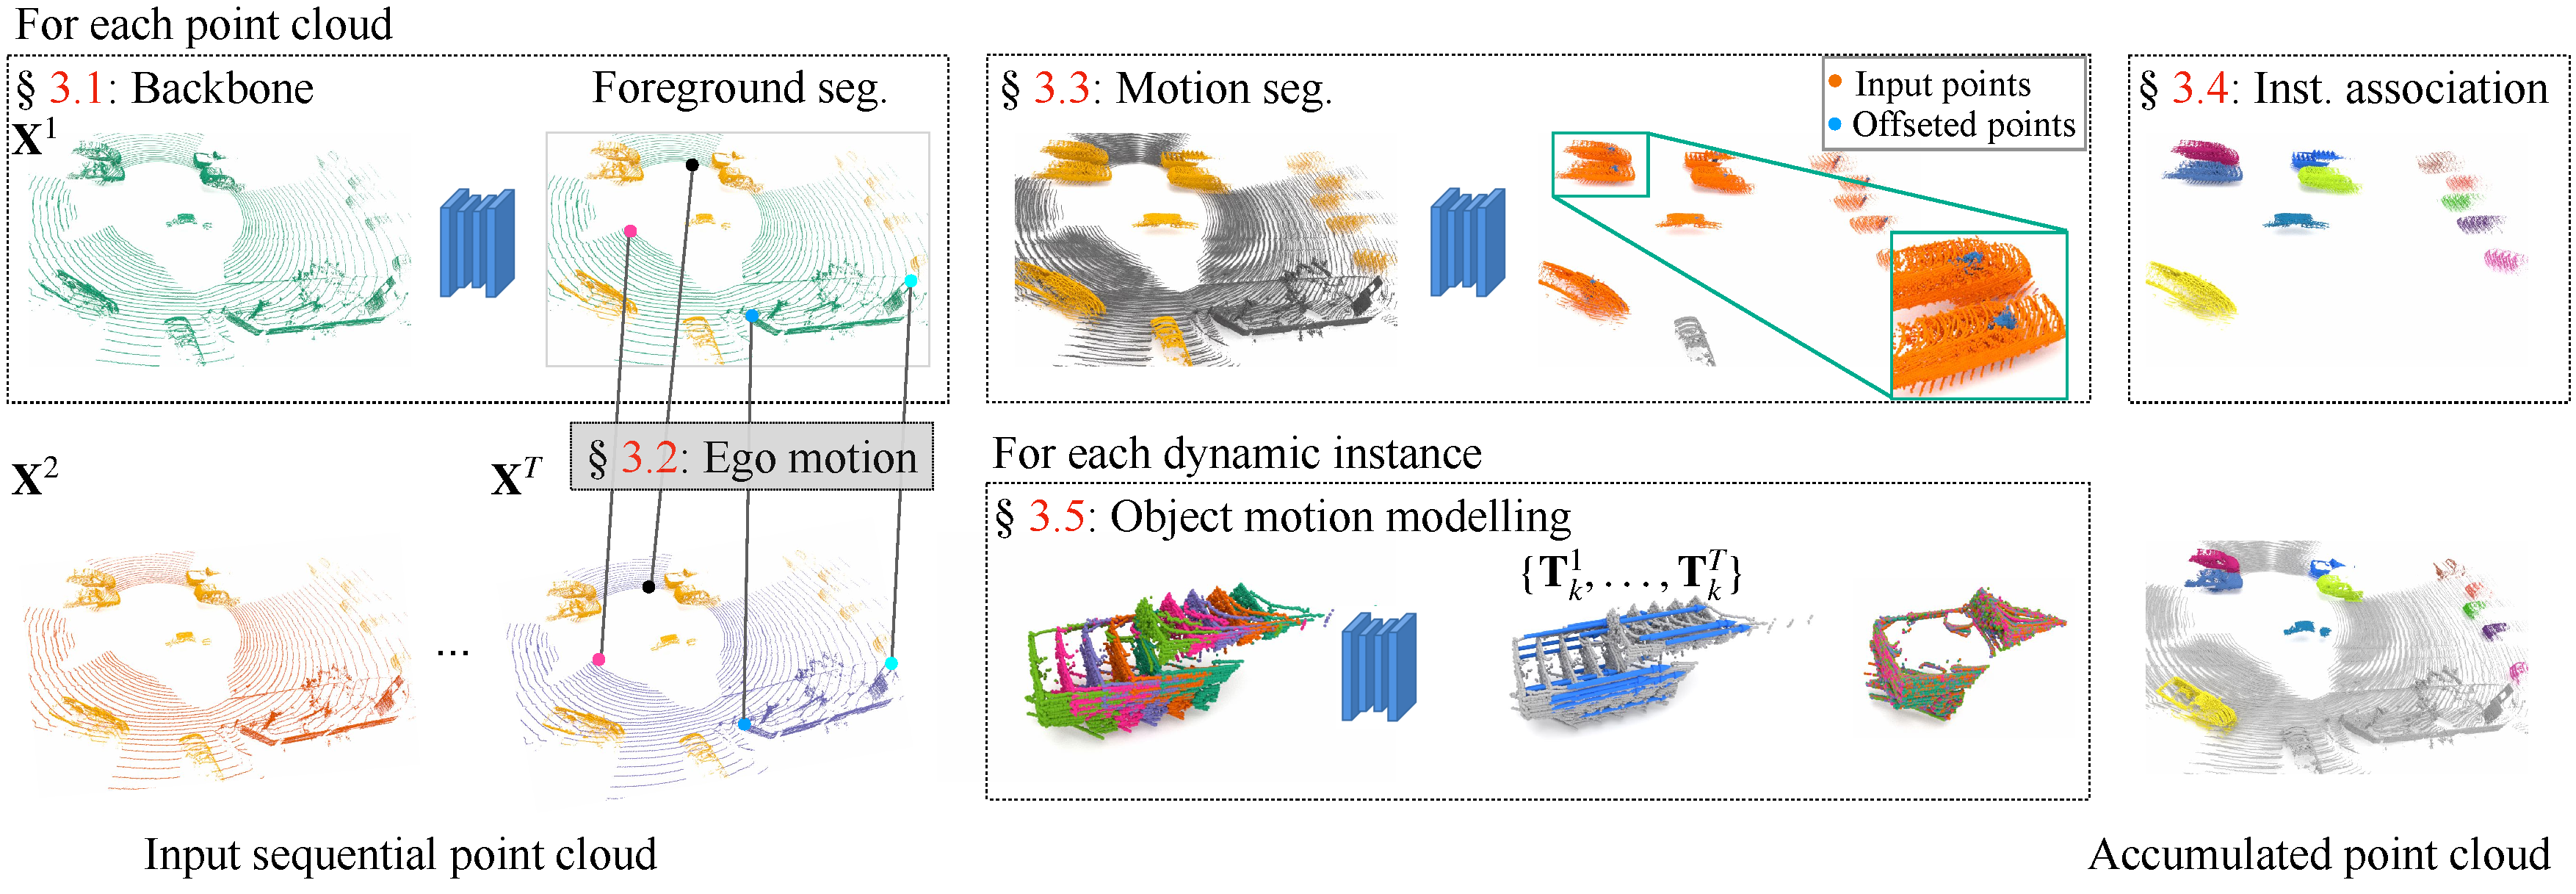
\includegraphics[width=1.0\textwidth]{Figures/overview.pdf}
        \caption{
        Overview of \dynfl. Our method takes LiDAR scans and tracked bounding boxes of dynamic vehicles as input. \dynfl first decomposes the scene into a static background and $N$ dynamic vehicles, each modelled using a dedicated neural field. These neural fields are then composed to re-simulate LiDAR scans in dynamic scenes. Our composition technique supports various scene edits, including altering object trajectories, removing and adding reconstructed neural assets between scenes.
    }
    \label{fig:main}
\end{figure*}

We introduce a neural representation for the purpose of reconstructing and manipulating LiDAR scans of dynamic driving scenes. 
Counterfactual re-simulation is an emerging application in the realm of autonomous driving, offering a unique approach to examining "what if" scenarios. This method involves creating a reconstruction of a real-world event, termed as \textit{digital twin} and then applying various modifications to it. These could include altering the environmental conditions, changing the action of some agent, or introducing additional scene elements. Analyzing the outcomes of these edited scenarios provides insights into the functioning of the perception system, moreover they can be used to obtain training data for rare situations.

The essence of counterfactual re-simulation is the capability to authentically recreate variations of the original, factual observation. We address this challenge in the context of LiDAR on autonomous vehicles (AV). Existing approaches to LiDAR re-simulation have important limitations. Conventional simulators such as CARLA~\cite{dosovitskiy2017carla} and NVIDIA DRIVE Sim are capable of modeling LiDAR sensors. However, their reliance on manually designed 3D simulation assets requires significant human effort. LiDARsim~\cite{manivasagam2020lidarsim} aims to remedy this by reconstructing vehicles and scenes from real measurements. While producing encouraging results, its two-stage LiDAR modeling lacks realism, particularly in terms of physical effects like multi-returns and reflected intensity, which were shown 
 to matter for downstream processing~\cite{guillard2022learning}. Following NeRF's~\cite{mildenhall2020nerf} success in camera view synthesis, some works have applied neural fields for LiDAR modeling~\cite{Huang2023nfl, tao2023lidar, zhang2023nerf}. In particular, Neural LiDAR Fields (NFL)\cite{Huang2023nfl} developed a physically inspired LiDAR volumetric rendering scheme that accounts for two-way transmittance and beam width, allowing faithful recovery of secondary returns, intensity, and ray drops. These models are, however, limited to static scenes that do not change while multiple input views are scanned, and are thus of limited use for re-simulation in the presence of moving traffic. Recently, UniSim~\cite{yang2023unisim} followed Neural Scene Graph~\cite{Ost_2021_CVPR} in modeling road scenes as sets of movable NeRF instances on top of a static background. UniSim introduced a unified synthesis approach for camera and LiDAR sensors, but ignored physical sensor properties like two-way transmittance and beam width~\cite{Huang2023nfl}.

We present \dynfl, a novel approach for re-simulating LiDAR views of driving scenarios. Our method builds upon a neural SDF that enables an accurate representation of scene geometry, while at the same time enforcing physical accuracy by modeling two-way transmittance, like NFL~\cite{Huang2023nfl}. 
% Our method builds upon UniSim's SDF representation and scene decomposition, but enhances the physical accuracy by incorporating two-way transmittance modeling, as introduced in NFL.
%
Our primary contribution is a method for compositing neural fields that accurately integrates LiDAR measurements from individual fields representing different scene assets. With the help of a ray drop test, we effectively manage occlusions and transparent surfaces. This not only ensures physical accuracy, but also facilitates the inclusion of assets reconstructed from a variety of static and dynamic scenes, thereby enhancing control over the simulated content. Our method bridges the gap between the physical fidelity of the re-simulation and flexible editing of dynamic scenes.
%
We validate \dynfl with both synthetic and real-world data, focusing on three key areas: \textit{(i)} high-quality view synthesis, \textit{(ii)} perceptual fidelity, and \textit{(iii)} asset manipulation. We find that our approach outperforms baseline models \wrt both range and intensity. Its synthetic outputs also show higher agreement with real scans in terms of object detection and segmentation. Furthermore, \dynfl enables not only removal, duplication and repositioning of assets within the same scene, but also the inclusion of assets reconstructed in other scenes, paving the way for new applications.


% In the rapidly evolving field of computer vision, novel view synthesis has become a groundbreaking technique, especially in the realm of image-based rendering. Pioneered by technologies like NeRF~\cite{mildenhall2020nerf}, it allows for the creation of photo-realistic views from a given set of data. However, the application of these principles to LiDAR data, which inherently deals with point clouds, introduces a complex set of challenges and opportunities that are distinct from traditional image-based approaches.

% Historically, methods like LiDARsim~\cite{manivasagam2020lidarsim} have paved the way for such advancements, yet they exhibit limitations. Specifically, LiDARsim operates by first extracting an explicit scene representation and then performing ray-surfel casting to synthesize LiDAR scans. This approach, while innovative, is susceptible to inaccuracies due to point cloud noise and typically results in lower reconstruction quality. This limitation leads to a significant domain gap when compared to ground truth LiDAR scans. Our previous work, Neural Lidar Fields (NFL)~\cite{Huang2023nfl}, marked a substantial improvement in modeling LiDAR scenes with neural fields and incorporating the physical characteristics of LiDAR beams. Despite its state-of-the-art performance in geometry reconstruction, NFL was limited to static scenes and did not address the complexities of dynamic environments.

% In dynamic scenarios, particularly in automotive or robotics contexts, capturing the constant motion of elements like vehicles and pedestrians is crucial. Our work seeks to bridge this gap by extending the principles of NFL to dynamic settings. Prior approaches that tackle the dynamic scenes, such as LiDARsim~\cite{manivasagam2020lidarsim}, have adopted a reconstruct-then-simulate process, resulting in inferior geometric fidelity. Meanwhile, other neural-fields-based explorations like Neural Scene Graph~\cite{Ost_2021_CVPR} and UniSim~\cite{yang2023unisim} focus on image-based rendering or sensor fusion, neglecting LiDAR-specific attributes.

% In this context, our work contributes in several ways:
% \textbf{1.)} Improved Geometry Quality: We adopt a Signed Distance Function (SDF)-based volume rendering approach, specifically tailored to the active sensor characteristics of LiDAR beam. This method acknowledges and leverages the intricacies of how LiDAR sensors capture data, resulting in reconstructions of higher fidelity and geometric accuracy.
% \textbf{2.)} Innovative Neural Fields Composition: Our methodology introduces a novel technique for the composition of multiple neural fields. This approach significantly enhances the rendering process, allowing for seamless integration and higher-quality synthesis of dynamic views.

% Our paper delves into the technicalities of Dynamic Neural LiDAR Fields, elaborating on the methods and innovations that enable the synthesis of dynamic views from LiDAR data. We present extensive experimental results that showcase the effectiveness of our approach in dynamic environments, illustrating how our contributions extend the applicability of neural LiDAR fields. Through this work, we provide a valuable resource for researchers in computer vision, contributing to the broader discourse on LiDAR novel view synthesis for dynamic scenes.


\section{Related work}
\paragraph{Neural radiance fields and volume rendering}
Neural Radiance Fields (NeRF)~\cite{mildenhall2020nerf} have demonstrated remarkable success in novel-view image synthesis through neural volume rendering. These fields are characterized by the weights of Multilayer Perceptrons (MLPs), which enable the retrieval of volume density and RGB colors at any specified point within the field for image compositing via volume rendering. Several studies~\cite{barron2021mip,barron2022mip,verbin2022ref,chen2022tensorf,fridovich2022plenoxels} have subsequently advanced NeRF's rendering quality by addressing challenges such as reducing aliasing artifacts~\cite{barron2021mip}, scaling to unbound large-scale scenarios~\cite{barron2022mip}, and capturing specular reflections on glossy surfaces~\cite{verbin2022ref}.
Certain works~\cite{chen2022tensorf,fridovich2022plenoxels,mueller2022instant,kerbl20233d} have explored more effective representations of radiance fields. TensorsRF~\cite{chen2022tensorf} employs multiple compact low-rank tensor components, such as vectors and matrices, to represent the radiance field. Plenoxels~\cite{fridovich2022plenoxels} accelerates NeRF training by replacing MLPs with explicit plenoptic elements stored in sparse voxels and factorizing appearance through spherical-harmonic functions.
M\"uller et al.~\cite{mueller2022instant} achieved a substantial acceleration in rendering speed by employing a representation that combines trainable multi-resolution hash encodings (MHE) with shared shallow MLP networks. Kerbel et al.~\cite{kerbl20233d} introduce a novel volume rendering method utilizing 3D Gaussians to represent the radiance field and rendering images based on visibility-aware splatting of 3D Gaussians.


\paragraph{Dynamic neural radiance fields} 
Neural fields \cite{xie2022neural} can be extended to represent dynamic scenes. On top of the \textit{canonical} scene representation, some methods~\cite{pumarola2020d, park2021nerfies, park2021hypernerf,yuan2021star} additionally model the 4D deformation fields. Meanwhile, some other works learn a space-time correlated~\cite{kplanes_2023, li2020neural, attal2023hyperreel, liu2023robust}, or decomposed~\cite{turki2023suds,wu2022d,yang2023emernerf} neural field to encode the 4D scenes, achieving fine-grained reconstruction of the geometry and the appearance.
%
Some other methods decompose the scene into static and dynamic parts, and model each dynamic actor with dedicated neural fields. 
Neural Scene Graph~\cite{Ost_2021_CVPR} and Panoptic Neural Fields~\cite{KunduCVPR2022PNF} treat every dynamic object in the scene as a node, and synthesize photo-realistic RGB images by jointly rendering from both dynamic nodes and static background. UniSim\cite{yang2023unisim} employs neural SDF representation to model dynamic scenes in driving scenarios, and render in a similar way to Neural Scene Graph~\cite{Ost_2021_CVPR}.


\paragraph{Neural surface representation}
A fundamental challenge for NeRF and its variants involves accurately recovering the underlying 3D surface from the implicit radiance field. Surfaces obtained by thresholding on the volume density of NeRF often exhibit noise~\cite{wang2021neus, yariv2021volume}. To address this, implicit surface representations like Occupancy~\cite{niemeyer2020differentiable, oechsle2021unisurf} and signed distance functions (SDF)~\cite{wang2021neus, yariv2021volume, yu2022monosdf, sun2022neural, wang2022hf, zuo2023incremental, li2023neuralangelo, wang2023neus2} in grid maps are commonly integrated into neural volume rendering techniques.

NeuS~\cite{wang2021neus} introduces a neural SDF representation for surface reconstruction, proposing an unbiased weight function for the appearance composition process in volume rendering. Similarly, VolSDF~\cite{yariv2021volume} models scenes with a neural SDF and incorporates the SDF into the volume rendering process, advocating a sampling strategy of the viewing ray to bound opacity approximation error. Neuralangelo~\cite{li2023neuralangelo} improves surface reconstruction using the multi-resolution hash encoding (MHE)~\cite{mueller2022instant} and SDF-based volume rendering~\cite{wang2021neus}. While these methods might deliver satisfying dense surface reconstructions, their training is time-consuming, taking hours for a single scene.
Voxurf~\cite{wu2022voxurf} offers a faster surface reconstruction method through a two-stage training procedure, recovering the coarse shape first and refining details later. Wang et al.~\cite{wang2023neus2} expedites NeuS training to several minutes by predicting SDFs through a pipeline composed of MHE and shallow MLPs.

Many works also incorporate distances measured by LiDAR as auxiliary information to constrain the radiance field. For instance, works~\cite{chang2023neural, wang2023neural} render depth by accumulating volume density and minimizing depth discrepancies between LiDAR and render depth during training. Rematas et al.~\cite{rematas2022urban} enforces empty space between the actual surface and the ray origin.


\paragraph{LiDAR simulation} 
While simulators like CARLA~\cite{dosovitskiy2017carla} and AirSim~\cite{shah2018airsim} can simulate LiDAR data, they suffer from expensive human annotation requirements and a notable sim-to-real gap due to limited rendering quality. Generative model-based methods for LiDAR synthesis~\cite{caccia2019deep,zyrianov2022learning} offer an alternative but often lack control and produce distorted geometries~\cite{li2023pcgen}.
Learning-based approaches~\cite{li2023pcgen,fang2020augmented,manivasagam2020lidarsim} try to enhance realism by transferring real scan properties to simulations. For example, \cite{guillard2022learning} uses a RINet trained on RGB and real LiDAR data to augment simulated scan qualities. LiDARsim~\cite{manivasagam2020lidarsim} employs ray-surfel casting with explicit disk surfels for more accurate simulations.
Huang et al.~\cite{Huang2023nfl} proposed Neural LiDAR Fields (NFL), combining neural fields with a physical LiDAR model for high-quality synthesis, although it's limited to static scenes and can produce noisy outputs due to its unconstrained volume density representation.
UniSim~\cite{yang2023unisim} constructs neural scene representations from realistic LiDAR and camera data, using SDF-based volume rendering for sensor measurement generation at novel viewpoints.


\section{Dynamic Neural Scene Representation}

\paragraph{Problem statement} 
Consider a set of LiDAR scans $\mathcal{X} = \{\mathbf{X}_t\}_{t=1}^T$ that have been compensated for ego-motion, along with tracked bounding boxes\footnote{We assume that the ground truth object detection and tracking annotations are available.} for dynamic vehicles $\mathcal{B} = \{\mathbf{B}_t^v\}_{v=1}^{N}$, where $T$ represents the total number of LiDAR scans, and $N$ is the count of dynamic vehicles. Each scan $\mathbf{X}_t$ is composed of $n_t$ rays, each ray $\mathbf{r}$ is described by the tuple $(\origin, \dir, \zeta, \intensity, \pdrop)$, where $\origin$ and $\dir$ denote the ray's origin and direction, $\zeta$ and $\intensity$ represent range and intensity values, and $\pdrop \in \{0,1\}$ indicates whether the ray is dropped or not due to insufficient returned radiant power.


The goal is to reconstruct the scene with a static-dynamic decomposed neural representation, that can enable the rendering of LiDAR scan $\mathbf{X}_{\text{tgt}}$ from novel viewpoint $\mathbf{T}_{\text{tgt}}$. This setup also facilitates various object manipulations, including altering object trajectories, and inserting or removing objects from the scene. The overview of our method is given in~\cref{fig:main}.

\subsection{Neural Scene Decomposition} \label{sec: decomposition}
We leverage the inductive bias that driving scenes can be decomposed into a static component and $N$ rigidly-moving dynamic components~\cite{huang2022dynamic,gojcic2021weakly}. Consequently, we establish $N+1$ neural fields. The neural field $\mathbf{F}_{\text{static}}$ is designated for the static component of the scene, capturing the unchanging background elements. Concurrently, the set of neural fields $\{\mathbf{F}^v\}_{v=1}^{N}$ is used to model the $N$ dynamic entities, specifically the vehicles in motion.



\paragraph{Neural field for static background} 
The static background is encoded into a neural field $\mathbf{F}_\text{static}: (\x, \dir) \mapsto (s, \intensity, \pdrop)$ that estimates the signed distance $s$, intensity $\intensity$, and ray drop probability $\pdrop \in [0,1]$ given the point coordinates $\x$ and the ray direction $\dir$. In practice, we first use a multi-resolution hash encoding (MRH)~\cite{mueller2022instant} to map each point to its positional feature $\posfeat \in \real^{32}$, and project the view direction onto the first 16 coefficients of the spherical harmonics basis, resulting in $\dirfeat$. Subsequently, we utilize three Multilayer Perceptrons (MLPs) to estimate the scene properties as follows:
\begin{equation}
(s, \geofeat) = f_s(\posfeat), \quad \intensity = f_{\intensity}(\rayfeat), \quad \pdrop = f_{\text{drop}}(\rayfeat).
\end{equation}
Here, $f_s, f_e,$ and $f_{\text{drop}}$ are three MLPs, $\rayfeat \in \mathbb{R}^{31}$ represents the ray feature and is constructed by concatenating the per-point geometric feature and the directional feature. The geometric feature is denoted as $\geofeat \in \mathbb{R}^{16}$. For more implementation details, please refer to the appendix. 

\begin{figure}[t]
    \centering
        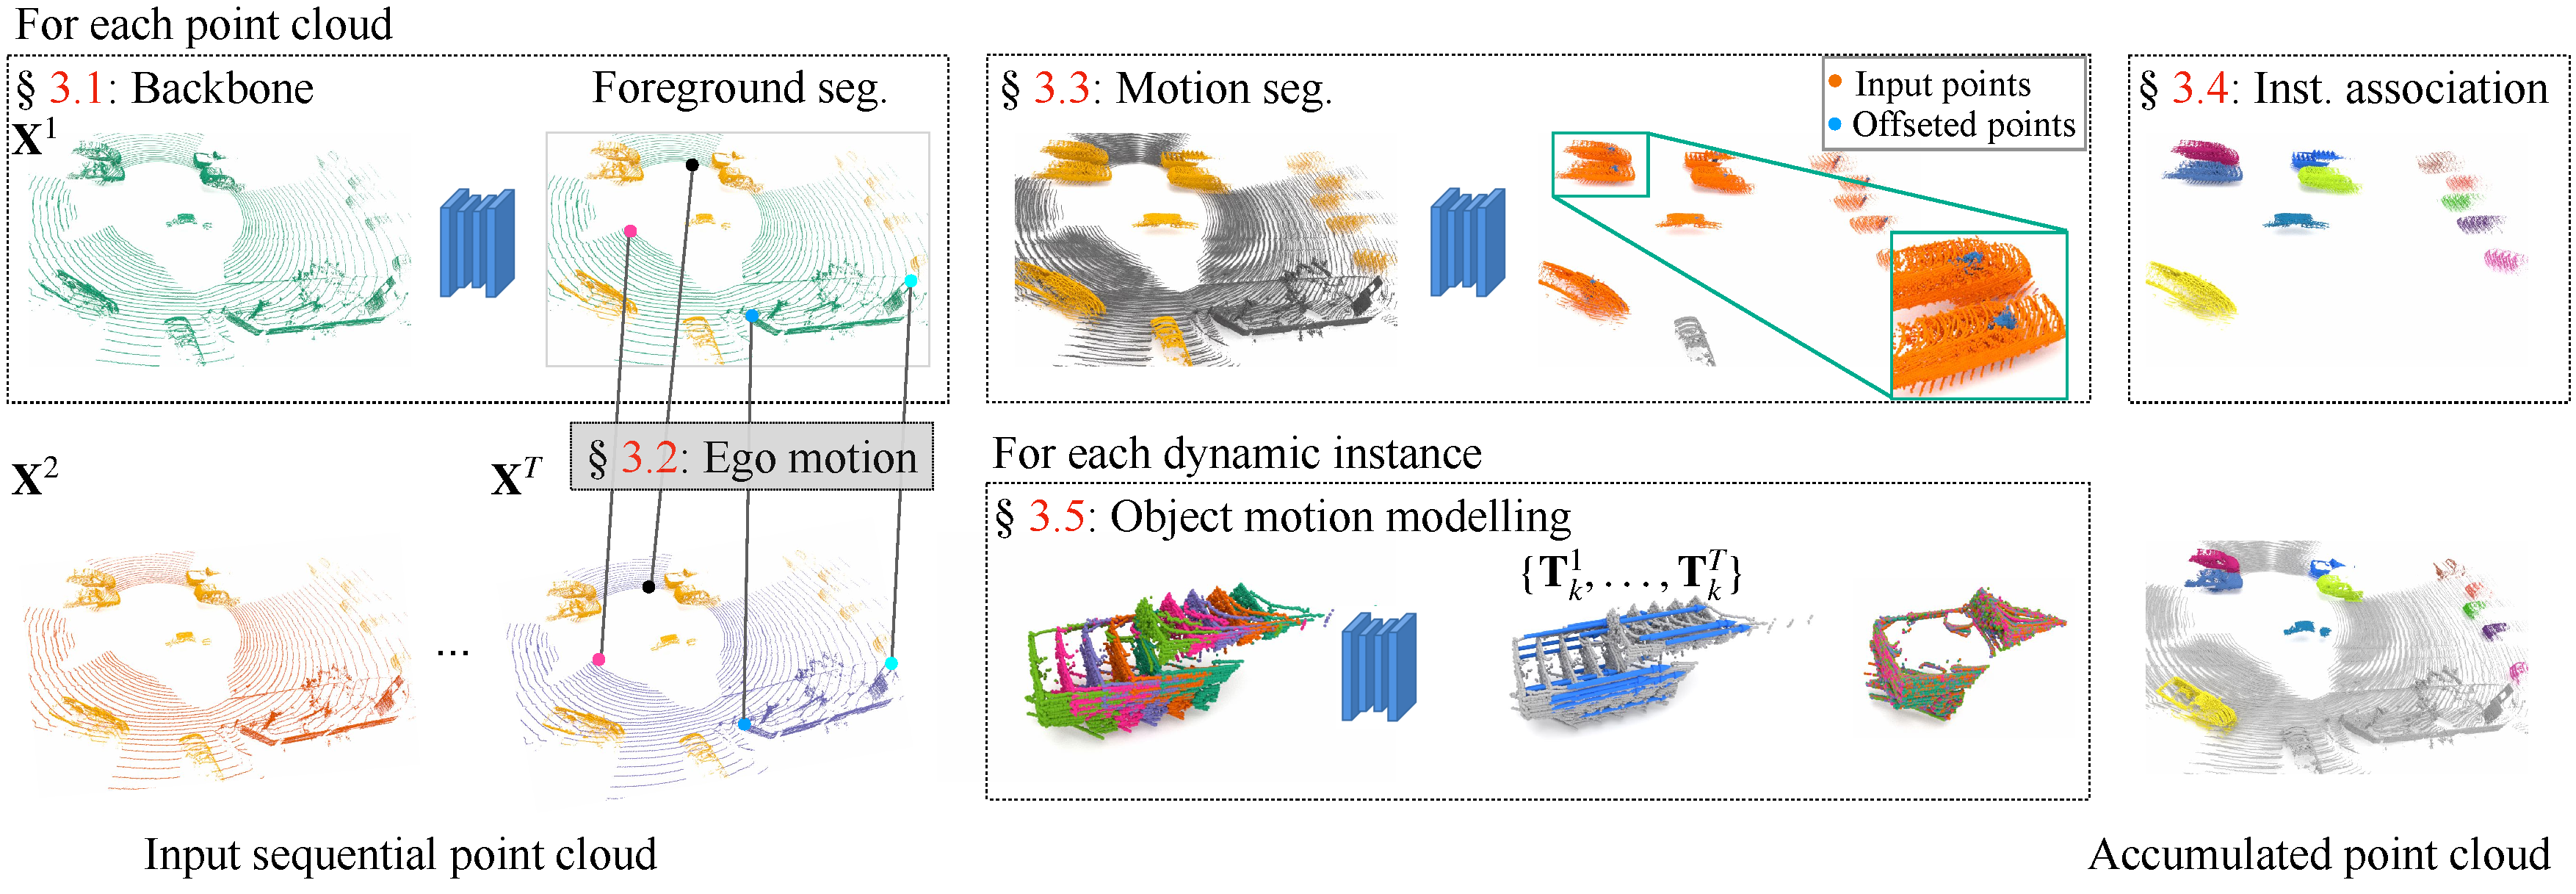
\includegraphics[width=1.0\columnwidth]{Figures/overview.pdf}
        \caption{
        Overview of \dynfl. Our method takes LiDAR scans and tracked bounding boxes of dynamic vehicles as input. \dynfl first decomposes the scene into a static background and $N$ dynamic vehicles, each modelled using a dedicated neural field. These neural fields are then composed to re-simulate LiDAR scans in dynamic scenes. Our composition technique supports various scene edits, including altering object trajectories, removing and adding reconstructed neural assets between scenes.
    }
    \label{fig:main}
\end{figure}


\paragraph{Neural fields for dynamic vehicles} 
LiDAR scans collected over time are often mis-aligned due to the motion of both the sensor and other objects in the scene. Despite applying ego-motion for aligning static background points, dynamic object points remain blurred along their trajectories. Our approach to constructing a dynamic neural scene representation is grounded in the assumption that each dynamic object only undergoes rigid motion. Therefore, we can first align them over time and reconstruct them in their \textit{canonical} coordinate frame, and then render them over time by reversing the alignment of the neural field.

Specifically, consider a dynamic vehicle $v$ 
occurring in LiDAR scans $\{\mathbf{X}^v_t\}_{t=1}^{T}$ along with the associated bounding boxes $\{\mathbf{B}^v_t \in \mathbb{R}^{3\times 8}\}_{t=1}^{T}$ in the world coordinate framework. Here each bounding box is defined by its eight corners, and the first bounding box $\mathbf{B}^v_1$ is considered as the \textit{canonical} box. We estimate the relative transformations $\{\mathbf{T}_t \in \text{SE}(3)\}_{t=2}^{T}$ between the remaining $T-1$ bounding boxes and the canonical box, expressed as $\mathbf{B}_1^v = \mathbf{T}_t \mathbf{B}_t^v$\footnote{$\mathbf{T}\mathbf{B} = \mathbf{R}\mathbf{B} + \mathbf{t}$, where $\mathbf{R}$ and $\mathbf{t}$ are the rotation and translation components of $\mathbf{T}$.}. 
Subsequently, all LiDAR measurements on the object are transformed and accumulated in its canonical coordinate frame. The vehicle $v$ is then reconstructed in its canonical space, akin to the static background, using a neural field $\mathbf{F}^v$. To render the dynamic vehicle at timestamp $t$, the corresponding rigid transformation is applied to the queried rays. The dynamic neural field can thus be expressed as: $\mathbf{F}^v_t: (\mathbf{T}_{t}\x, \mathbf{T}_{t}\dir) \mapsto (s, \intensity, \pdrop)$. The rendering process for $\mathbf{F}^v$ is the same as rendering for static neural field $\mathbf{F}_{\text{static}}$.



\section{Neural rendering of the dynamic scene}
In this section, we present the methodology for rendering LiDAR scans from the neural scene representation. We begin by revisiting the density-based volume rendering formulation for active sensors~\cite{Huang2023nfl} in \cref{sec:vol_render_background}. Subsequently, we explore the extension of this formulation to SDF-based neural scene representation in \cref{sec:sdf_vol_render}. Finally, we provide a detailed discussion on rendering LiDAR measurements from individual neural fields in~\cref{sec:dynamic_nfl_rendering} and the process of composing results from different neural fields in \cref{sec:neural_fields_composition}.



\subsection{Volume rendering for active sensor} 
\label{sec:vol_render_background}
LiDAR utilizes laser beam pulses to determine the distance to the nearest reflective surface by analyzing full waveform profile of the returned radiant power. The radiant power $P(\zeta)$ from range $\zeta$ is the result of a convolution between the pulse power $P_e(t)$ and the impulse response $H(\zeta)$, defined as~\cite{hahner2021fog,hahner2022lidar,Huang2023nfl}:
\begin{equation}
    P(\zeta) = \int_0^{2\zeta/c} P_e(t) H(\zeta - \frac{ct}{2}) \; dt\;.
\label{eq:lidar}
\end{equation}
The impulse response $H(\zeta)$ is a product of the target and sensor impulse responses: $H(\zeta) = H_T(\zeta)\cdot H_S(\zeta)$, and the individual components are expressed as:
\begin{equation}
    H_T(\zeta) = \frac{\reflectance}{\pi} \cos(\theta) \delta(\zeta - \bar{\zeta})\;, \quad  H_s(\zeta) = \transmittance^2_{\zeta} \frac{A_e}{\zeta^2}\;,
\label{eq:ht}
\end{equation}
where $\reflectance$ represents the surface reflectance, $\theta$ denotes incidence angle, $\bar{\zeta}$ is the ground truth distance to the nearest reflective surface, $\transmittance_{\zeta}$ and $A_e$ describe the transmittance at range $\zeta$ and sensor's effective area, respectively. Due to the non-differentiability introduced by the indicator function $\delta(\zeta - \bar{\zeta})$, ~\cref{eq:lidar} is non-differentiable and is thus not suitable for solving the inverse problem. NFL~\cite{Huang2023nfl} solves it by extending it into a probabilistic formulation given by:
\begin{equation}
P(\zeta) = C \cdot \frac{T^2_{\zeta} \cdot \density_\zeta  \reflectance_\zeta}{\zeta^2} \cos(\theta)\;.
\label{eq:radiance}
\end{equation}
Here, $C$ accounts for the constant values, and $\sigma_\zeta$ represents the density at range $\zeta$. The radiant can be reconstructed using the volume rendering formulation:
\begin{equation}
      P
      =\!\sum_{j=1}^N \int_{\zeta_j}^{\zeta_{j+1}}\!\!C \frac{\transmittance^2_{\zeta} \cdot \density_\zeta \reflectance_\zeta}{\zeta^2} \cos(\theta_j) \; d\zeta
      =\!\sum_{j=1}^N w_j \reflectance_{\zeta_j}',
\label{eq:radiant_inter}
\end{equation}
where the weights $w_j = 2 \opacity_{\zeta_j} \cdot\prod_{i=1}^{j-1}(1 - 2 \opacity_{\zeta_i}).$
Here $\alpha_{\zeta_j}$ is the discrete opacity at range $\zeta_j$. Please refer to~\cite{Huang2023nfl} for more details.


\subsection{SDF-based volume rendering for active sensor} 
\label{sec:sdf_vol_render}
A neural scene representation based on probabilistic density often results in surfaces with noticeable noise due to insufficient surface regularization~\cite{wang2021neus}. To address this, we opt for a signed distance-based scene representation and establish the volume rendering formulation within the framework of an active sensor. Building upon SDF-based volume rendering for passive sensors~\cite{wang2021neus}, we compute the opaque density $\tilde{\density}_{\zeta_i}$ as follows:
\begin{equation}
\tilde{\density}_{\zeta_i} = \max\left(\frac{-\frac{{\textrm{d}}\Phi_s}{{\textrm{d}} \zeta_i}(f(\zeta_i))}{\Phi_s(f(\zeta_i))},0\right),
\label{eq:sigmoid_density}
\end{equation}
where $\Phi_s(\cdot)$ represents the Sigmoid function, $f(\zeta)$ evaluates the signed distance to the surface at range $\zeta$ along the ray $\ray$. 

Next, we substitute the density $\density$ in \cref{eq:radiant_inter} with opaque density from \cref{eq:sigmoid_density} and re-evaluate the radiant power and weights as:
\begin{equation}
      P
      =\!\sum_{j=1}^N \transmittance^2_{\zeta_j} \tilde{\alpha}_{\zeta_j} \reflectance_{\zeta_j}',\quad \tilde{w}_j = 2 \tilde{\opacity}_{\zeta_j} \cdot\prod_{i=1}^{j-1}(1 - 2 \tilde{\opacity}_{\zeta_i})\;.
\end{equation}
In this context, $\tilde{\alpha}_{\zeta_j}$ is computed as:
\begin{equation}
    \tilde{\alpha}_{\zeta_j} = \max\left(\!\frac{{\Phi_s(f(\zeta_j))}^2 -{\Phi_s(f(\zeta_{j+1}))}^2}{{2\Phi_s(f(\zeta_j))}^2},0\right).
    \label{eq:new_weights}
\end{equation}
Please refer to the appendix for more details.


\subsection{Volume rendering for LiDAR measurements}
\label{sec:dynamic_nfl_rendering}
Consider rendering the LiDAR measurements from a single neural field, we employ the hierarchical sampling\cite{wang2021neus} technique to sample a total of $N_s= N_u + N_i$ points along each ray, where $N_u$ points are uniformly sampled, and $N_i$ points are probabilistically sampled based on the weights along the ray, facilitating denser sampling in proximity to the surface. Subsequently, we compute the weights for the $N_s$ points following~\cref{eq:new_weights}. The rendering of range, intensity, and ray drop for each ray can be expressed through volume rendering as follows: $y_\text{est} = \sum_{j=1}^{N_s} w_j y_j$, where $y \in \{\zeta, \intensity, \pdrop\}$.


\subsection{Neural rendering for multiple fields}\label{sec:neural_fields_composition}
Our full neural scene representation comprises $N+1$ neural fields as discussed in ~\cref{sec: decomposition}. Rendering from all these fields for each ray during inference is computationally intensive. To address this, we implement a two-stage method. In the first stage, we identify the $k+1$ neural fields, where $k \geq 0$ represents the number of dynamic fields, that are likely to intersect with a given ray. The second stage involves rendering LiDAR measurements from these selected fields individually and then integrating them into a unified set of measurements.


\paragraph{Ray intersection test}
As outlined in~\cref{sec: decomposition}, each dynamic neural field is reconstructed in its unique canonical space, defined by a corresponding canonical box. To determine neural fields intersecting with a ray at inference time, we begin by estimating the transformations $\{\mathbf{T}_t^v\}_{v=1}^N$, which convert coordinates from the world framework to each vehicle's canonical space at timestamp $t$. These transformations are determined by interpolating the training set transformations using spherical linear interpolation (SLERP)~\cite{10.1145/325334.325242}. Following this, we apply transformations to the queried ray and run intersection tests with the canonical boxes of the scenes. 


\paragraph{Neural rendering from multiple neural fields}
 After identifying the $k+1$ neural fields that potentially intersect with a ray, we perform volume rendering on each field separately, yielding $k+1$ distinct sets of LiDAR measurements. Next, we evaluate the ray drop probabilities across these fields. A ray is deemed \textit{dropped} if all neural fields indicate a drop probability $\pdrop > 0.5$. For rays not classified as dropped, we sort the estimated ranges in ascending order and select the nearest one as our final range prediction. Correspondingly, the intensity value is extracted from the same neural field associated with this closest range.

\section{Neural Scene Optimisation} \label{sec:optmisation}
Given the set of LiDAR scans and the associated tracked bounding boxes of the dynamic vehicles, we optimise our neural scene representation by minimising the loss:
\begin{equation}
    \mathcal{L} = w_{\zeta} \mathcal{L}_{\zeta} +  w_{s} \mathcal{L}_{s} + w_{\text{eik}} \mathcal{L}_{\text{eik}} + w_{\intensity} \mathcal{L}_{\intensity} + w_{\text{drop}} \mathcal{L}_{\text{drop}},
    \label{loss}
\end{equation}
where $w_{*}$ denotes respective weights, and each individual loss term $\mathcal{L}_*$ is explained below.


\paragraph{Range reconstruction loss}
For range estimation, we employ L1 loss, defined as: $\mathcal{L}_{\zeta} = \frac{1}{|\mathcal{R}|}\sum_{\ray \in \mathcal{R}}|\zeta_{est} -\zeta_{gt}|$, where $\mathcal{R}$ denotes the set of LiDAR rays, $\zeta_{est}$ and $\zeta_{gt}$ correspond to the estimated and actual ranges, respectively. 


\paragraph{Surface points' SDF regularisation} \label{sec:surfacesdf}
Acknowledging that LiDAR points mostly come from actual surface, we introduce an additional SDF regularisation term $\mathcal{L}_{s}$ that penalizes surface points' SDF values: $\mathcal{L}_{s} = \frac{1}{|\mathcal{P}|}\sum_{\mathbf{p} \in \mathcal{P}}|s(\mathbf{p})|$. Here $\mathcal{P}$ denotes the set of surface points and $s({\mathbf{p}})$ represents the SDF value of the point $\mathbf{p}$.


\paragraph{Eikonal constraint}
Following~\cite{icml2020_2086}, we utilize the Eikonal loss, $\leik$, to regularize the SDF level set. This ensures the gradient norm of the SDF is approximately one at any queried point. The loss is computed as: $\leik = \frac{1}{|\mathcal{Z}|} \sum_{\mathbf{p} \in \mathcal{Z}}( \| \nabla s(\mathbf{p}) \|_2 - 1)^2$, where $\mathcal{Z}$ is the set of all the sampled points. To stablise the training procedure, we adopt a numerical approach~\cite{li2023neuralangelo} to compute $\nabla s(\pos)$ as: 
\begin{equation}
    \nabla s(\pos) = \frac{s \left( \pos + \boldsymbol{\epsilon} \right) - s \left(\pos - \boldsymbol{\epsilon} \right)}{2 \epsilon} \;,
    \label{eqn:central_diff_normal}
\end{equation}
where the numerical step size $\epsilon$ is set to be $10^{-3}$ meters.


\paragraph{Intensity Loss}
For intensity reconstruction, we apply L2 loss, defined as: $\mathcal{L}_{\intensity} = \frac{1}{|\mathcal{R}|}\sum_{\ray \in \mathcal{R}}(\intensity_{est} -\intensity_{gt})^2.$


\paragraph{Ray drop loss}
We follow~\cite{Huang2023nfl} to supervise the ray drop estimation with a combination of a binary cross entropy loss $\mathcal{L}_{bce}$ and a Lovasz loss $\mathcal{L}_{ls}$ \cite{berman2018lovasz} as:
\begin{equation}
     \mathcal{L}_{\text{drop}} = \frac{1}{|\mathcal{R}|} \sum_{\ray \in \mathcal{R}} \left(\mathcal{L}_{bce}(p_{d, est}, {p_{d, gt}}) + \mathcal{L}_{ls}(p_{d, est}, {p_{d, gt}}) \right)\;.
     \label{eq:raydrop_loss}
\end{equation}
It's worth noting that in the context of dynamic neural fields, during training, we incorporate all LiDAR rays that intersect with the objects' bounding boxes of the scenes. A ray is classified as \textit{dropped} either if it is labeled as such in the dataset or if it does not intersect with the actual surfaces of the dynamic vehicles (\eg rays that are close but in parallel to the surfaces). This approach enhances the accuracy and realism of the reconstructed dynamic neural fields, improving the rendering fidelity at inference time. 

\section{Experiments}
\begin{figure*}[t]
  \centering
   \includegraphics[width=1\textwidth]{Figures/errormap_dynamic_3.pdf}
   
   \caption{Qualitative comparison of range estimation on \textit{Waymo Dynamic} dataset. Dynamic vehicles are zoomed in, and points are color-coded by range errors~(-100 \bwrDyNFL~100 cm).
   }
   \label{fig:errormap_dynamic}
   
\end{figure*}








\subsection{Datasets and Evaluation Protocol}\label{sec:datasets}

\paragraph{Real-world dynamic scenes} 
We construct \textit{Waymo Dynamic} dataset by selecting four representative scenes from Waymo Open dataset~\cite{sun2020scalability}, with multiple moving vehicles inside. These scenes are comprised of sequences of 50 consecutive frames. For evaluation purposes, every fifth frame is designated for testing, while the other 40 frames are allocated for training.


\paragraph{Real-world static scenes}
We also evaluate our method on four static scenes as introduced in~\cite{Huang2023nfl}. There are two settings, \textit{Waymo Interp} applies the same evaluation protocol as \textit{Waymo Dynamic}, while \textit{Waymo NVS} employs a dedicated closed-loop evaluation to validate the real novel view synthesis performance. Please refer to NFL~\cite{Huang2023nfl} for more details about this setting. 
 


\paragraph{Synthetic static scenes}  
\textit{TownClean} and \textit{TownReal} are synthetic static scenes introduced in NFL~\cite{Huang2023nfl}. They consist of 50 LiDAR scans simulated in urban street environment, using non-diverging and diverging beams, respectively. 



\paragraph{Evaluation metrics}\label{sec:metrics}
To evaluate the LiDAR range accuracy, we employ a suite of four metrics: mean absolute errors~(MAE [cm]), median absolute errors~(MedAE [cm]), Chamfer distance~(CD[cm]) and MedAE for dynamic vehicles~(MedAE Dyn[cm]). For intensity evaluation, We report root mean square error~(RMSE).
%
In addition to our primary evaluations, we assess the re-simulated LiDAR scans' realism through two auxiliary tasks: object detection and semantic segmentation. For object detection, we calculate the \textit{detection agreement}~\cite{manivasagam2020lidarsim}, both for all vehicles (Agg.~[\%]) and specifically for dynamic vehicles (Dyn.$\;$Agg.~[\%]). Regarding semantic segmentation, we measure and report recall, precision, and the intersection over union (IoU[\%]). It's important to note that the predictions on the original LiDAR scans serve as our \textit{ground truth}, against which we compare the results obtained from the re-simulated scans.




\paragraph{Baseline methods}
Regarding LiDAR simulation on static scenes, NFL~\cite{Huang2023nfl} and LiDARsim\cite{manivasagam2020lidarsim} are two closest baselines to compare to. Additionally, we include i-NGP~\cite{mueller2022instant}, DS-NeRF~\cite{kangle2021dsnerf}, and URF~\cite{rematas2022urban} for comparison. As for simulation on dynamic scenes, we compare to LiDARsim~\cite{manivasagam2020lidarsim} and UniSim~\cite{yang2023unisim}\footnote{We re-implement LiDARsim~\cite{lee2015lidar} and UniSim~\cite{yang2023unisim} as they are not open-sourced.}. Please refer to the appendix for implementation details.


\begin{table}[t]
    \setlength{\tabcolsep}{4pt}
    \renewcommand{\arraystretch}{1.2}
	\centering
	\resizebox{\columnwidth}{!}{
    \begin{tabular}{l|ccccc}
    \toprule
    Method  & MAE $\downarrow$ &  MedAE $\downarrow$ & CD $\downarrow$ & MedAE Dyn $\downarrow$ & Intensity RMSE $\downarrow$\\
    \midrule
    LiDARsim~\cite{manivasagam2020lidarsim} & 170.1 & 11.5 & 31.1 &  16.0  & 0.10\\
    Unisim~\cite{yang2023unisim} & 35.6 & 6.1 & 14.3 &14.3 & \textbf{0.05}\\
    Ours~ & \textbf{30.8} & \textbf{3.0} & \textbf{10.9} &\textbf{8.5} & \textbf{0.05}\\
    \bottomrule
    \end{tabular}
    }
    
	\caption{Evaluation of LiDAR NVS on \textit{Waymo Dynamic} dataset.}
	\label{tab:waymodynamic}
\end{table}
\begin{table}[t]
    \setlength{\tabcolsep}{4pt}
    \renewcommand{\arraystretch}{1.2}
	\centering
	\resizebox{\columnwidth}{!}{
    \begin{tabular}{l|ccc|ccc|ccc|ccc}
    \toprule
    & \multicolumn{3}{c|}{TownClean}& \multicolumn{3}{c|}{TownReal} & \multicolumn{3}{c|}{Waymo interp.} & \multicolumn{3}{c}{Waymo NVS} \\
    Method  & MAE $\downarrow$ &  MedAE $\downarrow$ & CD $\downarrow$& MAE $\downarrow$ &  MedAE $\downarrow$ & CD $\downarrow$ & MAE $\downarrow$ &  MedAE $\downarrow$ & CD $\downarrow$ & MAE $\downarrow$ &  MedAE $\downarrow$ & CD $\downarrow$\\
    \midrule
    i-NGP~\cite{mueller2022instant} &42.2 &4.1 & 17.4 & 49.8 & 4.8 & 19.9 & \textbf{26.4} & 5.5 & \textbf{11.6} & \underline{30.4} & 7.3 & 15.3\\
    DS-NeRF~\cite{kangle2021dsnerf} &41.7 & 3.9 &16.6 & 48.9 & 4.4 & 18.8 & \underline{28.2} & 6.3 & 14.5 & 30.4 & 7.2 & 16.8 \\
    URF~\cite{rematas2022urban} &43.3&4.2&16.8& 52.1 & 5.1 & 20.7 & 28.2 & 5.4 & 12.9 & 43.1 & 10.0 & 21.2 \\
    LiDARsim~\cite{manivasagam2020lidarsim} &159.6&\underline{0.8}&23.5& 162.8 & 3.8 & 27.4 & 116.3 & 15.2 & 27.6 & 160.2 & 16.2 & 34.7 \\
    NFL\cite{Huang2023nfl}  &\underline{32.0}&2.3&\underline{9.0}& \underline{39.2} & \underline{3.0} & \underline{11.5} & 30.8 & \underline{5.1} & \underline{12.1}& 32.6 & \underline{5.5} & \underline{13.2}  \\
    Ours & \textbf{26.7} & \textbf{0.7} & \textbf{6.7} &\textbf{33.9}&\textbf{2.1}&\textbf{10.4}& 28.3 & \textbf{4.7} & 12.5 & \textbf{28.6} & \textbf{4.9} & \textbf{13.0} \\
    \bottomrule
    \end{tabular}
}
    
	\caption{Evaluation of LiDAR NVS on static scenes.}
	\label{tab:waymostatic}
\end{table}
\begin{figure}[t]
  \centering
   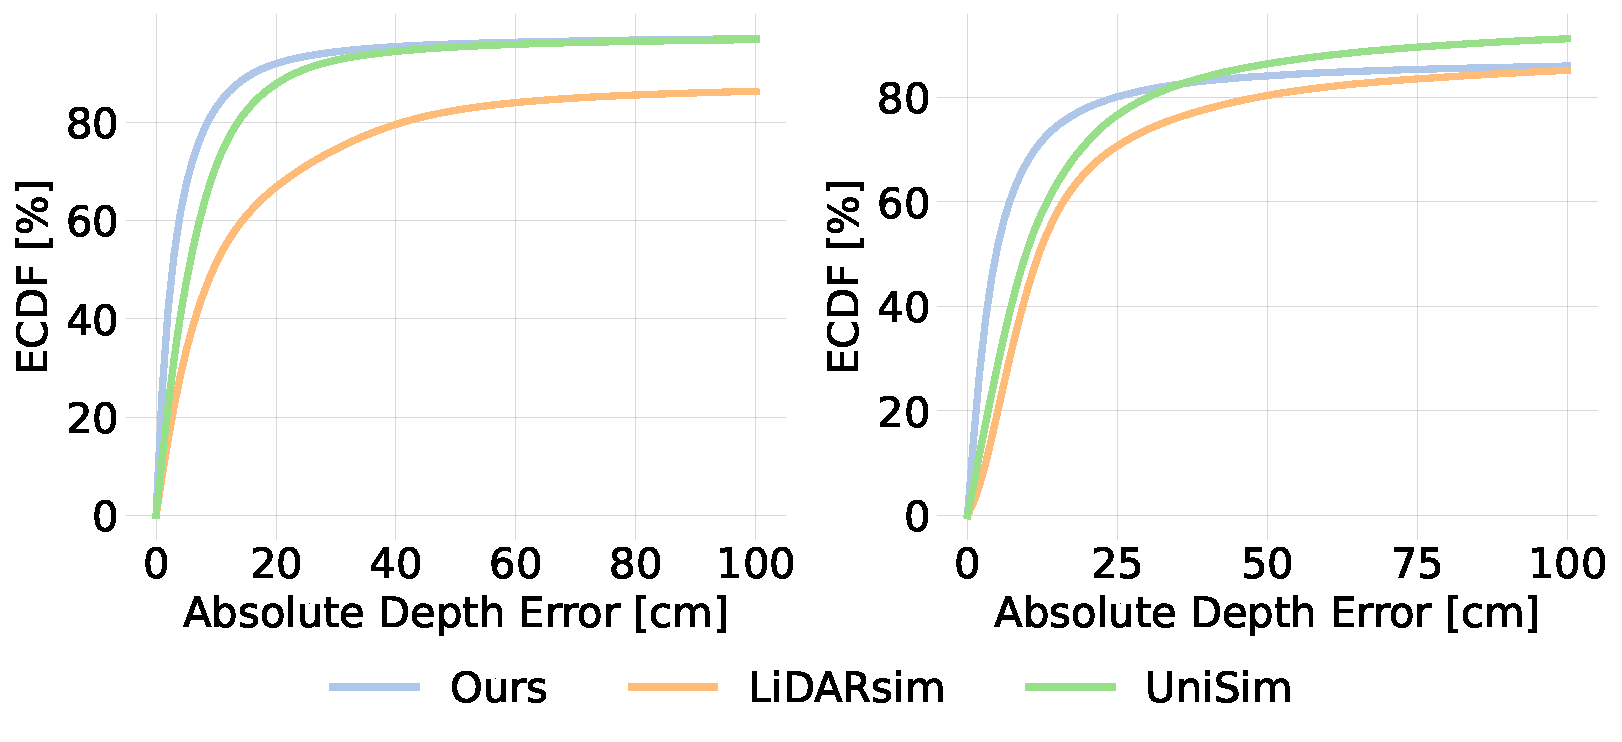
\includegraphics[width=1\columnwidth]{Figures/ecdf_3_methods.pdf}
   
        \caption{ECDF plots showcasing range errors across all the points (left) and specifically for points associated with dynamic vehicles (right). Our neural fields composition demonstrates superior performance over LiDARsim~\cite{manivasagam2020lidarsim} and UniSim~\cite{yang2023unisim}, especially in the context of dynamic vehicles.}
   \label{fig:ecdf}
   
\end{figure}
\begin{figure}[t]
    \centering
        \includegraphics[width=1\columnwidth]{Figures/errormap_static.pdf}
        
        \caption{Qualitative results of range estimation. Regions with gross errors (-100 \bwrDyNFL~100 cm) are highlighted.
        }
    \label{fig:error_map}
\end{figure}
\subsection{LiDAR Novel View Synthesis Evaluation} \label{sec:lidar_eval}
\paragraph{LiDAR NVS in dynamic scenes}
Quantitative comparisons with baseline methods are detailed in~\cref{tab:waymodynamic}. \dynfl notably outperforms LiDARsim~\cite{manivasagam2020lidarsim} and UniSim~\cite{yang2023unisim} in range reconstruction. This improvement is largely due to our SDF-based neural scene representation, which incorporates the physical aspects of LiDAR sensing. Additionally, our method employs a ray drop test when rendering multiple neural fields, leading to a more accurate reconstruction of dynamic vehicles, as evidenced in~\cref{fig:errormap_dynamic} and further supported by the data in~\cref{fig:ecdf}.


\begin{figure*}[t]
    \centering
        \includegraphics[width=1.0\textwidth]
        {Figures/sensor_manipulation.pdf}
        
        \caption{LiDAR novel view synthesis by changing sensor elevation angle~($\theta$), poses~($x,y,z$) and number of beams on \textit{Waymo Dynamic} dataset. The points are color-coded by the intensity values (0 \bwrDyNFL~0.25).}
    \label{fig:lidar_nvs}
\end{figure*}
\paragraph{LiDAR NVS in static scenes}
In addition to dynamic scenes, we evaluate \dynfl against baseline methods in static scenarios, with the results detailed in~\cref{tab:waymostatic} and~\cref{fig:error_map}. \dynfl excels in reconstructing geometry in most cases. A key observation is its superior performance in reconstructing planar regions (\eg the ground shown in~\cref{fig:error_map}), especially when compared to NFL~\cite{Huang2023nfl}, which also uses a neural field for surface representation. This improvement is largely due to the enhanced surface regularizations provided by our advanced SDF-based surface modeling approach.


\begin{table}[t]
    \setlength{\tabcolsep}{4pt}
    \renewcommand{\arraystretch}{1.2}
	\centering
	\resizebox{0.5\columnwidth}{!}{
    \small
    \begin{tabular}{l|ccc}
    \toprule
    Datasets  & MAE $\downarrow$ &  MedAE $\downarrow$ & CD $\downarrow$ \\
    \midrule
    TownClean~ & 26.7(\textcolor{green}{-1.5}) & 0.7(\textcolor{green}{-0.2}) & 6.7(\textcolor{green}{-0.5})\\
    Waymo Interp~ & 28.3 (\textcolor{red}{0.1}) & 4.7 (\textcolor{green}{-0.2}) & 12.5 (\textcolor{green}{-0.1})\\
    Waymo Dynamic~ & 30.8 (\textcolor{green}{-0.3}) & 3.0 (\textcolor{green}{-0.2}) & 10.9 (\textcolor{green}{-0.3})\\
    \bottomrule
    \end{tabular}
    }
    
	\caption{Ablation study of volume rendering for active sensing.}
	\label{tab:active_sensing}
\end{table}
\begin{table}[t]
    \setlength{\tabcolsep}{4pt}
    \renewcommand{\arraystretch}{1.2}
	\centering
	\resizebox{0.5\columnwidth}{!}{
    \small
    \begin{tabular}{l|ccc}
    \toprule
    Datasets  & MAE $\downarrow$ &  MedAE $\downarrow$ & CD $\downarrow$ \\
    \midrule
    TownReal~ & 33.9(\textcolor{green}{-3.3}) & 2.1(\textcolor{green}{-0.0}) & 10.4(\textcolor{green}{-1.2})\\
    Waymo Interp~ & 28.3 (\textcolor{green}{-0.3}) & 4.7 (\textcolor{green}{-0.1}) & 12.5 (\textcolor{green}{-0.3})\\
    \bottomrule
    \end{tabular}
    }
    
	\caption{Ablation study of the surface points' SDF regularisation.}
	\label{tab:surface_sdf}
\end{table}
\begin{figure}[t]
  \centering
   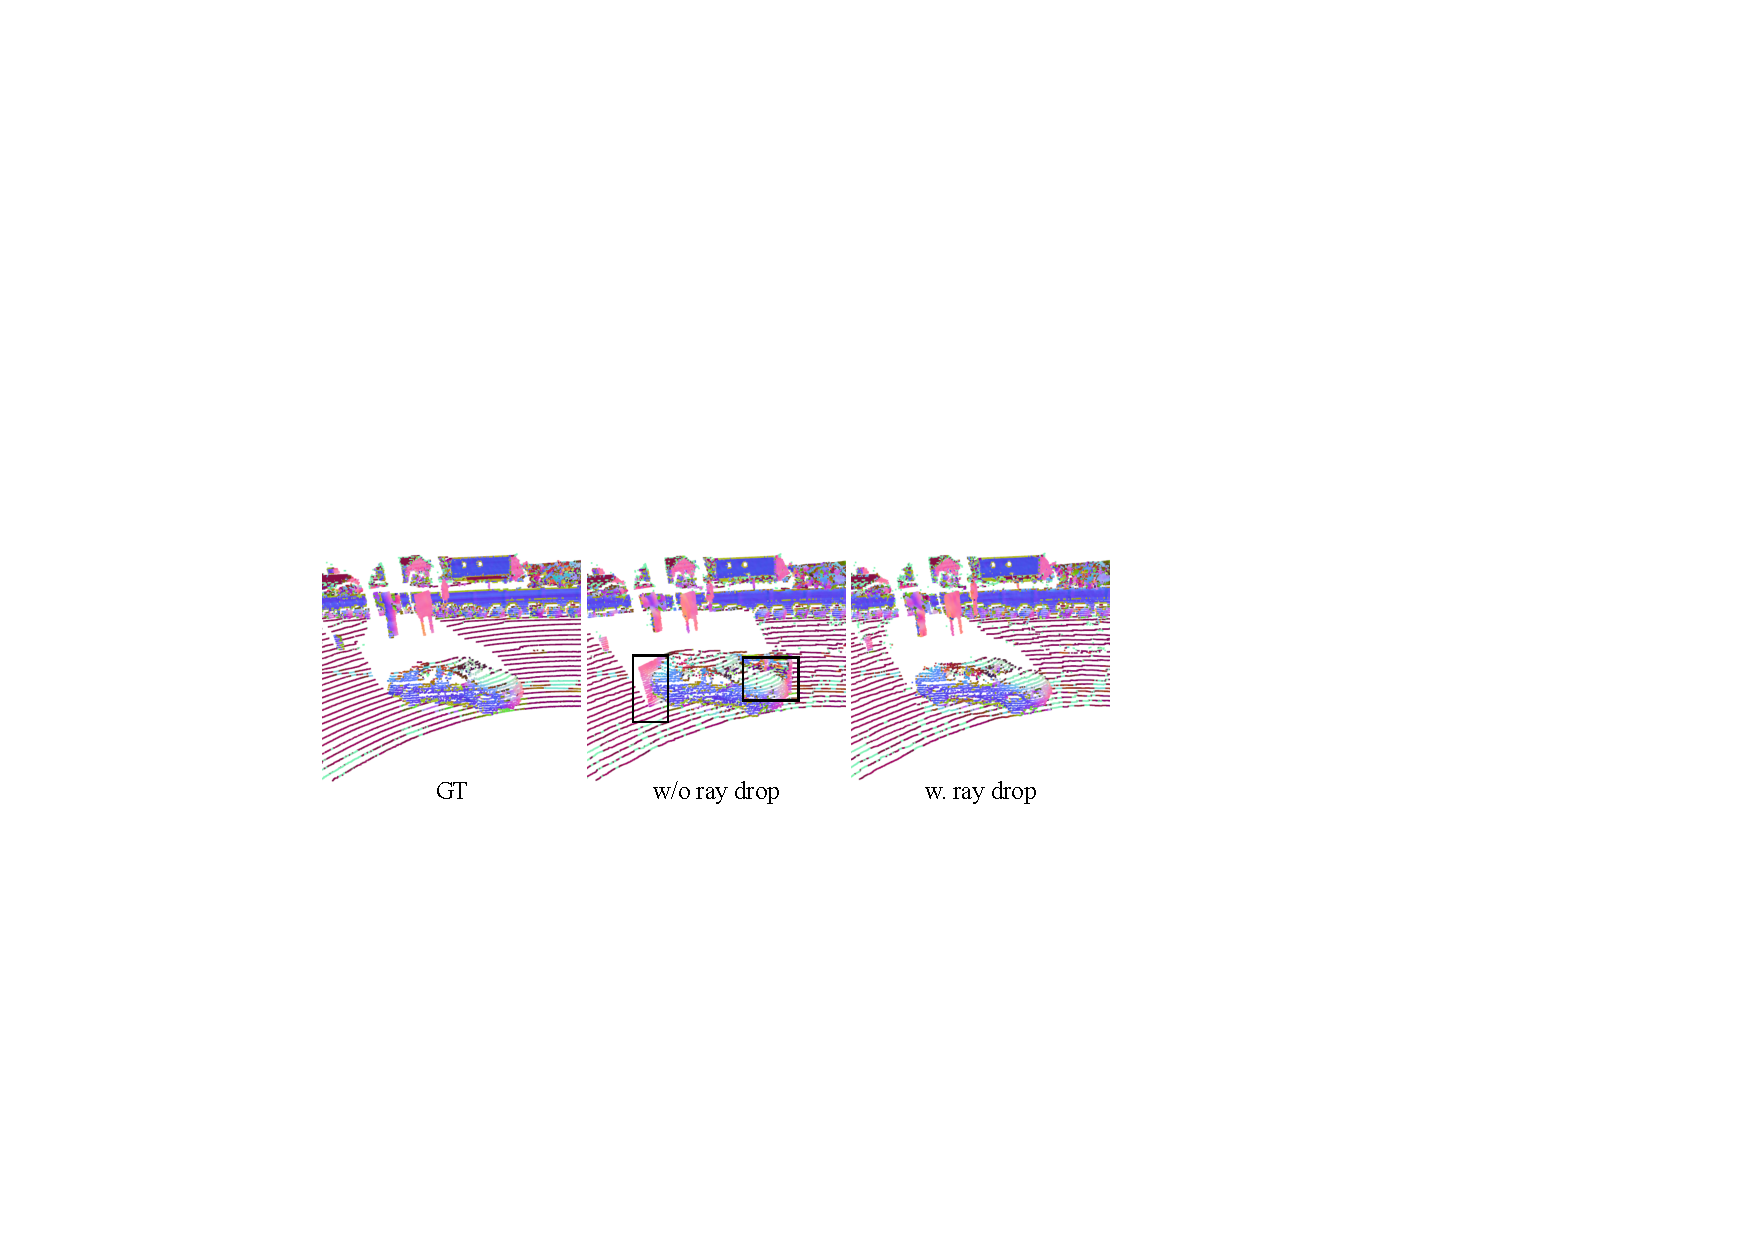
\includegraphics[width=1\linewidth]{Figures/intersectiontest.pdf}
   
   \caption{
   Qualitative results on \textit{Waymo Dynamic} dataset. Our model equipped with a ray drop module effectively composites multiple neural fields, re-simulating LiDAR scans of high quality.
   }
   % \caption{These figures exemplify the effectiveness of our field composition method leveraging ray drop probability from dynamic neural field. When all intersected rays are rendered for the dynamic neural field, noticeable artifacts appear due to disturbances from irrelevant fields (middle figure). The figures on the right showcase the complete composition method.
   % }
   % \caption{
   % }
    
   \label{fig:ablation_raydrop}
\end{figure}

\begin{figure}[t]
    \centering
        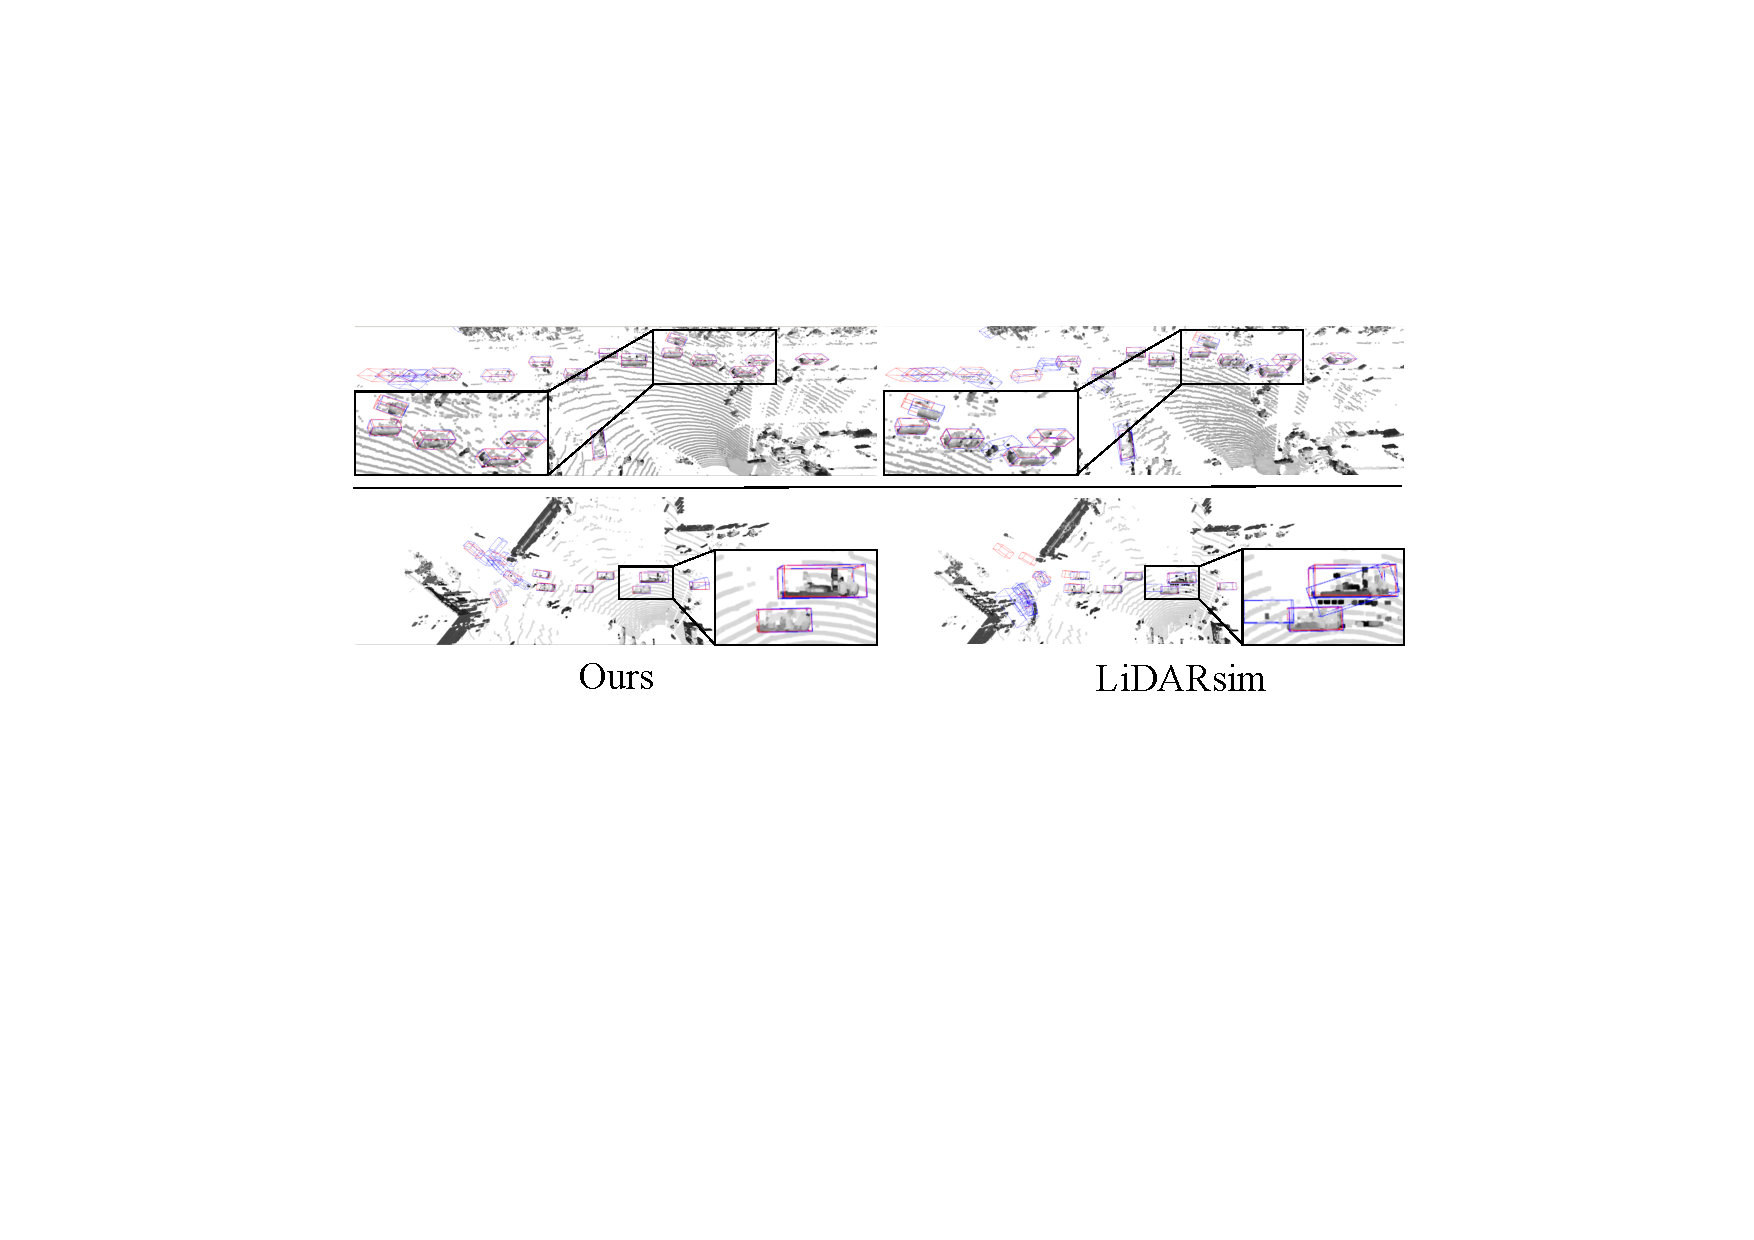
\includegraphics[width=0.8\columnwidth]{Figures/detection_result.pdf}
        \caption{Object detection results on \textit{Waymo Dynamic} dataset. The ground truth and predicted bounding boxes are marked in \textcolor{red}{red} and \textcolor{blue}{blue}, respectively.}
    \label{fig:detection}
    
\end{figure}
% \begin{table}[t]
% 	\centering
% 	\resizebox{0.8\columnwidth}{!}{
% 		\begin{tabular}{@{}lcccccccc@{}}
% 			\toprule
%              & \multicolumn{1}{c}{GT} & \multicolumn{3}{c}{Ours} & \multicolumn{3}{c}{LiDARSim\cite{manivasagam2020lidarsim}} \\
% 			  \cmidrule(r){2-2}\cmidrule(r){3-5} \cmidrule(l){6-8}
% 			Threshold & AP$\uparrow$ & \multicolumn{1}{c}{AP$\uparrow$}& \multicolumn{1}{c}{Agg.$\uparrow$}& \multicolumn{1}{c}{Dyn. Agg.$\uparrow$} & \multicolumn{1}{c}{AP$\uparrow$} & \multicolumn{1}{c}{Agg.$\uparrow$}& \multicolumn{1}{c}{Dyn. Agg.$\uparrow$} \\
% 			\midrule
% 			IoU$>$0.7 &0.85  &0.86 & \textbf{0.77}& \textbf{0.71}& \textbf{0.90} & 0.76 & 0.68\\
% 			IoU$>$0.5 &\textbf{0.98}  & 0.96 & \textbf{0.87}& \textbf{0.76}& 0.95 & 0.86& \textbf{0.76} \\
% 			\bottomrule
% 		\end{tabular}
% 	}
% 	\caption{Object detection results on \textit{Waymo Dyanmic} datasets.}
    
% 	\label{tab:detection}
% \end{table}

\begin{table}[t]
	\centering
		\begin{tabularx}{\columnwidth}{l|YYYYYYY}
			\toprule
             & \multicolumn{1}{c}{GT} & \multicolumn{3}{c}{Ours} & \multicolumn{3}{c}{LiDARSim\cite{manivasagam2020lidarsim}} \\
			  \cmidrule(r){2-2}\cmidrule(r){3-5} \cmidrule(l){6-8}
			Threshold & AP$\uparrow$ & \multicolumn{1}{c}{AP$\uparrow$}& \multicolumn{1}{c}{Agg.$\uparrow$}& \multicolumn{1}{c}{Dyn. Agg.$\uparrow$} & \multicolumn{1}{c}{AP$\uparrow$} & \multicolumn{1}{c}{Agg.$\uparrow$}& \multicolumn{1}{c}{Dyn. Agg.$\uparrow$} \\
			\midrule
			IoU$>$0.7 &0.85  &0.86 & \textbf{0.77}& \textbf{0.71}& \textbf{0.90} & 0.76 & 0.68\\
			IoU$>$0.5 &\textbf{0.98}  & 0.96 & \textbf{0.87}& \textbf{0.76}& 0.95 & 0.86& \textbf{0.76} \\
			\bottomrule
		\end{tabularx}
	\caption{Object detection results on \textit{Waymo Dyanmic} datasets.}
    
	\label{tab:detection}
\end{table}
% \begin{table}[t]
% \setlength{\tabcolsep}{4pt}
% \renewcommand{\arraystretch}{1.2}
% \centering
% \resizebox{0.8\columnwidth}{!}{
% \begin{tabular}{l|ccc|ccc}
% \toprule
% & \multicolumn{3}{c|}{Vehicle} & \multicolumn{3}{c}{Background} \\
% Method & Recall $\uparrow$ & Precision $\uparrow$ & IoU $\uparrow$ & Recall $\uparrow$ & Precision $\uparrow$ & IoU $\uparrow$ \\
% \midrule
% i-NGP~\cite{muller2022instant} & \underline{93.2} & 85.9 & 80.9 & 98.3 & \underline{99.2} & 97.6\\
% DS-NeRF~\cite{deng2021depth} & 90.7 & \underline{87.1} & 80.2 & \underline{98.5} & 98.9 & 97.4\\
% URF~\cite{rematas2021urban} & 87.8 & 81.7 & 73.7 & 98.0 & 98.4 & 96.5\\
% Lidarsim~\cite{manivasagam2020lidarsim} & 90.5 & 70.5 & 65.9 & 94.9 & 99.0 & 94.0\\
% NFL density~\cite{Huang2023nfl}& \textbf{95.9} & 87.0 & \textbf{83.9} & 98.3 & \textbf{99.5} & \textbf{97.8}\\
% Ours & 90.5 & \textbf{89.2} & \underline{82.3} & \textbf{98.8} & 98.9 & \underline{97.7}\\
% \bottomrule
% \end{tabular}
% }
% 
% \caption{Semantic segmentation results on \textit{Waymo NVS} dataset.}
% \label{tab:sem_seg_nvs}
% \end{table}



\begin{table}[t]
\setlength{\tabcolsep}{4pt}
\renewcommand{\arraystretch}{1.2}
\centering
\resizebox{0.99\columnwidth}{!}{
\begin{tabular}{l|ccc|ccc}
\toprule
& \multicolumn{3}{c|}{Vehicle} & \multicolumn{3}{c}{Background} \\
Method & Recall $\uparrow$ & Precision $\uparrow$ & IoU $\uparrow$ & Recall $\uparrow$ & Precision $\uparrow$ & IoU $\uparrow$ \\
\midrule
i-NGP~\cite{mueller2022instant} & 91.8 & 83.6 & 78.1 & 97.9 & 99.2 & 97.1\\
DS-NeRF~\cite{kangle2021dsnerf} & 89.3 & 84.8 & 77.3 & 98.1 & 98.8 & 97.0\\
URF~\cite{rematas2021urban} & 86.9 & 79.8 & 72.0 & 97.7 & 98.5 & 96.2\\
Lidarsim~\cite{manivasagam2020lidarsim} & 89.6 & 68.9 & 64.0 & 94.5 & 98.9 & 93.5\\
NFL~\cite{Huang2023nfl}& \textbf{94.5} & 84.8 & 80.9 & 97.8 & \textbf{99.4} & \textbf{97.3}\\
Ours & 90.5 & \textbf{88.4} & \textbf{81.1} & \textbf{98.5} & 98.7 & \textbf{97.3}\\
\bottomrule
\end{tabular}
}

\caption{Semantic segmentation results on \textit{Waymo NVS} dataset.}
\label{tab:sem_seg_nvs_ours}

\end{table}




\subsection{Ablation Study}
\paragraph{SDF-based volume rendering for active sensing}
We begin by assessing the efficacy of our SDF-based volume rendering for active sensor, the results are shown in~\cref{tab:active_sensing}. When compared to our baseline that uses the SDF-based volume rendering for passive sensing, \dynfl demonstrates enhanced performance in both synthetic (\textit{TownClean}) and real-world (\textit{Waymo Interp} and \textit{Waymo Dynamic}) datasets, indicating the importance of incorporating the physical sensing process of LiDAR in addressing the inverse problem.


\paragraph{Neural fields composition} 
To validate the efficacy of our two-stage neural field composition approach, we compare it with an alternative approach utilized in UniSim~\cite{yang2023unisim}. The results are shown in~\cref{tab:waymodynamic}. UniSim~\cite{yang2023unisim} blends different neural fields by sampling points from all intersected neural fields, followed by a single evaluation of volume rendering to produce the final LiDAR scan. In contrast, our method independently renders from each intersecting neural field first, and then combines these measurements into a final measurement using a ray drop test (\cf~\cref{fig:ablation_raydrop}). This approach leads to a notable improvement in geometry reconstruction over UniSim~\cite{yang2023unisim}, exemplified by our method halving the Median Absolute Error (MedAE) across all points. This enhancement is even more evident when focusing solely on points related to dynamic vehicles (\cf~\cref{fig:ecdf}).
% 

\paragraph{Surface points' SDF constraint}
We examine the importance of the surface points' SDF constraint discussed in ~\cref{sec:optmisation} on \textit{Town Real} and \textit{Waymo Interp} datasets. The results shown in \cref{tab:surface_sdf} suggest that our method yields improved geometry reconstruction quality by additionally enforcing LiDAR points to have zero SDF values. 


\subsection{Auxiliary Task Evaluations} 
\label{sec:downstream}
To assess the fidelity of our neural re-simulation and gauge the domain gap between re-simulated and real scans, we evaluate their applicability in two downstream tasks: object detection and semantic segmentation.


\paragraph{Object detection}
We utilize the pre-trained FSDv2~\cite{fan2023fsdv2} model for object detection and conduct evaluations on the re-simulated LiDAR scans within the \textit{Waymo Dynamic} dataset. Our results are compared against those from LiDARsim~\cite{manivasagam2020lidarsim}, with the findings detailed in~\cref{tab:detection} and~\cref{fig:detection}. Notably, \dynfl exhibits a more substantial detection agreement with the predictions on real LiDAR scans. This indicates a higher fidelity in our re-simulations and a reduced domain gap relative to actual scans.


\paragraph{Semantic segmentation}
For semantic segmentation, we use the pre-trained SPVNAS model~\cite{tang2020searching}, with the results presented in~\cref{tab:sem_seg_nvs_ours}. \dynfl improves over baseline methods according to most evaluation metrics, underscoring the realism of our re-simulated LiDAR scans.



\subsection{Scene Editing}
Beyond LiDAR novel view synthesis by adjusting the sensor configurations (\cf \cref{fig:lidar_nvs}), we additionally demonstrate the practicality of our compositional neural fields approach through two scene editing applications.

\begin{figure}[t]
    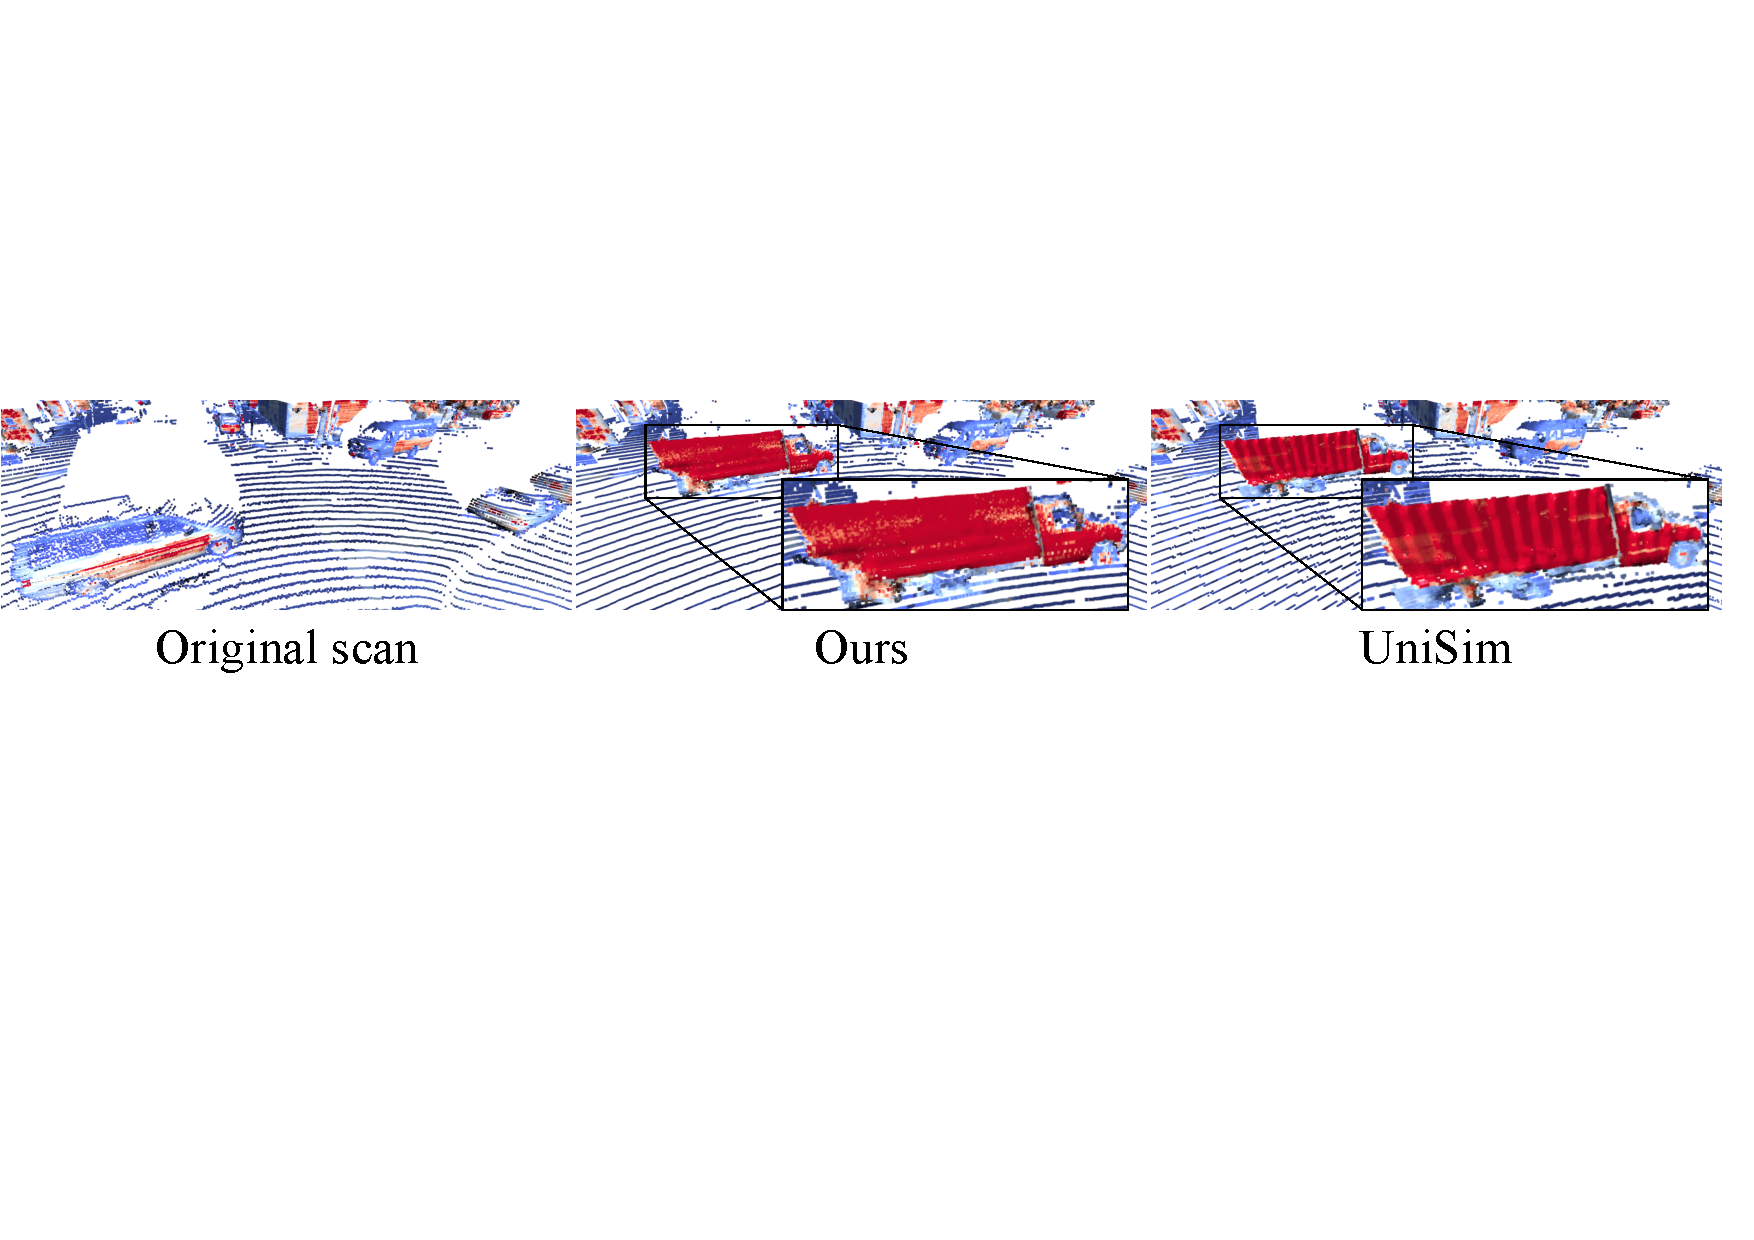
\includegraphics[width=1.0\linewidth]{Figures/vehicle_insertion.pdf}
    
    \caption{
    Qualitative results of object removal and insertion. \dynfl seamlessly inserts the neural asset (truck) into a new scene attributed to our superior compositional rendering scheme. In contrast, UniSim~\cite{yang2023unisim} struggles to accurately model geometry.
    }
    \label{fig:vehicle_insertion}
\end{figure}
\paragraph{Insert object from one scene into another}
Our explicit neural scene de-composition and flexible composition technique enable seamless insertion and removal of neural assets across scenes. As demonstrated in~\cref{fig:vehicle_insertion}, we are able to replace a car from one scene with a truck from another scene, achieving accurate reconstruction of both geometry and intensity. In contrast, UniSim~\cite{yang2023unisim} struggles to preserve high quality geometry. This highlights the significant potential of our approach in generating diverse and realistic LiDAR scans for autonomous driving scenarios.

\begin{figure}[t]
    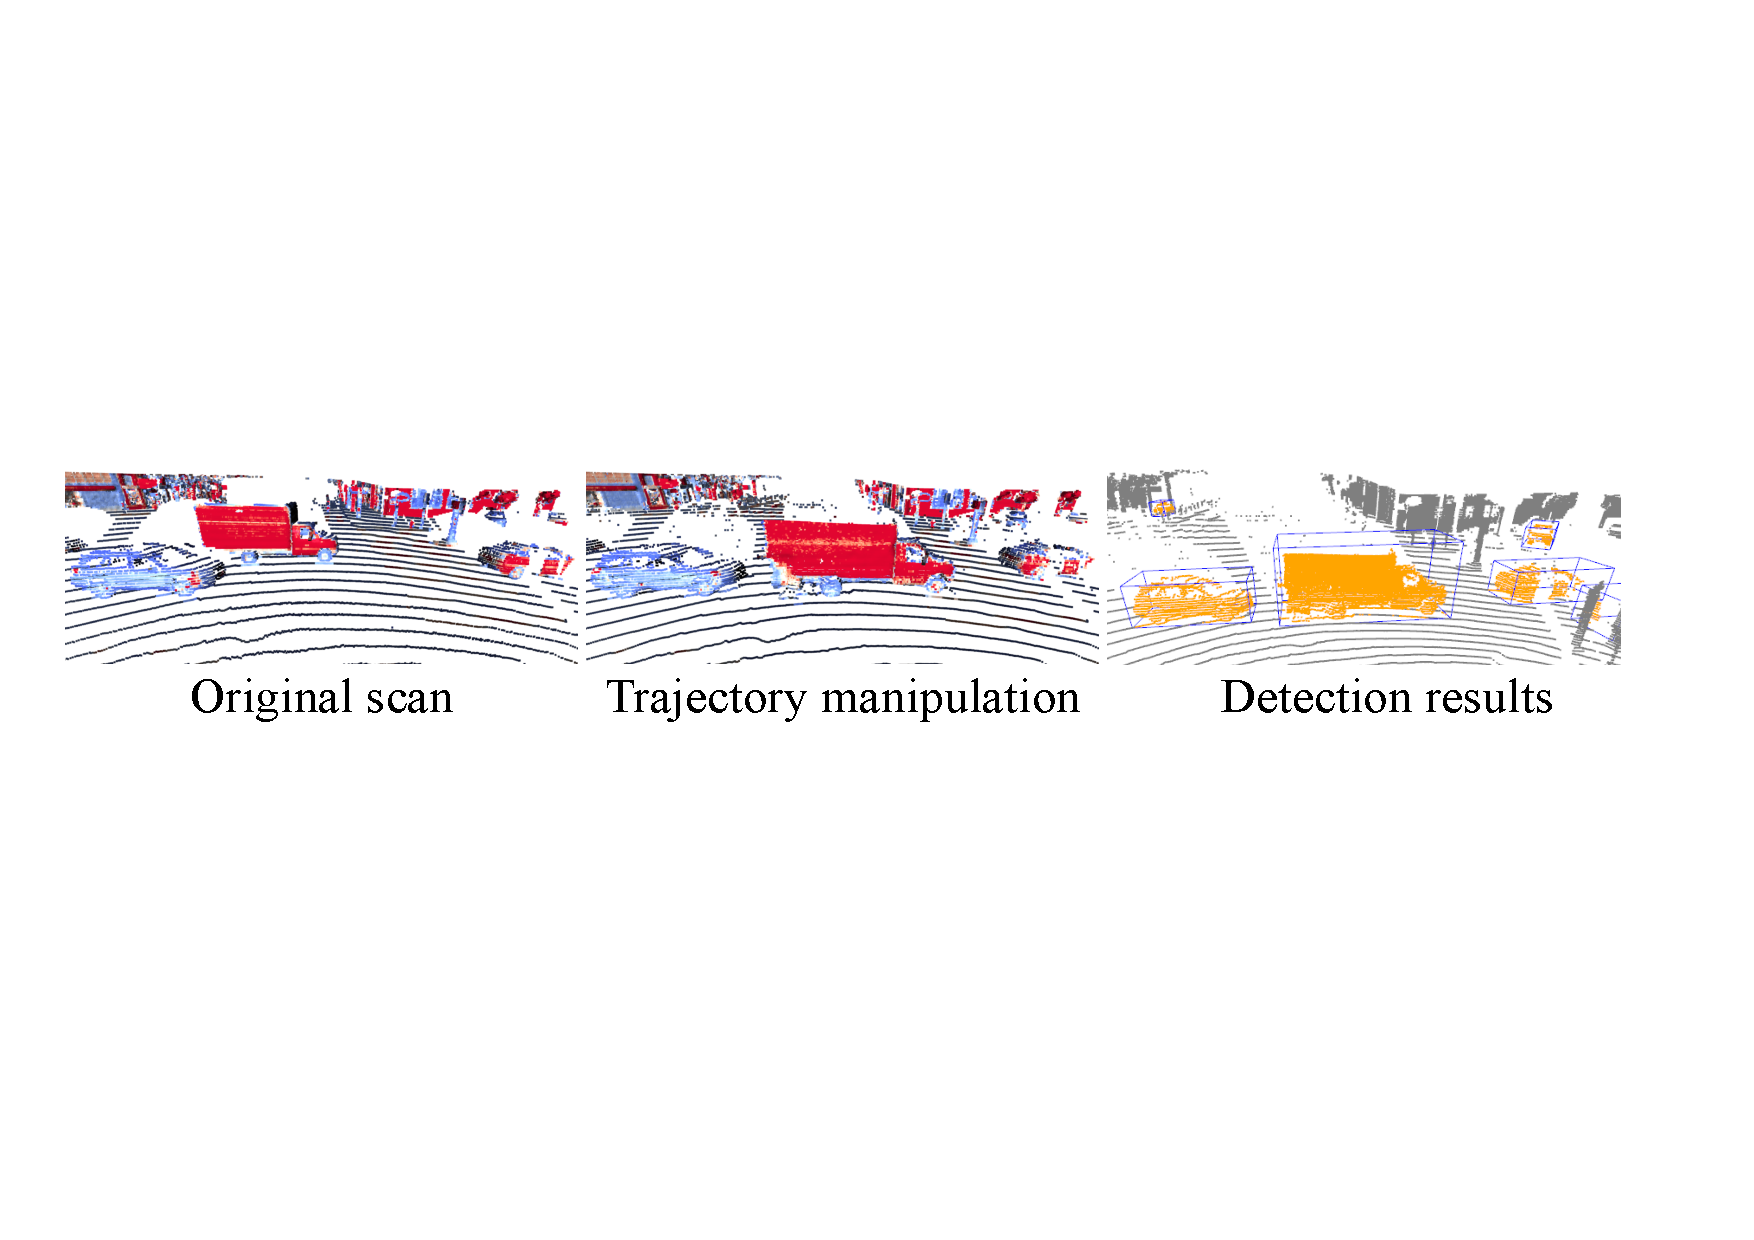
\includegraphics[width=1.0\columnwidth]{Figures/trajectory_manipulation.pdf}
    
    \caption{Qualitative results of object trajectory manipulation. The truck can be successfully detected after manipulation, indicating high-realism LiDAR re-simulation achieved by \dynfl.}
    \label{fig:traj}
    
\end{figure}
\paragraph{Manipulate the trajectory of dynamic objects}
\dynfl also facilitates the manipulation of moving objects' trajectories by simply adjusting their relative poses to the canonical bounding box. Representative results are shown in ~\cref{fig:traj}. The high realism of our re-simulation is also indicated by the successful detection of inserted virtual objects.

\section{Limitations and Future Work}
We present DyNFL, a compositional neural fields approach for LiDAR re-simulation. Our method excels previous art in both static and dynamic scenes, offering powerful scene editing capabilities that open up opportunities for generating diverse and high-quality scenes, to evaluate an autonomy system trained only on real data in closed-loop.

Despite achieving the state-of-the-art performance, there are still limitations we aim to address in future work. Firstly, \dynfl faces challenges in view synthesis of dynamic vehicles from unseen angles. This difficulty arises from the complexity of creating an a-priori model that can accurately complete unseen regions and simulate point cloud noise, ray drops patterns etc. Secondly, our method currently relies on object detection and tracking annotations, and its performance may be compromised when given inaccurate labels. Overcoming this dependency, exploring 4D representations while retaining scene editing flexibility, stands out as a crucial challenge for future research.


\paragraph{Acknowledgements.}
{Or Litany is a Taub fellow and is supported by the Azrieli Foundation Early Career Faculty Fellowship.}

\clearpage
\section{Appendix}
In this supplementary material, we first provide additional information about the datasets for our evaluations and implementation details of our proposed method in~\cref{sec:sup_dataset}. Next, we present more qualitative results in~\cref{sec:sup_visual}. Please also check the supplemental video for more results showcasing our performance. Finally, we provide the complete derivations of the SDF-based volume rendering for active sensor in~\cref{sec:sup_sdf_vol_render}. 

\section{Datasets and implementation details}\label{sec:sup_dataset}
\subsection{Datasets}
\paragraph{\textit{Waymo Dynamic}} For the \textit{Waymo Dynamic} dataset, we take them from 4 scenes of \textit{Waymo Open Dataset}~\cite{sun2020scalability}. There are multiple moving vehicles inside each scene. 50 consecutive frames are taken from each scene for our evaluation. The vehicles are deemed as \textit{dynamic} if the speed is $>1\,$m/s. in any of the 50 frames. The corresponding scene IDs on \textit{Waymo Open Dataset} for our selected scenes are shown as follows:
\begin{table}[!h]
    \setlength{\tabcolsep}{4pt}
    \renewcommand{\arraystretch}{1.2}
	\centering
	\resizebox{0.8\columnwidth}{!}{
    \begin{tabular}{l|c}
    \toprule
    & Scene ID \\
    \midrule
    Scene 1 & 1083056852838271990\_4080\_000\_4100\_000 \\
    Scene 2 & 13271285919570645382\_5320\_000\_5340\_000 \\
    Scene 3 & 10072140764565668044\_4060\_000\_4080\_000 \\
    Scene 4 & 10500357041547037089\_1474\_800\_1494\_800 \\
    \bottomrule
    \end{tabular}
    }
\end{table}

\subsection{Implementation details}
\paragraph{Ours} 
Our model is implemented based on nerfstudio\cite{nerfstudio}. For the static neural field, we sample $N_s=512$ points in total, with $N_u=256$ uniformly sampled points and $N_i=256$ weighted sampled points with 8 upsample steps. In each upsample step, 32 points are sampled based on the weight distribution of the previously sampled points. For each dynamic neural field, we sample $N_s=128$ points in total, with $N_u=64$ uniformly sampled points and $N_i=64$ weighted sampled points with 4 upsample steps. During training, we minimize the loss function using the Adam~\cite{kingma2014adam} optimiser, with an initial learning rate of 0.005. It linearly decays to 0.0005 towards the end of training. For the loss weights, we use $w_{\zeta}=3, w_{e}=50, w_{\text{drop}}=0.15, w_{s}=1$, and  $w_{\text{eik}}=0.3$. The batch size is 4096 and we train the model for 60000 iterations on a single RTX3090 GPU with float32 precision.

\paragraph{LiDARsim} We re-implement the LiDARsim~\cite{manivasagam2020lidarsim} as one of our baselines. 
First, we estimated point-wise normal vectors by considering all points within a 20 cm radius ball within the training set. Following this, we applied voxel down-sampling~\cite{tang2022torchsparse}, employing a 4 cm voxel size to reconstruct individual disk surfels at each point. The surfel orientation is defined based on the estimated normal vector. During inference, we apply the ray-surfel intersections test to determine the intersection points, thus the range and intensity values. We select a fixed surfel radius of 6 cm for the \textit{Waymo} dataset and 12 cm for the \textit{Town} dataset.
To handle dynamic vehicles, we follow LiDARsim~\cite{manivasagam2020lidarsim} by aggregating the LiDAR points for each vehicle from all the training frames and representing them in the \textit{canonical} frame of each vehicle. During inference, we transform all the aggregated vehicle points from their \textit{canonical} frames to the world frame and run ray-surfel intersection.

\paragraph{UniSim} 
We re-implement UniSim's~\cite{yang2023unisim} rendering process for LiDAR measurements by replacing our ray-drop test-based neural fields composition method with its joint rendering method. For every ray $\mathbf{r} (\mathbf{o},\mathbf{d})$, we begin by conducting an intersection test with all dynamic bounding boxes in the scene to identify the near and far limits. We then uniformly sample 512 points along each ray, assigning each point to either a dynamic neural field, if it falls within a dynamic bounding box, or to the static neural field otherwise. After sampling, we query the SDF and intensity values from the relevant neural fields. Finally, using the SDF-based volume rendering formula in Eq.~\ref{eq:depth_render} for active sensors, we calculate the weights and perform the rendering. Note that we use the same neural field architecture as in our method.
\begin{figure*}[t!]
  \centering
   \includegraphics[width=1\textwidth]{Figures_sup/4_scenes_sup.pdf}
   \caption{Visualization of 4 selected scenes from \textit{Waymo Dynamic} dataset. For each scene, we aggregate 50 frames. In the first row, points are color-coded by the intensity values(0 ~\bwrDyNFL~ 0.25). In the second row, dynamic vehicles are painted as \textcolor{yellow}{yellow}.}
   \label{fig:4_scenes_supp}
\end{figure*}

\begin{figure*}[t!]
  \centering
   \includegraphics[width=1\textwidth]{Figures_sup/supp_scene_edit.pdf}
   \caption{Visualization of scene editing capabilities. We showcase 3 kinds of scene editing capabilities including vehicle removal(left), trajectory manipulation(middle) and vehicle insertion(right). The first row represents the original scenes, the second row demonstrates the scenes after editing. All points are color-coded by the intensity values(0 ~\bwrDyNFL~ 0.25).}
   \label{fig:scene_editing_supp}
\end{figure*}

\section{More qualitative results}\label{sec:sup_visual}
In this section, we provide more qualitative results. In \cref{fig:4_scenes_supp}, we showcase the 4 scenes from \textit{Waymo dynamic} dataset. We show additional scene editing results in~\cref{fig:scene_editing_supp}. Please check the supplementary videos for more qualitative results.

\clearpage
\clearpage
\section{SDF-based volume rendering for active sensor}\label{sec:sup_sdf_vol_render}
In this section, we start by introducing the preliminary of NeRF~\cite{mildenhall2020nerf} following terminology as described in~\cite{tagliasacchi2022volume}. Then we provide the full derivation of the SDF-based volume rendering for active sensor. 

\subsection{Preliminary}\label{sec:supp_pre}
\paragraph{Density}
For a ray emitted from the origin $\origin \in \real^3$ towards direction $\dir \in \real^3$, the \textit{density} $\density_\zeta$ at range $\zeta$ indicates the likelihood of light interacting with particles at that point $\ray_\zeta = \origin + \zeta \dir$. This interaction can include absorption or scattering of light. In passive sensing, density $\density$ is a critical factor in determining how much light from the scene's illumination is likely to reach the sensor after passing through the medium.
\paragraph{Transmittance} quantifies the likelihood of light traveling through a given portion of the medium without being scattered or absorbed. Density is closely tied to the transmittance function $\transmittance(\zeta)$, which indicates the probability of a ray traveling over the interval $[0, \zeta)$ without hitting any particles. Then the probability $\transmittance(\zeta {+} d\zeta)$ of \emph{not} hitting a particle when taking a differential step $d\zeta$ is equal to $\transmittance(\zeta)$, the likelihood of the ray reaching $\zeta$, times $(1 - d\zeta \cdot \density(\zeta))$, the probability of not hitting anything during the step:
% 
\begin{align}
\transmittance(\zeta+d\zeta) =& \transmittance(\zeta) \cdot (1 - d\zeta \cdot \density(\zeta))
\\
\frac{\transmittance(\zeta+d\zeta) - \transmittance(\zeta)}{d\zeta} \equiv& \transmittance'(\zeta) = -\transmittance(\zeta) \cdot \sigma(\zeta) 
\label{eq:derivative}
\end{align}
% 
We solve the differential equation as follows:
%
\begin{align}
\transmittance'(\zeta) &= -\transmittance(\zeta) \cdot \density(\zeta) \\
\frac{\transmittance'(\zeta)}{\transmittance(\zeta)} &= -\density(\zeta) \\
\int_a^b \frac{\transmittance'(\zeta)}{\transmittance(\zeta)} \; d\zeta &= -\int_a^b \density(\zeta) \; d\zeta \\
\left. \log \transmittance(\zeta) \right|_a^b &= -\int_a^b \density(\zeta) \; d\zeta \\
\transmittance(a \rightarrow b) \equiv \frac{\transmittance(b)}{\transmittance(a)} &= \exponential{-\int_a^b \density(\zeta) \; d\zeta}   
\end{align}
% 
Hence, for a ray segment between $\zeta_0$ and $\zeta$, transmittance is given by:

\begin{equation}
\transmittance_{\zeta_0 \rightarrow \zeta} \equiv \frac{\transmittance_{\zeta}}{\transmittance_{\zeta_0}} = exp({-\int_{\zeta_0}^\zeta \density_t dt})\;,
\label{eq:trans_ab}
\end{equation}
which leads to following factorization of the transmittance:
\begin{equation}
\transmittance_{\zeta} = \transmittance_{0 \rightarrow \zeta_0} \cdot \transmittance_{\zeta_0 \rightarrow \zeta}\;.
\label{eq:factor}
\end{equation}

\paragraph{Opacity}Opacity is the complement of transmittance and represents the fraction of light that is either absorbed or scattered in the medium. In a homogeneous medium with constant density $\density$  the opacity for a segment $[\zeta_j, \zeta_{j+1}]$ of length $\Delta \zeta$ is given by $\opacity_{\zeta_j} = 1 - exp(-\density \cdot \Delta \zeta)$
\subsection{SDF-based volume rendering for active sensor}\label{sec:sdf_active}
NeuS\cite{wang2021neus} derives the opaque density based on the SDF which is:
\begin{equation}
\begin{split}
\density_{\zeta_i} =&  \max\left(\frac{-\frac{d\Phi_s}{d\zeta_i}(f(\zeta_i))}{\Phi_s(f(\zeta_i))},0\right)\\
                  =& \max\left(\frac{-(\nabla f(\zeta_i)\cdot \mathbf{v})\phi_s(f(\zeta_i))}{\Phi_s(f(\zeta_i))}, 0\right)
\end{split}
\label{eq:sigmoid_density}
\end{equation}
where $\Phi_s$ represents the Sigmoid function, $f$ is the SDF function that maps a range $\zeta$ to the SDF value of the point position $\origin + \dir * \zeta$. Note that the integral term is computed by
\begin{equation}
\int \frac{-(\nabla f(\zeta)\cdot \mathbf{v})\phi_s(f(\zeta))}{\Phi_s(f(\zeta))}d\zeta = -\ln(\Phi_s(f(\zeta))) + C,
\label{eq:intergration_density}
\end{equation}
% We can then calculate the accumulated transmittance from \ref{eq:trans_ab} using \ref{eq:intergration_density}:
% % 
% \begin{align}
% \transmittance_\zeta = \transmittance(0 \rightarrow \zeta) 
% % &= \prod_{k=1}^{n-1} \transmittance(t_k \rightarrow t_{k+1}) 
% &= \exponential{- \int_{0}^{\zeta} \density(t) \; dt} 
% = \Phi_s(f(\zeta))
% \label{eq:trans_const}
% \end{align}
We extend the density-based volume rendering for active sensor to SDF-based. Starting from the passive SDF-based volume rendering \cite{wang2021neus}, We substitute the density $\tilde{\density}$ with opaque density in \ref{eq:sigmoid_density}
and evaluate the radiant power integrated from ray segment [a,b] with constant reflectivity $\reflectivity_a$.

Consider the case where $-(\nabla f(\zeta)\cdot \mathbf{v})>0$ within the ray segment $[a,b]$, we have
\begin{align}
P(a \rightarrow b)
&= \int_a^b \transmittance^2(a\rightarrow t) \cdot \tilde{\density}_t \cdot \reflectivity(t)  \; dt
\\
&= \reflectivity_a \int_a^b \transmittance^2(a\rightarrow t) \cdot \tilde{\density}_t \; dt
\\
&= \reflectivity_a \int_a^b \exponential{-\int_a^t 2\tilde{\density}(u) \; du} \cdot \tilde{\density}_t \; dt
\\
&= \reflectivity_a \int_a^b \exponential{-2\int_a^t \tilde{\density}(u) \; du} \cdot \tilde{\density}_t \; dt
\\
&= \reflectivity_a \int_a^b \exponential{\left. 2\ln(\Phi_s(f(u)))\right|_a^t} \cdot \tilde{\density}_t \; dt
\\
% &= \reflectivity_a \int_a^b \exponential{2\ln(\Phi_s(f(t))) - 2\ln(\Phi_s(f(a)))} \cdot \tilde{\density}_t \; dt \\
&= \reflectivity_a \int_a^b \exponential{2\ln(\Omega_t) - 2\ln(\Omega_a)} \cdot \tilde{\density}_t \; dt 
\\
&= \reflectivity_a \int_a^b \frac{{\Omega_t}^2}{{\Omega_a}^2} \cdot \tilde{\density}_t \; dt ~~~~\text{\textbf{let} $\Omega_x = \Phi_s(f(x))$}
\\
&= \frac{\reflectivity_a}{{\Omega_a}^2} \int_a^b {\Omega_t}^2 \cdot \tilde{\density}_t \; dt 
\\
&= \frac{\reflectivity_a}{{\Omega_a}^2} \int_a^b -\frac{d\Phi_s}{dt}(f(t)) \cdot \Phi_s(f(t)) \; dt 
% \quad \text{$\tilde{\density}_t = \frac{-\frac{d\Phi_s}{d t}(f(t))}{\Phi_s(f(t))}$}
\\
&= \frac{\reflectivity_a}{{\Omega_a}^2} ( \left. -\frac{1}{2}{\Phi_s(f(t))}^2 \right|_a^b) \\
&= \frac{\reflectivity_a}{{\Omega_a}^2} (\frac{1}{2}{\Phi_s(f(a))}^2 -\frac{1}{2}{\Phi_s(f(b))}^2 )\\
&= \frac{{\Phi_s(f(a))}^2 -{\Phi_s(f(b))}^2}{{2\Phi_s(f(a))}^2} \cdot \reflectivity_a 
% \quad \text{$T_a$ = $\Phi_s(f(a))$}
\label{eq:homogeneous}
\end{align}
%\cref{eq:trans_const}

Consider the case where $-(\nabla f(\zeta)\cdot \mathbf{v})<0$ within the ray segment $[a,b]$, we have
\begin{align}
P(a \rightarrow b)
&= \int_a^b \transmittance^2(a\rightarrow t) \cdot \tilde{\density}_t \cdot \reflectivity(t)  \; dt
\\
&= \int_a^b \transmittance^2(a\rightarrow t) \cdot 0 \cdot \reflectivity(t)  \; dt
\\
&= 0
\end{align}
Hence we conclude 
\begin{align}
P(a \rightarrow b)
&= \max\left(\frac{{\Phi_s(f(a))}^2 -{\Phi_s(f(b))}^2}{{2\Phi_s(f(a))}^2},0\right) \cdot \reflectivity_a 
\end{align}

\paragraph{Volume rendering of piecewise constant data}
Combining the above, we can evaluate the volume rendering integral through a medium with piecewise constant reflectivity:
% 
\begin{align}
P(\zeta_{N+1}) &= \sum_{n=1}^N \int_{\zeta_n}^{\zeta_{n+1}} \transmittance^2(\zeta) \cdot \tilde{\density}_{\zeta} \cdot \reflectivity_{\zeta_n} \; d\zeta
\\
&= \sum_{n=1}^N \int_{\zeta_n}^{\zeta_{n+1}} \transmittance^2_{\zeta_n} \cdot \transmittance^2(\zeta_n \shortto \zeta) \cdot \tilde{\density}_{\zeta} \cdot \reflectivity_{\zeta_n} \; d\zeta 
% &&\text{from \ref{eq:factor}}
\\
&= \sum_{n=1}^N \transmittance^2_{\zeta_n}  \int_{\zeta_n}^{\zeta_{n+1}} \transmittance^2(\zeta_n \rightarrow \zeta) \cdot \tilde{\density}_{\zeta} \cdot \reflectivity_{\zeta_n} \; d\zeta \\
% &&\text{constant}
% \\
&=\sum_{n=1}^N \transmittance^2_{\zeta_n} P(\zeta_n \rightarrow \zeta_{n+1})
\\
&= \sum_{n=1}^N \transmittance^2_{\zeta_n} \cdot \tilde{\weight}_{\zeta_n} \cdot \reflectivity_{\zeta_n},
% &&\text{from \ref{eq:homogeneous}}
\end{align}

where 
\begin{align}
\tilde{\weight}_{\zeta_n} \equiv \max\left(\frac{{\Phi_s(f(\zeta_n)}^2 -{\Phi_s(f(\zeta_{n+1}))}^2}{{2\Phi_s(f(\zeta_n))}^2},0\right)
\end{align}
% 
% This leads to the volume rendering equations from NeRF~\cite[Eq.3]{mildenhall2020nerf}:
% % 
% \begin{align}
% P(\zeta_{N+1}) = \sum_{n=1}^N \transmittance^2_{\zeta_n} \cdot \frac{{\Phi_s(f(\zeta_n))}^2 -{\Phi_s(f(\zeta_{n+1}))}^2}{{2\Phi_s(f(\zeta_n))}^2} \cdot \reflectivity_{\zeta_n}
% \label{eq:final_radiant}
% \end{align}
% % 
% Since the opacity is always greater than 0, we can express the opacity as
% \begin{equation}
%     \tilde{\weight}_{\zeta_n} \equiv max(\frac{{\Phi_s(f(\zeta_n))}^2 -{\Phi_s(f(\zeta_{n+1}))}^2}{{2\Phi_s(f(\zeta_n))}^2}, 0)
%     \label{eq:opacity}
% \end{equation}

The discrete accumulated transmittance $\transmittance$ can be calculated as follows:

Consider the case where $-(\nabla f(\zeta)\cdot \mathbf{v}) > 0$ in $[\zeta_n, \zeta_{n+1}]$: 
%
\begin{align}
\transmittance_{\zeta_n} 
&=\prod_{i=1}^{n-1}(\exp(-\int_{\zeta_n}^{\zeta_{n+1}}\tilde{\density}_\zeta \; d\zeta) \\
&= \prod_{i=1}^{n-1}(\frac{\Phi_s(f(\zeta_{n+1}))}{\Phi_s(f(\zeta_n))})\\
\transmittance^2_{\zeta_n}
&= \prod_{i=1}^{n-1}(\frac{{\Phi_s(f(\zeta_{n+1}))}^2}{{\Phi_s(f(\zeta_n))}^2})\\
&= \prod_{i=1}^{n-1}(1-2\tilde{\weight}_{\zeta_n})
\label{eq:dicrete_transmittance}
\end{align}

Consider the case where $-(\nabla f(\zeta)\cdot \mathbf{v}) < 0$ in $[\zeta_n, \zeta_{n+1}]$: 
\begin{align}
\transmittance_{\zeta_n} 
&=\prod_{i=1}^{n-1}(\exp(-\int_{\zeta_n}^{\zeta_{n+1}}\tilde{\density}_\zeta \; d\zeta) = \prod_{i=1}^{n-1}(1)
\\
\transmittance^2_{\zeta_n} &= \prod_{i=1}^{n-1}(1^2) = \prod_{i=1}^{n-1}(1-2\tilde{\weight}_{\zeta_n})
\end{align}
In conclusion, the radiant power can be reformulated as:

\begin{align}
P(\zeta_{N+1}) = \sum_{n=1}^N \transmittance^2_{\zeta_n} \cdot \tilde{\weight}_{\zeta_n} \cdot \reflectivity_{\zeta_n}
\label{eq:final_radiant2}
\end{align}
where $\transmittance^2_{\zeta_n} = \prod_{i=1}^{n-1}(1-2\tilde{\weight}_{\zeta_i})$


\paragraph{Depth volume rendering of piecewise constant data}

Note that $\tilde{\weight}_{\zeta_n} \in [0, 0.5], \transmittance^2_{\zeta_n} \in [0,1], \sum_{n=1}^N \transmittance^2_{\zeta_n} \cdot \tilde{\weight}_{\zeta_n} = 0.5$, for depth volumetric rendering, we have 
\begin{align}
    \zeta = \sum_{n=1}^N 2 \cdot \transmittance^2_{\zeta_n} \cdot \tilde{\weight}_{\zeta_n} \cdot \zeta_n
    =\sum_{n=1}^N w_n \cdot \zeta_n
    \label{eq:depth_render}
\end{align}
where $w_n = 2\tilde{\weight}_{\zeta_n} \cdot \prod_{i=1}^{n-1}(1-2\tilde{\weight}_{\zeta_i})$

\renewcommand{\subdir}{tex/ECCV2022_PCAccumulation}
\chapter[Dynamic LiDAR Re-simulation using Compositional Neural Fields]{Dynamic LiDAR Re-simulation using Compositional Neural Fields}
\label{chap:cvpr24}

Hanfeng Wu, Xingxing Zuo, Stefan Leutenegger, Or Litany, Konrad Schindler, Shengyu Huang \\
\textbf{IEEE/CVF Conference on Computer Vision and Pattern Recognition, 2024}\\
\\
(Author version; for typeset version please refer to the original conference paper.)\\

\providecommand{\subdir}{.}
\graphicspath{{\subdir/}}

\section*{Abstract}
We present Neural Fields for LiDAR (NFL), a method to optimise a neural field scene representation from LiDAR measurements, with the goal of synthesizing realistic LiDAR scans from novel viewpoints. 
NFL combines the rendering power of neural fields with a detailed, physically motivated model of the LiDAR sensing process, thus enabling it to accurately reproduce key sensor behaviors like beam divergence, secondary returns, and ray dropping.
We evaluate NFL on synthetic and real LiDAR scans and show that it outperforms explicit reconstruct-then-simulate methods as well as other NeRF-style methods on LiDAR novel view synthesis task. Moreover, we show that the improved realism of the synthesized views narrows the domain gap to real scans and translates to better registration and semantic segmentation performance. Project page: \url{https://research.nvidia.com/labs/toronto-ai/nfl}.
\newpage
\section{Introduction}
\begin{figure*}[t]
    \centering
        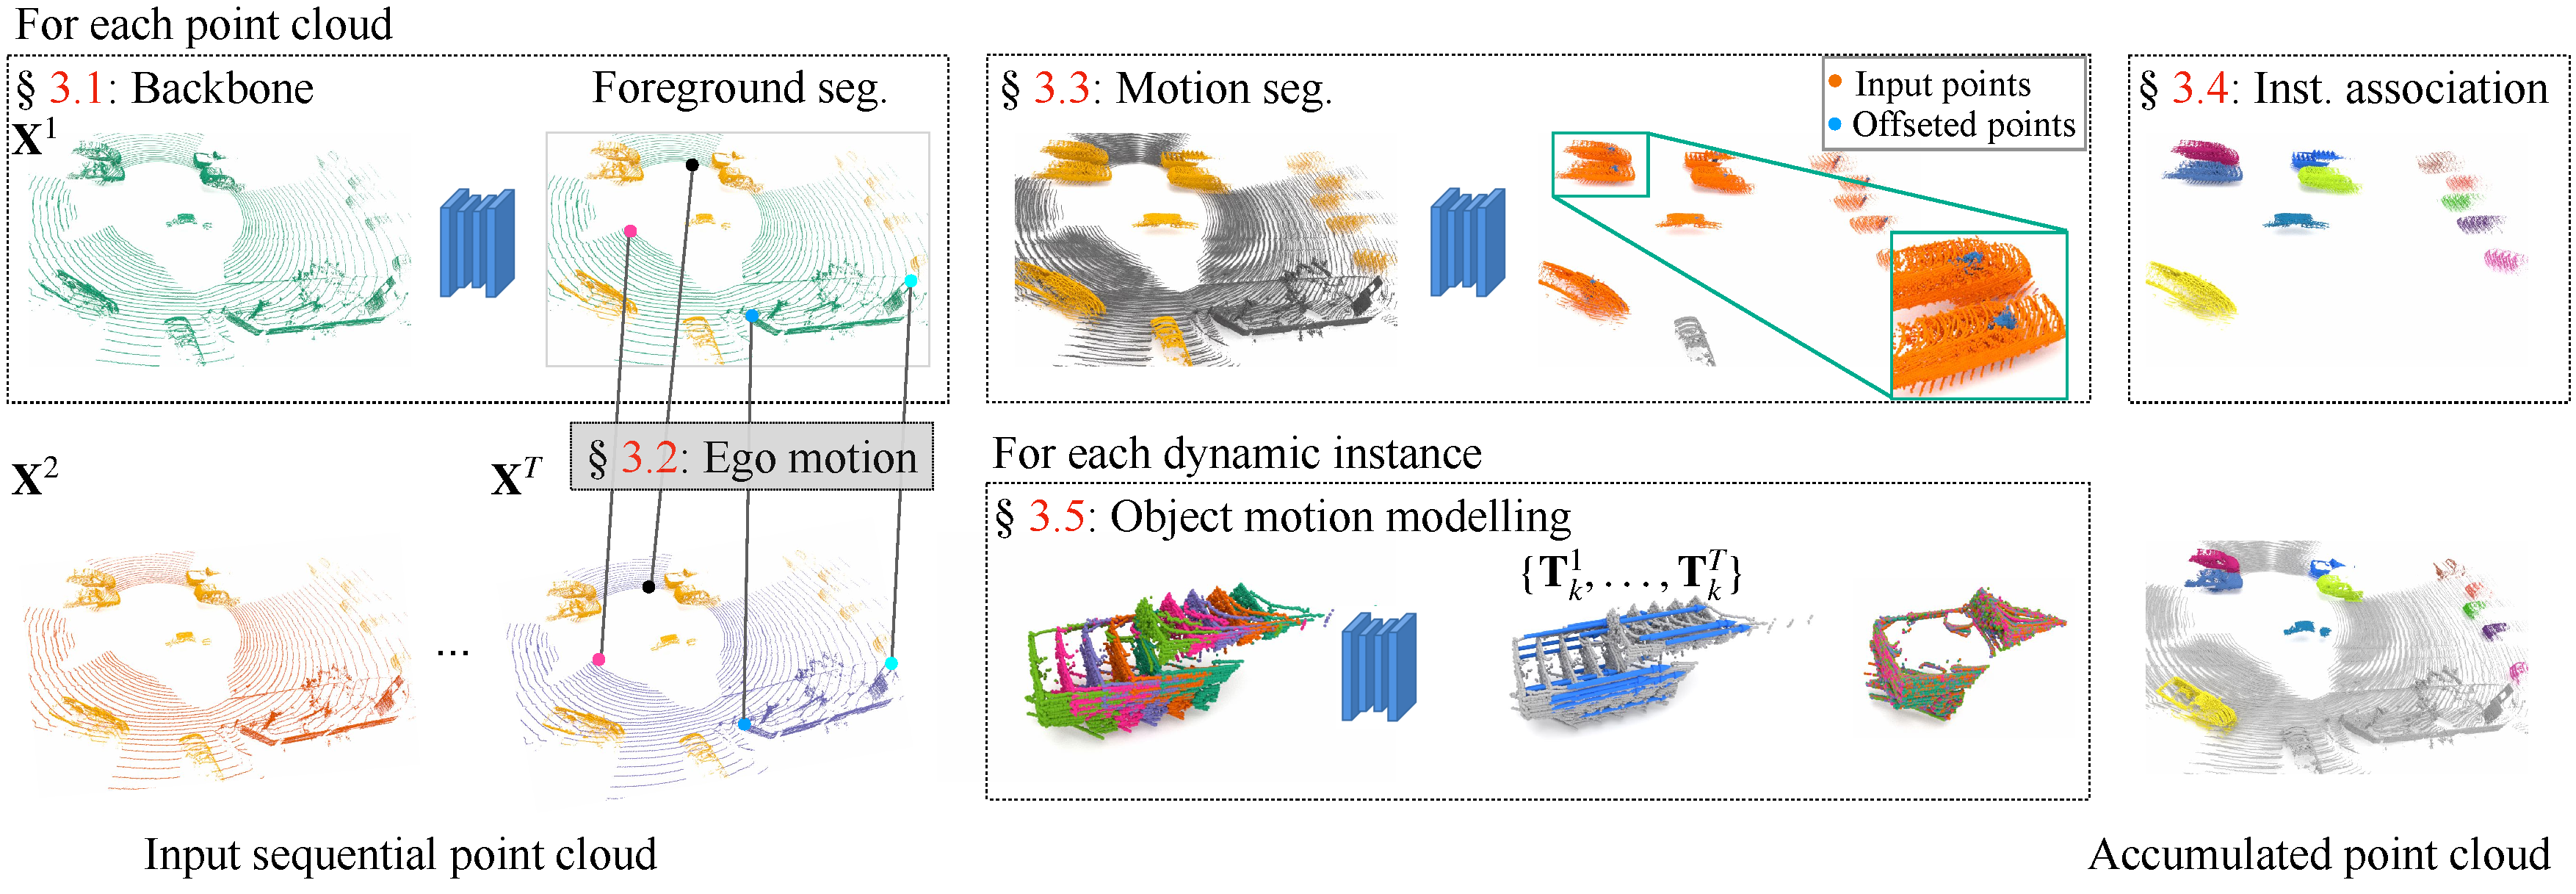
\includegraphics[width=1.0\textwidth]{Figures/overview.pdf}
        \caption{
        Overview of \dynfl. Our method takes LiDAR scans and tracked bounding boxes of dynamic vehicles as input. \dynfl first decomposes the scene into a static background and $N$ dynamic vehicles, each modelled using a dedicated neural field. These neural fields are then composed to re-simulate LiDAR scans in dynamic scenes. Our composition technique supports various scene edits, including altering object trajectories, removing and adding reconstructed neural assets between scenes.
    }
    \label{fig:main}
\end{figure*}

We introduce a neural representation for the purpose of reconstructing and manipulating LiDAR scans of dynamic driving scenes. 
Counterfactual re-simulation is an emerging application in the realm of autonomous driving, offering a unique approach to examining "what if" scenarios. This method involves creating a reconstruction of a real-world event, termed as \textit{digital twin} and then applying various modifications to it. These could include altering the environmental conditions, changing the action of some agent, or introducing additional scene elements. Analyzing the outcomes of these edited scenarios provides insights into the functioning of the perception system, moreover they can be used to obtain training data for rare situations.

The essence of counterfactual re-simulation is the capability to authentically recreate variations of the original, factual observation. We address this challenge in the context of LiDAR on autonomous vehicles (AV). Existing approaches to LiDAR re-simulation have important limitations. Conventional simulators such as CARLA~\cite{dosovitskiy2017carla} and NVIDIA DRIVE Sim are capable of modeling LiDAR sensors. However, their reliance on manually designed 3D simulation assets requires significant human effort. LiDARsim~\cite{manivasagam2020lidarsim} aims to remedy this by reconstructing vehicles and scenes from real measurements. While producing encouraging results, its two-stage LiDAR modeling lacks realism, particularly in terms of physical effects like multi-returns and reflected intensity, which were shown 
 to matter for downstream processing~\cite{guillard2022learning}. Following NeRF's~\cite{mildenhall2020nerf} success in camera view synthesis, some works have applied neural fields for LiDAR modeling~\cite{Huang2023nfl, tao2023lidar, zhang2023nerf}. In particular, Neural LiDAR Fields (NFL)\cite{Huang2023nfl} developed a physically inspired LiDAR volumetric rendering scheme that accounts for two-way transmittance and beam width, allowing faithful recovery of secondary returns, intensity, and ray drops. These models are, however, limited to static scenes that do not change while multiple input views are scanned, and are thus of limited use for re-simulation in the presence of moving traffic. Recently, UniSim~\cite{yang2023unisim} followed Neural Scene Graph~\cite{Ost_2021_CVPR} in modeling road scenes as sets of movable NeRF instances on top of a static background. UniSim introduced a unified synthesis approach for camera and LiDAR sensors, but ignored physical sensor properties like two-way transmittance and beam width~\cite{Huang2023nfl}.

We present \dynfl, a novel approach for re-simulating LiDAR views of driving scenarios. Our method builds upon a neural SDF that enables an accurate representation of scene geometry, while at the same time enforcing physical accuracy by modeling two-way transmittance, like NFL~\cite{Huang2023nfl}. 
% Our method builds upon UniSim's SDF representation and scene decomposition, but enhances the physical accuracy by incorporating two-way transmittance modeling, as introduced in NFL.
%
Our primary contribution is a method for compositing neural fields that accurately integrates LiDAR measurements from individual fields representing different scene assets. With the help of a ray drop test, we effectively manage occlusions and transparent surfaces. This not only ensures physical accuracy, but also facilitates the inclusion of assets reconstructed from a variety of static and dynamic scenes, thereby enhancing control over the simulated content. Our method bridges the gap between the physical fidelity of the re-simulation and flexible editing of dynamic scenes.
%
We validate \dynfl with both synthetic and real-world data, focusing on three key areas: \textit{(i)} high-quality view synthesis, \textit{(ii)} perceptual fidelity, and \textit{(iii)} asset manipulation. We find that our approach outperforms baseline models \wrt both range and intensity. Its synthetic outputs also show higher agreement with real scans in terms of object detection and segmentation. Furthermore, \dynfl enables not only removal, duplication and repositioning of assets within the same scene, but also the inclusion of assets reconstructed in other scenes, paving the way for new applications.


% In the rapidly evolving field of computer vision, novel view synthesis has become a groundbreaking technique, especially in the realm of image-based rendering. Pioneered by technologies like NeRF~\cite{mildenhall2020nerf}, it allows for the creation of photo-realistic views from a given set of data. However, the application of these principles to LiDAR data, which inherently deals with point clouds, introduces a complex set of challenges and opportunities that are distinct from traditional image-based approaches.

% Historically, methods like LiDARsim~\cite{manivasagam2020lidarsim} have paved the way for such advancements, yet they exhibit limitations. Specifically, LiDARsim operates by first extracting an explicit scene representation and then performing ray-surfel casting to synthesize LiDAR scans. This approach, while innovative, is susceptible to inaccuracies due to point cloud noise and typically results in lower reconstruction quality. This limitation leads to a significant domain gap when compared to ground truth LiDAR scans. Our previous work, Neural Lidar Fields (NFL)~\cite{Huang2023nfl}, marked a substantial improvement in modeling LiDAR scenes with neural fields and incorporating the physical characteristics of LiDAR beams. Despite its state-of-the-art performance in geometry reconstruction, NFL was limited to static scenes and did not address the complexities of dynamic environments.

% In dynamic scenarios, particularly in automotive or robotics contexts, capturing the constant motion of elements like vehicles and pedestrians is crucial. Our work seeks to bridge this gap by extending the principles of NFL to dynamic settings. Prior approaches that tackle the dynamic scenes, such as LiDARsim~\cite{manivasagam2020lidarsim}, have adopted a reconstruct-then-simulate process, resulting in inferior geometric fidelity. Meanwhile, other neural-fields-based explorations like Neural Scene Graph~\cite{Ost_2021_CVPR} and UniSim~\cite{yang2023unisim} focus on image-based rendering or sensor fusion, neglecting LiDAR-specific attributes.

% In this context, our work contributes in several ways:
% \textbf{1.)} Improved Geometry Quality: We adopt a Signed Distance Function (SDF)-based volume rendering approach, specifically tailored to the active sensor characteristics of LiDAR beam. This method acknowledges and leverages the intricacies of how LiDAR sensors capture data, resulting in reconstructions of higher fidelity and geometric accuracy.
% \textbf{2.)} Innovative Neural Fields Composition: Our methodology introduces a novel technique for the composition of multiple neural fields. This approach significantly enhances the rendering process, allowing for seamless integration and higher-quality synthesis of dynamic views.

% Our paper delves into the technicalities of Dynamic Neural LiDAR Fields, elaborating on the methods and innovations that enable the synthesis of dynamic views from LiDAR data. We present extensive experimental results that showcase the effectiveness of our approach in dynamic environments, illustrating how our contributions extend the applicability of neural LiDAR fields. Through this work, we provide a valuable resource for researchers in computer vision, contributing to the broader discourse on LiDAR novel view synthesis for dynamic scenes.


\section{Related work}
\paragraph{Neural radiance fields and volume rendering}
Neural Radiance Fields (NeRF)~\cite{mildenhall2020nerf} have demonstrated remarkable success in novel-view image synthesis through neural volume rendering. These fields are characterized by the weights of Multilayer Perceptrons (MLPs), which enable the retrieval of volume density and RGB colors at any specified point within the field for image compositing via volume rendering. Several studies~\cite{barron2021mip,barron2022mip,verbin2022ref,chen2022tensorf,fridovich2022plenoxels} have subsequently advanced NeRF's rendering quality by addressing challenges such as reducing aliasing artifacts~\cite{barron2021mip}, scaling to unbound large-scale scenarios~\cite{barron2022mip}, and capturing specular reflections on glossy surfaces~\cite{verbin2022ref}.
Certain works~\cite{chen2022tensorf,fridovich2022plenoxels,mueller2022instant,kerbl20233d} have explored more effective representations of radiance fields. TensorsRF~\cite{chen2022tensorf} employs multiple compact low-rank tensor components, such as vectors and matrices, to represent the radiance field. Plenoxels~\cite{fridovich2022plenoxels} accelerates NeRF training by replacing MLPs with explicit plenoptic elements stored in sparse voxels and factorizing appearance through spherical-harmonic functions.
M\"uller et al.~\cite{mueller2022instant} achieved a substantial acceleration in rendering speed by employing a representation that combines trainable multi-resolution hash encodings (MHE) with shared shallow MLP networks. Kerbel et al.~\cite{kerbl20233d} introduce a novel volume rendering method utilizing 3D Gaussians to represent the radiance field and rendering images based on visibility-aware splatting of 3D Gaussians.


\paragraph{Dynamic neural radiance fields} 
Neural fields \cite{xie2022neural} can be extended to represent dynamic scenes. On top of the \textit{canonical} scene representation, some methods~\cite{pumarola2020d, park2021nerfies, park2021hypernerf,yuan2021star} additionally model the 4D deformation fields. Meanwhile, some other works learn a space-time correlated~\cite{kplanes_2023, li2020neural, attal2023hyperreel, liu2023robust}, or decomposed~\cite{turki2023suds,wu2022d,yang2023emernerf} neural field to encode the 4D scenes, achieving fine-grained reconstruction of the geometry and the appearance.
%
Some other methods decompose the scene into static and dynamic parts, and model each dynamic actor with dedicated neural fields. 
Neural Scene Graph~\cite{Ost_2021_CVPR} and Panoptic Neural Fields~\cite{KunduCVPR2022PNF} treat every dynamic object in the scene as a node, and synthesize photo-realistic RGB images by jointly rendering from both dynamic nodes and static background. UniSim\cite{yang2023unisim} employs neural SDF representation to model dynamic scenes in driving scenarios, and render in a similar way to Neural Scene Graph~\cite{Ost_2021_CVPR}.


\paragraph{Neural surface representation}
A fundamental challenge for NeRF and its variants involves accurately recovering the underlying 3D surface from the implicit radiance field. Surfaces obtained by thresholding on the volume density of NeRF often exhibit noise~\cite{wang2021neus, yariv2021volume}. To address this, implicit surface representations like Occupancy~\cite{niemeyer2020differentiable, oechsle2021unisurf} and signed distance functions (SDF)~\cite{wang2021neus, yariv2021volume, yu2022monosdf, sun2022neural, wang2022hf, zuo2023incremental, li2023neuralangelo, wang2023neus2} in grid maps are commonly integrated into neural volume rendering techniques.

NeuS~\cite{wang2021neus} introduces a neural SDF representation for surface reconstruction, proposing an unbiased weight function for the appearance composition process in volume rendering. Similarly, VolSDF~\cite{yariv2021volume} models scenes with a neural SDF and incorporates the SDF into the volume rendering process, advocating a sampling strategy of the viewing ray to bound opacity approximation error. Neuralangelo~\cite{li2023neuralangelo} improves surface reconstruction using the multi-resolution hash encoding (MHE)~\cite{mueller2022instant} and SDF-based volume rendering~\cite{wang2021neus}. While these methods might deliver satisfying dense surface reconstructions, their training is time-consuming, taking hours for a single scene.
Voxurf~\cite{wu2022voxurf} offers a faster surface reconstruction method through a two-stage training procedure, recovering the coarse shape first and refining details later. Wang et al.~\cite{wang2023neus2} expedites NeuS training to several minutes by predicting SDFs through a pipeline composed of MHE and shallow MLPs.

Many works also incorporate distances measured by LiDAR as auxiliary information to constrain the radiance field. For instance, works~\cite{chang2023neural, wang2023neural} render depth by accumulating volume density and minimizing depth discrepancies between LiDAR and render depth during training. Rematas et al.~\cite{rematas2022urban} enforces empty space between the actual surface and the ray origin.


\paragraph{LiDAR simulation} 
While simulators like CARLA~\cite{dosovitskiy2017carla} and AirSim~\cite{shah2018airsim} can simulate LiDAR data, they suffer from expensive human annotation requirements and a notable sim-to-real gap due to limited rendering quality. Generative model-based methods for LiDAR synthesis~\cite{caccia2019deep,zyrianov2022learning} offer an alternative but often lack control and produce distorted geometries~\cite{li2023pcgen}.
Learning-based approaches~\cite{li2023pcgen,fang2020augmented,manivasagam2020lidarsim} try to enhance realism by transferring real scan properties to simulations. For example, \cite{guillard2022learning} uses a RINet trained on RGB and real LiDAR data to augment simulated scan qualities. LiDARsim~\cite{manivasagam2020lidarsim} employs ray-surfel casting with explicit disk surfels for more accurate simulations.
Huang et al.~\cite{Huang2023nfl} proposed Neural LiDAR Fields (NFL), combining neural fields with a physical LiDAR model for high-quality synthesis, although it's limited to static scenes and can produce noisy outputs due to its unconstrained volume density representation.
UniSim~\cite{yang2023unisim} constructs neural scene representations from realistic LiDAR and camera data, using SDF-based volume rendering for sensor measurement generation at novel viewpoints.


\section{Dynamic Neural Scene Representation}

\paragraph{Problem statement} 
Consider a set of LiDAR scans $\mathcal{X} = \{\mathbf{X}_t\}_{t=1}^T$ that have been compensated for ego-motion, along with tracked bounding boxes\footnote{We assume that the ground truth object detection and tracking annotations are available.} for dynamic vehicles $\mathcal{B} = \{\mathbf{B}_t^v\}_{v=1}^{N}$, where $T$ represents the total number of LiDAR scans, and $N$ is the count of dynamic vehicles. Each scan $\mathbf{X}_t$ is composed of $n_t$ rays, each ray $\mathbf{r}$ is described by the tuple $(\origin, \dir, \zeta, \intensity, \pdrop)$, where $\origin$ and $\dir$ denote the ray's origin and direction, $\zeta$ and $\intensity$ represent range and intensity values, and $\pdrop \in \{0,1\}$ indicates whether the ray is dropped or not due to insufficient returned radiant power.


The goal is to reconstruct the scene with a static-dynamic decomposed neural representation, that can enable the rendering of LiDAR scan $\mathbf{X}_{\text{tgt}}$ from novel viewpoint $\mathbf{T}_{\text{tgt}}$. This setup also facilitates various object manipulations, including altering object trajectories, and inserting or removing objects from the scene. The overview of our method is given in~\cref{fig:main}.

\subsection{Neural Scene Decomposition} \label{sec: decomposition}
We leverage the inductive bias that driving scenes can be decomposed into a static component and $N$ rigidly-moving dynamic components~\cite{huang2022dynamic,gojcic2021weakly}. Consequently, we establish $N+1$ neural fields. The neural field $\mathbf{F}_{\text{static}}$ is designated for the static component of the scene, capturing the unchanging background elements. Concurrently, the set of neural fields $\{\mathbf{F}^v\}_{v=1}^{N}$ is used to model the $N$ dynamic entities, specifically the vehicles in motion.



\paragraph{Neural field for static background} 
The static background is encoded into a neural field $\mathbf{F}_\text{static}: (\x, \dir) \mapsto (s, \intensity, \pdrop)$ that estimates the signed distance $s$, intensity $\intensity$, and ray drop probability $\pdrop \in [0,1]$ given the point coordinates $\x$ and the ray direction $\dir$. In practice, we first use a multi-resolution hash encoding (MRH)~\cite{mueller2022instant} to map each point to its positional feature $\posfeat \in \real^{32}$, and project the view direction onto the first 16 coefficients of the spherical harmonics basis, resulting in $\dirfeat$. Subsequently, we utilize three Multilayer Perceptrons (MLPs) to estimate the scene properties as follows:
\begin{equation}
(s, \geofeat) = f_s(\posfeat), \quad \intensity = f_{\intensity}(\rayfeat), \quad \pdrop = f_{\text{drop}}(\rayfeat).
\end{equation}
Here, $f_s, f_e,$ and $f_{\text{drop}}$ are three MLPs, $\rayfeat \in \mathbb{R}^{31}$ represents the ray feature and is constructed by concatenating the per-point geometric feature and the directional feature. The geometric feature is denoted as $\geofeat \in \mathbb{R}^{16}$. For more implementation details, please refer to the appendix. 

\begin{figure}[t]
    \centering
        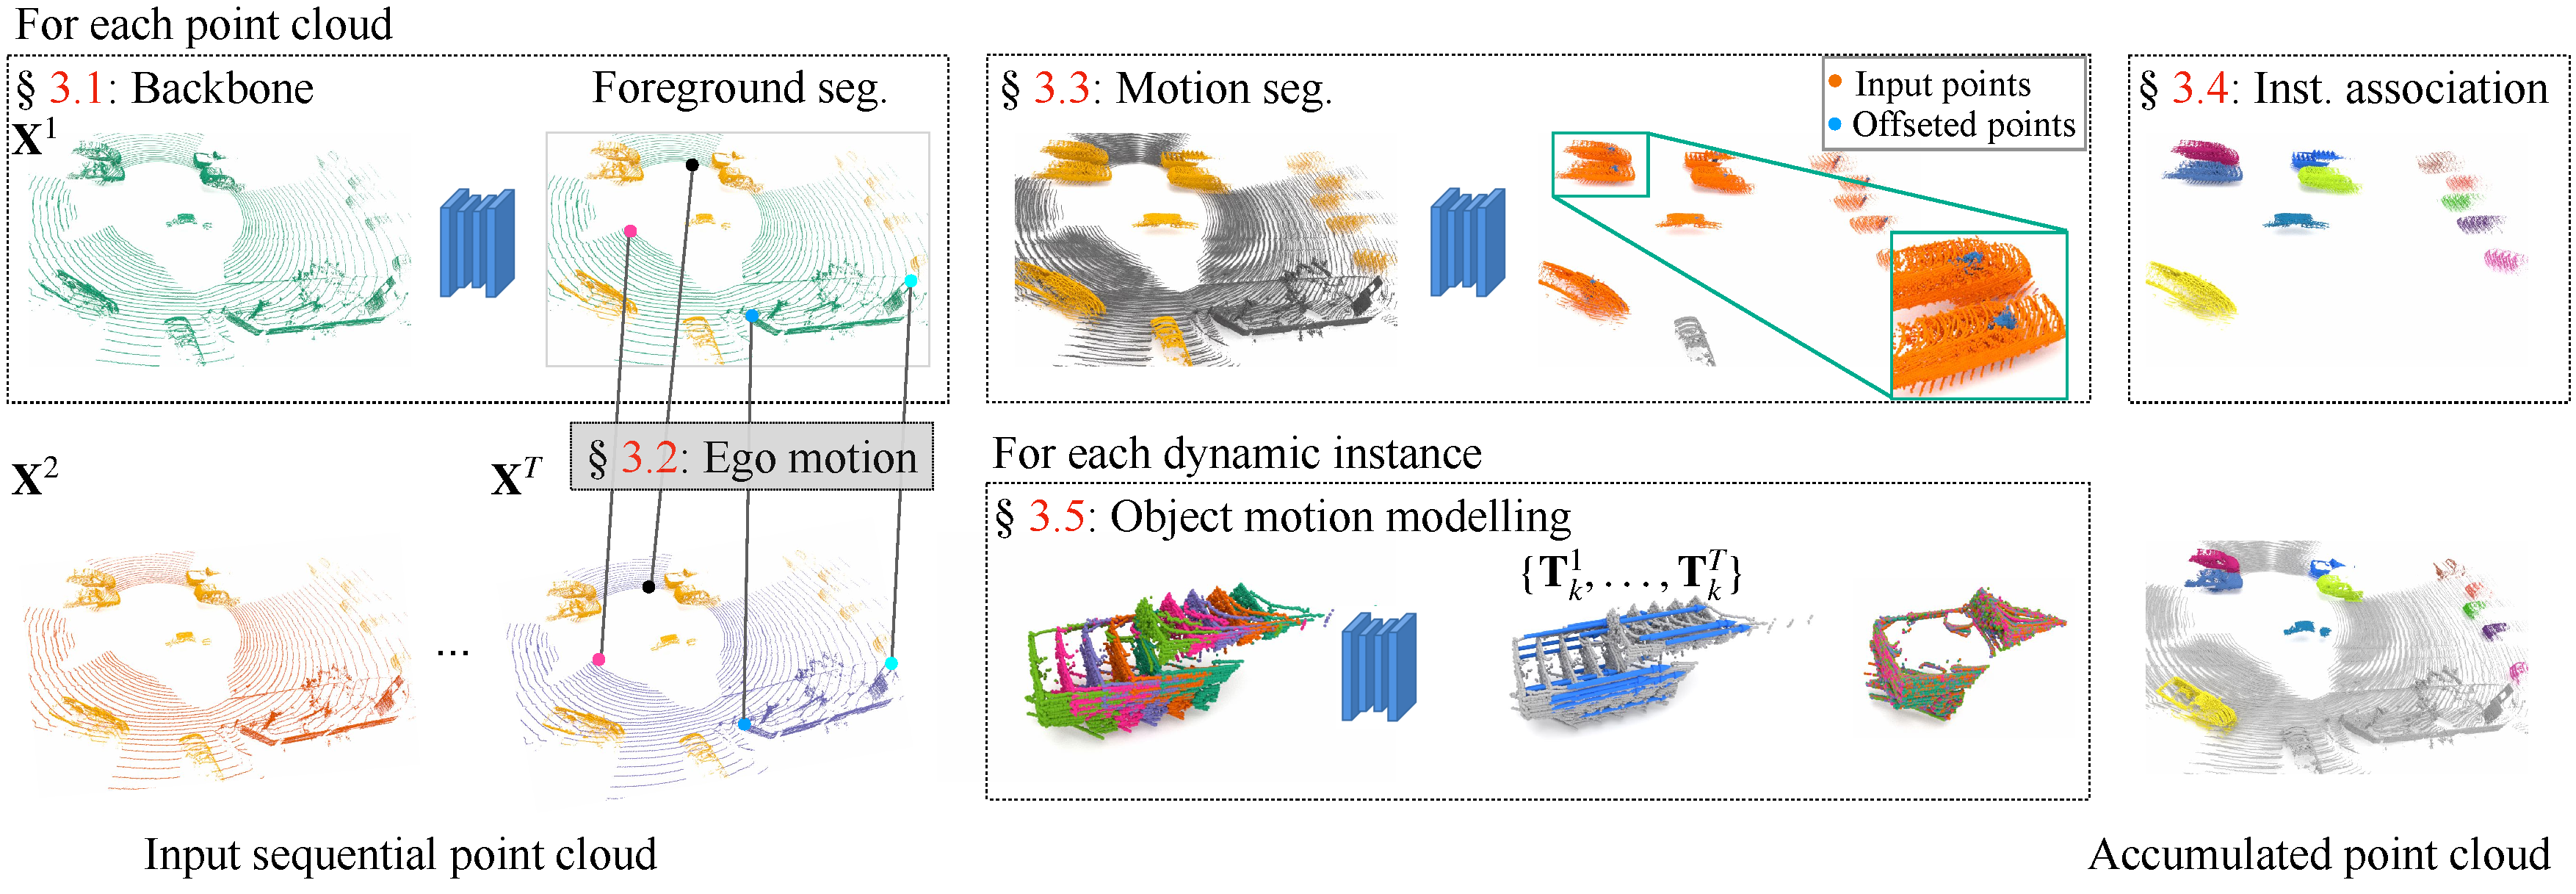
\includegraphics[width=1.0\columnwidth]{Figures/overview.pdf}
        \caption{
        Overview of \dynfl. Our method takes LiDAR scans and tracked bounding boxes of dynamic vehicles as input. \dynfl first decomposes the scene into a static background and $N$ dynamic vehicles, each modelled using a dedicated neural field. These neural fields are then composed to re-simulate LiDAR scans in dynamic scenes. Our composition technique supports various scene edits, including altering object trajectories, removing and adding reconstructed neural assets between scenes.
    }
    \label{fig:main}
\end{figure}


\paragraph{Neural fields for dynamic vehicles} 
LiDAR scans collected over time are often mis-aligned due to the motion of both the sensor and other objects in the scene. Despite applying ego-motion for aligning static background points, dynamic object points remain blurred along their trajectories. Our approach to constructing a dynamic neural scene representation is grounded in the assumption that each dynamic object only undergoes rigid motion. Therefore, we can first align them over time and reconstruct them in their \textit{canonical} coordinate frame, and then render them over time by reversing the alignment of the neural field.

Specifically, consider a dynamic vehicle $v$ 
occurring in LiDAR scans $\{\mathbf{X}^v_t\}_{t=1}^{T}$ along with the associated bounding boxes $\{\mathbf{B}^v_t \in \mathbb{R}^{3\times 8}\}_{t=1}^{T}$ in the world coordinate framework. Here each bounding box is defined by its eight corners, and the first bounding box $\mathbf{B}^v_1$ is considered as the \textit{canonical} box. We estimate the relative transformations $\{\mathbf{T}_t \in \text{SE}(3)\}_{t=2}^{T}$ between the remaining $T-1$ bounding boxes and the canonical box, expressed as $\mathbf{B}_1^v = \mathbf{T}_t \mathbf{B}_t^v$\footnote{$\mathbf{T}\mathbf{B} = \mathbf{R}\mathbf{B} + \mathbf{t}$, where $\mathbf{R}$ and $\mathbf{t}$ are the rotation and translation components of $\mathbf{T}$.}. 
Subsequently, all LiDAR measurements on the object are transformed and accumulated in its canonical coordinate frame. The vehicle $v$ is then reconstructed in its canonical space, akin to the static background, using a neural field $\mathbf{F}^v$. To render the dynamic vehicle at timestamp $t$, the corresponding rigid transformation is applied to the queried rays. The dynamic neural field can thus be expressed as: $\mathbf{F}^v_t: (\mathbf{T}_{t}\x, \mathbf{T}_{t}\dir) \mapsto (s, \intensity, \pdrop)$. The rendering process for $\mathbf{F}^v$ is the same as rendering for static neural field $\mathbf{F}_{\text{static}}$.



\section{Neural rendering of the dynamic scene}
In this section, we present the methodology for rendering LiDAR scans from the neural scene representation. We begin by revisiting the density-based volume rendering formulation for active sensors~\cite{Huang2023nfl} in \cref{sec:vol_render_background}. Subsequently, we explore the extension of this formulation to SDF-based neural scene representation in \cref{sec:sdf_vol_render}. Finally, we provide a detailed discussion on rendering LiDAR measurements from individual neural fields in~\cref{sec:dynamic_nfl_rendering} and the process of composing results from different neural fields in \cref{sec:neural_fields_composition}.



\subsection{Volume rendering for active sensor} 
\label{sec:vol_render_background}
LiDAR utilizes laser beam pulses to determine the distance to the nearest reflective surface by analyzing full waveform profile of the returned radiant power. The radiant power $P(\zeta)$ from range $\zeta$ is the result of a convolution between the pulse power $P_e(t)$ and the impulse response $H(\zeta)$, defined as~\cite{hahner2021fog,hahner2022lidar,Huang2023nfl}:
\begin{equation}
    P(\zeta) = \int_0^{2\zeta/c} P_e(t) H(\zeta - \frac{ct}{2}) \; dt\;.
\label{eq:lidar}
\end{equation}
The impulse response $H(\zeta)$ is a product of the target and sensor impulse responses: $H(\zeta) = H_T(\zeta)\cdot H_S(\zeta)$, and the individual components are expressed as:
\begin{equation}
    H_T(\zeta) = \frac{\reflectance}{\pi} \cos(\theta) \delta(\zeta - \bar{\zeta})\;, \quad  H_s(\zeta) = \transmittance^2_{\zeta} \frac{A_e}{\zeta^2}\;,
\label{eq:ht}
\end{equation}
where $\reflectance$ represents the surface reflectance, $\theta$ denotes incidence angle, $\bar{\zeta}$ is the ground truth distance to the nearest reflective surface, $\transmittance_{\zeta}$ and $A_e$ describe the transmittance at range $\zeta$ and sensor's effective area, respectively. Due to the non-differentiability introduced by the indicator function $\delta(\zeta - \bar{\zeta})$, ~\cref{eq:lidar} is non-differentiable and is thus not suitable for solving the inverse problem. NFL~\cite{Huang2023nfl} solves it by extending it into a probabilistic formulation given by:
\begin{equation}
P(\zeta) = C \cdot \frac{T^2_{\zeta} \cdot \density_\zeta  \reflectance_\zeta}{\zeta^2} \cos(\theta)\;.
\label{eq:radiance}
\end{equation}
Here, $C$ accounts for the constant values, and $\sigma_\zeta$ represents the density at range $\zeta$. The radiant can be reconstructed using the volume rendering formulation:
\begin{equation}
      P
      =\!\sum_{j=1}^N \int_{\zeta_j}^{\zeta_{j+1}}\!\!C \frac{\transmittance^2_{\zeta} \cdot \density_\zeta \reflectance_\zeta}{\zeta^2} \cos(\theta_j) \; d\zeta
      =\!\sum_{j=1}^N w_j \reflectance_{\zeta_j}',
\label{eq:radiant_inter}
\end{equation}
where the weights $w_j = 2 \opacity_{\zeta_j} \cdot\prod_{i=1}^{j-1}(1 - 2 \opacity_{\zeta_i}).$
Here $\alpha_{\zeta_j}$ is the discrete opacity at range $\zeta_j$. Please refer to~\cite{Huang2023nfl} for more details.


\subsection{SDF-based volume rendering for active sensor} 
\label{sec:sdf_vol_render}
A neural scene representation based on probabilistic density often results in surfaces with noticeable noise due to insufficient surface regularization~\cite{wang2021neus}. To address this, we opt for a signed distance-based scene representation and establish the volume rendering formulation within the framework of an active sensor. Building upon SDF-based volume rendering for passive sensors~\cite{wang2021neus}, we compute the opaque density $\tilde{\density}_{\zeta_i}$ as follows:
\begin{equation}
\tilde{\density}_{\zeta_i} = \max\left(\frac{-\frac{{\textrm{d}}\Phi_s}{{\textrm{d}} \zeta_i}(f(\zeta_i))}{\Phi_s(f(\zeta_i))},0\right),
\label{eq:sigmoid_density}
\end{equation}
where $\Phi_s(\cdot)$ represents the Sigmoid function, $f(\zeta)$ evaluates the signed distance to the surface at range $\zeta$ along the ray $\ray$. 

Next, we substitute the density $\density$ in \cref{eq:radiant_inter} with opaque density from \cref{eq:sigmoid_density} and re-evaluate the radiant power and weights as:
\begin{equation}
      P
      =\!\sum_{j=1}^N \transmittance^2_{\zeta_j} \tilde{\alpha}_{\zeta_j} \reflectance_{\zeta_j}',\quad \tilde{w}_j = 2 \tilde{\opacity}_{\zeta_j} \cdot\prod_{i=1}^{j-1}(1 - 2 \tilde{\opacity}_{\zeta_i})\;.
\end{equation}
In this context, $\tilde{\alpha}_{\zeta_j}$ is computed as:
\begin{equation}
    \tilde{\alpha}_{\zeta_j} = \max\left(\!\frac{{\Phi_s(f(\zeta_j))}^2 -{\Phi_s(f(\zeta_{j+1}))}^2}{{2\Phi_s(f(\zeta_j))}^2},0\right).
    \label{eq:new_weights}
\end{equation}
Please refer to the appendix for more details.


\subsection{Volume rendering for LiDAR measurements}
\label{sec:dynamic_nfl_rendering}
Consider rendering the LiDAR measurements from a single neural field, we employ the hierarchical sampling\cite{wang2021neus} technique to sample a total of $N_s= N_u + N_i$ points along each ray, where $N_u$ points are uniformly sampled, and $N_i$ points are probabilistically sampled based on the weights along the ray, facilitating denser sampling in proximity to the surface. Subsequently, we compute the weights for the $N_s$ points following~\cref{eq:new_weights}. The rendering of range, intensity, and ray drop for each ray can be expressed through volume rendering as follows: $y_\text{est} = \sum_{j=1}^{N_s} w_j y_j$, where $y \in \{\zeta, \intensity, \pdrop\}$.


\subsection{Neural rendering for multiple fields}\label{sec:neural_fields_composition}
Our full neural scene representation comprises $N+1$ neural fields as discussed in ~\cref{sec: decomposition}. Rendering from all these fields for each ray during inference is computationally intensive. To address this, we implement a two-stage method. In the first stage, we identify the $k+1$ neural fields, where $k \geq 0$ represents the number of dynamic fields, that are likely to intersect with a given ray. The second stage involves rendering LiDAR measurements from these selected fields individually and then integrating them into a unified set of measurements.


\paragraph{Ray intersection test}
As outlined in~\cref{sec: decomposition}, each dynamic neural field is reconstructed in its unique canonical space, defined by a corresponding canonical box. To determine neural fields intersecting with a ray at inference time, we begin by estimating the transformations $\{\mathbf{T}_t^v\}_{v=1}^N$, which convert coordinates from the world framework to each vehicle's canonical space at timestamp $t$. These transformations are determined by interpolating the training set transformations using spherical linear interpolation (SLERP)~\cite{10.1145/325334.325242}. Following this, we apply transformations to the queried ray and run intersection tests with the canonical boxes of the scenes. 


\paragraph{Neural rendering from multiple neural fields}
 After identifying the $k+1$ neural fields that potentially intersect with a ray, we perform volume rendering on each field separately, yielding $k+1$ distinct sets of LiDAR measurements. Next, we evaluate the ray drop probabilities across these fields. A ray is deemed \textit{dropped} if all neural fields indicate a drop probability $\pdrop > 0.5$. For rays not classified as dropped, we sort the estimated ranges in ascending order and select the nearest one as our final range prediction. Correspondingly, the intensity value is extracted from the same neural field associated with this closest range.

\section{Neural Scene Optimisation} \label{sec:optmisation}
Given the set of LiDAR scans and the associated tracked bounding boxes of the dynamic vehicles, we optimise our neural scene representation by minimising the loss:
\begin{equation}
    \mathcal{L} = w_{\zeta} \mathcal{L}_{\zeta} +  w_{s} \mathcal{L}_{s} + w_{\text{eik}} \mathcal{L}_{\text{eik}} + w_{\intensity} \mathcal{L}_{\intensity} + w_{\text{drop}} \mathcal{L}_{\text{drop}},
    \label{loss}
\end{equation}
where $w_{*}$ denotes respective weights, and each individual loss term $\mathcal{L}_*$ is explained below.


\paragraph{Range reconstruction loss}
For range estimation, we employ L1 loss, defined as: $\mathcal{L}_{\zeta} = \frac{1}{|\mathcal{R}|}\sum_{\ray \in \mathcal{R}}|\zeta_{est} -\zeta_{gt}|$, where $\mathcal{R}$ denotes the set of LiDAR rays, $\zeta_{est}$ and $\zeta_{gt}$ correspond to the estimated and actual ranges, respectively. 


\paragraph{Surface points' SDF regularisation} \label{sec:surfacesdf}
Acknowledging that LiDAR points mostly come from actual surface, we introduce an additional SDF regularisation term $\mathcal{L}_{s}$ that penalizes surface points' SDF values: $\mathcal{L}_{s} = \frac{1}{|\mathcal{P}|}\sum_{\mathbf{p} \in \mathcal{P}}|s(\mathbf{p})|$. Here $\mathcal{P}$ denotes the set of surface points and $s({\mathbf{p}})$ represents the SDF value of the point $\mathbf{p}$.


\paragraph{Eikonal constraint}
Following~\cite{icml2020_2086}, we utilize the Eikonal loss, $\leik$, to regularize the SDF level set. This ensures the gradient norm of the SDF is approximately one at any queried point. The loss is computed as: $\leik = \frac{1}{|\mathcal{Z}|} \sum_{\mathbf{p} \in \mathcal{Z}}( \| \nabla s(\mathbf{p}) \|_2 - 1)^2$, where $\mathcal{Z}$ is the set of all the sampled points. To stablise the training procedure, we adopt a numerical approach~\cite{li2023neuralangelo} to compute $\nabla s(\pos)$ as: 
\begin{equation}
    \nabla s(\pos) = \frac{s \left( \pos + \boldsymbol{\epsilon} \right) - s \left(\pos - \boldsymbol{\epsilon} \right)}{2 \epsilon} \;,
    \label{eqn:central_diff_normal}
\end{equation}
where the numerical step size $\epsilon$ is set to be $10^{-3}$ meters.


\paragraph{Intensity Loss}
For intensity reconstruction, we apply L2 loss, defined as: $\mathcal{L}_{\intensity} = \frac{1}{|\mathcal{R}|}\sum_{\ray \in \mathcal{R}}(\intensity_{est} -\intensity_{gt})^2.$


\paragraph{Ray drop loss}
We follow~\cite{Huang2023nfl} to supervise the ray drop estimation with a combination of a binary cross entropy loss $\mathcal{L}_{bce}$ and a Lovasz loss $\mathcal{L}_{ls}$ \cite{berman2018lovasz} as:
\begin{equation}
     \mathcal{L}_{\text{drop}} = \frac{1}{|\mathcal{R}|} \sum_{\ray \in \mathcal{R}} \left(\mathcal{L}_{bce}(p_{d, est}, {p_{d, gt}}) + \mathcal{L}_{ls}(p_{d, est}, {p_{d, gt}}) \right)\;.
     \label{eq:raydrop_loss}
\end{equation}
It's worth noting that in the context of dynamic neural fields, during training, we incorporate all LiDAR rays that intersect with the objects' bounding boxes of the scenes. A ray is classified as \textit{dropped} either if it is labeled as such in the dataset or if it does not intersect with the actual surfaces of the dynamic vehicles (\eg rays that are close but in parallel to the surfaces). This approach enhances the accuracy and realism of the reconstructed dynamic neural fields, improving the rendering fidelity at inference time. 

\section{Experiments}
\begin{figure*}[t]
  \centering
   \includegraphics[width=1\textwidth]{Figures/errormap_dynamic_3.pdf}
   
   \caption{Qualitative comparison of range estimation on \textit{Waymo Dynamic} dataset. Dynamic vehicles are zoomed in, and points are color-coded by range errors~(-100 \bwrDyNFL~100 cm).
   }
   \label{fig:errormap_dynamic}
   
\end{figure*}








\subsection{Datasets and Evaluation Protocol}\label{sec:datasets}

\paragraph{Real-world dynamic scenes} 
We construct \textit{Waymo Dynamic} dataset by selecting four representative scenes from Waymo Open dataset~\cite{sun2020scalability}, with multiple moving vehicles inside. These scenes are comprised of sequences of 50 consecutive frames. For evaluation purposes, every fifth frame is designated for testing, while the other 40 frames are allocated for training.


\paragraph{Real-world static scenes}
We also evaluate our method on four static scenes as introduced in~\cite{Huang2023nfl}. There are two settings, \textit{Waymo Interp} applies the same evaluation protocol as \textit{Waymo Dynamic}, while \textit{Waymo NVS} employs a dedicated closed-loop evaluation to validate the real novel view synthesis performance. Please refer to NFL~\cite{Huang2023nfl} for more details about this setting. 
 


\paragraph{Synthetic static scenes}  
\textit{TownClean} and \textit{TownReal} are synthetic static scenes introduced in NFL~\cite{Huang2023nfl}. They consist of 50 LiDAR scans simulated in urban street environment, using non-diverging and diverging beams, respectively. 



\paragraph{Evaluation metrics}\label{sec:metrics}
To evaluate the LiDAR range accuracy, we employ a suite of four metrics: mean absolute errors~(MAE [cm]), median absolute errors~(MedAE [cm]), Chamfer distance~(CD[cm]) and MedAE for dynamic vehicles~(MedAE Dyn[cm]). For intensity evaluation, We report root mean square error~(RMSE).
%
In addition to our primary evaluations, we assess the re-simulated LiDAR scans' realism through two auxiliary tasks: object detection and semantic segmentation. For object detection, we calculate the \textit{detection agreement}~\cite{manivasagam2020lidarsim}, both for all vehicles (Agg.~[\%]) and specifically for dynamic vehicles (Dyn.$\;$Agg.~[\%]). Regarding semantic segmentation, we measure and report recall, precision, and the intersection over union (IoU[\%]). It's important to note that the predictions on the original LiDAR scans serve as our \textit{ground truth}, against which we compare the results obtained from the re-simulated scans.




\paragraph{Baseline methods}
Regarding LiDAR simulation on static scenes, NFL~\cite{Huang2023nfl} and LiDARsim\cite{manivasagam2020lidarsim} are two closest baselines to compare to. Additionally, we include i-NGP~\cite{mueller2022instant}, DS-NeRF~\cite{kangle2021dsnerf}, and URF~\cite{rematas2022urban} for comparison. As for simulation on dynamic scenes, we compare to LiDARsim~\cite{manivasagam2020lidarsim} and UniSim~\cite{yang2023unisim}\footnote{We re-implement LiDARsim~\cite{lee2015lidar} and UniSim~\cite{yang2023unisim} as they are not open-sourced.}. Please refer to the appendix for implementation details.


\begin{table}[t]
    \setlength{\tabcolsep}{4pt}
    \renewcommand{\arraystretch}{1.2}
	\centering
	\resizebox{\columnwidth}{!}{
    \begin{tabular}{l|ccccc}
    \toprule
    Method  & MAE $\downarrow$ &  MedAE $\downarrow$ & CD $\downarrow$ & MedAE Dyn $\downarrow$ & Intensity RMSE $\downarrow$\\
    \midrule
    LiDARsim~\cite{manivasagam2020lidarsim} & 170.1 & 11.5 & 31.1 &  16.0  & 0.10\\
    Unisim~\cite{yang2023unisim} & 35.6 & 6.1 & 14.3 &14.3 & \textbf{0.05}\\
    Ours~ & \textbf{30.8} & \textbf{3.0} & \textbf{10.9} &\textbf{8.5} & \textbf{0.05}\\
    \bottomrule
    \end{tabular}
    }
    
	\caption{Evaluation of LiDAR NVS on \textit{Waymo Dynamic} dataset.}
	\label{tab:waymodynamic}
\end{table}
\begin{table}[t]
    \setlength{\tabcolsep}{4pt}
    \renewcommand{\arraystretch}{1.2}
	\centering
	\resizebox{\columnwidth}{!}{
    \begin{tabular}{l|ccc|ccc|ccc|ccc}
    \toprule
    & \multicolumn{3}{c|}{TownClean}& \multicolumn{3}{c|}{TownReal} & \multicolumn{3}{c|}{Waymo interp.} & \multicolumn{3}{c}{Waymo NVS} \\
    Method  & MAE $\downarrow$ &  MedAE $\downarrow$ & CD $\downarrow$& MAE $\downarrow$ &  MedAE $\downarrow$ & CD $\downarrow$ & MAE $\downarrow$ &  MedAE $\downarrow$ & CD $\downarrow$ & MAE $\downarrow$ &  MedAE $\downarrow$ & CD $\downarrow$\\
    \midrule
    i-NGP~\cite{mueller2022instant} &42.2 &4.1 & 17.4 & 49.8 & 4.8 & 19.9 & \textbf{26.4} & 5.5 & \textbf{11.6} & \underline{30.4} & 7.3 & 15.3\\
    DS-NeRF~\cite{kangle2021dsnerf} &41.7 & 3.9 &16.6 & 48.9 & 4.4 & 18.8 & \underline{28.2} & 6.3 & 14.5 & 30.4 & 7.2 & 16.8 \\
    URF~\cite{rematas2022urban} &43.3&4.2&16.8& 52.1 & 5.1 & 20.7 & 28.2 & 5.4 & 12.9 & 43.1 & 10.0 & 21.2 \\
    LiDARsim~\cite{manivasagam2020lidarsim} &159.6&\underline{0.8}&23.5& 162.8 & 3.8 & 27.4 & 116.3 & 15.2 & 27.6 & 160.2 & 16.2 & 34.7 \\
    NFL\cite{Huang2023nfl}  &\underline{32.0}&2.3&\underline{9.0}& \underline{39.2} & \underline{3.0} & \underline{11.5} & 30.8 & \underline{5.1} & \underline{12.1}& 32.6 & \underline{5.5} & \underline{13.2}  \\
    Ours & \textbf{26.7} & \textbf{0.7} & \textbf{6.7} &\textbf{33.9}&\textbf{2.1}&\textbf{10.4}& 28.3 & \textbf{4.7} & 12.5 & \textbf{28.6} & \textbf{4.9} & \textbf{13.0} \\
    \bottomrule
    \end{tabular}
}
    
	\caption{Evaluation of LiDAR NVS on static scenes.}
	\label{tab:waymostatic}
\end{table}
\begin{figure}[t]
  \centering
   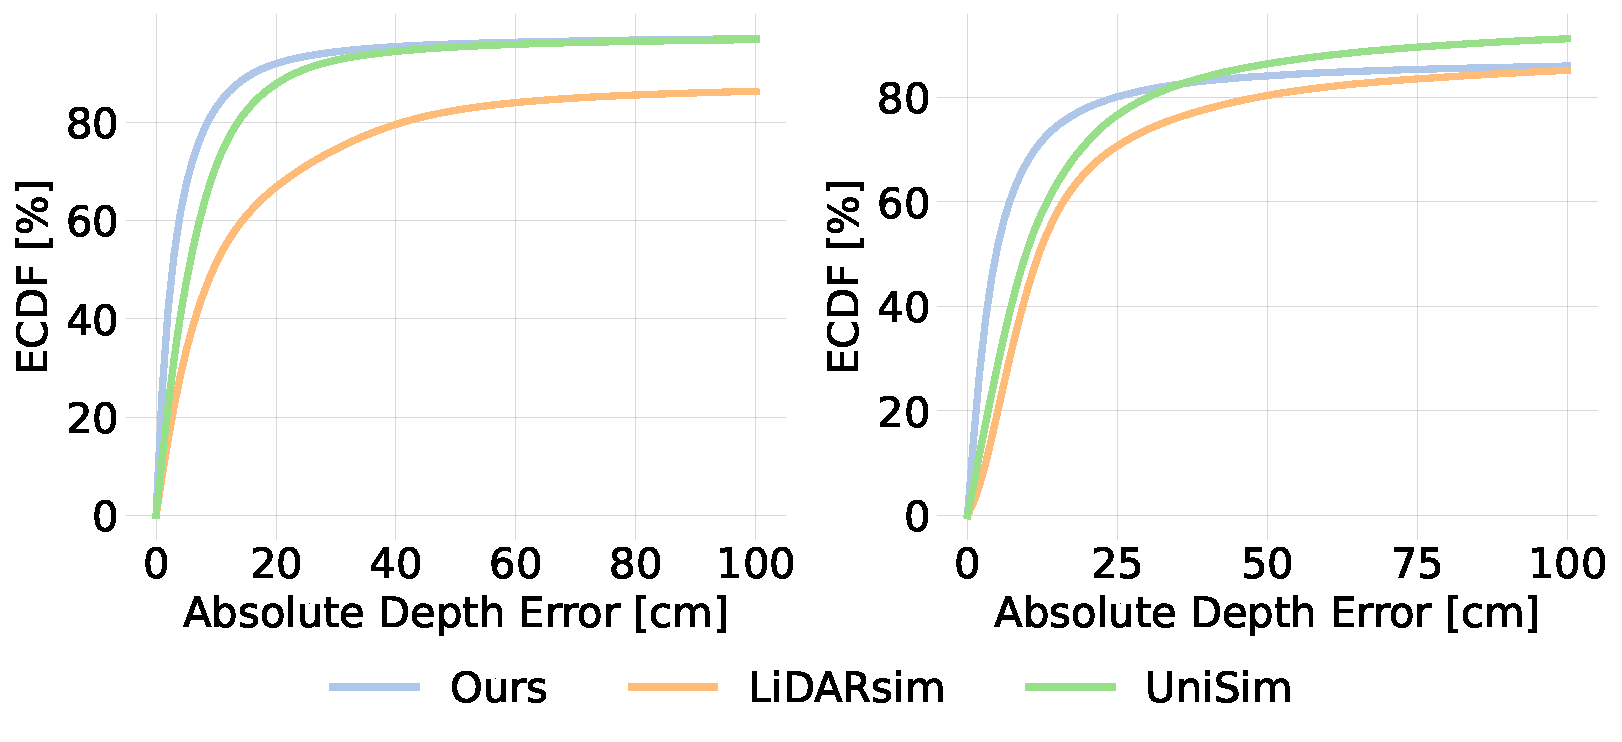
\includegraphics[width=1\columnwidth]{Figures/ecdf_3_methods.pdf}
   
        \caption{ECDF plots showcasing range errors across all the points (left) and specifically for points associated with dynamic vehicles (right). Our neural fields composition demonstrates superior performance over LiDARsim~\cite{manivasagam2020lidarsim} and UniSim~\cite{yang2023unisim}, especially in the context of dynamic vehicles.}
   \label{fig:ecdf}
   
\end{figure}
\begin{figure}[t]
    \centering
        \includegraphics[width=1\columnwidth]{Figures/errormap_static.pdf}
        
        \caption{Qualitative results of range estimation. Regions with gross errors (-100 \bwrDyNFL~100 cm) are highlighted.
        }
    \label{fig:error_map}
\end{figure}
\subsection{LiDAR Novel View Synthesis Evaluation} \label{sec:lidar_eval}
\paragraph{LiDAR NVS in dynamic scenes}
Quantitative comparisons with baseline methods are detailed in~\cref{tab:waymodynamic}. \dynfl notably outperforms LiDARsim~\cite{manivasagam2020lidarsim} and UniSim~\cite{yang2023unisim} in range reconstruction. This improvement is largely due to our SDF-based neural scene representation, which incorporates the physical aspects of LiDAR sensing. Additionally, our method employs a ray drop test when rendering multiple neural fields, leading to a more accurate reconstruction of dynamic vehicles, as evidenced in~\cref{fig:errormap_dynamic} and further supported by the data in~\cref{fig:ecdf}.


\begin{figure*}[t]
    \centering
        \includegraphics[width=1.0\textwidth]
        {Figures/sensor_manipulation.pdf}
        
        \caption{LiDAR novel view synthesis by changing sensor elevation angle~($\theta$), poses~($x,y,z$) and number of beams on \textit{Waymo Dynamic} dataset. The points are color-coded by the intensity values (0 \bwrDyNFL~0.25).}
    \label{fig:lidar_nvs}
\end{figure*}
\paragraph{LiDAR NVS in static scenes}
In addition to dynamic scenes, we evaluate \dynfl against baseline methods in static scenarios, with the results detailed in~\cref{tab:waymostatic} and~\cref{fig:error_map}. \dynfl excels in reconstructing geometry in most cases. A key observation is its superior performance in reconstructing planar regions (\eg the ground shown in~\cref{fig:error_map}), especially when compared to NFL~\cite{Huang2023nfl}, which also uses a neural field for surface representation. This improvement is largely due to the enhanced surface regularizations provided by our advanced SDF-based surface modeling approach.


\begin{table}[t]
    \setlength{\tabcolsep}{4pt}
    \renewcommand{\arraystretch}{1.2}
	\centering
	\resizebox{0.5\columnwidth}{!}{
    \small
    \begin{tabular}{l|ccc}
    \toprule
    Datasets  & MAE $\downarrow$ &  MedAE $\downarrow$ & CD $\downarrow$ \\
    \midrule
    TownClean~ & 26.7(\textcolor{green}{-1.5}) & 0.7(\textcolor{green}{-0.2}) & 6.7(\textcolor{green}{-0.5})\\
    Waymo Interp~ & 28.3 (\textcolor{red}{0.1}) & 4.7 (\textcolor{green}{-0.2}) & 12.5 (\textcolor{green}{-0.1})\\
    Waymo Dynamic~ & 30.8 (\textcolor{green}{-0.3}) & 3.0 (\textcolor{green}{-0.2}) & 10.9 (\textcolor{green}{-0.3})\\
    \bottomrule
    \end{tabular}
    }
    
	\caption{Ablation study of volume rendering for active sensing.}
	\label{tab:active_sensing}
\end{table}
\begin{table}[t]
    \setlength{\tabcolsep}{4pt}
    \renewcommand{\arraystretch}{1.2}
	\centering
	\resizebox{0.5\columnwidth}{!}{
    \small
    \begin{tabular}{l|ccc}
    \toprule
    Datasets  & MAE $\downarrow$ &  MedAE $\downarrow$ & CD $\downarrow$ \\
    \midrule
    TownReal~ & 33.9(\textcolor{green}{-3.3}) & 2.1(\textcolor{green}{-0.0}) & 10.4(\textcolor{green}{-1.2})\\
    Waymo Interp~ & 28.3 (\textcolor{green}{-0.3}) & 4.7 (\textcolor{green}{-0.1}) & 12.5 (\textcolor{green}{-0.3})\\
    \bottomrule
    \end{tabular}
    }
    
	\caption{Ablation study of the surface points' SDF regularisation.}
	\label{tab:surface_sdf}
\end{table}
\begin{figure}[t]
  \centering
   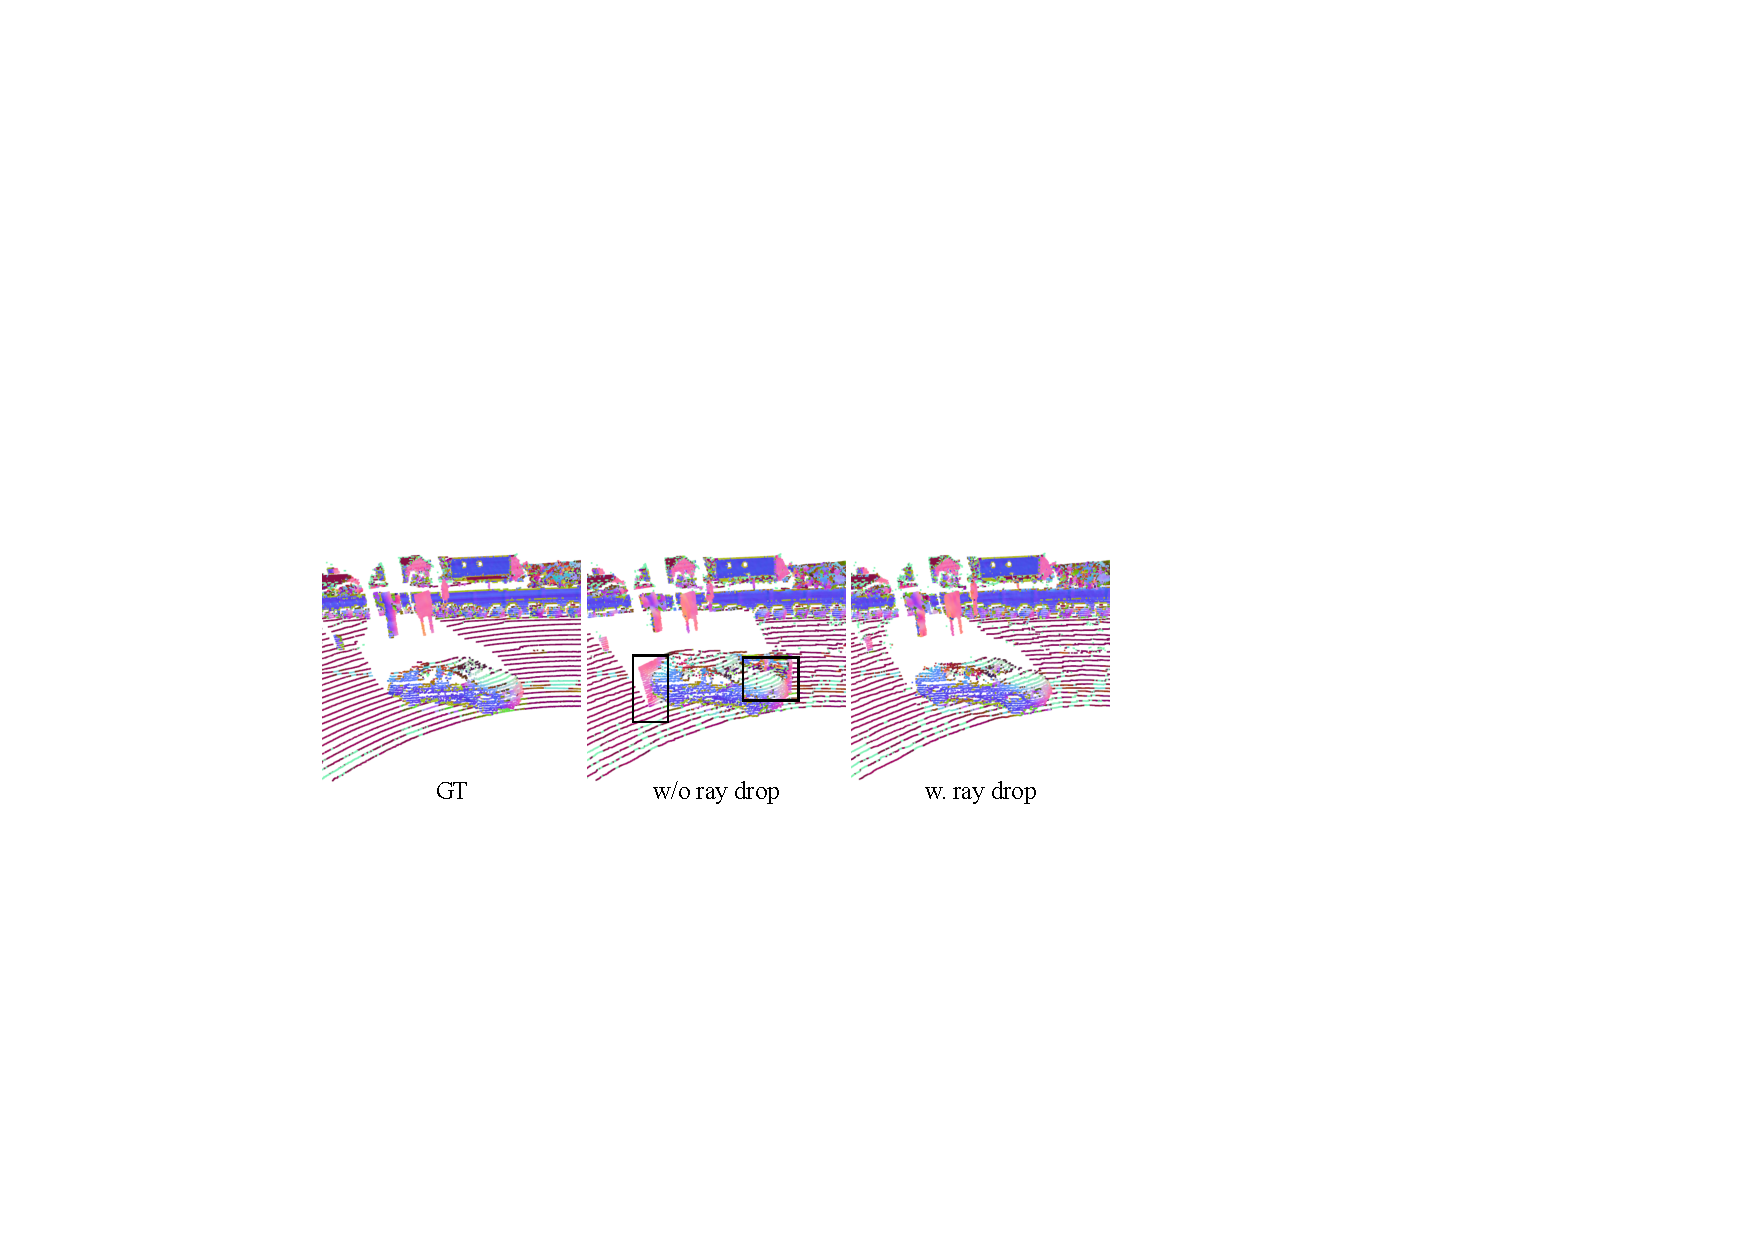
\includegraphics[width=1\linewidth]{Figures/intersectiontest.pdf}
   
   \caption{
   Qualitative results on \textit{Waymo Dynamic} dataset. Our model equipped with a ray drop module effectively composites multiple neural fields, re-simulating LiDAR scans of high quality.
   }
   % \caption{These figures exemplify the effectiveness of our field composition method leveraging ray drop probability from dynamic neural field. When all intersected rays are rendered for the dynamic neural field, noticeable artifacts appear due to disturbances from irrelevant fields (middle figure). The figures on the right showcase the complete composition method.
   % }
   % \caption{
   % }
    
   \label{fig:ablation_raydrop}
\end{figure}

\begin{figure}[t]
    \centering
        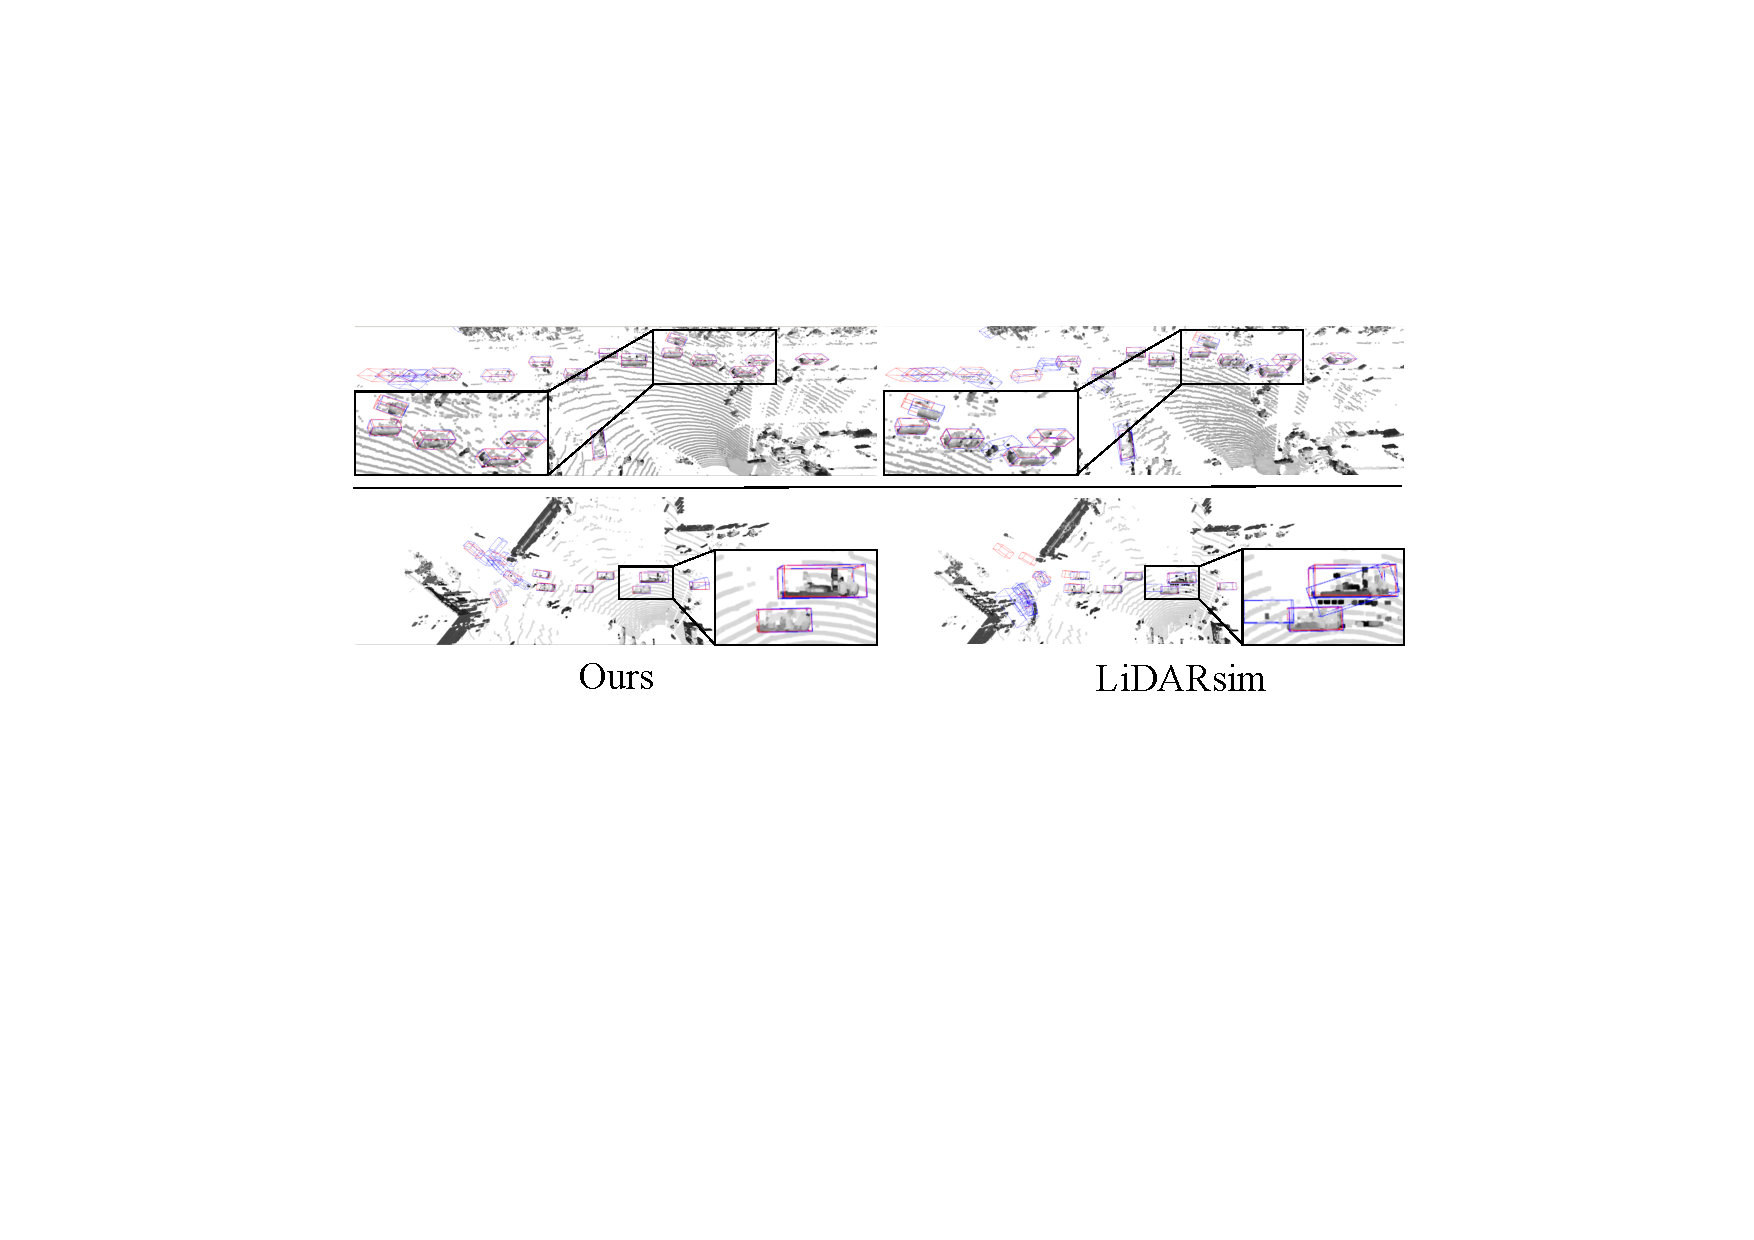
\includegraphics[width=0.8\columnwidth]{Figures/detection_result.pdf}
        \caption{Object detection results on \textit{Waymo Dynamic} dataset. The ground truth and predicted bounding boxes are marked in \textcolor{red}{red} and \textcolor{blue}{blue}, respectively.}
    \label{fig:detection}
    
\end{figure}
% \begin{table}[t]
% 	\centering
% 	\resizebox{0.8\columnwidth}{!}{
% 		\begin{tabular}{@{}lcccccccc@{}}
% 			\toprule
%              & \multicolumn{1}{c}{GT} & \multicolumn{3}{c}{Ours} & \multicolumn{3}{c}{LiDARSim\cite{manivasagam2020lidarsim}} \\
% 			  \cmidrule(r){2-2}\cmidrule(r){3-5} \cmidrule(l){6-8}
% 			Threshold & AP$\uparrow$ & \multicolumn{1}{c}{AP$\uparrow$}& \multicolumn{1}{c}{Agg.$\uparrow$}& \multicolumn{1}{c}{Dyn. Agg.$\uparrow$} & \multicolumn{1}{c}{AP$\uparrow$} & \multicolumn{1}{c}{Agg.$\uparrow$}& \multicolumn{1}{c}{Dyn. Agg.$\uparrow$} \\
% 			\midrule
% 			IoU$>$0.7 &0.85  &0.86 & \textbf{0.77}& \textbf{0.71}& \textbf{0.90} & 0.76 & 0.68\\
% 			IoU$>$0.5 &\textbf{0.98}  & 0.96 & \textbf{0.87}& \textbf{0.76}& 0.95 & 0.86& \textbf{0.76} \\
% 			\bottomrule
% 		\end{tabular}
% 	}
% 	\caption{Object detection results on \textit{Waymo Dyanmic} datasets.}
    
% 	\label{tab:detection}
% \end{table}

\begin{table}[t]
	\centering
		\begin{tabularx}{\columnwidth}{l|YYYYYYY}
			\toprule
             & \multicolumn{1}{c}{GT} & \multicolumn{3}{c}{Ours} & \multicolumn{3}{c}{LiDARSim\cite{manivasagam2020lidarsim}} \\
			  \cmidrule(r){2-2}\cmidrule(r){3-5} \cmidrule(l){6-8}
			Threshold & AP$\uparrow$ & \multicolumn{1}{c}{AP$\uparrow$}& \multicolumn{1}{c}{Agg.$\uparrow$}& \multicolumn{1}{c}{Dyn. Agg.$\uparrow$} & \multicolumn{1}{c}{AP$\uparrow$} & \multicolumn{1}{c}{Agg.$\uparrow$}& \multicolumn{1}{c}{Dyn. Agg.$\uparrow$} \\
			\midrule
			IoU$>$0.7 &0.85  &0.86 & \textbf{0.77}& \textbf{0.71}& \textbf{0.90} & 0.76 & 0.68\\
			IoU$>$0.5 &\textbf{0.98}  & 0.96 & \textbf{0.87}& \textbf{0.76}& 0.95 & 0.86& \textbf{0.76} \\
			\bottomrule
		\end{tabularx}
	\caption{Object detection results on \textit{Waymo Dyanmic} datasets.}
    
	\label{tab:detection}
\end{table}
% \begin{table}[t]
% \setlength{\tabcolsep}{4pt}
% \renewcommand{\arraystretch}{1.2}
% \centering
% \resizebox{0.8\columnwidth}{!}{
% \begin{tabular}{l|ccc|ccc}
% \toprule
% & \multicolumn{3}{c|}{Vehicle} & \multicolumn{3}{c}{Background} \\
% Method & Recall $\uparrow$ & Precision $\uparrow$ & IoU $\uparrow$ & Recall $\uparrow$ & Precision $\uparrow$ & IoU $\uparrow$ \\
% \midrule
% i-NGP~\cite{muller2022instant} & \underline{93.2} & 85.9 & 80.9 & 98.3 & \underline{99.2} & 97.6\\
% DS-NeRF~\cite{deng2021depth} & 90.7 & \underline{87.1} & 80.2 & \underline{98.5} & 98.9 & 97.4\\
% URF~\cite{rematas2021urban} & 87.8 & 81.7 & 73.7 & 98.0 & 98.4 & 96.5\\
% Lidarsim~\cite{manivasagam2020lidarsim} & 90.5 & 70.5 & 65.9 & 94.9 & 99.0 & 94.0\\
% NFL density~\cite{Huang2023nfl}& \textbf{95.9} & 87.0 & \textbf{83.9} & 98.3 & \textbf{99.5} & \textbf{97.8}\\
% Ours & 90.5 & \textbf{89.2} & \underline{82.3} & \textbf{98.8} & 98.9 & \underline{97.7}\\
% \bottomrule
% \end{tabular}
% }
% 
% \caption{Semantic segmentation results on \textit{Waymo NVS} dataset.}
% \label{tab:sem_seg_nvs}
% \end{table}



\begin{table}[t]
\setlength{\tabcolsep}{4pt}
\renewcommand{\arraystretch}{1.2}
\centering
\resizebox{0.99\columnwidth}{!}{
\begin{tabular}{l|ccc|ccc}
\toprule
& \multicolumn{3}{c|}{Vehicle} & \multicolumn{3}{c}{Background} \\
Method & Recall $\uparrow$ & Precision $\uparrow$ & IoU $\uparrow$ & Recall $\uparrow$ & Precision $\uparrow$ & IoU $\uparrow$ \\
\midrule
i-NGP~\cite{mueller2022instant} & 91.8 & 83.6 & 78.1 & 97.9 & 99.2 & 97.1\\
DS-NeRF~\cite{kangle2021dsnerf} & 89.3 & 84.8 & 77.3 & 98.1 & 98.8 & 97.0\\
URF~\cite{rematas2021urban} & 86.9 & 79.8 & 72.0 & 97.7 & 98.5 & 96.2\\
Lidarsim~\cite{manivasagam2020lidarsim} & 89.6 & 68.9 & 64.0 & 94.5 & 98.9 & 93.5\\
NFL~\cite{Huang2023nfl}& \textbf{94.5} & 84.8 & 80.9 & 97.8 & \textbf{99.4} & \textbf{97.3}\\
Ours & 90.5 & \textbf{88.4} & \textbf{81.1} & \textbf{98.5} & 98.7 & \textbf{97.3}\\
\bottomrule
\end{tabular}
}

\caption{Semantic segmentation results on \textit{Waymo NVS} dataset.}
\label{tab:sem_seg_nvs_ours}

\end{table}




\subsection{Ablation Study}
\paragraph{SDF-based volume rendering for active sensing}
We begin by assessing the efficacy of our SDF-based volume rendering for active sensor, the results are shown in~\cref{tab:active_sensing}. When compared to our baseline that uses the SDF-based volume rendering for passive sensing, \dynfl demonstrates enhanced performance in both synthetic (\textit{TownClean}) and real-world (\textit{Waymo Interp} and \textit{Waymo Dynamic}) datasets, indicating the importance of incorporating the physical sensing process of LiDAR in addressing the inverse problem.


\paragraph{Neural fields composition} 
To validate the efficacy of our two-stage neural field composition approach, we compare it with an alternative approach utilized in UniSim~\cite{yang2023unisim}. The results are shown in~\cref{tab:waymodynamic}. UniSim~\cite{yang2023unisim} blends different neural fields by sampling points from all intersected neural fields, followed by a single evaluation of volume rendering to produce the final LiDAR scan. In contrast, our method independently renders from each intersecting neural field first, and then combines these measurements into a final measurement using a ray drop test (\cf~\cref{fig:ablation_raydrop}). This approach leads to a notable improvement in geometry reconstruction over UniSim~\cite{yang2023unisim}, exemplified by our method halving the Median Absolute Error (MedAE) across all points. This enhancement is even more evident when focusing solely on points related to dynamic vehicles (\cf~\cref{fig:ecdf}).
% 

\paragraph{Surface points' SDF constraint}
We examine the importance of the surface points' SDF constraint discussed in ~\cref{sec:optmisation} on \textit{Town Real} and \textit{Waymo Interp} datasets. The results shown in \cref{tab:surface_sdf} suggest that our method yields improved geometry reconstruction quality by additionally enforcing LiDAR points to have zero SDF values. 


\subsection{Auxiliary Task Evaluations} 
\label{sec:downstream}
To assess the fidelity of our neural re-simulation and gauge the domain gap between re-simulated and real scans, we evaluate their applicability in two downstream tasks: object detection and semantic segmentation.


\paragraph{Object detection}
We utilize the pre-trained FSDv2~\cite{fan2023fsdv2} model for object detection and conduct evaluations on the re-simulated LiDAR scans within the \textit{Waymo Dynamic} dataset. Our results are compared against those from LiDARsim~\cite{manivasagam2020lidarsim}, with the findings detailed in~\cref{tab:detection} and~\cref{fig:detection}. Notably, \dynfl exhibits a more substantial detection agreement with the predictions on real LiDAR scans. This indicates a higher fidelity in our re-simulations and a reduced domain gap relative to actual scans.


\paragraph{Semantic segmentation}
For semantic segmentation, we use the pre-trained SPVNAS model~\cite{tang2020searching}, with the results presented in~\cref{tab:sem_seg_nvs_ours}. \dynfl improves over baseline methods according to most evaluation metrics, underscoring the realism of our re-simulated LiDAR scans.



\subsection{Scene Editing}
Beyond LiDAR novel view synthesis by adjusting the sensor configurations (\cf \cref{fig:lidar_nvs}), we additionally demonstrate the practicality of our compositional neural fields approach through two scene editing applications.

\begin{figure}[t]
    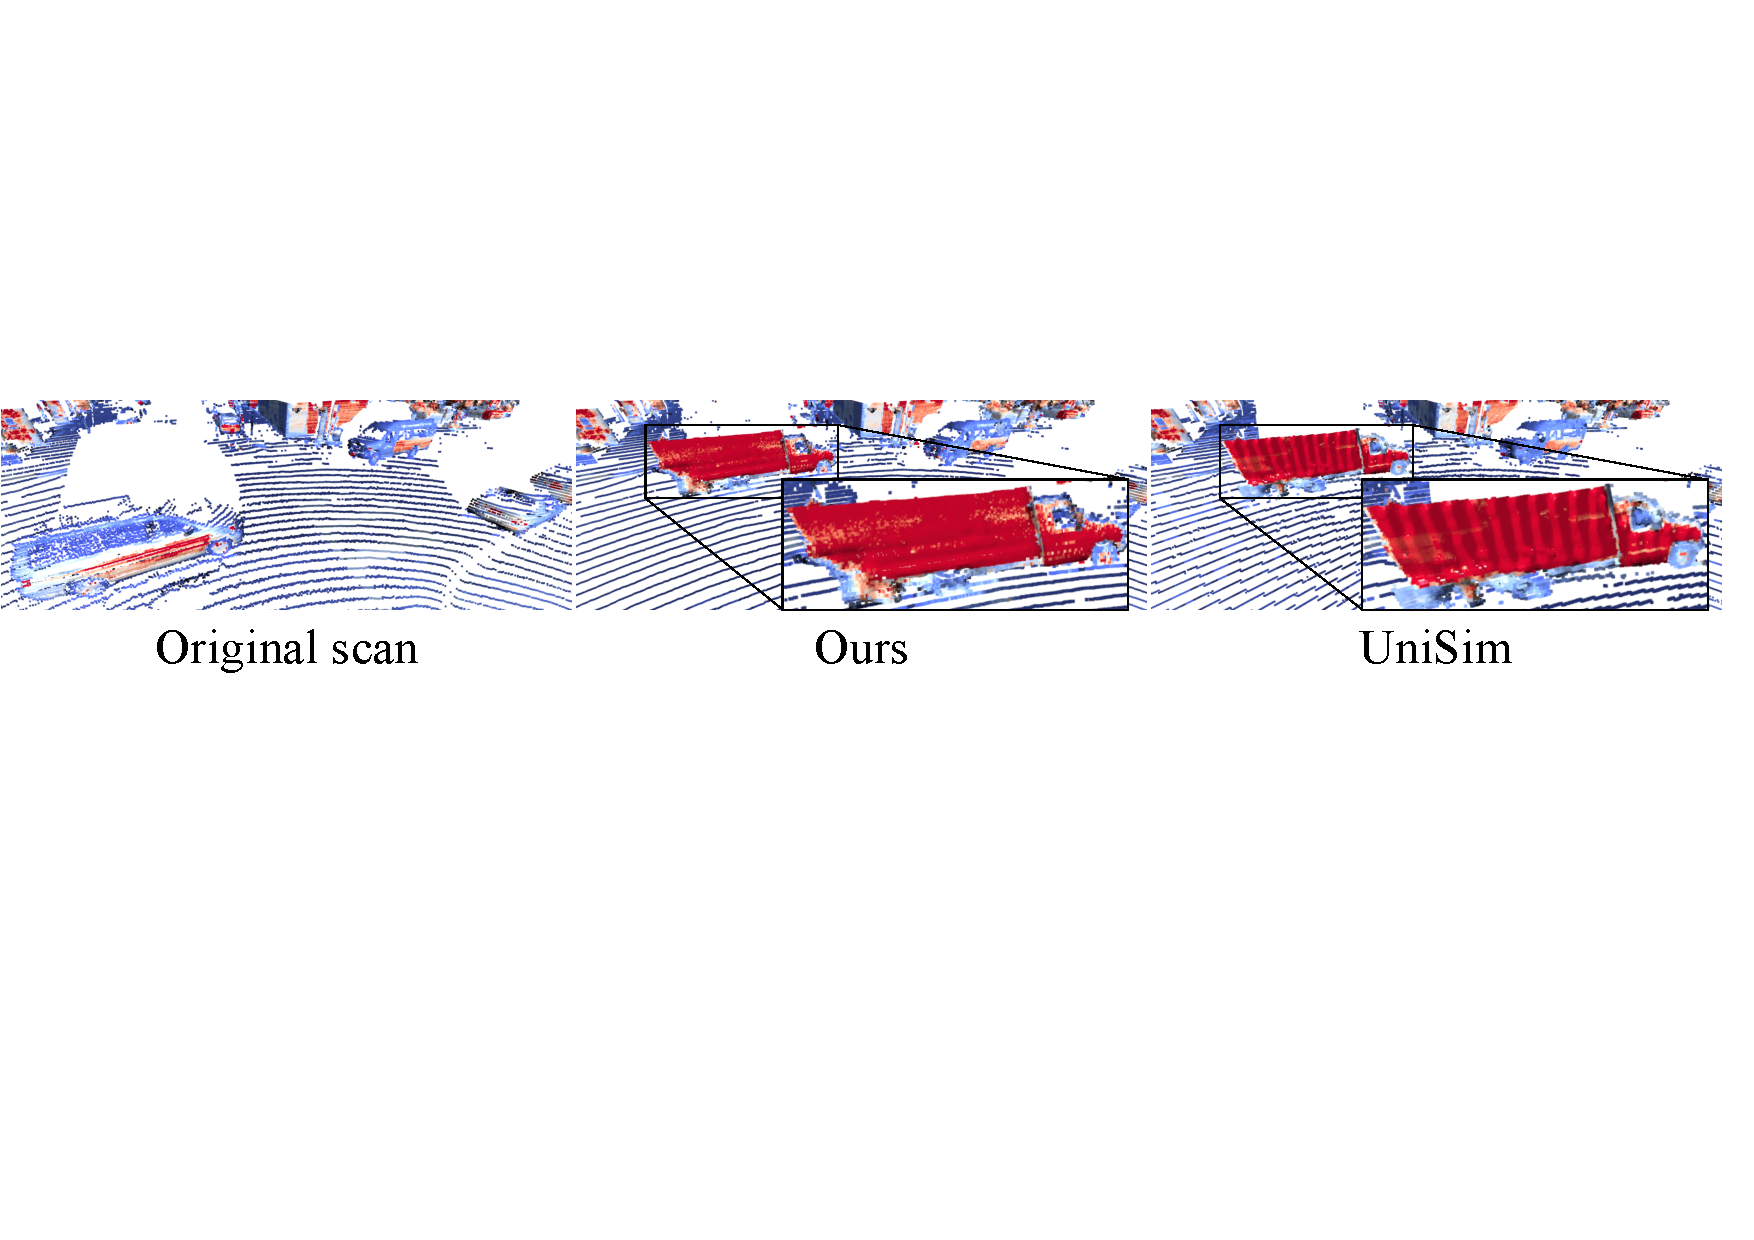
\includegraphics[width=1.0\linewidth]{Figures/vehicle_insertion.pdf}
    
    \caption{
    Qualitative results of object removal and insertion. \dynfl seamlessly inserts the neural asset (truck) into a new scene attributed to our superior compositional rendering scheme. In contrast, UniSim~\cite{yang2023unisim} struggles to accurately model geometry.
    }
    \label{fig:vehicle_insertion}
\end{figure}
\paragraph{Insert object from one scene into another}
Our explicit neural scene de-composition and flexible composition technique enable seamless insertion and removal of neural assets across scenes. As demonstrated in~\cref{fig:vehicle_insertion}, we are able to replace a car from one scene with a truck from another scene, achieving accurate reconstruction of both geometry and intensity. In contrast, UniSim~\cite{yang2023unisim} struggles to preserve high quality geometry. This highlights the significant potential of our approach in generating diverse and realistic LiDAR scans for autonomous driving scenarios.

\begin{figure}[t]
    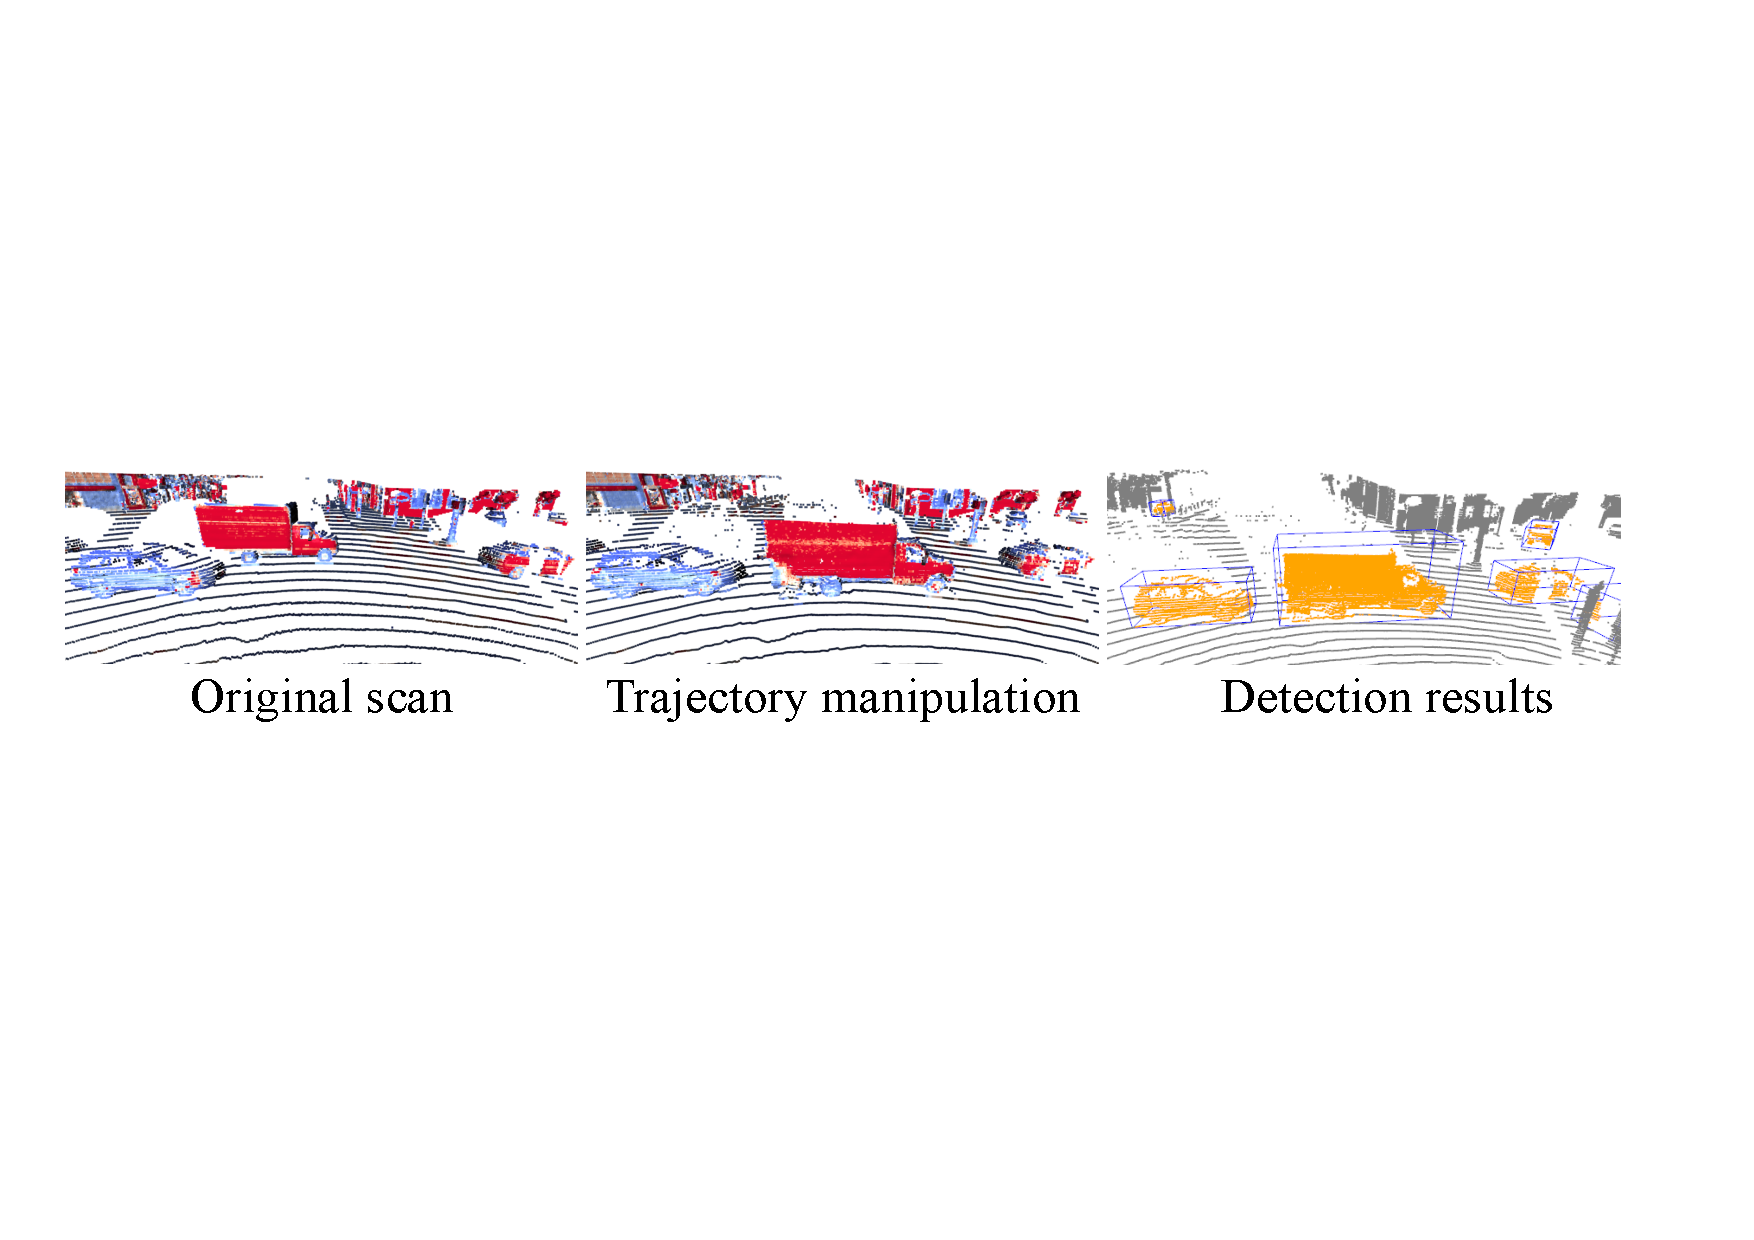
\includegraphics[width=1.0\columnwidth]{Figures/trajectory_manipulation.pdf}
    
    \caption{Qualitative results of object trajectory manipulation. The truck can be successfully detected after manipulation, indicating high-realism LiDAR re-simulation achieved by \dynfl.}
    \label{fig:traj}
    
\end{figure}
\paragraph{Manipulate the trajectory of dynamic objects}
\dynfl also facilitates the manipulation of moving objects' trajectories by simply adjusting their relative poses to the canonical bounding box. Representative results are shown in ~\cref{fig:traj}. The high realism of our re-simulation is also indicated by the successful detection of inserted virtual objects.

\section{Limitations and Future Work}
We present DyNFL, a compositional neural fields approach for LiDAR re-simulation. Our method excels previous art in both static and dynamic scenes, offering powerful scene editing capabilities that open up opportunities for generating diverse and high-quality scenes, to evaluate an autonomy system trained only on real data in closed-loop.

Despite achieving the state-of-the-art performance, there are still limitations we aim to address in future work. Firstly, \dynfl faces challenges in view synthesis of dynamic vehicles from unseen angles. This difficulty arises from the complexity of creating an a-priori model that can accurately complete unseen regions and simulate point cloud noise, ray drops patterns etc. Secondly, our method currently relies on object detection and tracking annotations, and its performance may be compromised when given inaccurate labels. Overcoming this dependency, exploring 4D representations while retaining scene editing flexibility, stands out as a crucial challenge for future research.


\paragraph{Acknowledgements.}
{Or Litany is a Taub fellow and is supported by the Azrieli Foundation Early Career Faculty Fellowship.}

\clearpage
\section{Appendix}
In this supplementary material, we first provide additional information about the datasets for our evaluations and implementation details of our proposed method in~\cref{sec:sup_dataset}. Next, we present more qualitative results in~\cref{sec:sup_visual}. Please also check the supplemental video for more results showcasing our performance. Finally, we provide the complete derivations of the SDF-based volume rendering for active sensor in~\cref{sec:sup_sdf_vol_render}. 

\section{Datasets and implementation details}\label{sec:sup_dataset}
\subsection{Datasets}
\paragraph{\textit{Waymo Dynamic}} For the \textit{Waymo Dynamic} dataset, we take them from 4 scenes of \textit{Waymo Open Dataset}~\cite{sun2020scalability}. There are multiple moving vehicles inside each scene. 50 consecutive frames are taken from each scene for our evaluation. The vehicles are deemed as \textit{dynamic} if the speed is $>1\,$m/s. in any of the 50 frames. The corresponding scene IDs on \textit{Waymo Open Dataset} for our selected scenes are shown as follows:
\begin{table}[!h]
    \setlength{\tabcolsep}{4pt}
    \renewcommand{\arraystretch}{1.2}
	\centering
	\resizebox{0.8\columnwidth}{!}{
    \begin{tabular}{l|c}
    \toprule
    & Scene ID \\
    \midrule
    Scene 1 & 1083056852838271990\_4080\_000\_4100\_000 \\
    Scene 2 & 13271285919570645382\_5320\_000\_5340\_000 \\
    Scene 3 & 10072140764565668044\_4060\_000\_4080\_000 \\
    Scene 4 & 10500357041547037089\_1474\_800\_1494\_800 \\
    \bottomrule
    \end{tabular}
    }
\end{table}

\subsection{Implementation details}
\paragraph{Ours} 
Our model is implemented based on nerfstudio\cite{nerfstudio}. For the static neural field, we sample $N_s=512$ points in total, with $N_u=256$ uniformly sampled points and $N_i=256$ weighted sampled points with 8 upsample steps. In each upsample step, 32 points are sampled based on the weight distribution of the previously sampled points. For each dynamic neural field, we sample $N_s=128$ points in total, with $N_u=64$ uniformly sampled points and $N_i=64$ weighted sampled points with 4 upsample steps. During training, we minimize the loss function using the Adam~\cite{kingma2014adam} optimiser, with an initial learning rate of 0.005. It linearly decays to 0.0005 towards the end of training. For the loss weights, we use $w_{\zeta}=3, w_{e}=50, w_{\text{drop}}=0.15, w_{s}=1$, and  $w_{\text{eik}}=0.3$. The batch size is 4096 and we train the model for 60000 iterations on a single RTX3090 GPU with float32 precision.

\paragraph{LiDARsim} We re-implement the LiDARsim~\cite{manivasagam2020lidarsim} as one of our baselines. 
First, we estimated point-wise normal vectors by considering all points within a 20 cm radius ball within the training set. Following this, we applied voxel down-sampling~\cite{tang2022torchsparse}, employing a 4 cm voxel size to reconstruct individual disk surfels at each point. The surfel orientation is defined based on the estimated normal vector. During inference, we apply the ray-surfel intersections test to determine the intersection points, thus the range and intensity values. We select a fixed surfel radius of 6 cm for the \textit{Waymo} dataset and 12 cm for the \textit{Town} dataset.
To handle dynamic vehicles, we follow LiDARsim~\cite{manivasagam2020lidarsim} by aggregating the LiDAR points for each vehicle from all the training frames and representing them in the \textit{canonical} frame of each vehicle. During inference, we transform all the aggregated vehicle points from their \textit{canonical} frames to the world frame and run ray-surfel intersection.

\paragraph{UniSim} 
We re-implement UniSim's~\cite{yang2023unisim} rendering process for LiDAR measurements by replacing our ray-drop test-based neural fields composition method with its joint rendering method. For every ray $\mathbf{r} (\mathbf{o},\mathbf{d})$, we begin by conducting an intersection test with all dynamic bounding boxes in the scene to identify the near and far limits. We then uniformly sample 512 points along each ray, assigning each point to either a dynamic neural field, if it falls within a dynamic bounding box, or to the static neural field otherwise. After sampling, we query the SDF and intensity values from the relevant neural fields. Finally, using the SDF-based volume rendering formula in Eq.~\ref{eq:depth_render} for active sensors, we calculate the weights and perform the rendering. Note that we use the same neural field architecture as in our method.
\begin{figure*}[t!]
  \centering
   \includegraphics[width=1\textwidth]{Figures_sup/4_scenes_sup.pdf}
   \caption{Visualization of 4 selected scenes from \textit{Waymo Dynamic} dataset. For each scene, we aggregate 50 frames. In the first row, points are color-coded by the intensity values(0 ~\bwrDyNFL~ 0.25). In the second row, dynamic vehicles are painted as \textcolor{yellow}{yellow}.}
   \label{fig:4_scenes_supp}
\end{figure*}

\begin{figure*}[t!]
  \centering
   \includegraphics[width=1\textwidth]{Figures_sup/supp_scene_edit.pdf}
   \caption{Visualization of scene editing capabilities. We showcase 3 kinds of scene editing capabilities including vehicle removal(left), trajectory manipulation(middle) and vehicle insertion(right). The first row represents the original scenes, the second row demonstrates the scenes after editing. All points are color-coded by the intensity values(0 ~\bwrDyNFL~ 0.25).}
   \label{fig:scene_editing_supp}
\end{figure*}

\section{More qualitative results}\label{sec:sup_visual}
In this section, we provide more qualitative results. In \cref{fig:4_scenes_supp}, we showcase the 4 scenes from \textit{Waymo dynamic} dataset. We show additional scene editing results in~\cref{fig:scene_editing_supp}. Please check the supplementary videos for more qualitative results.

\clearpage
\clearpage
\section{SDF-based volume rendering for active sensor}\label{sec:sup_sdf_vol_render}
In this section, we start by introducing the preliminary of NeRF~\cite{mildenhall2020nerf} following terminology as described in~\cite{tagliasacchi2022volume}. Then we provide the full derivation of the SDF-based volume rendering for active sensor. 

\subsection{Preliminary}\label{sec:supp_pre}
\paragraph{Density}
For a ray emitted from the origin $\origin \in \real^3$ towards direction $\dir \in \real^3$, the \textit{density} $\density_\zeta$ at range $\zeta$ indicates the likelihood of light interacting with particles at that point $\ray_\zeta = \origin + \zeta \dir$. This interaction can include absorption or scattering of light. In passive sensing, density $\density$ is a critical factor in determining how much light from the scene's illumination is likely to reach the sensor after passing through the medium.
\paragraph{Transmittance} quantifies the likelihood of light traveling through a given portion of the medium without being scattered or absorbed. Density is closely tied to the transmittance function $\transmittance(\zeta)$, which indicates the probability of a ray traveling over the interval $[0, \zeta)$ without hitting any particles. Then the probability $\transmittance(\zeta {+} d\zeta)$ of \emph{not} hitting a particle when taking a differential step $d\zeta$ is equal to $\transmittance(\zeta)$, the likelihood of the ray reaching $\zeta$, times $(1 - d\zeta \cdot \density(\zeta))$, the probability of not hitting anything during the step:
% 
\begin{align}
\transmittance(\zeta+d\zeta) =& \transmittance(\zeta) \cdot (1 - d\zeta \cdot \density(\zeta))
\\
\frac{\transmittance(\zeta+d\zeta) - \transmittance(\zeta)}{d\zeta} \equiv& \transmittance'(\zeta) = -\transmittance(\zeta) \cdot \sigma(\zeta) 
\label{eq:derivative}
\end{align}
% 
We solve the differential equation as follows:
%
\begin{align}
\transmittance'(\zeta) &= -\transmittance(\zeta) \cdot \density(\zeta) \\
\frac{\transmittance'(\zeta)}{\transmittance(\zeta)} &= -\density(\zeta) \\
\int_a^b \frac{\transmittance'(\zeta)}{\transmittance(\zeta)} \; d\zeta &= -\int_a^b \density(\zeta) \; d\zeta \\
\left. \log \transmittance(\zeta) \right|_a^b &= -\int_a^b \density(\zeta) \; d\zeta \\
\transmittance(a \rightarrow b) \equiv \frac{\transmittance(b)}{\transmittance(a)} &= \exponential{-\int_a^b \density(\zeta) \; d\zeta}   
\end{align}
% 
Hence, for a ray segment between $\zeta_0$ and $\zeta$, transmittance is given by:

\begin{equation}
\transmittance_{\zeta_0 \rightarrow \zeta} \equiv \frac{\transmittance_{\zeta}}{\transmittance_{\zeta_0}} = exp({-\int_{\zeta_0}^\zeta \density_t dt})\;,
\label{eq:trans_ab}
\end{equation}
which leads to following factorization of the transmittance:
\begin{equation}
\transmittance_{\zeta} = \transmittance_{0 \rightarrow \zeta_0} \cdot \transmittance_{\zeta_0 \rightarrow \zeta}\;.
\label{eq:factor}
\end{equation}

\paragraph{Opacity}Opacity is the complement of transmittance and represents the fraction of light that is either absorbed or scattered in the medium. In a homogeneous medium with constant density $\density$  the opacity for a segment $[\zeta_j, \zeta_{j+1}]$ of length $\Delta \zeta$ is given by $\opacity_{\zeta_j} = 1 - exp(-\density \cdot \Delta \zeta)$
\subsection{SDF-based volume rendering for active sensor}\label{sec:sdf_active}
NeuS\cite{wang2021neus} derives the opaque density based on the SDF which is:
\begin{equation}
\begin{split}
\density_{\zeta_i} =&  \max\left(\frac{-\frac{d\Phi_s}{d\zeta_i}(f(\zeta_i))}{\Phi_s(f(\zeta_i))},0\right)\\
                  =& \max\left(\frac{-(\nabla f(\zeta_i)\cdot \mathbf{v})\phi_s(f(\zeta_i))}{\Phi_s(f(\zeta_i))}, 0\right)
\end{split}
\label{eq:sigmoid_density}
\end{equation}
where $\Phi_s$ represents the Sigmoid function, $f$ is the SDF function that maps a range $\zeta$ to the SDF value of the point position $\origin + \dir * \zeta$. Note that the integral term is computed by
\begin{equation}
\int \frac{-(\nabla f(\zeta)\cdot \mathbf{v})\phi_s(f(\zeta))}{\Phi_s(f(\zeta))}d\zeta = -\ln(\Phi_s(f(\zeta))) + C,
\label{eq:intergration_density}
\end{equation}
% We can then calculate the accumulated transmittance from \ref{eq:trans_ab} using \ref{eq:intergration_density}:
% % 
% \begin{align}
% \transmittance_\zeta = \transmittance(0 \rightarrow \zeta) 
% % &= \prod_{k=1}^{n-1} \transmittance(t_k \rightarrow t_{k+1}) 
% &= \exponential{- \int_{0}^{\zeta} \density(t) \; dt} 
% = \Phi_s(f(\zeta))
% \label{eq:trans_const}
% \end{align}
We extend the density-based volume rendering for active sensor to SDF-based. Starting from the passive SDF-based volume rendering \cite{wang2021neus}, We substitute the density $\tilde{\density}$ with opaque density in \ref{eq:sigmoid_density}
and evaluate the radiant power integrated from ray segment [a,b] with constant reflectivity $\reflectivity_a$.

Consider the case where $-(\nabla f(\zeta)\cdot \mathbf{v})>0$ within the ray segment $[a,b]$, we have
\begin{align}
P(a \rightarrow b)
&= \int_a^b \transmittance^2(a\rightarrow t) \cdot \tilde{\density}_t \cdot \reflectivity(t)  \; dt
\\
&= \reflectivity_a \int_a^b \transmittance^2(a\rightarrow t) \cdot \tilde{\density}_t \; dt
\\
&= \reflectivity_a \int_a^b \exponential{-\int_a^t 2\tilde{\density}(u) \; du} \cdot \tilde{\density}_t \; dt
\\
&= \reflectivity_a \int_a^b \exponential{-2\int_a^t \tilde{\density}(u) \; du} \cdot \tilde{\density}_t \; dt
\\
&= \reflectivity_a \int_a^b \exponential{\left. 2\ln(\Phi_s(f(u)))\right|_a^t} \cdot \tilde{\density}_t \; dt
\\
% &= \reflectivity_a \int_a^b \exponential{2\ln(\Phi_s(f(t))) - 2\ln(\Phi_s(f(a)))} \cdot \tilde{\density}_t \; dt \\
&= \reflectivity_a \int_a^b \exponential{2\ln(\Omega_t) - 2\ln(\Omega_a)} \cdot \tilde{\density}_t \; dt 
\\
&= \reflectivity_a \int_a^b \frac{{\Omega_t}^2}{{\Omega_a}^2} \cdot \tilde{\density}_t \; dt ~~~~\text{\textbf{let} $\Omega_x = \Phi_s(f(x))$}
\\
&= \frac{\reflectivity_a}{{\Omega_a}^2} \int_a^b {\Omega_t}^2 \cdot \tilde{\density}_t \; dt 
\\
&= \frac{\reflectivity_a}{{\Omega_a}^2} \int_a^b -\frac{d\Phi_s}{dt}(f(t)) \cdot \Phi_s(f(t)) \; dt 
% \quad \text{$\tilde{\density}_t = \frac{-\frac{d\Phi_s}{d t}(f(t))}{\Phi_s(f(t))}$}
\\
&= \frac{\reflectivity_a}{{\Omega_a}^2} ( \left. -\frac{1}{2}{\Phi_s(f(t))}^2 \right|_a^b) \\
&= \frac{\reflectivity_a}{{\Omega_a}^2} (\frac{1}{2}{\Phi_s(f(a))}^2 -\frac{1}{2}{\Phi_s(f(b))}^2 )\\
&= \frac{{\Phi_s(f(a))}^2 -{\Phi_s(f(b))}^2}{{2\Phi_s(f(a))}^2} \cdot \reflectivity_a 
% \quad \text{$T_a$ = $\Phi_s(f(a))$}
\label{eq:homogeneous}
\end{align}
%\cref{eq:trans_const}

Consider the case where $-(\nabla f(\zeta)\cdot \mathbf{v})<0$ within the ray segment $[a,b]$, we have
\begin{align}
P(a \rightarrow b)
&= \int_a^b \transmittance^2(a\rightarrow t) \cdot \tilde{\density}_t \cdot \reflectivity(t)  \; dt
\\
&= \int_a^b \transmittance^2(a\rightarrow t) \cdot 0 \cdot \reflectivity(t)  \; dt
\\
&= 0
\end{align}
Hence we conclude 
\begin{align}
P(a \rightarrow b)
&= \max\left(\frac{{\Phi_s(f(a))}^2 -{\Phi_s(f(b))}^2}{{2\Phi_s(f(a))}^2},0\right) \cdot \reflectivity_a 
\end{align}

\paragraph{Volume rendering of piecewise constant data}
Combining the above, we can evaluate the volume rendering integral through a medium with piecewise constant reflectivity:
% 
\begin{align}
P(\zeta_{N+1}) &= \sum_{n=1}^N \int_{\zeta_n}^{\zeta_{n+1}} \transmittance^2(\zeta) \cdot \tilde{\density}_{\zeta} \cdot \reflectivity_{\zeta_n} \; d\zeta
\\
&= \sum_{n=1}^N \int_{\zeta_n}^{\zeta_{n+1}} \transmittance^2_{\zeta_n} \cdot \transmittance^2(\zeta_n \shortto \zeta) \cdot \tilde{\density}_{\zeta} \cdot \reflectivity_{\zeta_n} \; d\zeta 
% &&\text{from \ref{eq:factor}}
\\
&= \sum_{n=1}^N \transmittance^2_{\zeta_n}  \int_{\zeta_n}^{\zeta_{n+1}} \transmittance^2(\zeta_n \rightarrow \zeta) \cdot \tilde{\density}_{\zeta} \cdot \reflectivity_{\zeta_n} \; d\zeta \\
% &&\text{constant}
% \\
&=\sum_{n=1}^N \transmittance^2_{\zeta_n} P(\zeta_n \rightarrow \zeta_{n+1})
\\
&= \sum_{n=1}^N \transmittance^2_{\zeta_n} \cdot \tilde{\weight}_{\zeta_n} \cdot \reflectivity_{\zeta_n},
% &&\text{from \ref{eq:homogeneous}}
\end{align}

where 
\begin{align}
\tilde{\weight}_{\zeta_n} \equiv \max\left(\frac{{\Phi_s(f(\zeta_n)}^2 -{\Phi_s(f(\zeta_{n+1}))}^2}{{2\Phi_s(f(\zeta_n))}^2},0\right)
\end{align}
% 
% This leads to the volume rendering equations from NeRF~\cite[Eq.3]{mildenhall2020nerf}:
% % 
% \begin{align}
% P(\zeta_{N+1}) = \sum_{n=1}^N \transmittance^2_{\zeta_n} \cdot \frac{{\Phi_s(f(\zeta_n))}^2 -{\Phi_s(f(\zeta_{n+1}))}^2}{{2\Phi_s(f(\zeta_n))}^2} \cdot \reflectivity_{\zeta_n}
% \label{eq:final_radiant}
% \end{align}
% % 
% Since the opacity is always greater than 0, we can express the opacity as
% \begin{equation}
%     \tilde{\weight}_{\zeta_n} \equiv max(\frac{{\Phi_s(f(\zeta_n))}^2 -{\Phi_s(f(\zeta_{n+1}))}^2}{{2\Phi_s(f(\zeta_n))}^2}, 0)
%     \label{eq:opacity}
% \end{equation}

The discrete accumulated transmittance $\transmittance$ can be calculated as follows:

Consider the case where $-(\nabla f(\zeta)\cdot \mathbf{v}) > 0$ in $[\zeta_n, \zeta_{n+1}]$: 
%
\begin{align}
\transmittance_{\zeta_n} 
&=\prod_{i=1}^{n-1}(\exp(-\int_{\zeta_n}^{\zeta_{n+1}}\tilde{\density}_\zeta \; d\zeta) \\
&= \prod_{i=1}^{n-1}(\frac{\Phi_s(f(\zeta_{n+1}))}{\Phi_s(f(\zeta_n))})\\
\transmittance^2_{\zeta_n}
&= \prod_{i=1}^{n-1}(\frac{{\Phi_s(f(\zeta_{n+1}))}^2}{{\Phi_s(f(\zeta_n))}^2})\\
&= \prod_{i=1}^{n-1}(1-2\tilde{\weight}_{\zeta_n})
\label{eq:dicrete_transmittance}
\end{align}

Consider the case where $-(\nabla f(\zeta)\cdot \mathbf{v}) < 0$ in $[\zeta_n, \zeta_{n+1}]$: 
\begin{align}
\transmittance_{\zeta_n} 
&=\prod_{i=1}^{n-1}(\exp(-\int_{\zeta_n}^{\zeta_{n+1}}\tilde{\density}_\zeta \; d\zeta) = \prod_{i=1}^{n-1}(1)
\\
\transmittance^2_{\zeta_n} &= \prod_{i=1}^{n-1}(1^2) = \prod_{i=1}^{n-1}(1-2\tilde{\weight}_{\zeta_n})
\end{align}
In conclusion, the radiant power can be reformulated as:

\begin{align}
P(\zeta_{N+1}) = \sum_{n=1}^N \transmittance^2_{\zeta_n} \cdot \tilde{\weight}_{\zeta_n} \cdot \reflectivity_{\zeta_n}
\label{eq:final_radiant2}
\end{align}
where $\transmittance^2_{\zeta_n} = \prod_{i=1}^{n-1}(1-2\tilde{\weight}_{\zeta_i})$


\paragraph{Depth volume rendering of piecewise constant data}

Note that $\tilde{\weight}_{\zeta_n} \in [0, 0.5], \transmittance^2_{\zeta_n} \in [0,1], \sum_{n=1}^N \transmittance^2_{\zeta_n} \cdot \tilde{\weight}_{\zeta_n} = 0.5$, for depth volumetric rendering, we have 
\begin{align}
    \zeta = \sum_{n=1}^N 2 \cdot \transmittance^2_{\zeta_n} \cdot \tilde{\weight}_{\zeta_n} \cdot \zeta_n
    =\sum_{n=1}^N w_n \cdot \zeta_n
    \label{eq:depth_render}
\end{align}
where $w_n = 2\tilde{\weight}_{\zeta_n} \cdot \prod_{i=1}^{n-1}(1-2\tilde{\weight}_{\zeta_i})$

\renewcommand{\subdir}{tex/ICCV2023_NFL}
\chapter[Dynamic LiDAR Re-simulation using Compositional Neural Fields]{Dynamic LiDAR Re-simulation using Compositional Neural Fields}
\label{chap:cvpr24}

Hanfeng Wu, Xingxing Zuo, Stefan Leutenegger, Or Litany, Konrad Schindler, Shengyu Huang \\
\textbf{IEEE/CVF Conference on Computer Vision and Pattern Recognition, 2024}\\
\\
(Author version; for typeset version please refer to the original conference paper.)\\

\providecommand{\subdir}{.}
\graphicspath{{\subdir/}}

\section*{Abstract}
We present Neural Fields for LiDAR (NFL), a method to optimise a neural field scene representation from LiDAR measurements, with the goal of synthesizing realistic LiDAR scans from novel viewpoints. 
NFL combines the rendering power of neural fields with a detailed, physically motivated model of the LiDAR sensing process, thus enabling it to accurately reproduce key sensor behaviors like beam divergence, secondary returns, and ray dropping.
We evaluate NFL on synthetic and real LiDAR scans and show that it outperforms explicit reconstruct-then-simulate methods as well as other NeRF-style methods on LiDAR novel view synthesis task. Moreover, we show that the improved realism of the synthesized views narrows the domain gap to real scans and translates to better registration and semantic segmentation performance. Project page: \url{https://research.nvidia.com/labs/toronto-ai/nfl}.
\newpage
\section{Introduction}
\begin{figure*}[t]
    \centering
        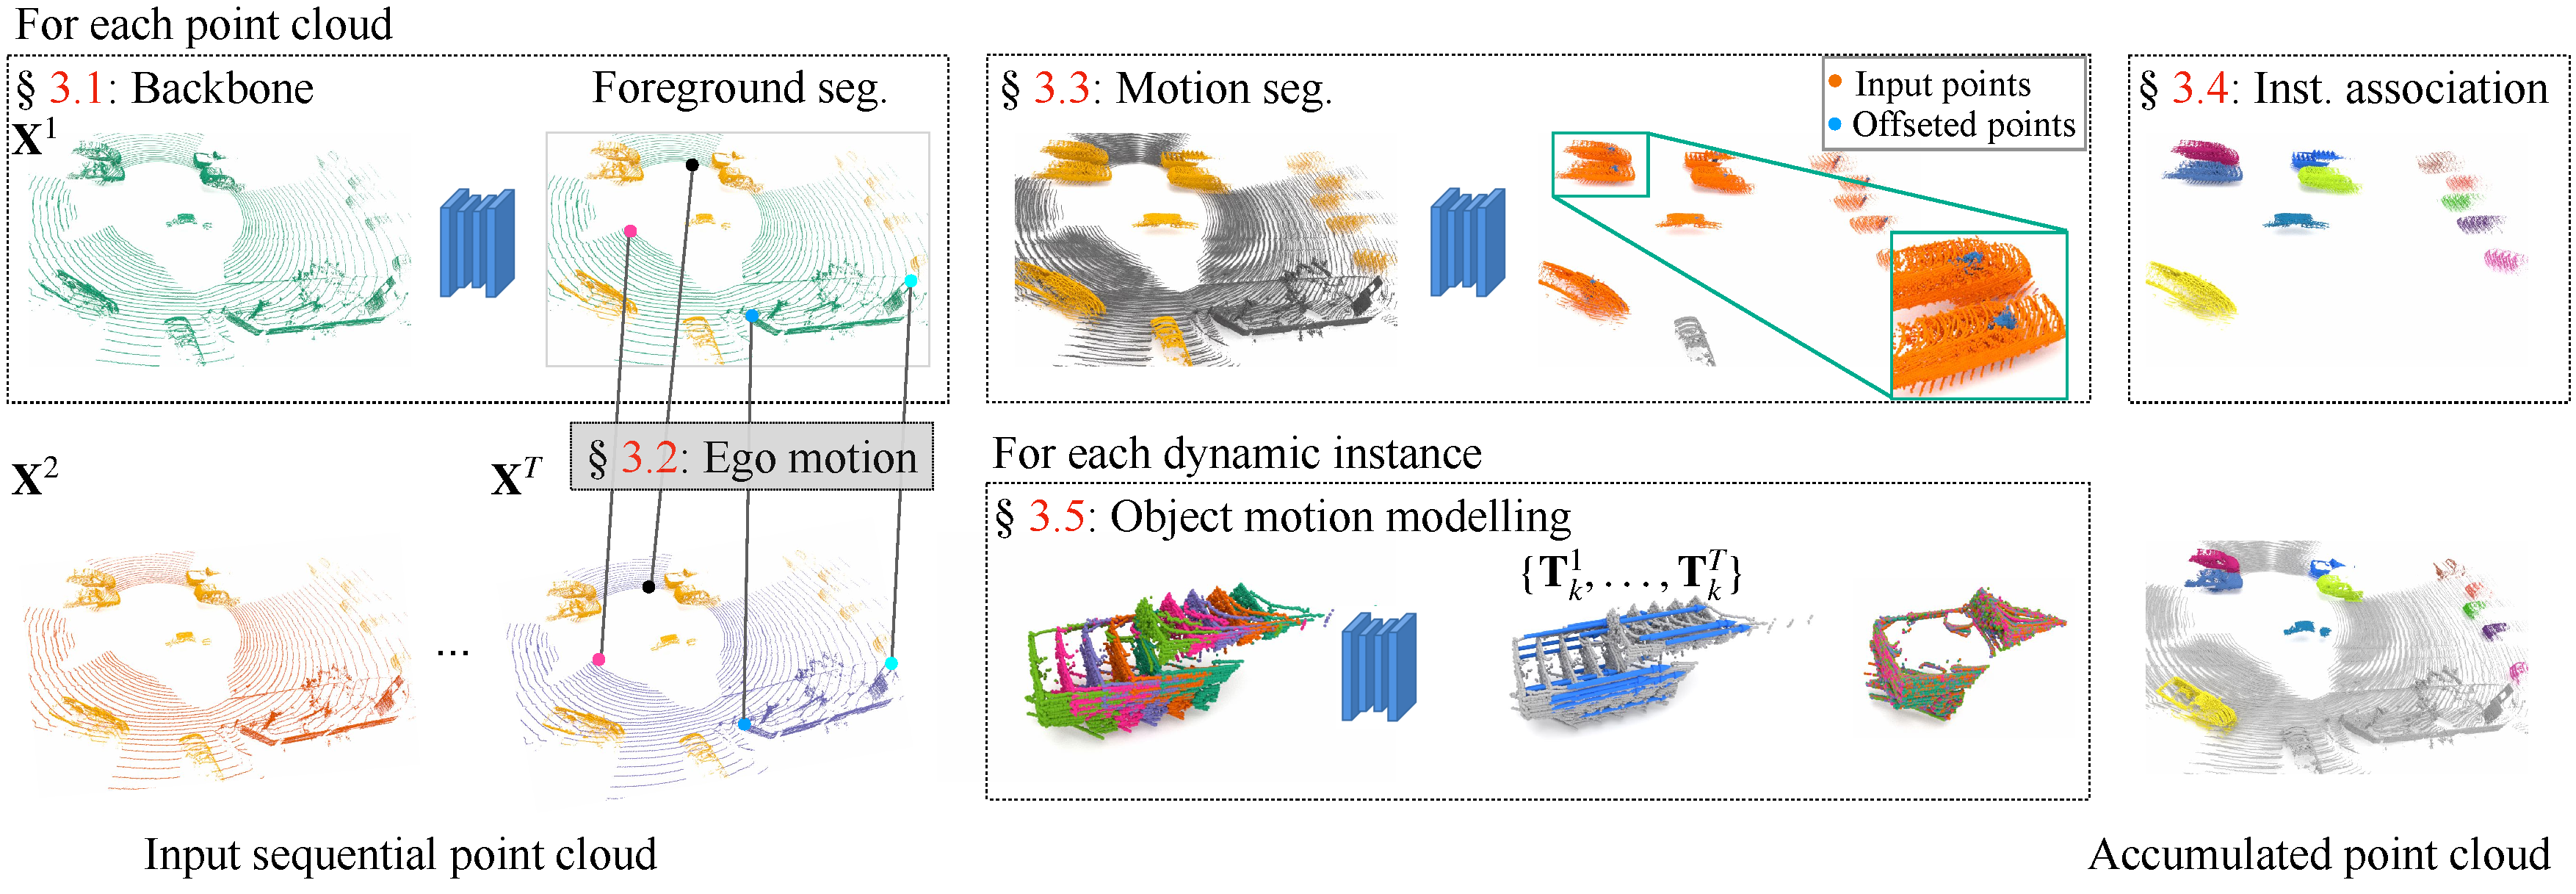
\includegraphics[width=1.0\textwidth]{Figures/overview.pdf}
        \caption{
        Overview of \dynfl. Our method takes LiDAR scans and tracked bounding boxes of dynamic vehicles as input. \dynfl first decomposes the scene into a static background and $N$ dynamic vehicles, each modelled using a dedicated neural field. These neural fields are then composed to re-simulate LiDAR scans in dynamic scenes. Our composition technique supports various scene edits, including altering object trajectories, removing and adding reconstructed neural assets between scenes.
    }
    \label{fig:main}
\end{figure*}

We introduce a neural representation for the purpose of reconstructing and manipulating LiDAR scans of dynamic driving scenes. 
Counterfactual re-simulation is an emerging application in the realm of autonomous driving, offering a unique approach to examining "what if" scenarios. This method involves creating a reconstruction of a real-world event, termed as \textit{digital twin} and then applying various modifications to it. These could include altering the environmental conditions, changing the action of some agent, or introducing additional scene elements. Analyzing the outcomes of these edited scenarios provides insights into the functioning of the perception system, moreover they can be used to obtain training data for rare situations.

The essence of counterfactual re-simulation is the capability to authentically recreate variations of the original, factual observation. We address this challenge in the context of LiDAR on autonomous vehicles (AV). Existing approaches to LiDAR re-simulation have important limitations. Conventional simulators such as CARLA~\cite{dosovitskiy2017carla} and NVIDIA DRIVE Sim are capable of modeling LiDAR sensors. However, their reliance on manually designed 3D simulation assets requires significant human effort. LiDARsim~\cite{manivasagam2020lidarsim} aims to remedy this by reconstructing vehicles and scenes from real measurements. While producing encouraging results, its two-stage LiDAR modeling lacks realism, particularly in terms of physical effects like multi-returns and reflected intensity, which were shown 
 to matter for downstream processing~\cite{guillard2022learning}. Following NeRF's~\cite{mildenhall2020nerf} success in camera view synthesis, some works have applied neural fields for LiDAR modeling~\cite{Huang2023nfl, tao2023lidar, zhang2023nerf}. In particular, Neural LiDAR Fields (NFL)\cite{Huang2023nfl} developed a physically inspired LiDAR volumetric rendering scheme that accounts for two-way transmittance and beam width, allowing faithful recovery of secondary returns, intensity, and ray drops. These models are, however, limited to static scenes that do not change while multiple input views are scanned, and are thus of limited use for re-simulation in the presence of moving traffic. Recently, UniSim~\cite{yang2023unisim} followed Neural Scene Graph~\cite{Ost_2021_CVPR} in modeling road scenes as sets of movable NeRF instances on top of a static background. UniSim introduced a unified synthesis approach for camera and LiDAR sensors, but ignored physical sensor properties like two-way transmittance and beam width~\cite{Huang2023nfl}.

We present \dynfl, a novel approach for re-simulating LiDAR views of driving scenarios. Our method builds upon a neural SDF that enables an accurate representation of scene geometry, while at the same time enforcing physical accuracy by modeling two-way transmittance, like NFL~\cite{Huang2023nfl}. 
% Our method builds upon UniSim's SDF representation and scene decomposition, but enhances the physical accuracy by incorporating two-way transmittance modeling, as introduced in NFL.
%
Our primary contribution is a method for compositing neural fields that accurately integrates LiDAR measurements from individual fields representing different scene assets. With the help of a ray drop test, we effectively manage occlusions and transparent surfaces. This not only ensures physical accuracy, but also facilitates the inclusion of assets reconstructed from a variety of static and dynamic scenes, thereby enhancing control over the simulated content. Our method bridges the gap between the physical fidelity of the re-simulation and flexible editing of dynamic scenes.
%
We validate \dynfl with both synthetic and real-world data, focusing on three key areas: \textit{(i)} high-quality view synthesis, \textit{(ii)} perceptual fidelity, and \textit{(iii)} asset manipulation. We find that our approach outperforms baseline models \wrt both range and intensity. Its synthetic outputs also show higher agreement with real scans in terms of object detection and segmentation. Furthermore, \dynfl enables not only removal, duplication and repositioning of assets within the same scene, but also the inclusion of assets reconstructed in other scenes, paving the way for new applications.


% In the rapidly evolving field of computer vision, novel view synthesis has become a groundbreaking technique, especially in the realm of image-based rendering. Pioneered by technologies like NeRF~\cite{mildenhall2020nerf}, it allows for the creation of photo-realistic views from a given set of data. However, the application of these principles to LiDAR data, which inherently deals with point clouds, introduces a complex set of challenges and opportunities that are distinct from traditional image-based approaches.

% Historically, methods like LiDARsim~\cite{manivasagam2020lidarsim} have paved the way for such advancements, yet they exhibit limitations. Specifically, LiDARsim operates by first extracting an explicit scene representation and then performing ray-surfel casting to synthesize LiDAR scans. This approach, while innovative, is susceptible to inaccuracies due to point cloud noise and typically results in lower reconstruction quality. This limitation leads to a significant domain gap when compared to ground truth LiDAR scans. Our previous work, Neural Lidar Fields (NFL)~\cite{Huang2023nfl}, marked a substantial improvement in modeling LiDAR scenes with neural fields and incorporating the physical characteristics of LiDAR beams. Despite its state-of-the-art performance in geometry reconstruction, NFL was limited to static scenes and did not address the complexities of dynamic environments.

% In dynamic scenarios, particularly in automotive or robotics contexts, capturing the constant motion of elements like vehicles and pedestrians is crucial. Our work seeks to bridge this gap by extending the principles of NFL to dynamic settings. Prior approaches that tackle the dynamic scenes, such as LiDARsim~\cite{manivasagam2020lidarsim}, have adopted a reconstruct-then-simulate process, resulting in inferior geometric fidelity. Meanwhile, other neural-fields-based explorations like Neural Scene Graph~\cite{Ost_2021_CVPR} and UniSim~\cite{yang2023unisim} focus on image-based rendering or sensor fusion, neglecting LiDAR-specific attributes.

% In this context, our work contributes in several ways:
% \textbf{1.)} Improved Geometry Quality: We adopt a Signed Distance Function (SDF)-based volume rendering approach, specifically tailored to the active sensor characteristics of LiDAR beam. This method acknowledges and leverages the intricacies of how LiDAR sensors capture data, resulting in reconstructions of higher fidelity and geometric accuracy.
% \textbf{2.)} Innovative Neural Fields Composition: Our methodology introduces a novel technique for the composition of multiple neural fields. This approach significantly enhances the rendering process, allowing for seamless integration and higher-quality synthesis of dynamic views.

% Our paper delves into the technicalities of Dynamic Neural LiDAR Fields, elaborating on the methods and innovations that enable the synthesis of dynamic views from LiDAR data. We present extensive experimental results that showcase the effectiveness of our approach in dynamic environments, illustrating how our contributions extend the applicability of neural LiDAR fields. Through this work, we provide a valuable resource for researchers in computer vision, contributing to the broader discourse on LiDAR novel view synthesis for dynamic scenes.


\section{Related work}
\paragraph{Neural radiance fields and volume rendering}
Neural Radiance Fields (NeRF)~\cite{mildenhall2020nerf} have demonstrated remarkable success in novel-view image synthesis through neural volume rendering. These fields are characterized by the weights of Multilayer Perceptrons (MLPs), which enable the retrieval of volume density and RGB colors at any specified point within the field for image compositing via volume rendering. Several studies~\cite{barron2021mip,barron2022mip,verbin2022ref,chen2022tensorf,fridovich2022plenoxels} have subsequently advanced NeRF's rendering quality by addressing challenges such as reducing aliasing artifacts~\cite{barron2021mip}, scaling to unbound large-scale scenarios~\cite{barron2022mip}, and capturing specular reflections on glossy surfaces~\cite{verbin2022ref}.
Certain works~\cite{chen2022tensorf,fridovich2022plenoxels,mueller2022instant,kerbl20233d} have explored more effective representations of radiance fields. TensorsRF~\cite{chen2022tensorf} employs multiple compact low-rank tensor components, such as vectors and matrices, to represent the radiance field. Plenoxels~\cite{fridovich2022plenoxels} accelerates NeRF training by replacing MLPs with explicit plenoptic elements stored in sparse voxels and factorizing appearance through spherical-harmonic functions.
M\"uller et al.~\cite{mueller2022instant} achieved a substantial acceleration in rendering speed by employing a representation that combines trainable multi-resolution hash encodings (MHE) with shared shallow MLP networks. Kerbel et al.~\cite{kerbl20233d} introduce a novel volume rendering method utilizing 3D Gaussians to represent the radiance field and rendering images based on visibility-aware splatting of 3D Gaussians.


\paragraph{Dynamic neural radiance fields} 
Neural fields \cite{xie2022neural} can be extended to represent dynamic scenes. On top of the \textit{canonical} scene representation, some methods~\cite{pumarola2020d, park2021nerfies, park2021hypernerf,yuan2021star} additionally model the 4D deformation fields. Meanwhile, some other works learn a space-time correlated~\cite{kplanes_2023, li2020neural, attal2023hyperreel, liu2023robust}, or decomposed~\cite{turki2023suds,wu2022d,yang2023emernerf} neural field to encode the 4D scenes, achieving fine-grained reconstruction of the geometry and the appearance.
%
Some other methods decompose the scene into static and dynamic parts, and model each dynamic actor with dedicated neural fields. 
Neural Scene Graph~\cite{Ost_2021_CVPR} and Panoptic Neural Fields~\cite{KunduCVPR2022PNF} treat every dynamic object in the scene as a node, and synthesize photo-realistic RGB images by jointly rendering from both dynamic nodes and static background. UniSim\cite{yang2023unisim} employs neural SDF representation to model dynamic scenes in driving scenarios, and render in a similar way to Neural Scene Graph~\cite{Ost_2021_CVPR}.


\paragraph{Neural surface representation}
A fundamental challenge for NeRF and its variants involves accurately recovering the underlying 3D surface from the implicit radiance field. Surfaces obtained by thresholding on the volume density of NeRF often exhibit noise~\cite{wang2021neus, yariv2021volume}. To address this, implicit surface representations like Occupancy~\cite{niemeyer2020differentiable, oechsle2021unisurf} and signed distance functions (SDF)~\cite{wang2021neus, yariv2021volume, yu2022monosdf, sun2022neural, wang2022hf, zuo2023incremental, li2023neuralangelo, wang2023neus2} in grid maps are commonly integrated into neural volume rendering techniques.

NeuS~\cite{wang2021neus} introduces a neural SDF representation for surface reconstruction, proposing an unbiased weight function for the appearance composition process in volume rendering. Similarly, VolSDF~\cite{yariv2021volume} models scenes with a neural SDF and incorporates the SDF into the volume rendering process, advocating a sampling strategy of the viewing ray to bound opacity approximation error. Neuralangelo~\cite{li2023neuralangelo} improves surface reconstruction using the multi-resolution hash encoding (MHE)~\cite{mueller2022instant} and SDF-based volume rendering~\cite{wang2021neus}. While these methods might deliver satisfying dense surface reconstructions, their training is time-consuming, taking hours for a single scene.
Voxurf~\cite{wu2022voxurf} offers a faster surface reconstruction method through a two-stage training procedure, recovering the coarse shape first and refining details later. Wang et al.~\cite{wang2023neus2} expedites NeuS training to several minutes by predicting SDFs through a pipeline composed of MHE and shallow MLPs.

Many works also incorporate distances measured by LiDAR as auxiliary information to constrain the radiance field. For instance, works~\cite{chang2023neural, wang2023neural} render depth by accumulating volume density and minimizing depth discrepancies between LiDAR and render depth during training. Rematas et al.~\cite{rematas2022urban} enforces empty space between the actual surface and the ray origin.


\paragraph{LiDAR simulation} 
While simulators like CARLA~\cite{dosovitskiy2017carla} and AirSim~\cite{shah2018airsim} can simulate LiDAR data, they suffer from expensive human annotation requirements and a notable sim-to-real gap due to limited rendering quality. Generative model-based methods for LiDAR synthesis~\cite{caccia2019deep,zyrianov2022learning} offer an alternative but often lack control and produce distorted geometries~\cite{li2023pcgen}.
Learning-based approaches~\cite{li2023pcgen,fang2020augmented,manivasagam2020lidarsim} try to enhance realism by transferring real scan properties to simulations. For example, \cite{guillard2022learning} uses a RINet trained on RGB and real LiDAR data to augment simulated scan qualities. LiDARsim~\cite{manivasagam2020lidarsim} employs ray-surfel casting with explicit disk surfels for more accurate simulations.
Huang et al.~\cite{Huang2023nfl} proposed Neural LiDAR Fields (NFL), combining neural fields with a physical LiDAR model for high-quality synthesis, although it's limited to static scenes and can produce noisy outputs due to its unconstrained volume density representation.
UniSim~\cite{yang2023unisim} constructs neural scene representations from realistic LiDAR and camera data, using SDF-based volume rendering for sensor measurement generation at novel viewpoints.


\section{Dynamic Neural Scene Representation}

\paragraph{Problem statement} 
Consider a set of LiDAR scans $\mathcal{X} = \{\mathbf{X}_t\}_{t=1}^T$ that have been compensated for ego-motion, along with tracked bounding boxes\footnote{We assume that the ground truth object detection and tracking annotations are available.} for dynamic vehicles $\mathcal{B} = \{\mathbf{B}_t^v\}_{v=1}^{N}$, where $T$ represents the total number of LiDAR scans, and $N$ is the count of dynamic vehicles. Each scan $\mathbf{X}_t$ is composed of $n_t$ rays, each ray $\mathbf{r}$ is described by the tuple $(\origin, \dir, \zeta, \intensity, \pdrop)$, where $\origin$ and $\dir$ denote the ray's origin and direction, $\zeta$ and $\intensity$ represent range and intensity values, and $\pdrop \in \{0,1\}$ indicates whether the ray is dropped or not due to insufficient returned radiant power.


The goal is to reconstruct the scene with a static-dynamic decomposed neural representation, that can enable the rendering of LiDAR scan $\mathbf{X}_{\text{tgt}}$ from novel viewpoint $\mathbf{T}_{\text{tgt}}$. This setup also facilitates various object manipulations, including altering object trajectories, and inserting or removing objects from the scene. The overview of our method is given in~\cref{fig:main}.

\subsection{Neural Scene Decomposition} \label{sec: decomposition}
We leverage the inductive bias that driving scenes can be decomposed into a static component and $N$ rigidly-moving dynamic components~\cite{huang2022dynamic,gojcic2021weakly}. Consequently, we establish $N+1$ neural fields. The neural field $\mathbf{F}_{\text{static}}$ is designated for the static component of the scene, capturing the unchanging background elements. Concurrently, the set of neural fields $\{\mathbf{F}^v\}_{v=1}^{N}$ is used to model the $N$ dynamic entities, specifically the vehicles in motion.



\paragraph{Neural field for static background} 
The static background is encoded into a neural field $\mathbf{F}_\text{static}: (\x, \dir) \mapsto (s, \intensity, \pdrop)$ that estimates the signed distance $s$, intensity $\intensity$, and ray drop probability $\pdrop \in [0,1]$ given the point coordinates $\x$ and the ray direction $\dir$. In practice, we first use a multi-resolution hash encoding (MRH)~\cite{mueller2022instant} to map each point to its positional feature $\posfeat \in \real^{32}$, and project the view direction onto the first 16 coefficients of the spherical harmonics basis, resulting in $\dirfeat$. Subsequently, we utilize three Multilayer Perceptrons (MLPs) to estimate the scene properties as follows:
\begin{equation}
(s, \geofeat) = f_s(\posfeat), \quad \intensity = f_{\intensity}(\rayfeat), \quad \pdrop = f_{\text{drop}}(\rayfeat).
\end{equation}
Here, $f_s, f_e,$ and $f_{\text{drop}}$ are three MLPs, $\rayfeat \in \mathbb{R}^{31}$ represents the ray feature and is constructed by concatenating the per-point geometric feature and the directional feature. The geometric feature is denoted as $\geofeat \in \mathbb{R}^{16}$. For more implementation details, please refer to the appendix. 

\begin{figure}[t]
    \centering
        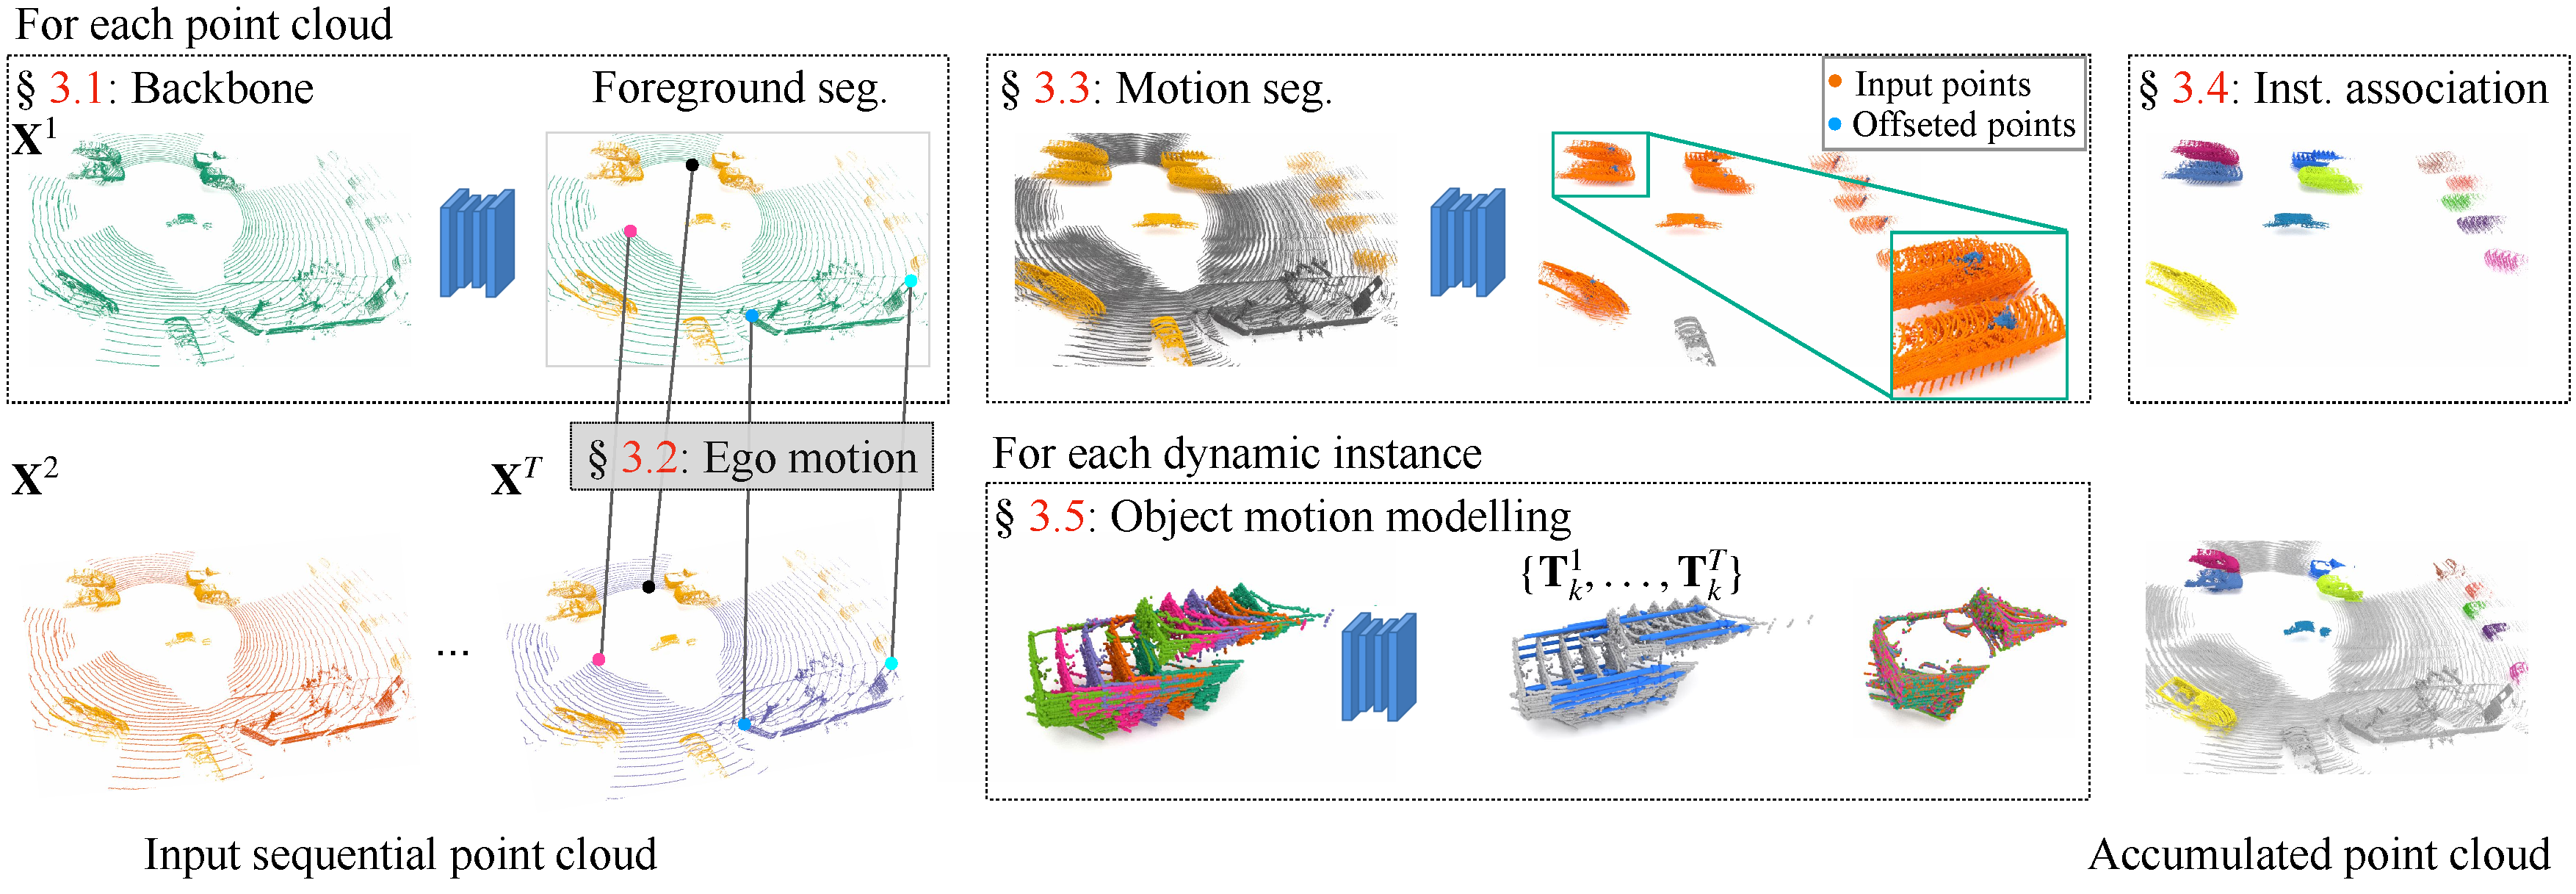
\includegraphics[width=1.0\columnwidth]{Figures/overview.pdf}
        \caption{
        Overview of \dynfl. Our method takes LiDAR scans and tracked bounding boxes of dynamic vehicles as input. \dynfl first decomposes the scene into a static background and $N$ dynamic vehicles, each modelled using a dedicated neural field. These neural fields are then composed to re-simulate LiDAR scans in dynamic scenes. Our composition technique supports various scene edits, including altering object trajectories, removing and adding reconstructed neural assets between scenes.
    }
    \label{fig:main}
\end{figure}


\paragraph{Neural fields for dynamic vehicles} 
LiDAR scans collected over time are often mis-aligned due to the motion of both the sensor and other objects in the scene. Despite applying ego-motion for aligning static background points, dynamic object points remain blurred along their trajectories. Our approach to constructing a dynamic neural scene representation is grounded in the assumption that each dynamic object only undergoes rigid motion. Therefore, we can first align them over time and reconstruct them in their \textit{canonical} coordinate frame, and then render them over time by reversing the alignment of the neural field.

Specifically, consider a dynamic vehicle $v$ 
occurring in LiDAR scans $\{\mathbf{X}^v_t\}_{t=1}^{T}$ along with the associated bounding boxes $\{\mathbf{B}^v_t \in \mathbb{R}^{3\times 8}\}_{t=1}^{T}$ in the world coordinate framework. Here each bounding box is defined by its eight corners, and the first bounding box $\mathbf{B}^v_1$ is considered as the \textit{canonical} box. We estimate the relative transformations $\{\mathbf{T}_t \in \text{SE}(3)\}_{t=2}^{T}$ between the remaining $T-1$ bounding boxes and the canonical box, expressed as $\mathbf{B}_1^v = \mathbf{T}_t \mathbf{B}_t^v$\footnote{$\mathbf{T}\mathbf{B} = \mathbf{R}\mathbf{B} + \mathbf{t}$, where $\mathbf{R}$ and $\mathbf{t}$ are the rotation and translation components of $\mathbf{T}$.}. 
Subsequently, all LiDAR measurements on the object are transformed and accumulated in its canonical coordinate frame. The vehicle $v$ is then reconstructed in its canonical space, akin to the static background, using a neural field $\mathbf{F}^v$. To render the dynamic vehicle at timestamp $t$, the corresponding rigid transformation is applied to the queried rays. The dynamic neural field can thus be expressed as: $\mathbf{F}^v_t: (\mathbf{T}_{t}\x, \mathbf{T}_{t}\dir) \mapsto (s, \intensity, \pdrop)$. The rendering process for $\mathbf{F}^v$ is the same as rendering for static neural field $\mathbf{F}_{\text{static}}$.



\section{Neural rendering of the dynamic scene}
In this section, we present the methodology for rendering LiDAR scans from the neural scene representation. We begin by revisiting the density-based volume rendering formulation for active sensors~\cite{Huang2023nfl} in \cref{sec:vol_render_background}. Subsequently, we explore the extension of this formulation to SDF-based neural scene representation in \cref{sec:sdf_vol_render}. Finally, we provide a detailed discussion on rendering LiDAR measurements from individual neural fields in~\cref{sec:dynamic_nfl_rendering} and the process of composing results from different neural fields in \cref{sec:neural_fields_composition}.



\subsection{Volume rendering for active sensor} 
\label{sec:vol_render_background}
LiDAR utilizes laser beam pulses to determine the distance to the nearest reflective surface by analyzing full waveform profile of the returned radiant power. The radiant power $P(\zeta)$ from range $\zeta$ is the result of a convolution between the pulse power $P_e(t)$ and the impulse response $H(\zeta)$, defined as~\cite{hahner2021fog,hahner2022lidar,Huang2023nfl}:
\begin{equation}
    P(\zeta) = \int_0^{2\zeta/c} P_e(t) H(\zeta - \frac{ct}{2}) \; dt\;.
\label{eq:lidar}
\end{equation}
The impulse response $H(\zeta)$ is a product of the target and sensor impulse responses: $H(\zeta) = H_T(\zeta)\cdot H_S(\zeta)$, and the individual components are expressed as:
\begin{equation}
    H_T(\zeta) = \frac{\reflectance}{\pi} \cos(\theta) \delta(\zeta - \bar{\zeta})\;, \quad  H_s(\zeta) = \transmittance^2_{\zeta} \frac{A_e}{\zeta^2}\;,
\label{eq:ht}
\end{equation}
where $\reflectance$ represents the surface reflectance, $\theta$ denotes incidence angle, $\bar{\zeta}$ is the ground truth distance to the nearest reflective surface, $\transmittance_{\zeta}$ and $A_e$ describe the transmittance at range $\zeta$ and sensor's effective area, respectively. Due to the non-differentiability introduced by the indicator function $\delta(\zeta - \bar{\zeta})$, ~\cref{eq:lidar} is non-differentiable and is thus not suitable for solving the inverse problem. NFL~\cite{Huang2023nfl} solves it by extending it into a probabilistic formulation given by:
\begin{equation}
P(\zeta) = C \cdot \frac{T^2_{\zeta} \cdot \density_\zeta  \reflectance_\zeta}{\zeta^2} \cos(\theta)\;.
\label{eq:radiance}
\end{equation}
Here, $C$ accounts for the constant values, and $\sigma_\zeta$ represents the density at range $\zeta$. The radiant can be reconstructed using the volume rendering formulation:
\begin{equation}
      P
      =\!\sum_{j=1}^N \int_{\zeta_j}^{\zeta_{j+1}}\!\!C \frac{\transmittance^2_{\zeta} \cdot \density_\zeta \reflectance_\zeta}{\zeta^2} \cos(\theta_j) \; d\zeta
      =\!\sum_{j=1}^N w_j \reflectance_{\zeta_j}',
\label{eq:radiant_inter}
\end{equation}
where the weights $w_j = 2 \opacity_{\zeta_j} \cdot\prod_{i=1}^{j-1}(1 - 2 \opacity_{\zeta_i}).$
Here $\alpha_{\zeta_j}$ is the discrete opacity at range $\zeta_j$. Please refer to~\cite{Huang2023nfl} for more details.


\subsection{SDF-based volume rendering for active sensor} 
\label{sec:sdf_vol_render}
A neural scene representation based on probabilistic density often results in surfaces with noticeable noise due to insufficient surface regularization~\cite{wang2021neus}. To address this, we opt for a signed distance-based scene representation and establish the volume rendering formulation within the framework of an active sensor. Building upon SDF-based volume rendering for passive sensors~\cite{wang2021neus}, we compute the opaque density $\tilde{\density}_{\zeta_i}$ as follows:
\begin{equation}
\tilde{\density}_{\zeta_i} = \max\left(\frac{-\frac{{\textrm{d}}\Phi_s}{{\textrm{d}} \zeta_i}(f(\zeta_i))}{\Phi_s(f(\zeta_i))},0\right),
\label{eq:sigmoid_density}
\end{equation}
where $\Phi_s(\cdot)$ represents the Sigmoid function, $f(\zeta)$ evaluates the signed distance to the surface at range $\zeta$ along the ray $\ray$. 

Next, we substitute the density $\density$ in \cref{eq:radiant_inter} with opaque density from \cref{eq:sigmoid_density} and re-evaluate the radiant power and weights as:
\begin{equation}
      P
      =\!\sum_{j=1}^N \transmittance^2_{\zeta_j} \tilde{\alpha}_{\zeta_j} \reflectance_{\zeta_j}',\quad \tilde{w}_j = 2 \tilde{\opacity}_{\zeta_j} \cdot\prod_{i=1}^{j-1}(1 - 2 \tilde{\opacity}_{\zeta_i})\;.
\end{equation}
In this context, $\tilde{\alpha}_{\zeta_j}$ is computed as:
\begin{equation}
    \tilde{\alpha}_{\zeta_j} = \max\left(\!\frac{{\Phi_s(f(\zeta_j))}^2 -{\Phi_s(f(\zeta_{j+1}))}^2}{{2\Phi_s(f(\zeta_j))}^2},0\right).
    \label{eq:new_weights}
\end{equation}
Please refer to the appendix for more details.


\subsection{Volume rendering for LiDAR measurements}
\label{sec:dynamic_nfl_rendering}
Consider rendering the LiDAR measurements from a single neural field, we employ the hierarchical sampling\cite{wang2021neus} technique to sample a total of $N_s= N_u + N_i$ points along each ray, where $N_u$ points are uniformly sampled, and $N_i$ points are probabilistically sampled based on the weights along the ray, facilitating denser sampling in proximity to the surface. Subsequently, we compute the weights for the $N_s$ points following~\cref{eq:new_weights}. The rendering of range, intensity, and ray drop for each ray can be expressed through volume rendering as follows: $y_\text{est} = \sum_{j=1}^{N_s} w_j y_j$, where $y \in \{\zeta, \intensity, \pdrop\}$.


\subsection{Neural rendering for multiple fields}\label{sec:neural_fields_composition}
Our full neural scene representation comprises $N+1$ neural fields as discussed in ~\cref{sec: decomposition}. Rendering from all these fields for each ray during inference is computationally intensive. To address this, we implement a two-stage method. In the first stage, we identify the $k+1$ neural fields, where $k \geq 0$ represents the number of dynamic fields, that are likely to intersect with a given ray. The second stage involves rendering LiDAR measurements from these selected fields individually and then integrating them into a unified set of measurements.


\paragraph{Ray intersection test}
As outlined in~\cref{sec: decomposition}, each dynamic neural field is reconstructed in its unique canonical space, defined by a corresponding canonical box. To determine neural fields intersecting with a ray at inference time, we begin by estimating the transformations $\{\mathbf{T}_t^v\}_{v=1}^N$, which convert coordinates from the world framework to each vehicle's canonical space at timestamp $t$. These transformations are determined by interpolating the training set transformations using spherical linear interpolation (SLERP)~\cite{10.1145/325334.325242}. Following this, we apply transformations to the queried ray and run intersection tests with the canonical boxes of the scenes. 


\paragraph{Neural rendering from multiple neural fields}
 After identifying the $k+1$ neural fields that potentially intersect with a ray, we perform volume rendering on each field separately, yielding $k+1$ distinct sets of LiDAR measurements. Next, we evaluate the ray drop probabilities across these fields. A ray is deemed \textit{dropped} if all neural fields indicate a drop probability $\pdrop > 0.5$. For rays not classified as dropped, we sort the estimated ranges in ascending order and select the nearest one as our final range prediction. Correspondingly, the intensity value is extracted from the same neural field associated with this closest range.

\section{Neural Scene Optimisation} \label{sec:optmisation}
Given the set of LiDAR scans and the associated tracked bounding boxes of the dynamic vehicles, we optimise our neural scene representation by minimising the loss:
\begin{equation}
    \mathcal{L} = w_{\zeta} \mathcal{L}_{\zeta} +  w_{s} \mathcal{L}_{s} + w_{\text{eik}} \mathcal{L}_{\text{eik}} + w_{\intensity} \mathcal{L}_{\intensity} + w_{\text{drop}} \mathcal{L}_{\text{drop}},
    \label{loss}
\end{equation}
where $w_{*}$ denotes respective weights, and each individual loss term $\mathcal{L}_*$ is explained below.


\paragraph{Range reconstruction loss}
For range estimation, we employ L1 loss, defined as: $\mathcal{L}_{\zeta} = \frac{1}{|\mathcal{R}|}\sum_{\ray \in \mathcal{R}}|\zeta_{est} -\zeta_{gt}|$, where $\mathcal{R}$ denotes the set of LiDAR rays, $\zeta_{est}$ and $\zeta_{gt}$ correspond to the estimated and actual ranges, respectively. 


\paragraph{Surface points' SDF regularisation} \label{sec:surfacesdf}
Acknowledging that LiDAR points mostly come from actual surface, we introduce an additional SDF regularisation term $\mathcal{L}_{s}$ that penalizes surface points' SDF values: $\mathcal{L}_{s} = \frac{1}{|\mathcal{P}|}\sum_{\mathbf{p} \in \mathcal{P}}|s(\mathbf{p})|$. Here $\mathcal{P}$ denotes the set of surface points and $s({\mathbf{p}})$ represents the SDF value of the point $\mathbf{p}$.


\paragraph{Eikonal constraint}
Following~\cite{icml2020_2086}, we utilize the Eikonal loss, $\leik$, to regularize the SDF level set. This ensures the gradient norm of the SDF is approximately one at any queried point. The loss is computed as: $\leik = \frac{1}{|\mathcal{Z}|} \sum_{\mathbf{p} \in \mathcal{Z}}( \| \nabla s(\mathbf{p}) \|_2 - 1)^2$, where $\mathcal{Z}$ is the set of all the sampled points. To stablise the training procedure, we adopt a numerical approach~\cite{li2023neuralangelo} to compute $\nabla s(\pos)$ as: 
\begin{equation}
    \nabla s(\pos) = \frac{s \left( \pos + \boldsymbol{\epsilon} \right) - s \left(\pos - \boldsymbol{\epsilon} \right)}{2 \epsilon} \;,
    \label{eqn:central_diff_normal}
\end{equation}
where the numerical step size $\epsilon$ is set to be $10^{-3}$ meters.


\paragraph{Intensity Loss}
For intensity reconstruction, we apply L2 loss, defined as: $\mathcal{L}_{\intensity} = \frac{1}{|\mathcal{R}|}\sum_{\ray \in \mathcal{R}}(\intensity_{est} -\intensity_{gt})^2.$


\paragraph{Ray drop loss}
We follow~\cite{Huang2023nfl} to supervise the ray drop estimation with a combination of a binary cross entropy loss $\mathcal{L}_{bce}$ and a Lovasz loss $\mathcal{L}_{ls}$ \cite{berman2018lovasz} as:
\begin{equation}
     \mathcal{L}_{\text{drop}} = \frac{1}{|\mathcal{R}|} \sum_{\ray \in \mathcal{R}} \left(\mathcal{L}_{bce}(p_{d, est}, {p_{d, gt}}) + \mathcal{L}_{ls}(p_{d, est}, {p_{d, gt}}) \right)\;.
     \label{eq:raydrop_loss}
\end{equation}
It's worth noting that in the context of dynamic neural fields, during training, we incorporate all LiDAR rays that intersect with the objects' bounding boxes of the scenes. A ray is classified as \textit{dropped} either if it is labeled as such in the dataset or if it does not intersect with the actual surfaces of the dynamic vehicles (\eg rays that are close but in parallel to the surfaces). This approach enhances the accuracy and realism of the reconstructed dynamic neural fields, improving the rendering fidelity at inference time. 

\section{Experiments}
\begin{figure*}[t]
  \centering
   \includegraphics[width=1\textwidth]{Figures/errormap_dynamic_3.pdf}
   
   \caption{Qualitative comparison of range estimation on \textit{Waymo Dynamic} dataset. Dynamic vehicles are zoomed in, and points are color-coded by range errors~(-100 \bwrDyNFL~100 cm).
   }
   \label{fig:errormap_dynamic}
   
\end{figure*}








\subsection{Datasets and Evaluation Protocol}\label{sec:datasets}

\paragraph{Real-world dynamic scenes} 
We construct \textit{Waymo Dynamic} dataset by selecting four representative scenes from Waymo Open dataset~\cite{sun2020scalability}, with multiple moving vehicles inside. These scenes are comprised of sequences of 50 consecutive frames. For evaluation purposes, every fifth frame is designated for testing, while the other 40 frames are allocated for training.


\paragraph{Real-world static scenes}
We also evaluate our method on four static scenes as introduced in~\cite{Huang2023nfl}. There are two settings, \textit{Waymo Interp} applies the same evaluation protocol as \textit{Waymo Dynamic}, while \textit{Waymo NVS} employs a dedicated closed-loop evaluation to validate the real novel view synthesis performance. Please refer to NFL~\cite{Huang2023nfl} for more details about this setting. 
 


\paragraph{Synthetic static scenes}  
\textit{TownClean} and \textit{TownReal} are synthetic static scenes introduced in NFL~\cite{Huang2023nfl}. They consist of 50 LiDAR scans simulated in urban street environment, using non-diverging and diverging beams, respectively. 



\paragraph{Evaluation metrics}\label{sec:metrics}
To evaluate the LiDAR range accuracy, we employ a suite of four metrics: mean absolute errors~(MAE [cm]), median absolute errors~(MedAE [cm]), Chamfer distance~(CD[cm]) and MedAE for dynamic vehicles~(MedAE Dyn[cm]). For intensity evaluation, We report root mean square error~(RMSE).
%
In addition to our primary evaluations, we assess the re-simulated LiDAR scans' realism through two auxiliary tasks: object detection and semantic segmentation. For object detection, we calculate the \textit{detection agreement}~\cite{manivasagam2020lidarsim}, both for all vehicles (Agg.~[\%]) and specifically for dynamic vehicles (Dyn.$\;$Agg.~[\%]). Regarding semantic segmentation, we measure and report recall, precision, and the intersection over union (IoU[\%]). It's important to note that the predictions on the original LiDAR scans serve as our \textit{ground truth}, against which we compare the results obtained from the re-simulated scans.




\paragraph{Baseline methods}
Regarding LiDAR simulation on static scenes, NFL~\cite{Huang2023nfl} and LiDARsim\cite{manivasagam2020lidarsim} are two closest baselines to compare to. Additionally, we include i-NGP~\cite{mueller2022instant}, DS-NeRF~\cite{kangle2021dsnerf}, and URF~\cite{rematas2022urban} for comparison. As for simulation on dynamic scenes, we compare to LiDARsim~\cite{manivasagam2020lidarsim} and UniSim~\cite{yang2023unisim}\footnote{We re-implement LiDARsim~\cite{lee2015lidar} and UniSim~\cite{yang2023unisim} as they are not open-sourced.}. Please refer to the appendix for implementation details.


\begin{table}[t]
    \setlength{\tabcolsep}{4pt}
    \renewcommand{\arraystretch}{1.2}
	\centering
	\resizebox{\columnwidth}{!}{
    \begin{tabular}{l|ccccc}
    \toprule
    Method  & MAE $\downarrow$ &  MedAE $\downarrow$ & CD $\downarrow$ & MedAE Dyn $\downarrow$ & Intensity RMSE $\downarrow$\\
    \midrule
    LiDARsim~\cite{manivasagam2020lidarsim} & 170.1 & 11.5 & 31.1 &  16.0  & 0.10\\
    Unisim~\cite{yang2023unisim} & 35.6 & 6.1 & 14.3 &14.3 & \textbf{0.05}\\
    Ours~ & \textbf{30.8} & \textbf{3.0} & \textbf{10.9} &\textbf{8.5} & \textbf{0.05}\\
    \bottomrule
    \end{tabular}
    }
    
	\caption{Evaluation of LiDAR NVS on \textit{Waymo Dynamic} dataset.}
	\label{tab:waymodynamic}
\end{table}
\begin{table}[t]
    \setlength{\tabcolsep}{4pt}
    \renewcommand{\arraystretch}{1.2}
	\centering
	\resizebox{\columnwidth}{!}{
    \begin{tabular}{l|ccc|ccc|ccc|ccc}
    \toprule
    & \multicolumn{3}{c|}{TownClean}& \multicolumn{3}{c|}{TownReal} & \multicolumn{3}{c|}{Waymo interp.} & \multicolumn{3}{c}{Waymo NVS} \\
    Method  & MAE $\downarrow$ &  MedAE $\downarrow$ & CD $\downarrow$& MAE $\downarrow$ &  MedAE $\downarrow$ & CD $\downarrow$ & MAE $\downarrow$ &  MedAE $\downarrow$ & CD $\downarrow$ & MAE $\downarrow$ &  MedAE $\downarrow$ & CD $\downarrow$\\
    \midrule
    i-NGP~\cite{mueller2022instant} &42.2 &4.1 & 17.4 & 49.8 & 4.8 & 19.9 & \textbf{26.4} & 5.5 & \textbf{11.6} & \underline{30.4} & 7.3 & 15.3\\
    DS-NeRF~\cite{kangle2021dsnerf} &41.7 & 3.9 &16.6 & 48.9 & 4.4 & 18.8 & \underline{28.2} & 6.3 & 14.5 & 30.4 & 7.2 & 16.8 \\
    URF~\cite{rematas2022urban} &43.3&4.2&16.8& 52.1 & 5.1 & 20.7 & 28.2 & 5.4 & 12.9 & 43.1 & 10.0 & 21.2 \\
    LiDARsim~\cite{manivasagam2020lidarsim} &159.6&\underline{0.8}&23.5& 162.8 & 3.8 & 27.4 & 116.3 & 15.2 & 27.6 & 160.2 & 16.2 & 34.7 \\
    NFL\cite{Huang2023nfl}  &\underline{32.0}&2.3&\underline{9.0}& \underline{39.2} & \underline{3.0} & \underline{11.5} & 30.8 & \underline{5.1} & \underline{12.1}& 32.6 & \underline{5.5} & \underline{13.2}  \\
    Ours & \textbf{26.7} & \textbf{0.7} & \textbf{6.7} &\textbf{33.9}&\textbf{2.1}&\textbf{10.4}& 28.3 & \textbf{4.7} & 12.5 & \textbf{28.6} & \textbf{4.9} & \textbf{13.0} \\
    \bottomrule
    \end{tabular}
}
    
	\caption{Evaluation of LiDAR NVS on static scenes.}
	\label{tab:waymostatic}
\end{table}
\begin{figure}[t]
  \centering
   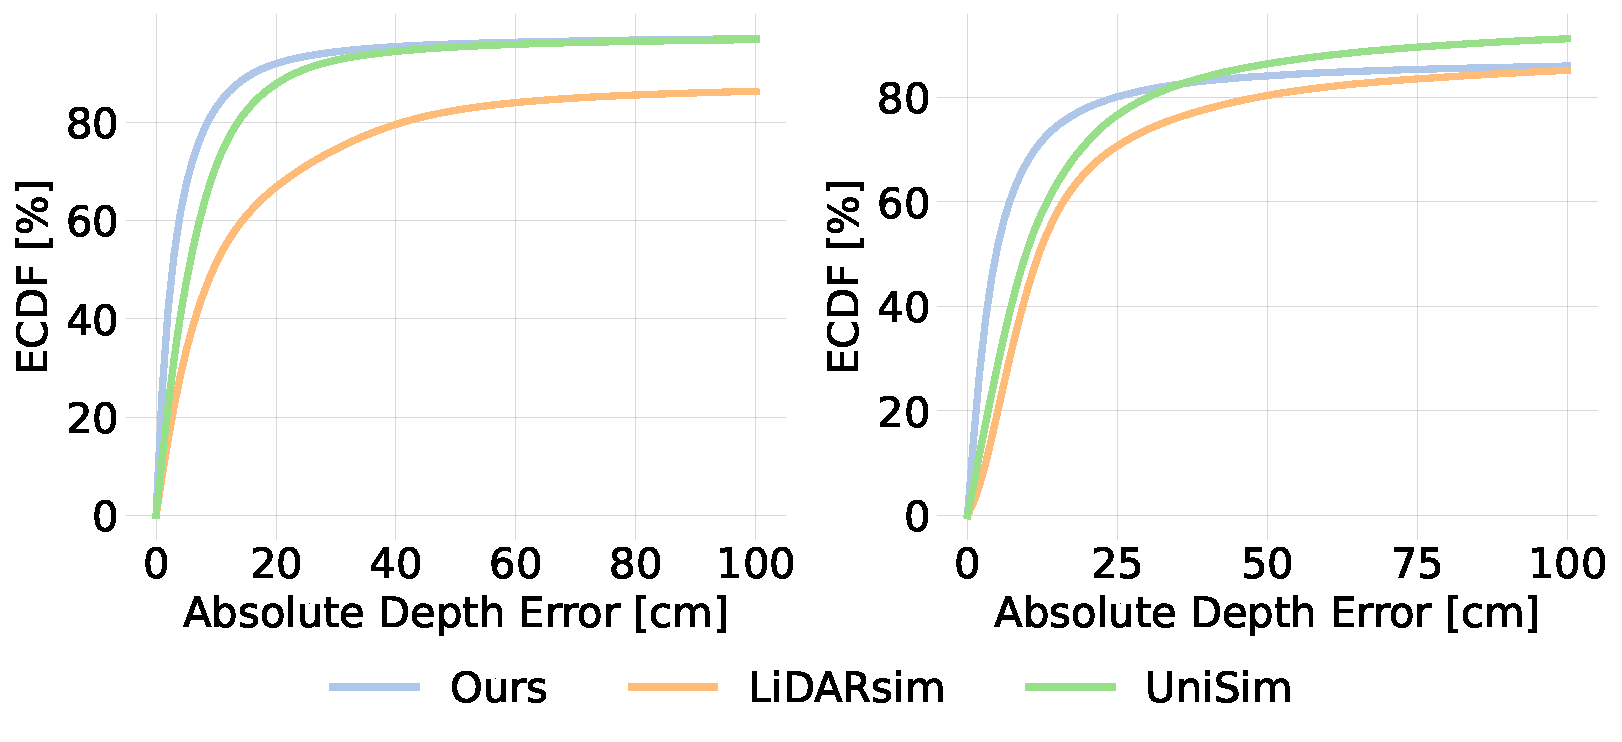
\includegraphics[width=1\columnwidth]{Figures/ecdf_3_methods.pdf}
   
        \caption{ECDF plots showcasing range errors across all the points (left) and specifically for points associated with dynamic vehicles (right). Our neural fields composition demonstrates superior performance over LiDARsim~\cite{manivasagam2020lidarsim} and UniSim~\cite{yang2023unisim}, especially in the context of dynamic vehicles.}
   \label{fig:ecdf}
   
\end{figure}
\begin{figure}[t]
    \centering
        \includegraphics[width=1\columnwidth]{Figures/errormap_static.pdf}
        
        \caption{Qualitative results of range estimation. Regions with gross errors (-100 \bwrDyNFL~100 cm) are highlighted.
        }
    \label{fig:error_map}
\end{figure}
\subsection{LiDAR Novel View Synthesis Evaluation} \label{sec:lidar_eval}
\paragraph{LiDAR NVS in dynamic scenes}
Quantitative comparisons with baseline methods are detailed in~\cref{tab:waymodynamic}. \dynfl notably outperforms LiDARsim~\cite{manivasagam2020lidarsim} and UniSim~\cite{yang2023unisim} in range reconstruction. This improvement is largely due to our SDF-based neural scene representation, which incorporates the physical aspects of LiDAR sensing. Additionally, our method employs a ray drop test when rendering multiple neural fields, leading to a more accurate reconstruction of dynamic vehicles, as evidenced in~\cref{fig:errormap_dynamic} and further supported by the data in~\cref{fig:ecdf}.


\begin{figure*}[t]
    \centering
        \includegraphics[width=1.0\textwidth]
        {Figures/sensor_manipulation.pdf}
        
        \caption{LiDAR novel view synthesis by changing sensor elevation angle~($\theta$), poses~($x,y,z$) and number of beams on \textit{Waymo Dynamic} dataset. The points are color-coded by the intensity values (0 \bwrDyNFL~0.25).}
    \label{fig:lidar_nvs}
\end{figure*}
\paragraph{LiDAR NVS in static scenes}
In addition to dynamic scenes, we evaluate \dynfl against baseline methods in static scenarios, with the results detailed in~\cref{tab:waymostatic} and~\cref{fig:error_map}. \dynfl excels in reconstructing geometry in most cases. A key observation is its superior performance in reconstructing planar regions (\eg the ground shown in~\cref{fig:error_map}), especially when compared to NFL~\cite{Huang2023nfl}, which also uses a neural field for surface representation. This improvement is largely due to the enhanced surface regularizations provided by our advanced SDF-based surface modeling approach.


\begin{table}[t]
    \setlength{\tabcolsep}{4pt}
    \renewcommand{\arraystretch}{1.2}
	\centering
	\resizebox{0.5\columnwidth}{!}{
    \small
    \begin{tabular}{l|ccc}
    \toprule
    Datasets  & MAE $\downarrow$ &  MedAE $\downarrow$ & CD $\downarrow$ \\
    \midrule
    TownClean~ & 26.7(\textcolor{green}{-1.5}) & 0.7(\textcolor{green}{-0.2}) & 6.7(\textcolor{green}{-0.5})\\
    Waymo Interp~ & 28.3 (\textcolor{red}{0.1}) & 4.7 (\textcolor{green}{-0.2}) & 12.5 (\textcolor{green}{-0.1})\\
    Waymo Dynamic~ & 30.8 (\textcolor{green}{-0.3}) & 3.0 (\textcolor{green}{-0.2}) & 10.9 (\textcolor{green}{-0.3})\\
    \bottomrule
    \end{tabular}
    }
    
	\caption{Ablation study of volume rendering for active sensing.}
	\label{tab:active_sensing}
\end{table}
\begin{table}[t]
    \setlength{\tabcolsep}{4pt}
    \renewcommand{\arraystretch}{1.2}
	\centering
	\resizebox{0.5\columnwidth}{!}{
    \small
    \begin{tabular}{l|ccc}
    \toprule
    Datasets  & MAE $\downarrow$ &  MedAE $\downarrow$ & CD $\downarrow$ \\
    \midrule
    TownReal~ & 33.9(\textcolor{green}{-3.3}) & 2.1(\textcolor{green}{-0.0}) & 10.4(\textcolor{green}{-1.2})\\
    Waymo Interp~ & 28.3 (\textcolor{green}{-0.3}) & 4.7 (\textcolor{green}{-0.1}) & 12.5 (\textcolor{green}{-0.3})\\
    \bottomrule
    \end{tabular}
    }
    
	\caption{Ablation study of the surface points' SDF regularisation.}
	\label{tab:surface_sdf}
\end{table}
\begin{figure}[t]
  \centering
   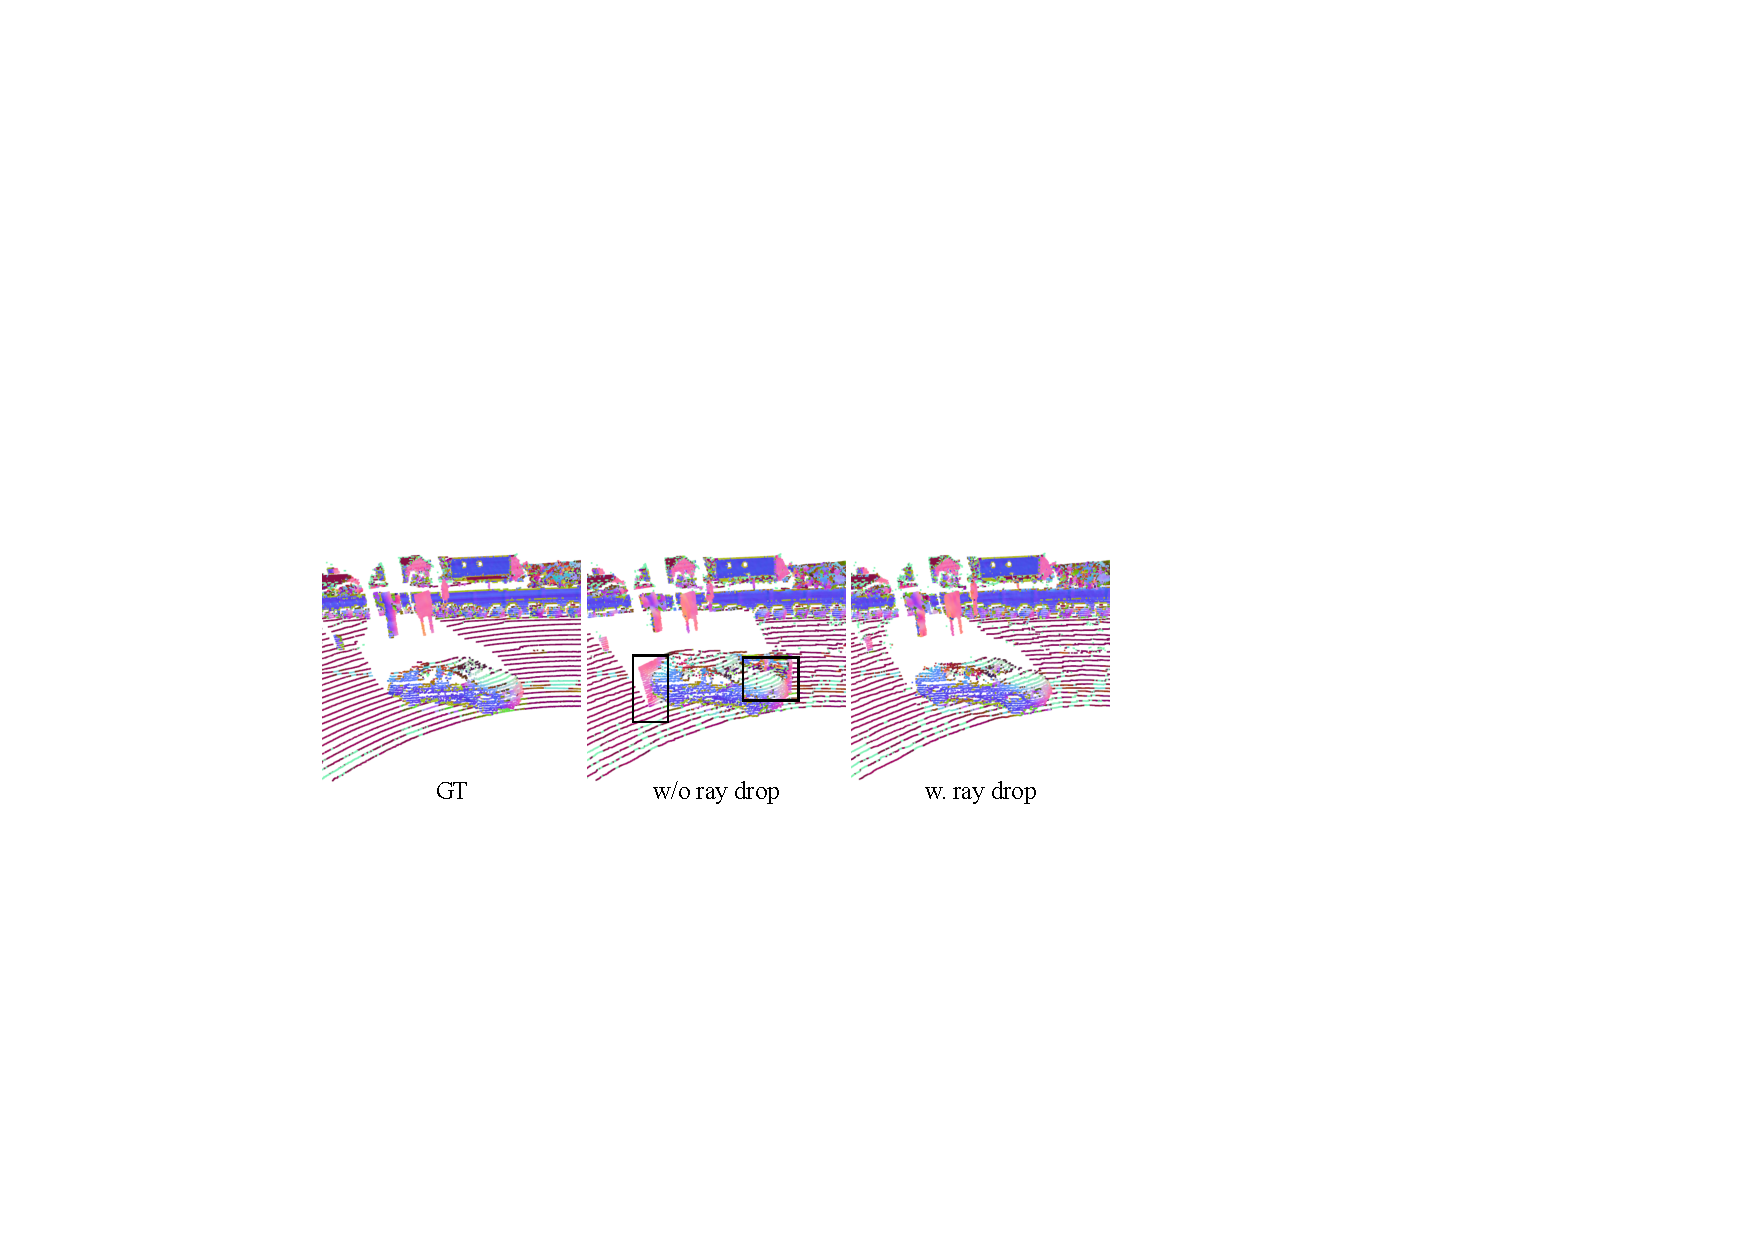
\includegraphics[width=1\linewidth]{Figures/intersectiontest.pdf}
   
   \caption{
   Qualitative results on \textit{Waymo Dynamic} dataset. Our model equipped with a ray drop module effectively composites multiple neural fields, re-simulating LiDAR scans of high quality.
   }
   % \caption{These figures exemplify the effectiveness of our field composition method leveraging ray drop probability from dynamic neural field. When all intersected rays are rendered for the dynamic neural field, noticeable artifacts appear due to disturbances from irrelevant fields (middle figure). The figures on the right showcase the complete composition method.
   % }
   % \caption{
   % }
    
   \label{fig:ablation_raydrop}
\end{figure}

\begin{figure}[t]
    \centering
        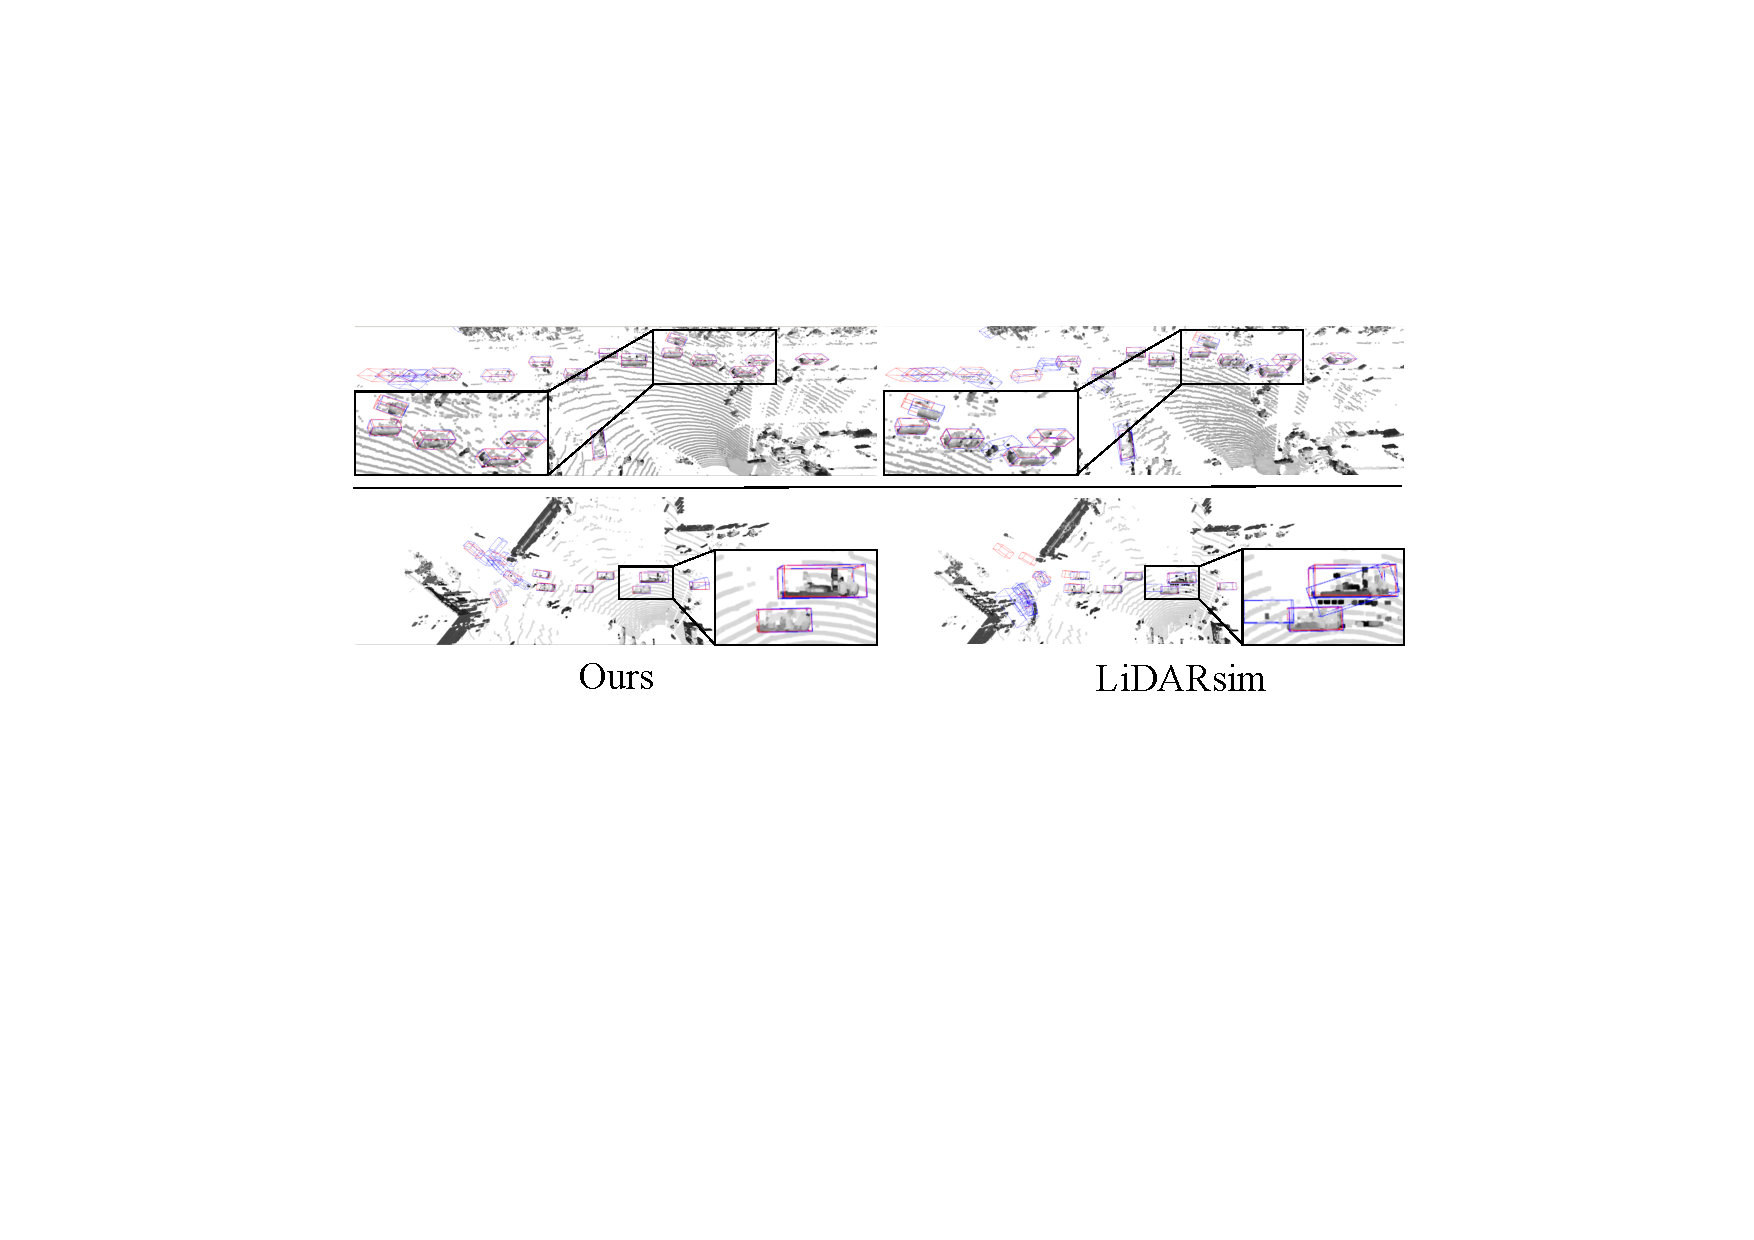
\includegraphics[width=0.8\columnwidth]{Figures/detection_result.pdf}
        \caption{Object detection results on \textit{Waymo Dynamic} dataset. The ground truth and predicted bounding boxes are marked in \textcolor{red}{red} and \textcolor{blue}{blue}, respectively.}
    \label{fig:detection}
    
\end{figure}
% \begin{table}[t]
% 	\centering
% 	\resizebox{0.8\columnwidth}{!}{
% 		\begin{tabular}{@{}lcccccccc@{}}
% 			\toprule
%              & \multicolumn{1}{c}{GT} & \multicolumn{3}{c}{Ours} & \multicolumn{3}{c}{LiDARSim\cite{manivasagam2020lidarsim}} \\
% 			  \cmidrule(r){2-2}\cmidrule(r){3-5} \cmidrule(l){6-8}
% 			Threshold & AP$\uparrow$ & \multicolumn{1}{c}{AP$\uparrow$}& \multicolumn{1}{c}{Agg.$\uparrow$}& \multicolumn{1}{c}{Dyn. Agg.$\uparrow$} & \multicolumn{1}{c}{AP$\uparrow$} & \multicolumn{1}{c}{Agg.$\uparrow$}& \multicolumn{1}{c}{Dyn. Agg.$\uparrow$} \\
% 			\midrule
% 			IoU$>$0.7 &0.85  &0.86 & \textbf{0.77}& \textbf{0.71}& \textbf{0.90} & 0.76 & 0.68\\
% 			IoU$>$0.5 &\textbf{0.98}  & 0.96 & \textbf{0.87}& \textbf{0.76}& 0.95 & 0.86& \textbf{0.76} \\
% 			\bottomrule
% 		\end{tabular}
% 	}
% 	\caption{Object detection results on \textit{Waymo Dyanmic} datasets.}
    
% 	\label{tab:detection}
% \end{table}

\begin{table}[t]
	\centering
		\begin{tabularx}{\columnwidth}{l|YYYYYYY}
			\toprule
             & \multicolumn{1}{c}{GT} & \multicolumn{3}{c}{Ours} & \multicolumn{3}{c}{LiDARSim\cite{manivasagam2020lidarsim}} \\
			  \cmidrule(r){2-2}\cmidrule(r){3-5} \cmidrule(l){6-8}
			Threshold & AP$\uparrow$ & \multicolumn{1}{c}{AP$\uparrow$}& \multicolumn{1}{c}{Agg.$\uparrow$}& \multicolumn{1}{c}{Dyn. Agg.$\uparrow$} & \multicolumn{1}{c}{AP$\uparrow$} & \multicolumn{1}{c}{Agg.$\uparrow$}& \multicolumn{1}{c}{Dyn. Agg.$\uparrow$} \\
			\midrule
			IoU$>$0.7 &0.85  &0.86 & \textbf{0.77}& \textbf{0.71}& \textbf{0.90} & 0.76 & 0.68\\
			IoU$>$0.5 &\textbf{0.98}  & 0.96 & \textbf{0.87}& \textbf{0.76}& 0.95 & 0.86& \textbf{0.76} \\
			\bottomrule
		\end{tabularx}
	\caption{Object detection results on \textit{Waymo Dyanmic} datasets.}
    
	\label{tab:detection}
\end{table}
% \begin{table}[t]
% \setlength{\tabcolsep}{4pt}
% \renewcommand{\arraystretch}{1.2}
% \centering
% \resizebox{0.8\columnwidth}{!}{
% \begin{tabular}{l|ccc|ccc}
% \toprule
% & \multicolumn{3}{c|}{Vehicle} & \multicolumn{3}{c}{Background} \\
% Method & Recall $\uparrow$ & Precision $\uparrow$ & IoU $\uparrow$ & Recall $\uparrow$ & Precision $\uparrow$ & IoU $\uparrow$ \\
% \midrule
% i-NGP~\cite{muller2022instant} & \underline{93.2} & 85.9 & 80.9 & 98.3 & \underline{99.2} & 97.6\\
% DS-NeRF~\cite{deng2021depth} & 90.7 & \underline{87.1} & 80.2 & \underline{98.5} & 98.9 & 97.4\\
% URF~\cite{rematas2021urban} & 87.8 & 81.7 & 73.7 & 98.0 & 98.4 & 96.5\\
% Lidarsim~\cite{manivasagam2020lidarsim} & 90.5 & 70.5 & 65.9 & 94.9 & 99.0 & 94.0\\
% NFL density~\cite{Huang2023nfl}& \textbf{95.9} & 87.0 & \textbf{83.9} & 98.3 & \textbf{99.5} & \textbf{97.8}\\
% Ours & 90.5 & \textbf{89.2} & \underline{82.3} & \textbf{98.8} & 98.9 & \underline{97.7}\\
% \bottomrule
% \end{tabular}
% }
% 
% \caption{Semantic segmentation results on \textit{Waymo NVS} dataset.}
% \label{tab:sem_seg_nvs}
% \end{table}



\begin{table}[t]
\setlength{\tabcolsep}{4pt}
\renewcommand{\arraystretch}{1.2}
\centering
\resizebox{0.99\columnwidth}{!}{
\begin{tabular}{l|ccc|ccc}
\toprule
& \multicolumn{3}{c|}{Vehicle} & \multicolumn{3}{c}{Background} \\
Method & Recall $\uparrow$ & Precision $\uparrow$ & IoU $\uparrow$ & Recall $\uparrow$ & Precision $\uparrow$ & IoU $\uparrow$ \\
\midrule
i-NGP~\cite{mueller2022instant} & 91.8 & 83.6 & 78.1 & 97.9 & 99.2 & 97.1\\
DS-NeRF~\cite{kangle2021dsnerf} & 89.3 & 84.8 & 77.3 & 98.1 & 98.8 & 97.0\\
URF~\cite{rematas2021urban} & 86.9 & 79.8 & 72.0 & 97.7 & 98.5 & 96.2\\
Lidarsim~\cite{manivasagam2020lidarsim} & 89.6 & 68.9 & 64.0 & 94.5 & 98.9 & 93.5\\
NFL~\cite{Huang2023nfl}& \textbf{94.5} & 84.8 & 80.9 & 97.8 & \textbf{99.4} & \textbf{97.3}\\
Ours & 90.5 & \textbf{88.4} & \textbf{81.1} & \textbf{98.5} & 98.7 & \textbf{97.3}\\
\bottomrule
\end{tabular}
}

\caption{Semantic segmentation results on \textit{Waymo NVS} dataset.}
\label{tab:sem_seg_nvs_ours}

\end{table}




\subsection{Ablation Study}
\paragraph{SDF-based volume rendering for active sensing}
We begin by assessing the efficacy of our SDF-based volume rendering for active sensor, the results are shown in~\cref{tab:active_sensing}. When compared to our baseline that uses the SDF-based volume rendering for passive sensing, \dynfl demonstrates enhanced performance in both synthetic (\textit{TownClean}) and real-world (\textit{Waymo Interp} and \textit{Waymo Dynamic}) datasets, indicating the importance of incorporating the physical sensing process of LiDAR in addressing the inverse problem.


\paragraph{Neural fields composition} 
To validate the efficacy of our two-stage neural field composition approach, we compare it with an alternative approach utilized in UniSim~\cite{yang2023unisim}. The results are shown in~\cref{tab:waymodynamic}. UniSim~\cite{yang2023unisim} blends different neural fields by sampling points from all intersected neural fields, followed by a single evaluation of volume rendering to produce the final LiDAR scan. In contrast, our method independently renders from each intersecting neural field first, and then combines these measurements into a final measurement using a ray drop test (\cf~\cref{fig:ablation_raydrop}). This approach leads to a notable improvement in geometry reconstruction over UniSim~\cite{yang2023unisim}, exemplified by our method halving the Median Absolute Error (MedAE) across all points. This enhancement is even more evident when focusing solely on points related to dynamic vehicles (\cf~\cref{fig:ecdf}).
% 

\paragraph{Surface points' SDF constraint}
We examine the importance of the surface points' SDF constraint discussed in ~\cref{sec:optmisation} on \textit{Town Real} and \textit{Waymo Interp} datasets. The results shown in \cref{tab:surface_sdf} suggest that our method yields improved geometry reconstruction quality by additionally enforcing LiDAR points to have zero SDF values. 


\subsection{Auxiliary Task Evaluations} 
\label{sec:downstream}
To assess the fidelity of our neural re-simulation and gauge the domain gap between re-simulated and real scans, we evaluate their applicability in two downstream tasks: object detection and semantic segmentation.


\paragraph{Object detection}
We utilize the pre-trained FSDv2~\cite{fan2023fsdv2} model for object detection and conduct evaluations on the re-simulated LiDAR scans within the \textit{Waymo Dynamic} dataset. Our results are compared against those from LiDARsim~\cite{manivasagam2020lidarsim}, with the findings detailed in~\cref{tab:detection} and~\cref{fig:detection}. Notably, \dynfl exhibits a more substantial detection agreement with the predictions on real LiDAR scans. This indicates a higher fidelity in our re-simulations and a reduced domain gap relative to actual scans.


\paragraph{Semantic segmentation}
For semantic segmentation, we use the pre-trained SPVNAS model~\cite{tang2020searching}, with the results presented in~\cref{tab:sem_seg_nvs_ours}. \dynfl improves over baseline methods according to most evaluation metrics, underscoring the realism of our re-simulated LiDAR scans.



\subsection{Scene Editing}
Beyond LiDAR novel view synthesis by adjusting the sensor configurations (\cf \cref{fig:lidar_nvs}), we additionally demonstrate the practicality of our compositional neural fields approach through two scene editing applications.

\begin{figure}[t]
    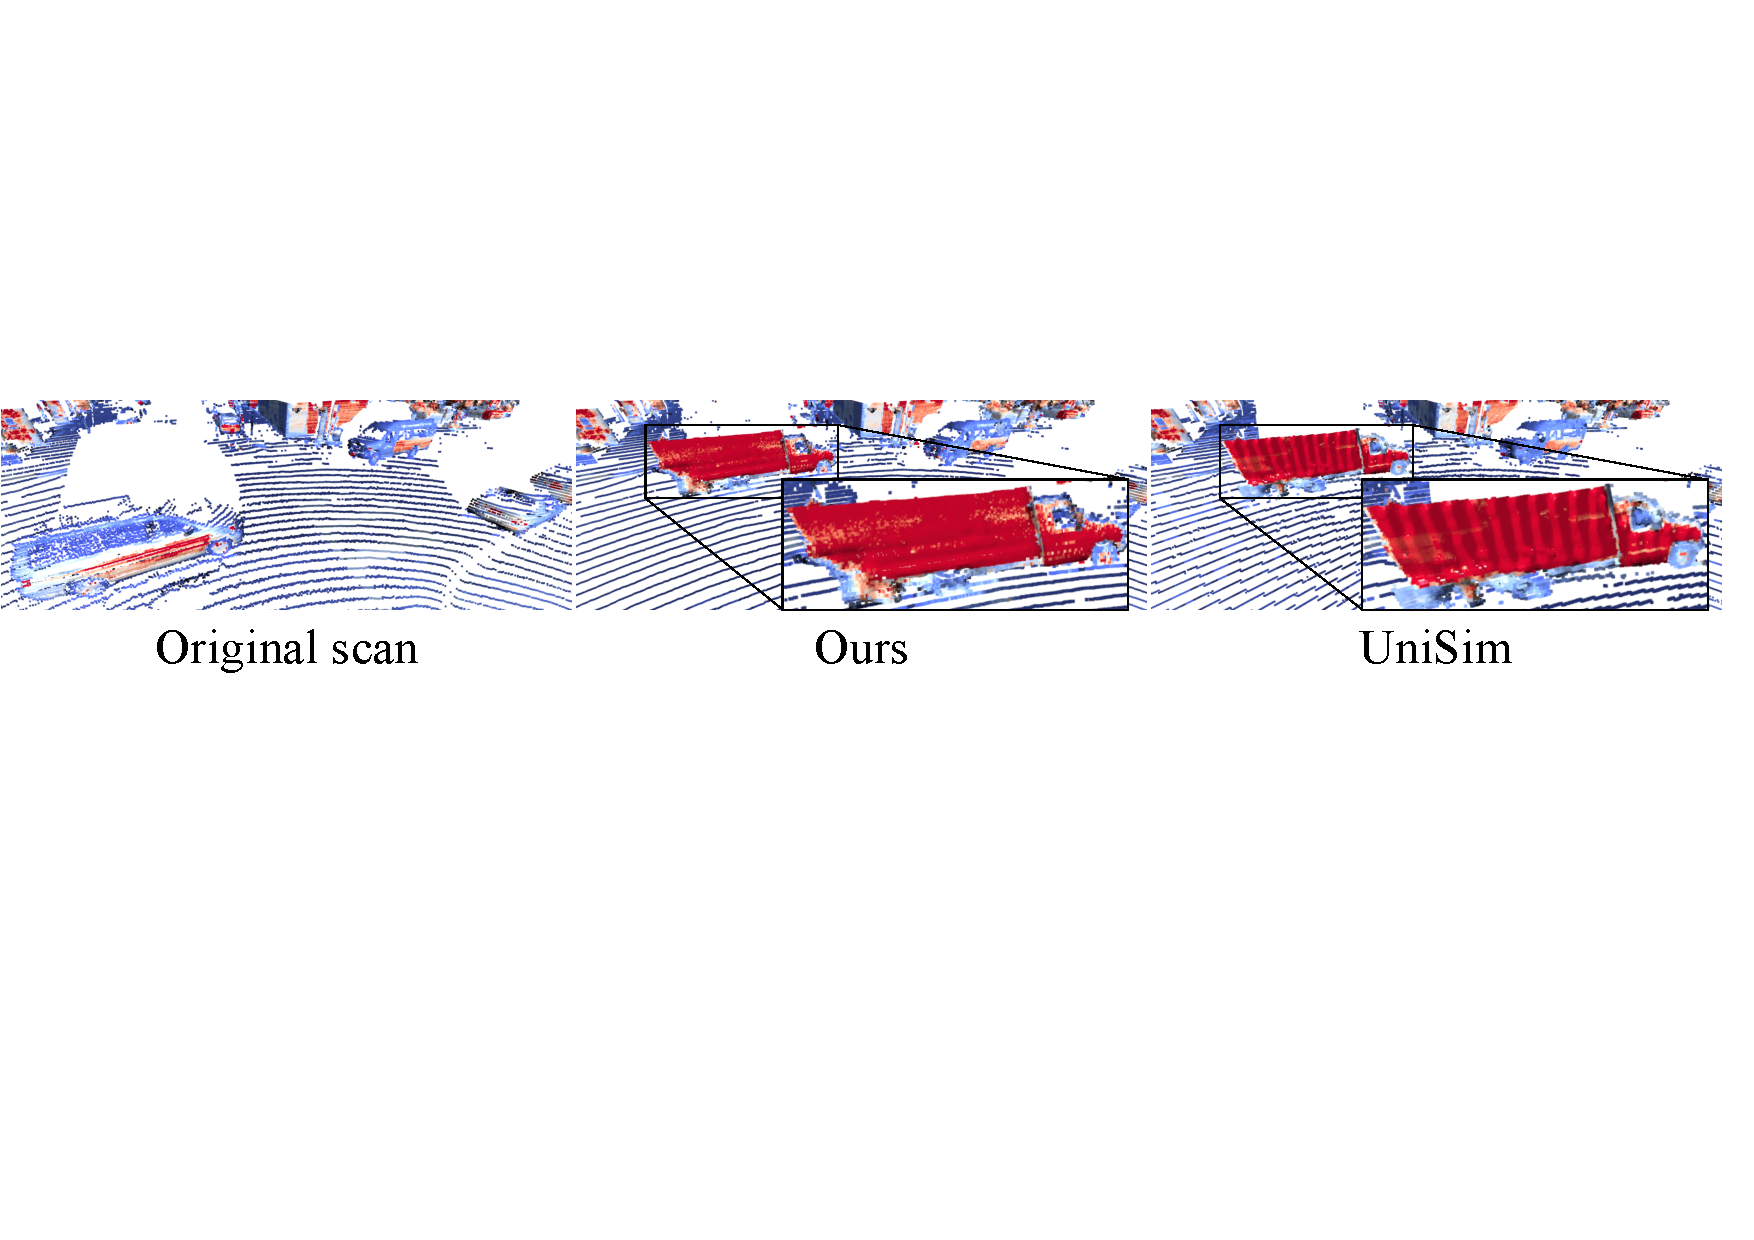
\includegraphics[width=1.0\linewidth]{Figures/vehicle_insertion.pdf}
    
    \caption{
    Qualitative results of object removal and insertion. \dynfl seamlessly inserts the neural asset (truck) into a new scene attributed to our superior compositional rendering scheme. In contrast, UniSim~\cite{yang2023unisim} struggles to accurately model geometry.
    }
    \label{fig:vehicle_insertion}
\end{figure}
\paragraph{Insert object from one scene into another}
Our explicit neural scene de-composition and flexible composition technique enable seamless insertion and removal of neural assets across scenes. As demonstrated in~\cref{fig:vehicle_insertion}, we are able to replace a car from one scene with a truck from another scene, achieving accurate reconstruction of both geometry and intensity. In contrast, UniSim~\cite{yang2023unisim} struggles to preserve high quality geometry. This highlights the significant potential of our approach in generating diverse and realistic LiDAR scans for autonomous driving scenarios.

\begin{figure}[t]
    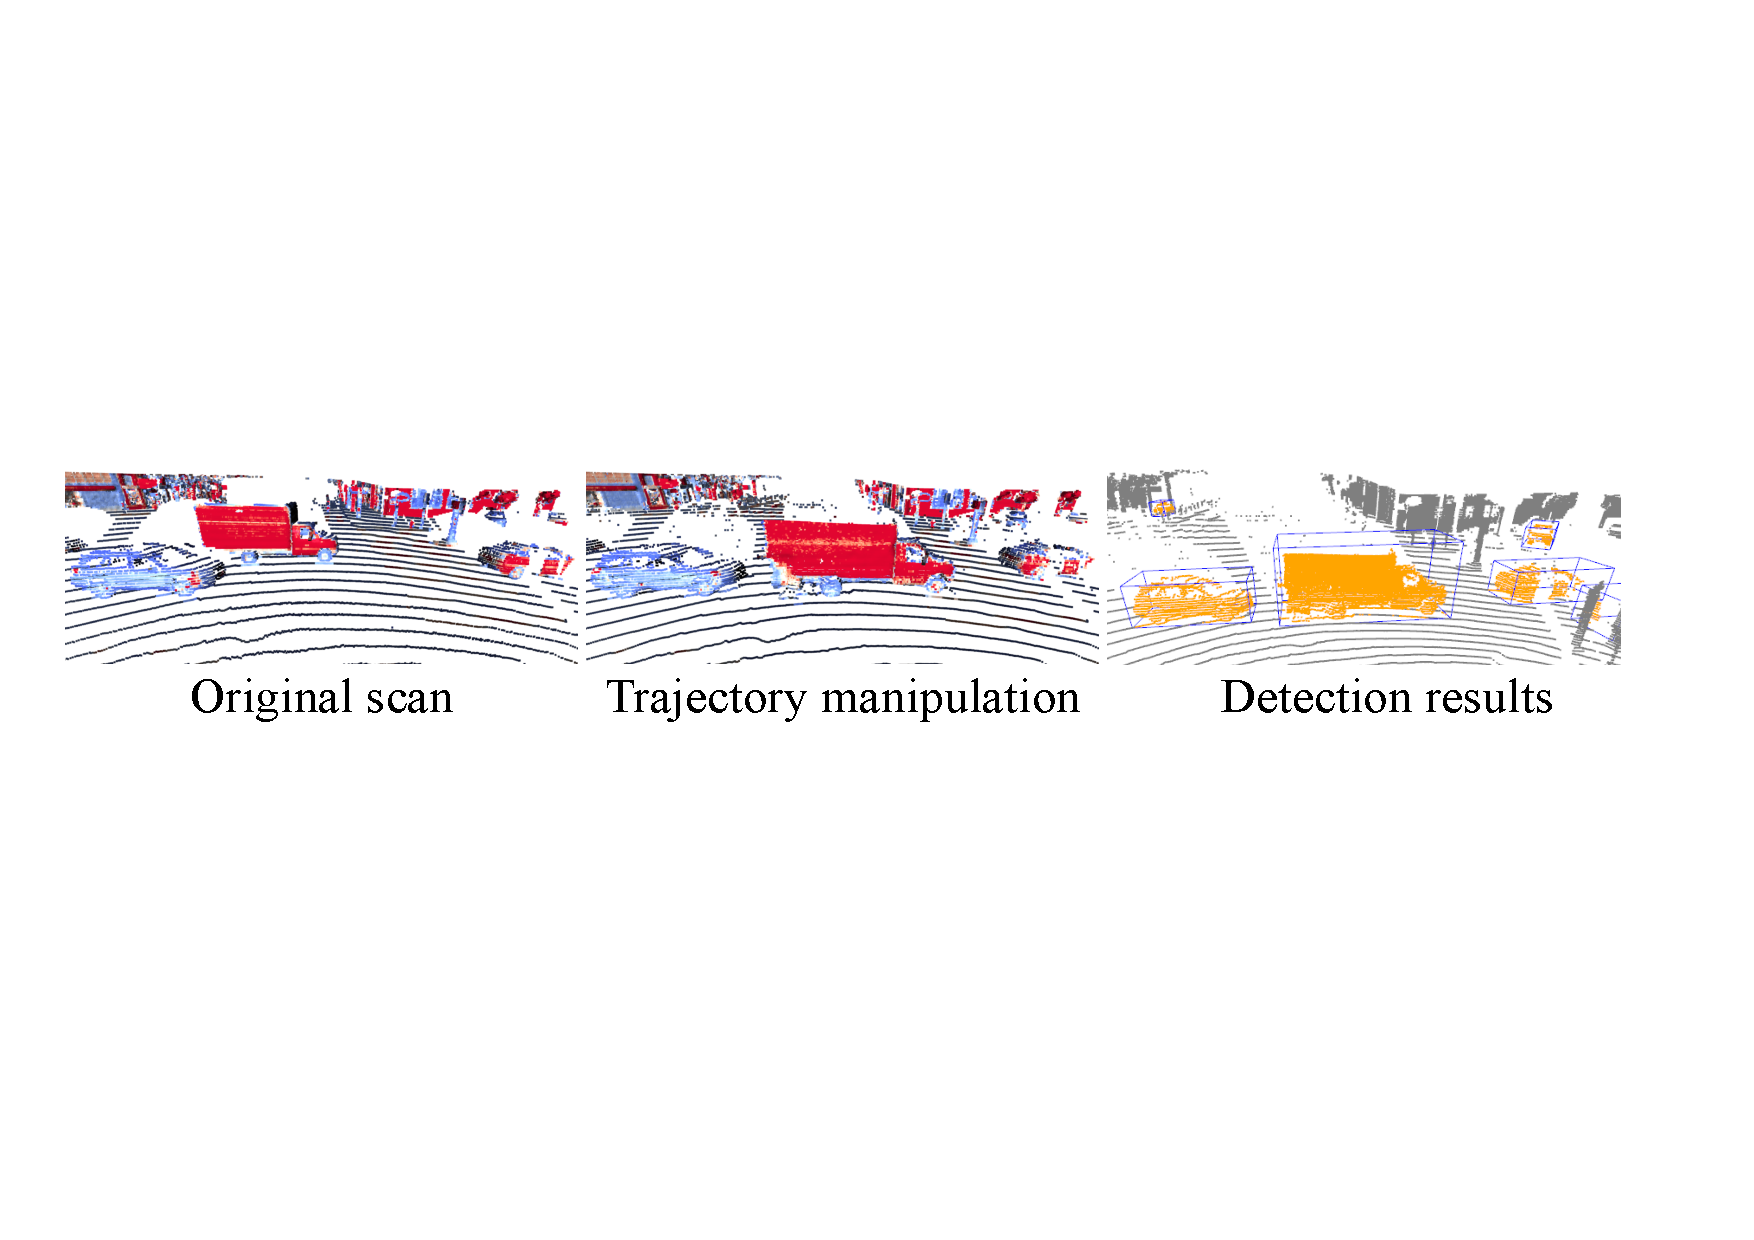
\includegraphics[width=1.0\columnwidth]{Figures/trajectory_manipulation.pdf}
    
    \caption{Qualitative results of object trajectory manipulation. The truck can be successfully detected after manipulation, indicating high-realism LiDAR re-simulation achieved by \dynfl.}
    \label{fig:traj}
    
\end{figure}
\paragraph{Manipulate the trajectory of dynamic objects}
\dynfl also facilitates the manipulation of moving objects' trajectories by simply adjusting their relative poses to the canonical bounding box. Representative results are shown in ~\cref{fig:traj}. The high realism of our re-simulation is also indicated by the successful detection of inserted virtual objects.

\section{Limitations and Future Work}
We present DyNFL, a compositional neural fields approach for LiDAR re-simulation. Our method excels previous art in both static and dynamic scenes, offering powerful scene editing capabilities that open up opportunities for generating diverse and high-quality scenes, to evaluate an autonomy system trained only on real data in closed-loop.

Despite achieving the state-of-the-art performance, there are still limitations we aim to address in future work. Firstly, \dynfl faces challenges in view synthesis of dynamic vehicles from unseen angles. This difficulty arises from the complexity of creating an a-priori model that can accurately complete unseen regions and simulate point cloud noise, ray drops patterns etc. Secondly, our method currently relies on object detection and tracking annotations, and its performance may be compromised when given inaccurate labels. Overcoming this dependency, exploring 4D representations while retaining scene editing flexibility, stands out as a crucial challenge for future research.


\paragraph{Acknowledgements.}
{Or Litany is a Taub fellow and is supported by the Azrieli Foundation Early Career Faculty Fellowship.}

\clearpage
\section{Appendix}
In this supplementary material, we first provide additional information about the datasets for our evaluations and implementation details of our proposed method in~\cref{sec:sup_dataset}. Next, we present more qualitative results in~\cref{sec:sup_visual}. Please also check the supplemental video for more results showcasing our performance. Finally, we provide the complete derivations of the SDF-based volume rendering for active sensor in~\cref{sec:sup_sdf_vol_render}. 

\section{Datasets and implementation details}\label{sec:sup_dataset}
\subsection{Datasets}
\paragraph{\textit{Waymo Dynamic}} For the \textit{Waymo Dynamic} dataset, we take them from 4 scenes of \textit{Waymo Open Dataset}~\cite{sun2020scalability}. There are multiple moving vehicles inside each scene. 50 consecutive frames are taken from each scene for our evaluation. The vehicles are deemed as \textit{dynamic} if the speed is $>1\,$m/s. in any of the 50 frames. The corresponding scene IDs on \textit{Waymo Open Dataset} for our selected scenes are shown as follows:
\begin{table}[!h]
    \setlength{\tabcolsep}{4pt}
    \renewcommand{\arraystretch}{1.2}
	\centering
	\resizebox{0.8\columnwidth}{!}{
    \begin{tabular}{l|c}
    \toprule
    & Scene ID \\
    \midrule
    Scene 1 & 1083056852838271990\_4080\_000\_4100\_000 \\
    Scene 2 & 13271285919570645382\_5320\_000\_5340\_000 \\
    Scene 3 & 10072140764565668044\_4060\_000\_4080\_000 \\
    Scene 4 & 10500357041547037089\_1474\_800\_1494\_800 \\
    \bottomrule
    \end{tabular}
    }
\end{table}

\subsection{Implementation details}
\paragraph{Ours} 
Our model is implemented based on nerfstudio\cite{nerfstudio}. For the static neural field, we sample $N_s=512$ points in total, with $N_u=256$ uniformly sampled points and $N_i=256$ weighted sampled points with 8 upsample steps. In each upsample step, 32 points are sampled based on the weight distribution of the previously sampled points. For each dynamic neural field, we sample $N_s=128$ points in total, with $N_u=64$ uniformly sampled points and $N_i=64$ weighted sampled points with 4 upsample steps. During training, we minimize the loss function using the Adam~\cite{kingma2014adam} optimiser, with an initial learning rate of 0.005. It linearly decays to 0.0005 towards the end of training. For the loss weights, we use $w_{\zeta}=3, w_{e}=50, w_{\text{drop}}=0.15, w_{s}=1$, and  $w_{\text{eik}}=0.3$. The batch size is 4096 and we train the model for 60000 iterations on a single RTX3090 GPU with float32 precision.

\paragraph{LiDARsim} We re-implement the LiDARsim~\cite{manivasagam2020lidarsim} as one of our baselines. 
First, we estimated point-wise normal vectors by considering all points within a 20 cm radius ball within the training set. Following this, we applied voxel down-sampling~\cite{tang2022torchsparse}, employing a 4 cm voxel size to reconstruct individual disk surfels at each point. The surfel orientation is defined based on the estimated normal vector. During inference, we apply the ray-surfel intersections test to determine the intersection points, thus the range and intensity values. We select a fixed surfel radius of 6 cm for the \textit{Waymo} dataset and 12 cm for the \textit{Town} dataset.
To handle dynamic vehicles, we follow LiDARsim~\cite{manivasagam2020lidarsim} by aggregating the LiDAR points for each vehicle from all the training frames and representing them in the \textit{canonical} frame of each vehicle. During inference, we transform all the aggregated vehicle points from their \textit{canonical} frames to the world frame and run ray-surfel intersection.

\paragraph{UniSim} 
We re-implement UniSim's~\cite{yang2023unisim} rendering process for LiDAR measurements by replacing our ray-drop test-based neural fields composition method with its joint rendering method. For every ray $\mathbf{r} (\mathbf{o},\mathbf{d})$, we begin by conducting an intersection test with all dynamic bounding boxes in the scene to identify the near and far limits. We then uniformly sample 512 points along each ray, assigning each point to either a dynamic neural field, if it falls within a dynamic bounding box, or to the static neural field otherwise. After sampling, we query the SDF and intensity values from the relevant neural fields. Finally, using the SDF-based volume rendering formula in Eq.~\ref{eq:depth_render} for active sensors, we calculate the weights and perform the rendering. Note that we use the same neural field architecture as in our method.
\begin{figure*}[t!]
  \centering
   \includegraphics[width=1\textwidth]{Figures_sup/4_scenes_sup.pdf}
   \caption{Visualization of 4 selected scenes from \textit{Waymo Dynamic} dataset. For each scene, we aggregate 50 frames. In the first row, points are color-coded by the intensity values(0 ~\bwrDyNFL~ 0.25). In the second row, dynamic vehicles are painted as \textcolor{yellow}{yellow}.}
   \label{fig:4_scenes_supp}
\end{figure*}

\begin{figure*}[t!]
  \centering
   \includegraphics[width=1\textwidth]{Figures_sup/supp_scene_edit.pdf}
   \caption{Visualization of scene editing capabilities. We showcase 3 kinds of scene editing capabilities including vehicle removal(left), trajectory manipulation(middle) and vehicle insertion(right). The first row represents the original scenes, the second row demonstrates the scenes after editing. All points are color-coded by the intensity values(0 ~\bwrDyNFL~ 0.25).}
   \label{fig:scene_editing_supp}
\end{figure*}

\section{More qualitative results}\label{sec:sup_visual}
In this section, we provide more qualitative results. In \cref{fig:4_scenes_supp}, we showcase the 4 scenes from \textit{Waymo dynamic} dataset. We show additional scene editing results in~\cref{fig:scene_editing_supp}. Please check the supplementary videos for more qualitative results.

\clearpage
\clearpage
\section{SDF-based volume rendering for active sensor}\label{sec:sup_sdf_vol_render}
In this section, we start by introducing the preliminary of NeRF~\cite{mildenhall2020nerf} following terminology as described in~\cite{tagliasacchi2022volume}. Then we provide the full derivation of the SDF-based volume rendering for active sensor. 

\subsection{Preliminary}\label{sec:supp_pre}
\paragraph{Density}
For a ray emitted from the origin $\origin \in \real^3$ towards direction $\dir \in \real^3$, the \textit{density} $\density_\zeta$ at range $\zeta$ indicates the likelihood of light interacting with particles at that point $\ray_\zeta = \origin + \zeta \dir$. This interaction can include absorption or scattering of light. In passive sensing, density $\density$ is a critical factor in determining how much light from the scene's illumination is likely to reach the sensor after passing through the medium.
\paragraph{Transmittance} quantifies the likelihood of light traveling through a given portion of the medium without being scattered or absorbed. Density is closely tied to the transmittance function $\transmittance(\zeta)$, which indicates the probability of a ray traveling over the interval $[0, \zeta)$ without hitting any particles. Then the probability $\transmittance(\zeta {+} d\zeta)$ of \emph{not} hitting a particle when taking a differential step $d\zeta$ is equal to $\transmittance(\zeta)$, the likelihood of the ray reaching $\zeta$, times $(1 - d\zeta \cdot \density(\zeta))$, the probability of not hitting anything during the step:
% 
\begin{align}
\transmittance(\zeta+d\zeta) =& \transmittance(\zeta) \cdot (1 - d\zeta \cdot \density(\zeta))
\\
\frac{\transmittance(\zeta+d\zeta) - \transmittance(\zeta)}{d\zeta} \equiv& \transmittance'(\zeta) = -\transmittance(\zeta) \cdot \sigma(\zeta) 
\label{eq:derivative}
\end{align}
% 
We solve the differential equation as follows:
%
\begin{align}
\transmittance'(\zeta) &= -\transmittance(\zeta) \cdot \density(\zeta) \\
\frac{\transmittance'(\zeta)}{\transmittance(\zeta)} &= -\density(\zeta) \\
\int_a^b \frac{\transmittance'(\zeta)}{\transmittance(\zeta)} \; d\zeta &= -\int_a^b \density(\zeta) \; d\zeta \\
\left. \log \transmittance(\zeta) \right|_a^b &= -\int_a^b \density(\zeta) \; d\zeta \\
\transmittance(a \rightarrow b) \equiv \frac{\transmittance(b)}{\transmittance(a)} &= \exponential{-\int_a^b \density(\zeta) \; d\zeta}   
\end{align}
% 
Hence, for a ray segment between $\zeta_0$ and $\zeta$, transmittance is given by:

\begin{equation}
\transmittance_{\zeta_0 \rightarrow \zeta} \equiv \frac{\transmittance_{\zeta}}{\transmittance_{\zeta_0}} = exp({-\int_{\zeta_0}^\zeta \density_t dt})\;,
\label{eq:trans_ab}
\end{equation}
which leads to following factorization of the transmittance:
\begin{equation}
\transmittance_{\zeta} = \transmittance_{0 \rightarrow \zeta_0} \cdot \transmittance_{\zeta_0 \rightarrow \zeta}\;.
\label{eq:factor}
\end{equation}

\paragraph{Opacity}Opacity is the complement of transmittance and represents the fraction of light that is either absorbed or scattered in the medium. In a homogeneous medium with constant density $\density$  the opacity for a segment $[\zeta_j, \zeta_{j+1}]$ of length $\Delta \zeta$ is given by $\opacity_{\zeta_j} = 1 - exp(-\density \cdot \Delta \zeta)$
\subsection{SDF-based volume rendering for active sensor}\label{sec:sdf_active}
NeuS\cite{wang2021neus} derives the opaque density based on the SDF which is:
\begin{equation}
\begin{split}
\density_{\zeta_i} =&  \max\left(\frac{-\frac{d\Phi_s}{d\zeta_i}(f(\zeta_i))}{\Phi_s(f(\zeta_i))},0\right)\\
                  =& \max\left(\frac{-(\nabla f(\zeta_i)\cdot \mathbf{v})\phi_s(f(\zeta_i))}{\Phi_s(f(\zeta_i))}, 0\right)
\end{split}
\label{eq:sigmoid_density}
\end{equation}
where $\Phi_s$ represents the Sigmoid function, $f$ is the SDF function that maps a range $\zeta$ to the SDF value of the point position $\origin + \dir * \zeta$. Note that the integral term is computed by
\begin{equation}
\int \frac{-(\nabla f(\zeta)\cdot \mathbf{v})\phi_s(f(\zeta))}{\Phi_s(f(\zeta))}d\zeta = -\ln(\Phi_s(f(\zeta))) + C,
\label{eq:intergration_density}
\end{equation}
% We can then calculate the accumulated transmittance from \ref{eq:trans_ab} using \ref{eq:intergration_density}:
% % 
% \begin{align}
% \transmittance_\zeta = \transmittance(0 \rightarrow \zeta) 
% % &= \prod_{k=1}^{n-1} \transmittance(t_k \rightarrow t_{k+1}) 
% &= \exponential{- \int_{0}^{\zeta} \density(t) \; dt} 
% = \Phi_s(f(\zeta))
% \label{eq:trans_const}
% \end{align}
We extend the density-based volume rendering for active sensor to SDF-based. Starting from the passive SDF-based volume rendering \cite{wang2021neus}, We substitute the density $\tilde{\density}$ with opaque density in \ref{eq:sigmoid_density}
and evaluate the radiant power integrated from ray segment [a,b] with constant reflectivity $\reflectivity_a$.

Consider the case where $-(\nabla f(\zeta)\cdot \mathbf{v})>0$ within the ray segment $[a,b]$, we have
\begin{align}
P(a \rightarrow b)
&= \int_a^b \transmittance^2(a\rightarrow t) \cdot \tilde{\density}_t \cdot \reflectivity(t)  \; dt
\\
&= \reflectivity_a \int_a^b \transmittance^2(a\rightarrow t) \cdot \tilde{\density}_t \; dt
\\
&= \reflectivity_a \int_a^b \exponential{-\int_a^t 2\tilde{\density}(u) \; du} \cdot \tilde{\density}_t \; dt
\\
&= \reflectivity_a \int_a^b \exponential{-2\int_a^t \tilde{\density}(u) \; du} \cdot \tilde{\density}_t \; dt
\\
&= \reflectivity_a \int_a^b \exponential{\left. 2\ln(\Phi_s(f(u)))\right|_a^t} \cdot \tilde{\density}_t \; dt
\\
% &= \reflectivity_a \int_a^b \exponential{2\ln(\Phi_s(f(t))) - 2\ln(\Phi_s(f(a)))} \cdot \tilde{\density}_t \; dt \\
&= \reflectivity_a \int_a^b \exponential{2\ln(\Omega_t) - 2\ln(\Omega_a)} \cdot \tilde{\density}_t \; dt 
\\
&= \reflectivity_a \int_a^b \frac{{\Omega_t}^2}{{\Omega_a}^2} \cdot \tilde{\density}_t \; dt ~~~~\text{\textbf{let} $\Omega_x = \Phi_s(f(x))$}
\\
&= \frac{\reflectivity_a}{{\Omega_a}^2} \int_a^b {\Omega_t}^2 \cdot \tilde{\density}_t \; dt 
\\
&= \frac{\reflectivity_a}{{\Omega_a}^2} \int_a^b -\frac{d\Phi_s}{dt}(f(t)) \cdot \Phi_s(f(t)) \; dt 
% \quad \text{$\tilde{\density}_t = \frac{-\frac{d\Phi_s}{d t}(f(t))}{\Phi_s(f(t))}$}
\\
&= \frac{\reflectivity_a}{{\Omega_a}^2} ( \left. -\frac{1}{2}{\Phi_s(f(t))}^2 \right|_a^b) \\
&= \frac{\reflectivity_a}{{\Omega_a}^2} (\frac{1}{2}{\Phi_s(f(a))}^2 -\frac{1}{2}{\Phi_s(f(b))}^2 )\\
&= \frac{{\Phi_s(f(a))}^2 -{\Phi_s(f(b))}^2}{{2\Phi_s(f(a))}^2} \cdot \reflectivity_a 
% \quad \text{$T_a$ = $\Phi_s(f(a))$}
\label{eq:homogeneous}
\end{align}
%\cref{eq:trans_const}

Consider the case where $-(\nabla f(\zeta)\cdot \mathbf{v})<0$ within the ray segment $[a,b]$, we have
\begin{align}
P(a \rightarrow b)
&= \int_a^b \transmittance^2(a\rightarrow t) \cdot \tilde{\density}_t \cdot \reflectivity(t)  \; dt
\\
&= \int_a^b \transmittance^2(a\rightarrow t) \cdot 0 \cdot \reflectivity(t)  \; dt
\\
&= 0
\end{align}
Hence we conclude 
\begin{align}
P(a \rightarrow b)
&= \max\left(\frac{{\Phi_s(f(a))}^2 -{\Phi_s(f(b))}^2}{{2\Phi_s(f(a))}^2},0\right) \cdot \reflectivity_a 
\end{align}

\paragraph{Volume rendering of piecewise constant data}
Combining the above, we can evaluate the volume rendering integral through a medium with piecewise constant reflectivity:
% 
\begin{align}
P(\zeta_{N+1}) &= \sum_{n=1}^N \int_{\zeta_n}^{\zeta_{n+1}} \transmittance^2(\zeta) \cdot \tilde{\density}_{\zeta} \cdot \reflectivity_{\zeta_n} \; d\zeta
\\
&= \sum_{n=1}^N \int_{\zeta_n}^{\zeta_{n+1}} \transmittance^2_{\zeta_n} \cdot \transmittance^2(\zeta_n \shortto \zeta) \cdot \tilde{\density}_{\zeta} \cdot \reflectivity_{\zeta_n} \; d\zeta 
% &&\text{from \ref{eq:factor}}
\\
&= \sum_{n=1}^N \transmittance^2_{\zeta_n}  \int_{\zeta_n}^{\zeta_{n+1}} \transmittance^2(\zeta_n \rightarrow \zeta) \cdot \tilde{\density}_{\zeta} \cdot \reflectivity_{\zeta_n} \; d\zeta \\
% &&\text{constant}
% \\
&=\sum_{n=1}^N \transmittance^2_{\zeta_n} P(\zeta_n \rightarrow \zeta_{n+1})
\\
&= \sum_{n=1}^N \transmittance^2_{\zeta_n} \cdot \tilde{\weight}_{\zeta_n} \cdot \reflectivity_{\zeta_n},
% &&\text{from \ref{eq:homogeneous}}
\end{align}

where 
\begin{align}
\tilde{\weight}_{\zeta_n} \equiv \max\left(\frac{{\Phi_s(f(\zeta_n)}^2 -{\Phi_s(f(\zeta_{n+1}))}^2}{{2\Phi_s(f(\zeta_n))}^2},0\right)
\end{align}
% 
% This leads to the volume rendering equations from NeRF~\cite[Eq.3]{mildenhall2020nerf}:
% % 
% \begin{align}
% P(\zeta_{N+1}) = \sum_{n=1}^N \transmittance^2_{\zeta_n} \cdot \frac{{\Phi_s(f(\zeta_n))}^2 -{\Phi_s(f(\zeta_{n+1}))}^2}{{2\Phi_s(f(\zeta_n))}^2} \cdot \reflectivity_{\zeta_n}
% \label{eq:final_radiant}
% \end{align}
% % 
% Since the opacity is always greater than 0, we can express the opacity as
% \begin{equation}
%     \tilde{\weight}_{\zeta_n} \equiv max(\frac{{\Phi_s(f(\zeta_n))}^2 -{\Phi_s(f(\zeta_{n+1}))}^2}{{2\Phi_s(f(\zeta_n))}^2}, 0)
%     \label{eq:opacity}
% \end{equation}

The discrete accumulated transmittance $\transmittance$ can be calculated as follows:

Consider the case where $-(\nabla f(\zeta)\cdot \mathbf{v}) > 0$ in $[\zeta_n, \zeta_{n+1}]$: 
%
\begin{align}
\transmittance_{\zeta_n} 
&=\prod_{i=1}^{n-1}(\exp(-\int_{\zeta_n}^{\zeta_{n+1}}\tilde{\density}_\zeta \; d\zeta) \\
&= \prod_{i=1}^{n-1}(\frac{\Phi_s(f(\zeta_{n+1}))}{\Phi_s(f(\zeta_n))})\\
\transmittance^2_{\zeta_n}
&= \prod_{i=1}^{n-1}(\frac{{\Phi_s(f(\zeta_{n+1}))}^2}{{\Phi_s(f(\zeta_n))}^2})\\
&= \prod_{i=1}^{n-1}(1-2\tilde{\weight}_{\zeta_n})
\label{eq:dicrete_transmittance}
\end{align}

Consider the case where $-(\nabla f(\zeta)\cdot \mathbf{v}) < 0$ in $[\zeta_n, \zeta_{n+1}]$: 
\begin{align}
\transmittance_{\zeta_n} 
&=\prod_{i=1}^{n-1}(\exp(-\int_{\zeta_n}^{\zeta_{n+1}}\tilde{\density}_\zeta \; d\zeta) = \prod_{i=1}^{n-1}(1)
\\
\transmittance^2_{\zeta_n} &= \prod_{i=1}^{n-1}(1^2) = \prod_{i=1}^{n-1}(1-2\tilde{\weight}_{\zeta_n})
\end{align}
In conclusion, the radiant power can be reformulated as:

\begin{align}
P(\zeta_{N+1}) = \sum_{n=1}^N \transmittance^2_{\zeta_n} \cdot \tilde{\weight}_{\zeta_n} \cdot \reflectivity_{\zeta_n}
\label{eq:final_radiant2}
\end{align}
where $\transmittance^2_{\zeta_n} = \prod_{i=1}^{n-1}(1-2\tilde{\weight}_{\zeta_i})$


\paragraph{Depth volume rendering of piecewise constant data}

Note that $\tilde{\weight}_{\zeta_n} \in [0, 0.5], \transmittance^2_{\zeta_n} \in [0,1], \sum_{n=1}^N \transmittance^2_{\zeta_n} \cdot \tilde{\weight}_{\zeta_n} = 0.5$, for depth volumetric rendering, we have 
\begin{align}
    \zeta = \sum_{n=1}^N 2 \cdot \transmittance^2_{\zeta_n} \cdot \tilde{\weight}_{\zeta_n} \cdot \zeta_n
    =\sum_{n=1}^N w_n \cdot \zeta_n
    \label{eq:depth_render}
\end{align}
where $w_n = 2\tilde{\weight}_{\zeta_n} \cdot \prod_{i=1}^{n-1}(1-2\tilde{\weight}_{\zeta_i})$

\renewcommand{\subdir}{tex/CVPR2024_Dynamic_NFL}
\chapter[Dynamic LiDAR Re-simulation using Compositional Neural Fields]{Dynamic LiDAR Re-simulation using Compositional Neural Fields}
\label{chap:cvpr24}

Hanfeng Wu, Xingxing Zuo, Stefan Leutenegger, Or Litany, Konrad Schindler, Shengyu Huang \\
\textbf{IEEE/CVF Conference on Computer Vision and Pattern Recognition, 2024}\\
\\
(Author version; for typeset version please refer to the original conference paper.)\\

\providecommand{\subdir}{.}
\graphicspath{{\subdir/}}

\section*{Abstract}
We present Neural Fields for LiDAR (NFL), a method to optimise a neural field scene representation from LiDAR measurements, with the goal of synthesizing realistic LiDAR scans from novel viewpoints. 
NFL combines the rendering power of neural fields with a detailed, physically motivated model of the LiDAR sensing process, thus enabling it to accurately reproduce key sensor behaviors like beam divergence, secondary returns, and ray dropping.
We evaluate NFL on synthetic and real LiDAR scans and show that it outperforms explicit reconstruct-then-simulate methods as well as other NeRF-style methods on LiDAR novel view synthesis task. Moreover, we show that the improved realism of the synthesized views narrows the domain gap to real scans and translates to better registration and semantic segmentation performance. Project page: \url{https://research.nvidia.com/labs/toronto-ai/nfl}.
\newpage
\section{Introduction}
\begin{figure*}[t]
    \centering
        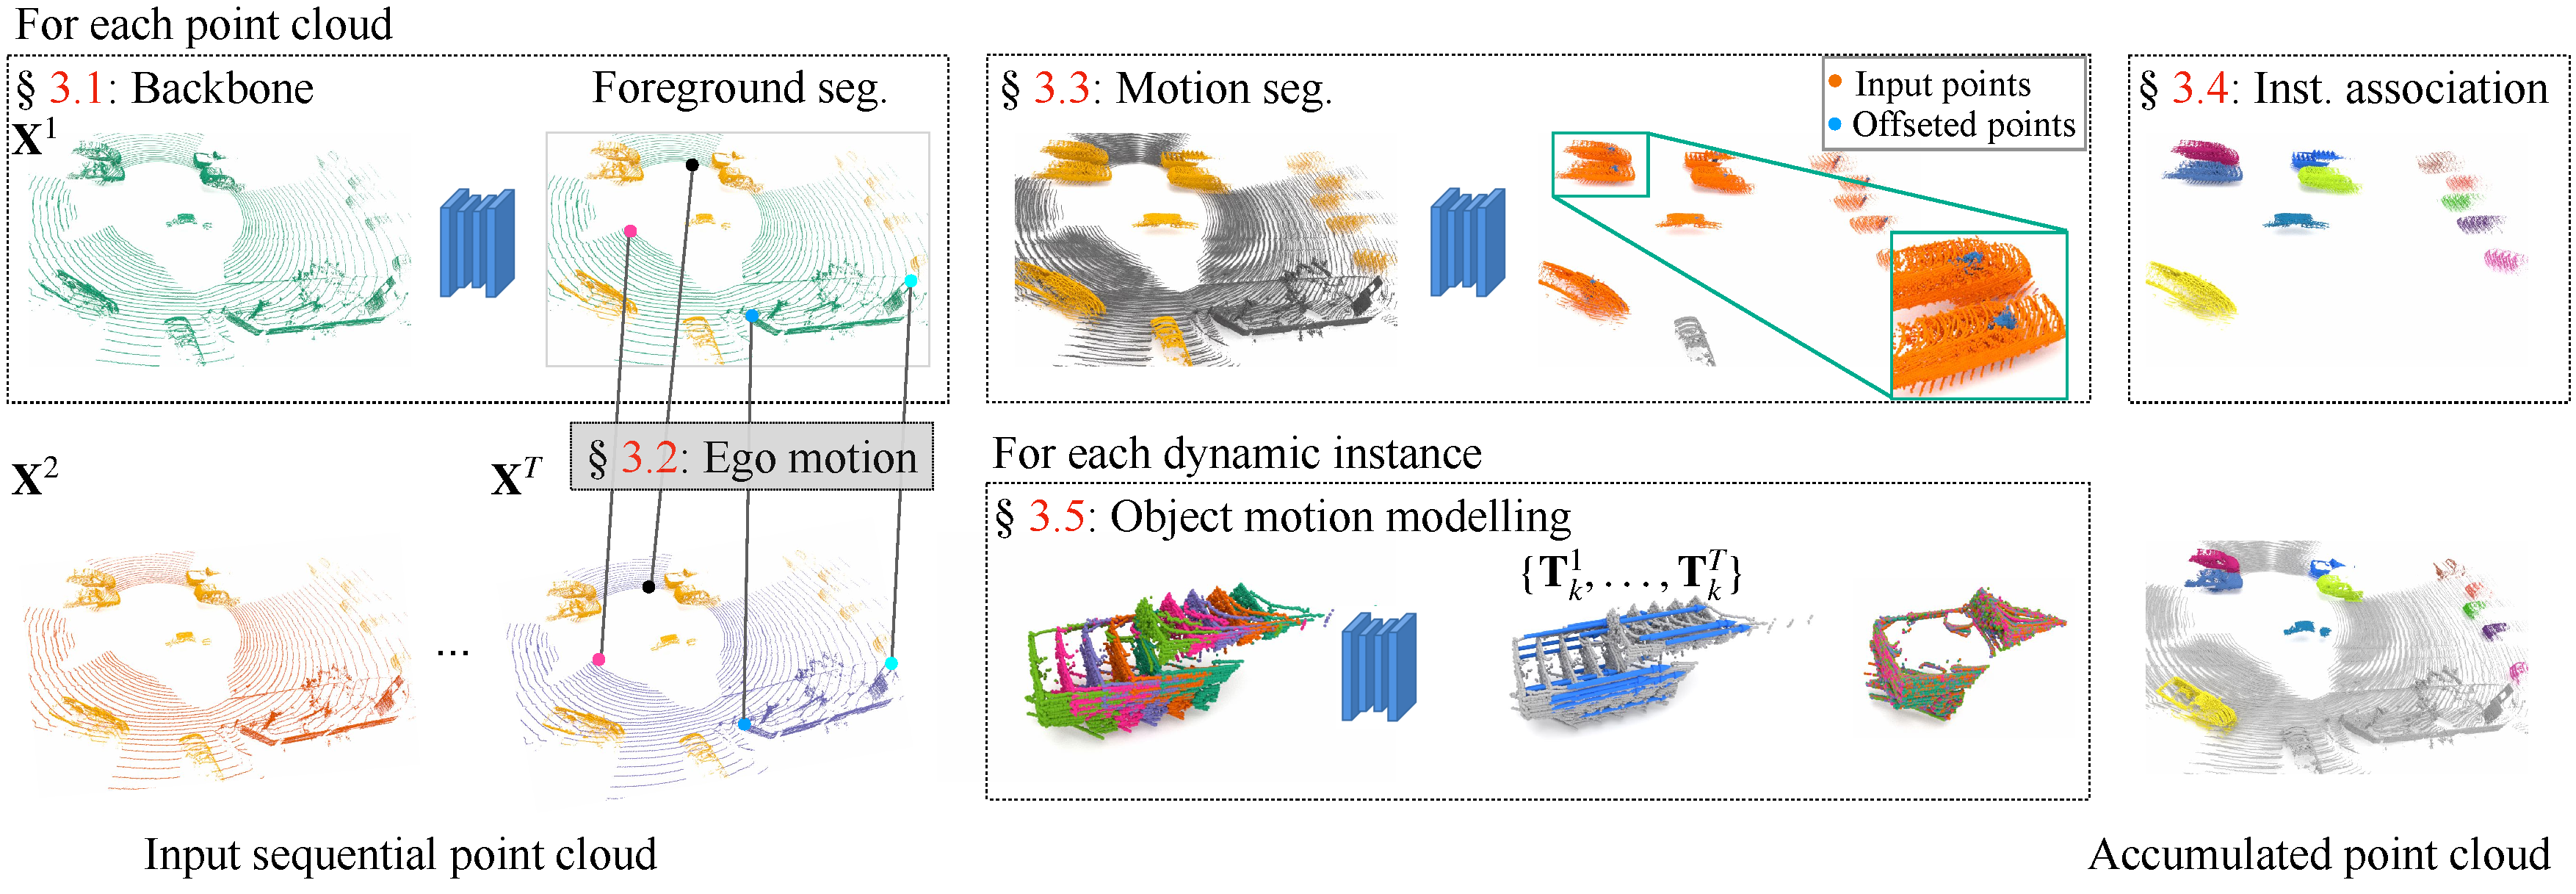
\includegraphics[width=1.0\textwidth]{Figures/overview.pdf}
        \caption{
        Overview of \dynfl. Our method takes LiDAR scans and tracked bounding boxes of dynamic vehicles as input. \dynfl first decomposes the scene into a static background and $N$ dynamic vehicles, each modelled using a dedicated neural field. These neural fields are then composed to re-simulate LiDAR scans in dynamic scenes. Our composition technique supports various scene edits, including altering object trajectories, removing and adding reconstructed neural assets between scenes.
    }
    \label{fig:main}
\end{figure*}

We introduce a neural representation for the purpose of reconstructing and manipulating LiDAR scans of dynamic driving scenes. 
Counterfactual re-simulation is an emerging application in the realm of autonomous driving, offering a unique approach to examining "what if" scenarios. This method involves creating a reconstruction of a real-world event, termed as \textit{digital twin} and then applying various modifications to it. These could include altering the environmental conditions, changing the action of some agent, or introducing additional scene elements. Analyzing the outcomes of these edited scenarios provides insights into the functioning of the perception system, moreover they can be used to obtain training data for rare situations.

The essence of counterfactual re-simulation is the capability to authentically recreate variations of the original, factual observation. We address this challenge in the context of LiDAR on autonomous vehicles (AV). Existing approaches to LiDAR re-simulation have important limitations. Conventional simulators such as CARLA~\cite{dosovitskiy2017carla} and NVIDIA DRIVE Sim are capable of modeling LiDAR sensors. However, their reliance on manually designed 3D simulation assets requires significant human effort. LiDARsim~\cite{manivasagam2020lidarsim} aims to remedy this by reconstructing vehicles and scenes from real measurements. While producing encouraging results, its two-stage LiDAR modeling lacks realism, particularly in terms of physical effects like multi-returns and reflected intensity, which were shown 
 to matter for downstream processing~\cite{guillard2022learning}. Following NeRF's~\cite{mildenhall2020nerf} success in camera view synthesis, some works have applied neural fields for LiDAR modeling~\cite{Huang2023nfl, tao2023lidar, zhang2023nerf}. In particular, Neural LiDAR Fields (NFL)\cite{Huang2023nfl} developed a physically inspired LiDAR volumetric rendering scheme that accounts for two-way transmittance and beam width, allowing faithful recovery of secondary returns, intensity, and ray drops. These models are, however, limited to static scenes that do not change while multiple input views are scanned, and are thus of limited use for re-simulation in the presence of moving traffic. Recently, UniSim~\cite{yang2023unisim} followed Neural Scene Graph~\cite{Ost_2021_CVPR} in modeling road scenes as sets of movable NeRF instances on top of a static background. UniSim introduced a unified synthesis approach for camera and LiDAR sensors, but ignored physical sensor properties like two-way transmittance and beam width~\cite{Huang2023nfl}.

We present \dynfl, a novel approach for re-simulating LiDAR views of driving scenarios. Our method builds upon a neural SDF that enables an accurate representation of scene geometry, while at the same time enforcing physical accuracy by modeling two-way transmittance, like NFL~\cite{Huang2023nfl}. 
% Our method builds upon UniSim's SDF representation and scene decomposition, but enhances the physical accuracy by incorporating two-way transmittance modeling, as introduced in NFL.
%
Our primary contribution is a method for compositing neural fields that accurately integrates LiDAR measurements from individual fields representing different scene assets. With the help of a ray drop test, we effectively manage occlusions and transparent surfaces. This not only ensures physical accuracy, but also facilitates the inclusion of assets reconstructed from a variety of static and dynamic scenes, thereby enhancing control over the simulated content. Our method bridges the gap between the physical fidelity of the re-simulation and flexible editing of dynamic scenes.
%
We validate \dynfl with both synthetic and real-world data, focusing on three key areas: \textit{(i)} high-quality view synthesis, \textit{(ii)} perceptual fidelity, and \textit{(iii)} asset manipulation. We find that our approach outperforms baseline models \wrt both range and intensity. Its synthetic outputs also show higher agreement with real scans in terms of object detection and segmentation. Furthermore, \dynfl enables not only removal, duplication and repositioning of assets within the same scene, but also the inclusion of assets reconstructed in other scenes, paving the way for new applications.


% In the rapidly evolving field of computer vision, novel view synthesis has become a groundbreaking technique, especially in the realm of image-based rendering. Pioneered by technologies like NeRF~\cite{mildenhall2020nerf}, it allows for the creation of photo-realistic views from a given set of data. However, the application of these principles to LiDAR data, which inherently deals with point clouds, introduces a complex set of challenges and opportunities that are distinct from traditional image-based approaches.

% Historically, methods like LiDARsim~\cite{manivasagam2020lidarsim} have paved the way for such advancements, yet they exhibit limitations. Specifically, LiDARsim operates by first extracting an explicit scene representation and then performing ray-surfel casting to synthesize LiDAR scans. This approach, while innovative, is susceptible to inaccuracies due to point cloud noise and typically results in lower reconstruction quality. This limitation leads to a significant domain gap when compared to ground truth LiDAR scans. Our previous work, Neural Lidar Fields (NFL)~\cite{Huang2023nfl}, marked a substantial improvement in modeling LiDAR scenes with neural fields and incorporating the physical characteristics of LiDAR beams. Despite its state-of-the-art performance in geometry reconstruction, NFL was limited to static scenes and did not address the complexities of dynamic environments.

% In dynamic scenarios, particularly in automotive or robotics contexts, capturing the constant motion of elements like vehicles and pedestrians is crucial. Our work seeks to bridge this gap by extending the principles of NFL to dynamic settings. Prior approaches that tackle the dynamic scenes, such as LiDARsim~\cite{manivasagam2020lidarsim}, have adopted a reconstruct-then-simulate process, resulting in inferior geometric fidelity. Meanwhile, other neural-fields-based explorations like Neural Scene Graph~\cite{Ost_2021_CVPR} and UniSim~\cite{yang2023unisim} focus on image-based rendering or sensor fusion, neglecting LiDAR-specific attributes.

% In this context, our work contributes in several ways:
% \textbf{1.)} Improved Geometry Quality: We adopt a Signed Distance Function (SDF)-based volume rendering approach, specifically tailored to the active sensor characteristics of LiDAR beam. This method acknowledges and leverages the intricacies of how LiDAR sensors capture data, resulting in reconstructions of higher fidelity and geometric accuracy.
% \textbf{2.)} Innovative Neural Fields Composition: Our methodology introduces a novel technique for the composition of multiple neural fields. This approach significantly enhances the rendering process, allowing for seamless integration and higher-quality synthesis of dynamic views.

% Our paper delves into the technicalities of Dynamic Neural LiDAR Fields, elaborating on the methods and innovations that enable the synthesis of dynamic views from LiDAR data. We present extensive experimental results that showcase the effectiveness of our approach in dynamic environments, illustrating how our contributions extend the applicability of neural LiDAR fields. Through this work, we provide a valuable resource for researchers in computer vision, contributing to the broader discourse on LiDAR novel view synthesis for dynamic scenes.


\section{Related work}
\paragraph{Neural radiance fields and volume rendering}
Neural Radiance Fields (NeRF)~\cite{mildenhall2020nerf} have demonstrated remarkable success in novel-view image synthesis through neural volume rendering. These fields are characterized by the weights of Multilayer Perceptrons (MLPs), which enable the retrieval of volume density and RGB colors at any specified point within the field for image compositing via volume rendering. Several studies~\cite{barron2021mip,barron2022mip,verbin2022ref,chen2022tensorf,fridovich2022plenoxels} have subsequently advanced NeRF's rendering quality by addressing challenges such as reducing aliasing artifacts~\cite{barron2021mip}, scaling to unbound large-scale scenarios~\cite{barron2022mip}, and capturing specular reflections on glossy surfaces~\cite{verbin2022ref}.
Certain works~\cite{chen2022tensorf,fridovich2022plenoxels,mueller2022instant,kerbl20233d} have explored more effective representations of radiance fields. TensorsRF~\cite{chen2022tensorf} employs multiple compact low-rank tensor components, such as vectors and matrices, to represent the radiance field. Plenoxels~\cite{fridovich2022plenoxels} accelerates NeRF training by replacing MLPs with explicit plenoptic elements stored in sparse voxels and factorizing appearance through spherical-harmonic functions.
M\"uller et al.~\cite{mueller2022instant} achieved a substantial acceleration in rendering speed by employing a representation that combines trainable multi-resolution hash encodings (MHE) with shared shallow MLP networks. Kerbel et al.~\cite{kerbl20233d} introduce a novel volume rendering method utilizing 3D Gaussians to represent the radiance field and rendering images based on visibility-aware splatting of 3D Gaussians.


\paragraph{Dynamic neural radiance fields} 
Neural fields \cite{xie2022neural} can be extended to represent dynamic scenes. On top of the \textit{canonical} scene representation, some methods~\cite{pumarola2020d, park2021nerfies, park2021hypernerf,yuan2021star} additionally model the 4D deformation fields. Meanwhile, some other works learn a space-time correlated~\cite{kplanes_2023, li2020neural, attal2023hyperreel, liu2023robust}, or decomposed~\cite{turki2023suds,wu2022d,yang2023emernerf} neural field to encode the 4D scenes, achieving fine-grained reconstruction of the geometry and the appearance.
%
Some other methods decompose the scene into static and dynamic parts, and model each dynamic actor with dedicated neural fields. 
Neural Scene Graph~\cite{Ost_2021_CVPR} and Panoptic Neural Fields~\cite{KunduCVPR2022PNF} treat every dynamic object in the scene as a node, and synthesize photo-realistic RGB images by jointly rendering from both dynamic nodes and static background. UniSim\cite{yang2023unisim} employs neural SDF representation to model dynamic scenes in driving scenarios, and render in a similar way to Neural Scene Graph~\cite{Ost_2021_CVPR}.


\paragraph{Neural surface representation}
A fundamental challenge for NeRF and its variants involves accurately recovering the underlying 3D surface from the implicit radiance field. Surfaces obtained by thresholding on the volume density of NeRF often exhibit noise~\cite{wang2021neus, yariv2021volume}. To address this, implicit surface representations like Occupancy~\cite{niemeyer2020differentiable, oechsle2021unisurf} and signed distance functions (SDF)~\cite{wang2021neus, yariv2021volume, yu2022monosdf, sun2022neural, wang2022hf, zuo2023incremental, li2023neuralangelo, wang2023neus2} in grid maps are commonly integrated into neural volume rendering techniques.

NeuS~\cite{wang2021neus} introduces a neural SDF representation for surface reconstruction, proposing an unbiased weight function for the appearance composition process in volume rendering. Similarly, VolSDF~\cite{yariv2021volume} models scenes with a neural SDF and incorporates the SDF into the volume rendering process, advocating a sampling strategy of the viewing ray to bound opacity approximation error. Neuralangelo~\cite{li2023neuralangelo} improves surface reconstruction using the multi-resolution hash encoding (MHE)~\cite{mueller2022instant} and SDF-based volume rendering~\cite{wang2021neus}. While these methods might deliver satisfying dense surface reconstructions, their training is time-consuming, taking hours for a single scene.
Voxurf~\cite{wu2022voxurf} offers a faster surface reconstruction method through a two-stage training procedure, recovering the coarse shape first and refining details later. Wang et al.~\cite{wang2023neus2} expedites NeuS training to several minutes by predicting SDFs through a pipeline composed of MHE and shallow MLPs.

Many works also incorporate distances measured by LiDAR as auxiliary information to constrain the radiance field. For instance, works~\cite{chang2023neural, wang2023neural} render depth by accumulating volume density and minimizing depth discrepancies between LiDAR and render depth during training. Rematas et al.~\cite{rematas2022urban} enforces empty space between the actual surface and the ray origin.


\paragraph{LiDAR simulation} 
While simulators like CARLA~\cite{dosovitskiy2017carla} and AirSim~\cite{shah2018airsim} can simulate LiDAR data, they suffer from expensive human annotation requirements and a notable sim-to-real gap due to limited rendering quality. Generative model-based methods for LiDAR synthesis~\cite{caccia2019deep,zyrianov2022learning} offer an alternative but often lack control and produce distorted geometries~\cite{li2023pcgen}.
Learning-based approaches~\cite{li2023pcgen,fang2020augmented,manivasagam2020lidarsim} try to enhance realism by transferring real scan properties to simulations. For example, \cite{guillard2022learning} uses a RINet trained on RGB and real LiDAR data to augment simulated scan qualities. LiDARsim~\cite{manivasagam2020lidarsim} employs ray-surfel casting with explicit disk surfels for more accurate simulations.
Huang et al.~\cite{Huang2023nfl} proposed Neural LiDAR Fields (NFL), combining neural fields with a physical LiDAR model for high-quality synthesis, although it's limited to static scenes and can produce noisy outputs due to its unconstrained volume density representation.
UniSim~\cite{yang2023unisim} constructs neural scene representations from realistic LiDAR and camera data, using SDF-based volume rendering for sensor measurement generation at novel viewpoints.


\section{Dynamic Neural Scene Representation}

\paragraph{Problem statement} 
Consider a set of LiDAR scans $\mathcal{X} = \{\mathbf{X}_t\}_{t=1}^T$ that have been compensated for ego-motion, along with tracked bounding boxes\footnote{We assume that the ground truth object detection and tracking annotations are available.} for dynamic vehicles $\mathcal{B} = \{\mathbf{B}_t^v\}_{v=1}^{N}$, where $T$ represents the total number of LiDAR scans, and $N$ is the count of dynamic vehicles. Each scan $\mathbf{X}_t$ is composed of $n_t$ rays, each ray $\mathbf{r}$ is described by the tuple $(\origin, \dir, \zeta, \intensity, \pdrop)$, where $\origin$ and $\dir$ denote the ray's origin and direction, $\zeta$ and $\intensity$ represent range and intensity values, and $\pdrop \in \{0,1\}$ indicates whether the ray is dropped or not due to insufficient returned radiant power.


The goal is to reconstruct the scene with a static-dynamic decomposed neural representation, that can enable the rendering of LiDAR scan $\mathbf{X}_{\text{tgt}}$ from novel viewpoint $\mathbf{T}_{\text{tgt}}$. This setup also facilitates various object manipulations, including altering object trajectories, and inserting or removing objects from the scene. The overview of our method is given in~\cref{fig:main}.

\subsection{Neural Scene Decomposition} \label{sec: decomposition}
We leverage the inductive bias that driving scenes can be decomposed into a static component and $N$ rigidly-moving dynamic components~\cite{huang2022dynamic,gojcic2021weakly}. Consequently, we establish $N+1$ neural fields. The neural field $\mathbf{F}_{\text{static}}$ is designated for the static component of the scene, capturing the unchanging background elements. Concurrently, the set of neural fields $\{\mathbf{F}^v\}_{v=1}^{N}$ is used to model the $N$ dynamic entities, specifically the vehicles in motion.



\paragraph{Neural field for static background} 
The static background is encoded into a neural field $\mathbf{F}_\text{static}: (\x, \dir) \mapsto (s, \intensity, \pdrop)$ that estimates the signed distance $s$, intensity $\intensity$, and ray drop probability $\pdrop \in [0,1]$ given the point coordinates $\x$ and the ray direction $\dir$. In practice, we first use a multi-resolution hash encoding (MRH)~\cite{mueller2022instant} to map each point to its positional feature $\posfeat \in \real^{32}$, and project the view direction onto the first 16 coefficients of the spherical harmonics basis, resulting in $\dirfeat$. Subsequently, we utilize three Multilayer Perceptrons (MLPs) to estimate the scene properties as follows:
\begin{equation}
(s, \geofeat) = f_s(\posfeat), \quad \intensity = f_{\intensity}(\rayfeat), \quad \pdrop = f_{\text{drop}}(\rayfeat).
\end{equation}
Here, $f_s, f_e,$ and $f_{\text{drop}}$ are three MLPs, $\rayfeat \in \mathbb{R}^{31}$ represents the ray feature and is constructed by concatenating the per-point geometric feature and the directional feature. The geometric feature is denoted as $\geofeat \in \mathbb{R}^{16}$. For more implementation details, please refer to the appendix. 

\begin{figure}[t]
    \centering
        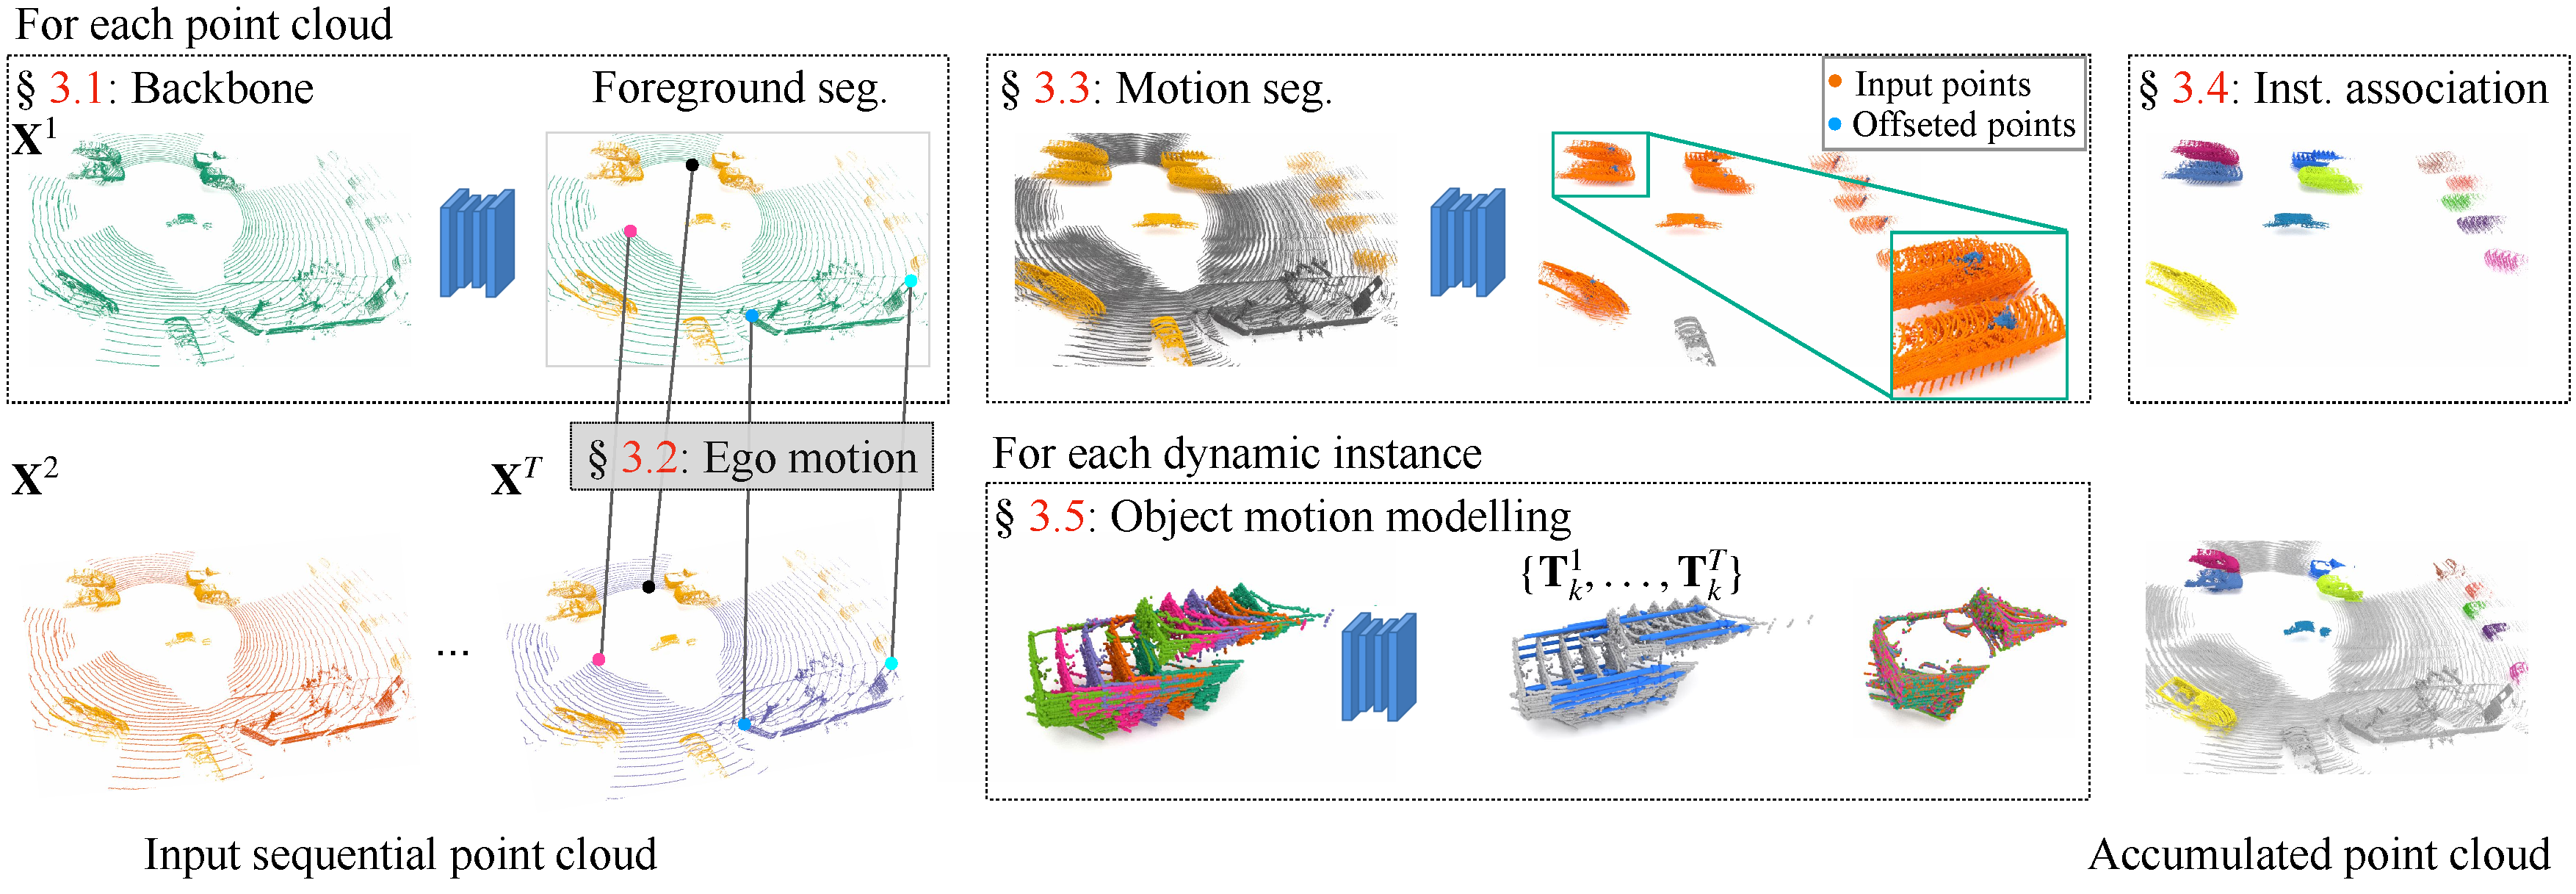
\includegraphics[width=1.0\columnwidth]{Figures/overview.pdf}
        \caption{
        Overview of \dynfl. Our method takes LiDAR scans and tracked bounding boxes of dynamic vehicles as input. \dynfl first decomposes the scene into a static background and $N$ dynamic vehicles, each modelled using a dedicated neural field. These neural fields are then composed to re-simulate LiDAR scans in dynamic scenes. Our composition technique supports various scene edits, including altering object trajectories, removing and adding reconstructed neural assets between scenes.
    }
    \label{fig:main}
\end{figure}


\paragraph{Neural fields for dynamic vehicles} 
LiDAR scans collected over time are often mis-aligned due to the motion of both the sensor and other objects in the scene. Despite applying ego-motion for aligning static background points, dynamic object points remain blurred along their trajectories. Our approach to constructing a dynamic neural scene representation is grounded in the assumption that each dynamic object only undergoes rigid motion. Therefore, we can first align them over time and reconstruct them in their \textit{canonical} coordinate frame, and then render them over time by reversing the alignment of the neural field.

Specifically, consider a dynamic vehicle $v$ 
occurring in LiDAR scans $\{\mathbf{X}^v_t\}_{t=1}^{T}$ along with the associated bounding boxes $\{\mathbf{B}^v_t \in \mathbb{R}^{3\times 8}\}_{t=1}^{T}$ in the world coordinate framework. Here each bounding box is defined by its eight corners, and the first bounding box $\mathbf{B}^v_1$ is considered as the \textit{canonical} box. We estimate the relative transformations $\{\mathbf{T}_t \in \text{SE}(3)\}_{t=2}^{T}$ between the remaining $T-1$ bounding boxes and the canonical box, expressed as $\mathbf{B}_1^v = \mathbf{T}_t \mathbf{B}_t^v$\footnote{$\mathbf{T}\mathbf{B} = \mathbf{R}\mathbf{B} + \mathbf{t}$, where $\mathbf{R}$ and $\mathbf{t}$ are the rotation and translation components of $\mathbf{T}$.}. 
Subsequently, all LiDAR measurements on the object are transformed and accumulated in its canonical coordinate frame. The vehicle $v$ is then reconstructed in its canonical space, akin to the static background, using a neural field $\mathbf{F}^v$. To render the dynamic vehicle at timestamp $t$, the corresponding rigid transformation is applied to the queried rays. The dynamic neural field can thus be expressed as: $\mathbf{F}^v_t: (\mathbf{T}_{t}\x, \mathbf{T}_{t}\dir) \mapsto (s, \intensity, \pdrop)$. The rendering process for $\mathbf{F}^v$ is the same as rendering for static neural field $\mathbf{F}_{\text{static}}$.



\section{Neural rendering of the dynamic scene}
In this section, we present the methodology for rendering LiDAR scans from the neural scene representation. We begin by revisiting the density-based volume rendering formulation for active sensors~\cite{Huang2023nfl} in \cref{sec:vol_render_background}. Subsequently, we explore the extension of this formulation to SDF-based neural scene representation in \cref{sec:sdf_vol_render}. Finally, we provide a detailed discussion on rendering LiDAR measurements from individual neural fields in~\cref{sec:dynamic_nfl_rendering} and the process of composing results from different neural fields in \cref{sec:neural_fields_composition}.



\subsection{Volume rendering for active sensor} 
\label{sec:vol_render_background}
LiDAR utilizes laser beam pulses to determine the distance to the nearest reflective surface by analyzing full waveform profile of the returned radiant power. The radiant power $P(\zeta)$ from range $\zeta$ is the result of a convolution between the pulse power $P_e(t)$ and the impulse response $H(\zeta)$, defined as~\cite{hahner2021fog,hahner2022lidar,Huang2023nfl}:
\begin{equation}
    P(\zeta) = \int_0^{2\zeta/c} P_e(t) H(\zeta - \frac{ct}{2}) \; dt\;.
\label{eq:lidar}
\end{equation}
The impulse response $H(\zeta)$ is a product of the target and sensor impulse responses: $H(\zeta) = H_T(\zeta)\cdot H_S(\zeta)$, and the individual components are expressed as:
\begin{equation}
    H_T(\zeta) = \frac{\reflectance}{\pi} \cos(\theta) \delta(\zeta - \bar{\zeta})\;, \quad  H_s(\zeta) = \transmittance^2_{\zeta} \frac{A_e}{\zeta^2}\;,
\label{eq:ht}
\end{equation}
where $\reflectance$ represents the surface reflectance, $\theta$ denotes incidence angle, $\bar{\zeta}$ is the ground truth distance to the nearest reflective surface, $\transmittance_{\zeta}$ and $A_e$ describe the transmittance at range $\zeta$ and sensor's effective area, respectively. Due to the non-differentiability introduced by the indicator function $\delta(\zeta - \bar{\zeta})$, ~\cref{eq:lidar} is non-differentiable and is thus not suitable for solving the inverse problem. NFL~\cite{Huang2023nfl} solves it by extending it into a probabilistic formulation given by:
\begin{equation}
P(\zeta) = C \cdot \frac{T^2_{\zeta} \cdot \density_\zeta  \reflectance_\zeta}{\zeta^2} \cos(\theta)\;.
\label{eq:radiance}
\end{equation}
Here, $C$ accounts for the constant values, and $\sigma_\zeta$ represents the density at range $\zeta$. The radiant can be reconstructed using the volume rendering formulation:
\begin{equation}
      P
      =\!\sum_{j=1}^N \int_{\zeta_j}^{\zeta_{j+1}}\!\!C \frac{\transmittance^2_{\zeta} \cdot \density_\zeta \reflectance_\zeta}{\zeta^2} \cos(\theta_j) \; d\zeta
      =\!\sum_{j=1}^N w_j \reflectance_{\zeta_j}',
\label{eq:radiant_inter}
\end{equation}
where the weights $w_j = 2 \opacity_{\zeta_j} \cdot\prod_{i=1}^{j-1}(1 - 2 \opacity_{\zeta_i}).$
Here $\alpha_{\zeta_j}$ is the discrete opacity at range $\zeta_j$. Please refer to~\cite{Huang2023nfl} for more details.


\subsection{SDF-based volume rendering for active sensor} 
\label{sec:sdf_vol_render}
A neural scene representation based on probabilistic density often results in surfaces with noticeable noise due to insufficient surface regularization~\cite{wang2021neus}. To address this, we opt for a signed distance-based scene representation and establish the volume rendering formulation within the framework of an active sensor. Building upon SDF-based volume rendering for passive sensors~\cite{wang2021neus}, we compute the opaque density $\tilde{\density}_{\zeta_i}$ as follows:
\begin{equation}
\tilde{\density}_{\zeta_i} = \max\left(\frac{-\frac{{\textrm{d}}\Phi_s}{{\textrm{d}} \zeta_i}(f(\zeta_i))}{\Phi_s(f(\zeta_i))},0\right),
\label{eq:sigmoid_density}
\end{equation}
where $\Phi_s(\cdot)$ represents the Sigmoid function, $f(\zeta)$ evaluates the signed distance to the surface at range $\zeta$ along the ray $\ray$. 

Next, we substitute the density $\density$ in \cref{eq:radiant_inter} with opaque density from \cref{eq:sigmoid_density} and re-evaluate the radiant power and weights as:
\begin{equation}
      P
      =\!\sum_{j=1}^N \transmittance^2_{\zeta_j} \tilde{\alpha}_{\zeta_j} \reflectance_{\zeta_j}',\quad \tilde{w}_j = 2 \tilde{\opacity}_{\zeta_j} \cdot\prod_{i=1}^{j-1}(1 - 2 \tilde{\opacity}_{\zeta_i})\;.
\end{equation}
In this context, $\tilde{\alpha}_{\zeta_j}$ is computed as:
\begin{equation}
    \tilde{\alpha}_{\zeta_j} = \max\left(\!\frac{{\Phi_s(f(\zeta_j))}^2 -{\Phi_s(f(\zeta_{j+1}))}^2}{{2\Phi_s(f(\zeta_j))}^2},0\right).
    \label{eq:new_weights}
\end{equation}
Please refer to the appendix for more details.


\subsection{Volume rendering for LiDAR measurements}
\label{sec:dynamic_nfl_rendering}
Consider rendering the LiDAR measurements from a single neural field, we employ the hierarchical sampling\cite{wang2021neus} technique to sample a total of $N_s= N_u + N_i$ points along each ray, where $N_u$ points are uniformly sampled, and $N_i$ points are probabilistically sampled based on the weights along the ray, facilitating denser sampling in proximity to the surface. Subsequently, we compute the weights for the $N_s$ points following~\cref{eq:new_weights}. The rendering of range, intensity, and ray drop for each ray can be expressed through volume rendering as follows: $y_\text{est} = \sum_{j=1}^{N_s} w_j y_j$, where $y \in \{\zeta, \intensity, \pdrop\}$.


\subsection{Neural rendering for multiple fields}\label{sec:neural_fields_composition}
Our full neural scene representation comprises $N+1$ neural fields as discussed in ~\cref{sec: decomposition}. Rendering from all these fields for each ray during inference is computationally intensive. To address this, we implement a two-stage method. In the first stage, we identify the $k+1$ neural fields, where $k \geq 0$ represents the number of dynamic fields, that are likely to intersect with a given ray. The second stage involves rendering LiDAR measurements from these selected fields individually and then integrating them into a unified set of measurements.


\paragraph{Ray intersection test}
As outlined in~\cref{sec: decomposition}, each dynamic neural field is reconstructed in its unique canonical space, defined by a corresponding canonical box. To determine neural fields intersecting with a ray at inference time, we begin by estimating the transformations $\{\mathbf{T}_t^v\}_{v=1}^N$, which convert coordinates from the world framework to each vehicle's canonical space at timestamp $t$. These transformations are determined by interpolating the training set transformations using spherical linear interpolation (SLERP)~\cite{10.1145/325334.325242}. Following this, we apply transformations to the queried ray and run intersection tests with the canonical boxes of the scenes. 


\paragraph{Neural rendering from multiple neural fields}
 After identifying the $k+1$ neural fields that potentially intersect with a ray, we perform volume rendering on each field separately, yielding $k+1$ distinct sets of LiDAR measurements. Next, we evaluate the ray drop probabilities across these fields. A ray is deemed \textit{dropped} if all neural fields indicate a drop probability $\pdrop > 0.5$. For rays not classified as dropped, we sort the estimated ranges in ascending order and select the nearest one as our final range prediction. Correspondingly, the intensity value is extracted from the same neural field associated with this closest range.

\section{Neural Scene Optimisation} \label{sec:optmisation}
Given the set of LiDAR scans and the associated tracked bounding boxes of the dynamic vehicles, we optimise our neural scene representation by minimising the loss:
\begin{equation}
    \mathcal{L} = w_{\zeta} \mathcal{L}_{\zeta} +  w_{s} \mathcal{L}_{s} + w_{\text{eik}} \mathcal{L}_{\text{eik}} + w_{\intensity} \mathcal{L}_{\intensity} + w_{\text{drop}} \mathcal{L}_{\text{drop}},
    \label{loss}
\end{equation}
where $w_{*}$ denotes respective weights, and each individual loss term $\mathcal{L}_*$ is explained below.


\paragraph{Range reconstruction loss}
For range estimation, we employ L1 loss, defined as: $\mathcal{L}_{\zeta} = \frac{1}{|\mathcal{R}|}\sum_{\ray \in \mathcal{R}}|\zeta_{est} -\zeta_{gt}|$, where $\mathcal{R}$ denotes the set of LiDAR rays, $\zeta_{est}$ and $\zeta_{gt}$ correspond to the estimated and actual ranges, respectively. 


\paragraph{Surface points' SDF regularisation} \label{sec:surfacesdf}
Acknowledging that LiDAR points mostly come from actual surface, we introduce an additional SDF regularisation term $\mathcal{L}_{s}$ that penalizes surface points' SDF values: $\mathcal{L}_{s} = \frac{1}{|\mathcal{P}|}\sum_{\mathbf{p} \in \mathcal{P}}|s(\mathbf{p})|$. Here $\mathcal{P}$ denotes the set of surface points and $s({\mathbf{p}})$ represents the SDF value of the point $\mathbf{p}$.


\paragraph{Eikonal constraint}
Following~\cite{icml2020_2086}, we utilize the Eikonal loss, $\leik$, to regularize the SDF level set. This ensures the gradient norm of the SDF is approximately one at any queried point. The loss is computed as: $\leik = \frac{1}{|\mathcal{Z}|} \sum_{\mathbf{p} \in \mathcal{Z}}( \| \nabla s(\mathbf{p}) \|_2 - 1)^2$, where $\mathcal{Z}$ is the set of all the sampled points. To stablise the training procedure, we adopt a numerical approach~\cite{li2023neuralangelo} to compute $\nabla s(\pos)$ as: 
\begin{equation}
    \nabla s(\pos) = \frac{s \left( \pos + \boldsymbol{\epsilon} \right) - s \left(\pos - \boldsymbol{\epsilon} \right)}{2 \epsilon} \;,
    \label{eqn:central_diff_normal}
\end{equation}
where the numerical step size $\epsilon$ is set to be $10^{-3}$ meters.


\paragraph{Intensity Loss}
For intensity reconstruction, we apply L2 loss, defined as: $\mathcal{L}_{\intensity} = \frac{1}{|\mathcal{R}|}\sum_{\ray \in \mathcal{R}}(\intensity_{est} -\intensity_{gt})^2.$


\paragraph{Ray drop loss}
We follow~\cite{Huang2023nfl} to supervise the ray drop estimation with a combination of a binary cross entropy loss $\mathcal{L}_{bce}$ and a Lovasz loss $\mathcal{L}_{ls}$ \cite{berman2018lovasz} as:
\begin{equation}
     \mathcal{L}_{\text{drop}} = \frac{1}{|\mathcal{R}|} \sum_{\ray \in \mathcal{R}} \left(\mathcal{L}_{bce}(p_{d, est}, {p_{d, gt}}) + \mathcal{L}_{ls}(p_{d, est}, {p_{d, gt}}) \right)\;.
     \label{eq:raydrop_loss}
\end{equation}
It's worth noting that in the context of dynamic neural fields, during training, we incorporate all LiDAR rays that intersect with the objects' bounding boxes of the scenes. A ray is classified as \textit{dropped} either if it is labeled as such in the dataset or if it does not intersect with the actual surfaces of the dynamic vehicles (\eg rays that are close but in parallel to the surfaces). This approach enhances the accuracy and realism of the reconstructed dynamic neural fields, improving the rendering fidelity at inference time. 

\section{Experiments}
\begin{figure*}[t]
  \centering
   \includegraphics[width=1\textwidth]{Figures/errormap_dynamic_3.pdf}
   
   \caption{Qualitative comparison of range estimation on \textit{Waymo Dynamic} dataset. Dynamic vehicles are zoomed in, and points are color-coded by range errors~(-100 \bwrDyNFL~100 cm).
   }
   \label{fig:errormap_dynamic}
   
\end{figure*}








\subsection{Datasets and Evaluation Protocol}\label{sec:datasets}

\paragraph{Real-world dynamic scenes} 
We construct \textit{Waymo Dynamic} dataset by selecting four representative scenes from Waymo Open dataset~\cite{sun2020scalability}, with multiple moving vehicles inside. These scenes are comprised of sequences of 50 consecutive frames. For evaluation purposes, every fifth frame is designated for testing, while the other 40 frames are allocated for training.


\paragraph{Real-world static scenes}
We also evaluate our method on four static scenes as introduced in~\cite{Huang2023nfl}. There are two settings, \textit{Waymo Interp} applies the same evaluation protocol as \textit{Waymo Dynamic}, while \textit{Waymo NVS} employs a dedicated closed-loop evaluation to validate the real novel view synthesis performance. Please refer to NFL~\cite{Huang2023nfl} for more details about this setting. 
 


\paragraph{Synthetic static scenes}  
\textit{TownClean} and \textit{TownReal} are synthetic static scenes introduced in NFL~\cite{Huang2023nfl}. They consist of 50 LiDAR scans simulated in urban street environment, using non-diverging and diverging beams, respectively. 



\paragraph{Evaluation metrics}\label{sec:metrics}
To evaluate the LiDAR range accuracy, we employ a suite of four metrics: mean absolute errors~(MAE [cm]), median absolute errors~(MedAE [cm]), Chamfer distance~(CD[cm]) and MedAE for dynamic vehicles~(MedAE Dyn[cm]). For intensity evaluation, We report root mean square error~(RMSE).
%
In addition to our primary evaluations, we assess the re-simulated LiDAR scans' realism through two auxiliary tasks: object detection and semantic segmentation. For object detection, we calculate the \textit{detection agreement}~\cite{manivasagam2020lidarsim}, both for all vehicles (Agg.~[\%]) and specifically for dynamic vehicles (Dyn.$\;$Agg.~[\%]). Regarding semantic segmentation, we measure and report recall, precision, and the intersection over union (IoU[\%]). It's important to note that the predictions on the original LiDAR scans serve as our \textit{ground truth}, against which we compare the results obtained from the re-simulated scans.




\paragraph{Baseline methods}
Regarding LiDAR simulation on static scenes, NFL~\cite{Huang2023nfl} and LiDARsim\cite{manivasagam2020lidarsim} are two closest baselines to compare to. Additionally, we include i-NGP~\cite{mueller2022instant}, DS-NeRF~\cite{kangle2021dsnerf}, and URF~\cite{rematas2022urban} for comparison. As for simulation on dynamic scenes, we compare to LiDARsim~\cite{manivasagam2020lidarsim} and UniSim~\cite{yang2023unisim}\footnote{We re-implement LiDARsim~\cite{lee2015lidar} and UniSim~\cite{yang2023unisim} as they are not open-sourced.}. Please refer to the appendix for implementation details.


\begin{table}[t]
    \setlength{\tabcolsep}{4pt}
    \renewcommand{\arraystretch}{1.2}
	\centering
	\resizebox{\columnwidth}{!}{
    \begin{tabular}{l|ccccc}
    \toprule
    Method  & MAE $\downarrow$ &  MedAE $\downarrow$ & CD $\downarrow$ & MedAE Dyn $\downarrow$ & Intensity RMSE $\downarrow$\\
    \midrule
    LiDARsim~\cite{manivasagam2020lidarsim} & 170.1 & 11.5 & 31.1 &  16.0  & 0.10\\
    Unisim~\cite{yang2023unisim} & 35.6 & 6.1 & 14.3 &14.3 & \textbf{0.05}\\
    Ours~ & \textbf{30.8} & \textbf{3.0} & \textbf{10.9} &\textbf{8.5} & \textbf{0.05}\\
    \bottomrule
    \end{tabular}
    }
    
	\caption{Evaluation of LiDAR NVS on \textit{Waymo Dynamic} dataset.}
	\label{tab:waymodynamic}
\end{table}
\begin{table}[t]
    \setlength{\tabcolsep}{4pt}
    \renewcommand{\arraystretch}{1.2}
	\centering
	\resizebox{\columnwidth}{!}{
    \begin{tabular}{l|ccc|ccc|ccc|ccc}
    \toprule
    & \multicolumn{3}{c|}{TownClean}& \multicolumn{3}{c|}{TownReal} & \multicolumn{3}{c|}{Waymo interp.} & \multicolumn{3}{c}{Waymo NVS} \\
    Method  & MAE $\downarrow$ &  MedAE $\downarrow$ & CD $\downarrow$& MAE $\downarrow$ &  MedAE $\downarrow$ & CD $\downarrow$ & MAE $\downarrow$ &  MedAE $\downarrow$ & CD $\downarrow$ & MAE $\downarrow$ &  MedAE $\downarrow$ & CD $\downarrow$\\
    \midrule
    i-NGP~\cite{mueller2022instant} &42.2 &4.1 & 17.4 & 49.8 & 4.8 & 19.9 & \textbf{26.4} & 5.5 & \textbf{11.6} & \underline{30.4} & 7.3 & 15.3\\
    DS-NeRF~\cite{kangle2021dsnerf} &41.7 & 3.9 &16.6 & 48.9 & 4.4 & 18.8 & \underline{28.2} & 6.3 & 14.5 & 30.4 & 7.2 & 16.8 \\
    URF~\cite{rematas2022urban} &43.3&4.2&16.8& 52.1 & 5.1 & 20.7 & 28.2 & 5.4 & 12.9 & 43.1 & 10.0 & 21.2 \\
    LiDARsim~\cite{manivasagam2020lidarsim} &159.6&\underline{0.8}&23.5& 162.8 & 3.8 & 27.4 & 116.3 & 15.2 & 27.6 & 160.2 & 16.2 & 34.7 \\
    NFL\cite{Huang2023nfl}  &\underline{32.0}&2.3&\underline{9.0}& \underline{39.2} & \underline{3.0} & \underline{11.5} & 30.8 & \underline{5.1} & \underline{12.1}& 32.6 & \underline{5.5} & \underline{13.2}  \\
    Ours & \textbf{26.7} & \textbf{0.7} & \textbf{6.7} &\textbf{33.9}&\textbf{2.1}&\textbf{10.4}& 28.3 & \textbf{4.7} & 12.5 & \textbf{28.6} & \textbf{4.9} & \textbf{13.0} \\
    \bottomrule
    \end{tabular}
}
    
	\caption{Evaluation of LiDAR NVS on static scenes.}
	\label{tab:waymostatic}
\end{table}
\begin{figure}[t]
  \centering
   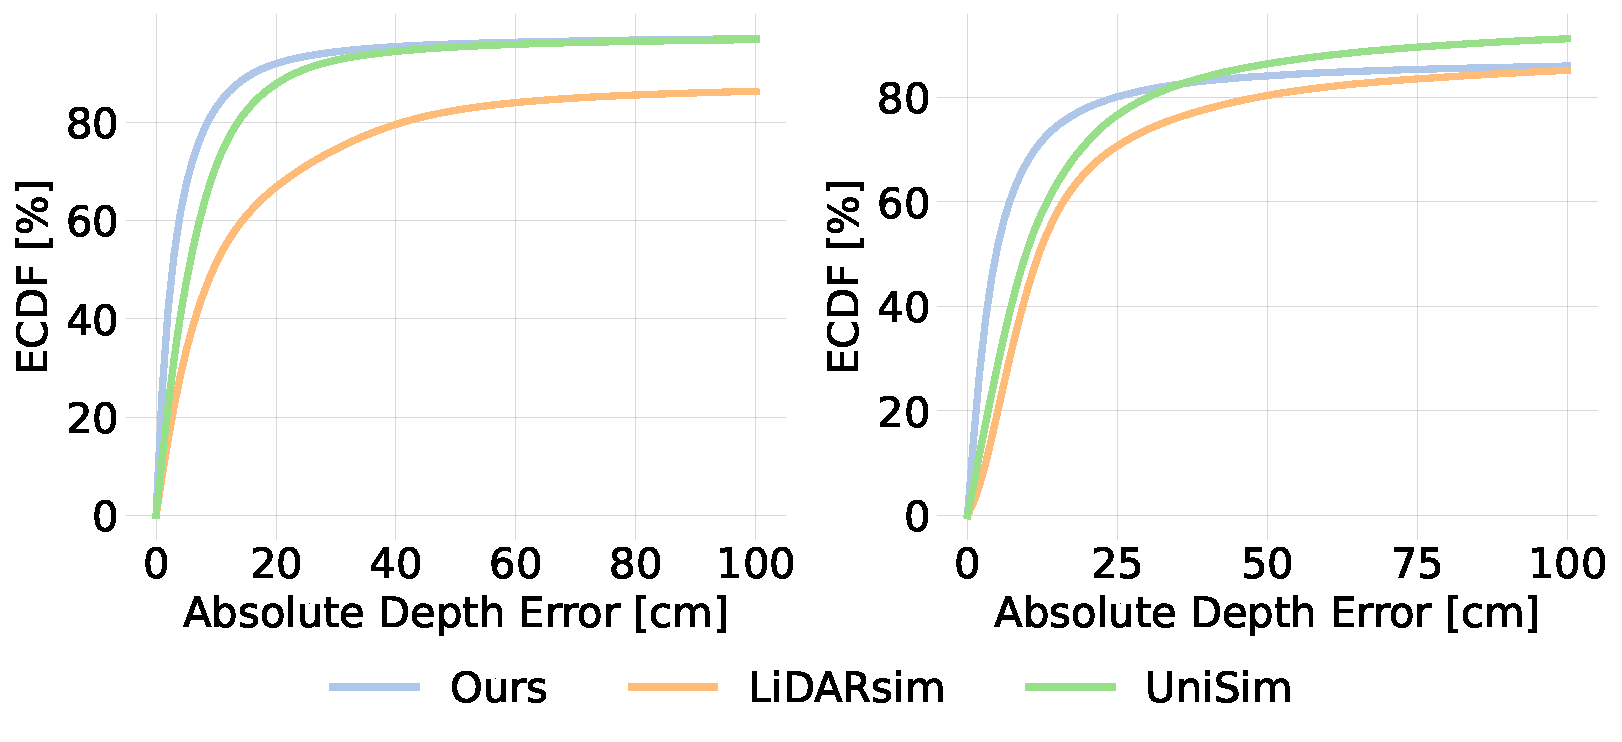
\includegraphics[width=1\columnwidth]{Figures/ecdf_3_methods.pdf}
   
        \caption{ECDF plots showcasing range errors across all the points (left) and specifically for points associated with dynamic vehicles (right). Our neural fields composition demonstrates superior performance over LiDARsim~\cite{manivasagam2020lidarsim} and UniSim~\cite{yang2023unisim}, especially in the context of dynamic vehicles.}
   \label{fig:ecdf}
   
\end{figure}
\begin{figure}[t]
    \centering
        \includegraphics[width=1\columnwidth]{Figures/errormap_static.pdf}
        
        \caption{Qualitative results of range estimation. Regions with gross errors (-100 \bwrDyNFL~100 cm) are highlighted.
        }
    \label{fig:error_map}
\end{figure}
\subsection{LiDAR Novel View Synthesis Evaluation} \label{sec:lidar_eval}
\paragraph{LiDAR NVS in dynamic scenes}
Quantitative comparisons with baseline methods are detailed in~\cref{tab:waymodynamic}. \dynfl notably outperforms LiDARsim~\cite{manivasagam2020lidarsim} and UniSim~\cite{yang2023unisim} in range reconstruction. This improvement is largely due to our SDF-based neural scene representation, which incorporates the physical aspects of LiDAR sensing. Additionally, our method employs a ray drop test when rendering multiple neural fields, leading to a more accurate reconstruction of dynamic vehicles, as evidenced in~\cref{fig:errormap_dynamic} and further supported by the data in~\cref{fig:ecdf}.


\begin{figure*}[t]
    \centering
        \includegraphics[width=1.0\textwidth]
        {Figures/sensor_manipulation.pdf}
        
        \caption{LiDAR novel view synthesis by changing sensor elevation angle~($\theta$), poses~($x,y,z$) and number of beams on \textit{Waymo Dynamic} dataset. The points are color-coded by the intensity values (0 \bwrDyNFL~0.25).}
    \label{fig:lidar_nvs}
\end{figure*}
\paragraph{LiDAR NVS in static scenes}
In addition to dynamic scenes, we evaluate \dynfl against baseline methods in static scenarios, with the results detailed in~\cref{tab:waymostatic} and~\cref{fig:error_map}. \dynfl excels in reconstructing geometry in most cases. A key observation is its superior performance in reconstructing planar regions (\eg the ground shown in~\cref{fig:error_map}), especially when compared to NFL~\cite{Huang2023nfl}, which also uses a neural field for surface representation. This improvement is largely due to the enhanced surface regularizations provided by our advanced SDF-based surface modeling approach.


\begin{table}[t]
    \setlength{\tabcolsep}{4pt}
    \renewcommand{\arraystretch}{1.2}
	\centering
	\resizebox{0.5\columnwidth}{!}{
    \small
    \begin{tabular}{l|ccc}
    \toprule
    Datasets  & MAE $\downarrow$ &  MedAE $\downarrow$ & CD $\downarrow$ \\
    \midrule
    TownClean~ & 26.7(\textcolor{green}{-1.5}) & 0.7(\textcolor{green}{-0.2}) & 6.7(\textcolor{green}{-0.5})\\
    Waymo Interp~ & 28.3 (\textcolor{red}{0.1}) & 4.7 (\textcolor{green}{-0.2}) & 12.5 (\textcolor{green}{-0.1})\\
    Waymo Dynamic~ & 30.8 (\textcolor{green}{-0.3}) & 3.0 (\textcolor{green}{-0.2}) & 10.9 (\textcolor{green}{-0.3})\\
    \bottomrule
    \end{tabular}
    }
    
	\caption{Ablation study of volume rendering for active sensing.}
	\label{tab:active_sensing}
\end{table}
\begin{table}[t]
    \setlength{\tabcolsep}{4pt}
    \renewcommand{\arraystretch}{1.2}
	\centering
	\resizebox{0.5\columnwidth}{!}{
    \small
    \begin{tabular}{l|ccc}
    \toprule
    Datasets  & MAE $\downarrow$ &  MedAE $\downarrow$ & CD $\downarrow$ \\
    \midrule
    TownReal~ & 33.9(\textcolor{green}{-3.3}) & 2.1(\textcolor{green}{-0.0}) & 10.4(\textcolor{green}{-1.2})\\
    Waymo Interp~ & 28.3 (\textcolor{green}{-0.3}) & 4.7 (\textcolor{green}{-0.1}) & 12.5 (\textcolor{green}{-0.3})\\
    \bottomrule
    \end{tabular}
    }
    
	\caption{Ablation study of the surface points' SDF regularisation.}
	\label{tab:surface_sdf}
\end{table}
\begin{figure}[t]
  \centering
   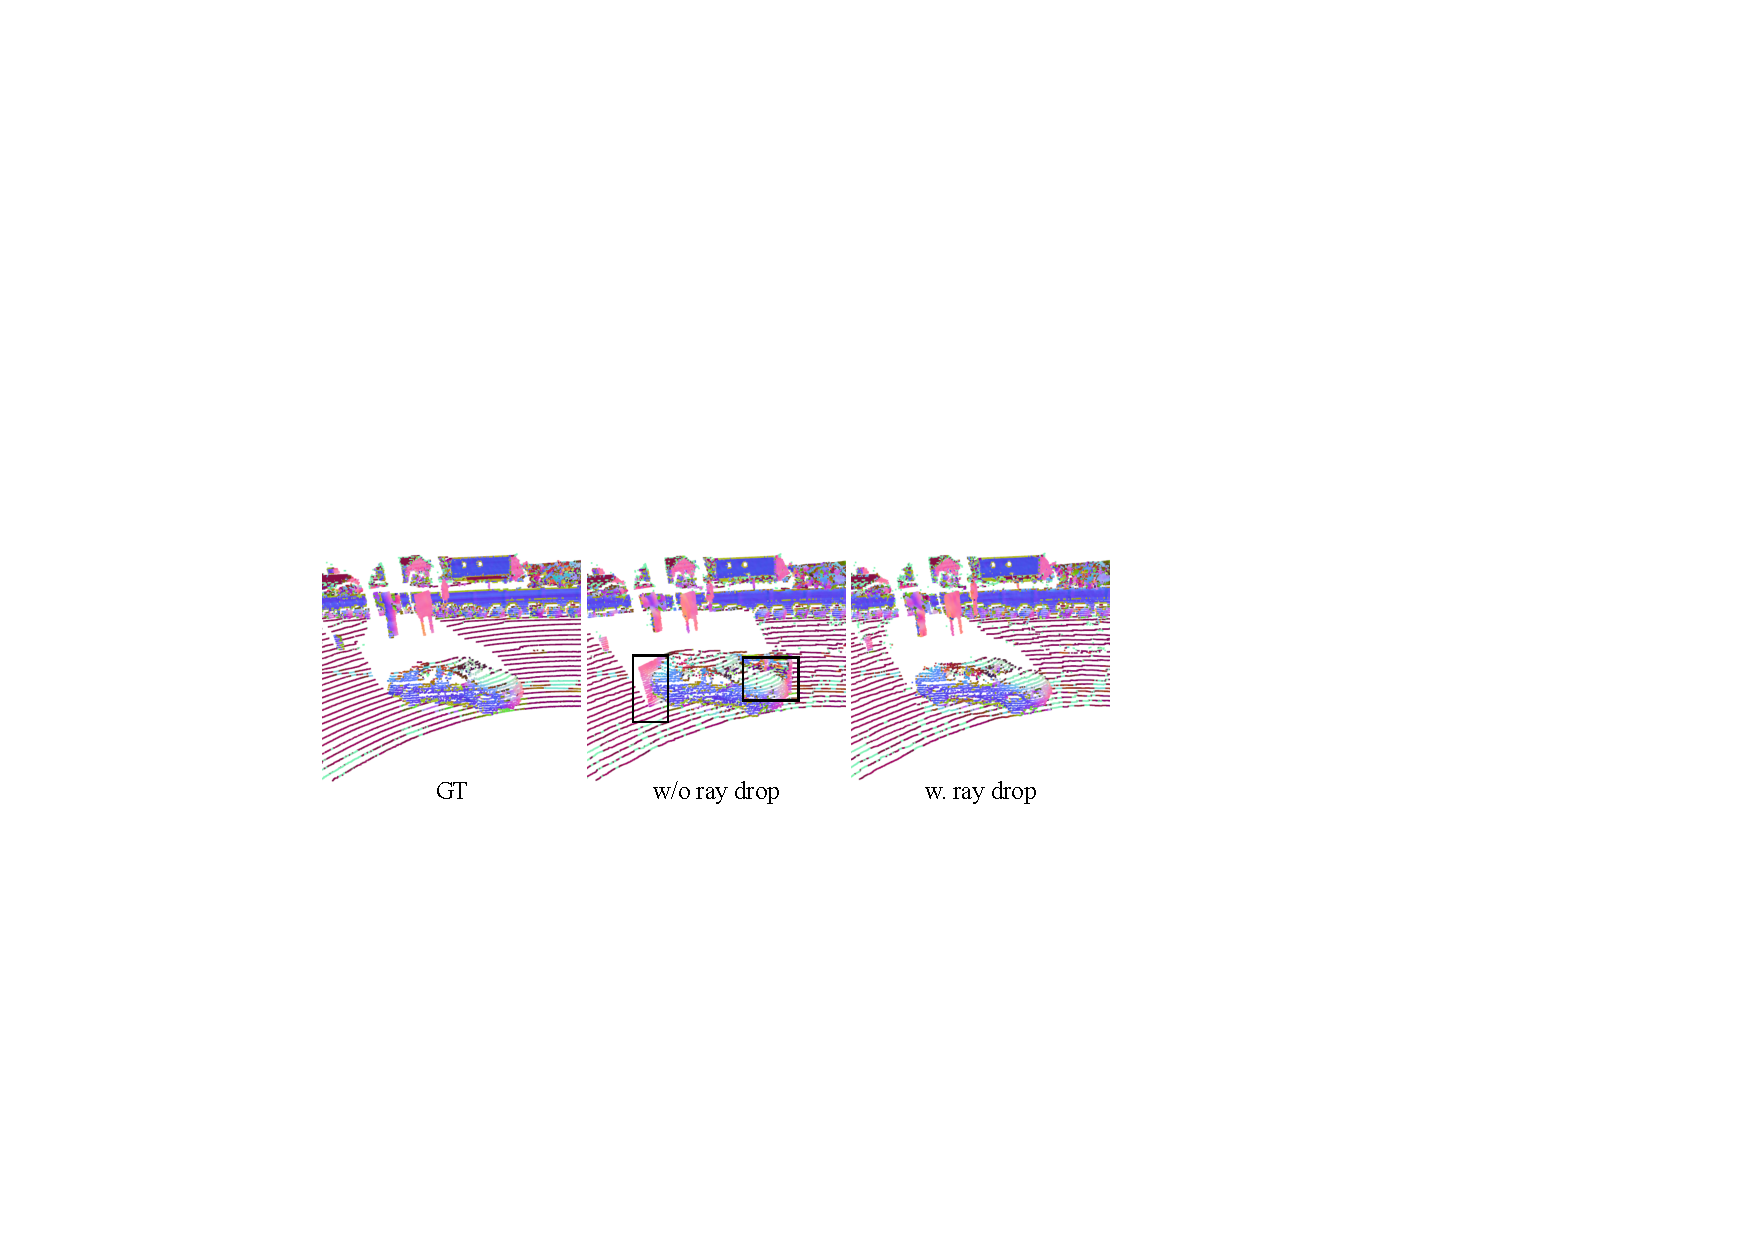
\includegraphics[width=1\linewidth]{Figures/intersectiontest.pdf}
   
   \caption{
   Qualitative results on \textit{Waymo Dynamic} dataset. Our model equipped with a ray drop module effectively composites multiple neural fields, re-simulating LiDAR scans of high quality.
   }
   % \caption{These figures exemplify the effectiveness of our field composition method leveraging ray drop probability from dynamic neural field. When all intersected rays are rendered for the dynamic neural field, noticeable artifacts appear due to disturbances from irrelevant fields (middle figure). The figures on the right showcase the complete composition method.
   % }
   % \caption{
   % }
    
   \label{fig:ablation_raydrop}
\end{figure}

\begin{figure}[t]
    \centering
        \includegraphics[width=0.8\columnwidth]{Figures/detection_result.pdf}
        \caption{Object detection results on \textit{Waymo Dynamic} dataset. The ground truth and predicted bounding boxes are marked in \textcolor{red}{red} and \textcolor{blue}{blue}, respectively.}
    \label{fig:detection}
    
\end{figure}
% \begin{table}[t]
% 	\centering
% 	\resizebox{0.8\columnwidth}{!}{
% 		\begin{tabular}{@{}lcccccccc@{}}
% 			\toprule
%              & \multicolumn{1}{c}{GT} & \multicolumn{3}{c}{Ours} & \multicolumn{3}{c}{LiDARSim\cite{manivasagam2020lidarsim}} \\
% 			  \cmidrule(r){2-2}\cmidrule(r){3-5} \cmidrule(l){6-8}
% 			Threshold & AP$\uparrow$ & \multicolumn{1}{c}{AP$\uparrow$}& \multicolumn{1}{c}{Agg.$\uparrow$}& \multicolumn{1}{c}{Dyn. Agg.$\uparrow$} & \multicolumn{1}{c}{AP$\uparrow$} & \multicolumn{1}{c}{Agg.$\uparrow$}& \multicolumn{1}{c}{Dyn. Agg.$\uparrow$} \\
% 			\midrule
% 			IoU$>$0.7 &0.85  &0.86 & \textbf{0.77}& \textbf{0.71}& \textbf{0.90} & 0.76 & 0.68\\
% 			IoU$>$0.5 &\textbf{0.98}  & 0.96 & \textbf{0.87}& \textbf{0.76}& 0.95 & 0.86& \textbf{0.76} \\
% 			\bottomrule
% 		\end{tabular}
% 	}
% 	\caption{Object detection results on \textit{Waymo Dyanmic} datasets.}
    
% 	\label{tab:detection}
% \end{table}

\begin{table}[t]
	\centering
		\begin{tabularx}{\columnwidth}{l|YYYYYYY}
			\toprule
             & \multicolumn{1}{c}{GT} & \multicolumn{3}{c}{Ours} & \multicolumn{3}{c}{LiDARSim\cite{manivasagam2020lidarsim}} \\
			  \cmidrule(r){2-2}\cmidrule(r){3-5} \cmidrule(l){6-8}
			Threshold & AP$\uparrow$ & \multicolumn{1}{c}{AP$\uparrow$}& \multicolumn{1}{c}{Agg.$\uparrow$}& \multicolumn{1}{c}{Dyn. Agg.$\uparrow$} & \multicolumn{1}{c}{AP$\uparrow$} & \multicolumn{1}{c}{Agg.$\uparrow$}& \multicolumn{1}{c}{Dyn. Agg.$\uparrow$} \\
			\midrule
			IoU$>$0.7 &0.85  &0.86 & \textbf{0.77}& \textbf{0.71}& \textbf{0.90} & 0.76 & 0.68\\
			IoU$>$0.5 &\textbf{0.98}  & 0.96 & \textbf{0.87}& \textbf{0.76}& 0.95 & 0.86& \textbf{0.76} \\
			\bottomrule
		\end{tabularx}
	\caption{Object detection results on \textit{Waymo Dyanmic} datasets.}
    
	\label{tab:detection}
\end{table}
% \begin{table}[t]
% \setlength{\tabcolsep}{4pt}
% \renewcommand{\arraystretch}{1.2}
% \centering
% \resizebox{0.8\columnwidth}{!}{
% \begin{tabular}{l|ccc|ccc}
% \toprule
% & \multicolumn{3}{c|}{Vehicle} & \multicolumn{3}{c}{Background} \\
% Method & Recall $\uparrow$ & Precision $\uparrow$ & IoU $\uparrow$ & Recall $\uparrow$ & Precision $\uparrow$ & IoU $\uparrow$ \\
% \midrule
% i-NGP~\cite{muller2022instant} & \underline{93.2} & 85.9 & 80.9 & 98.3 & \underline{99.2} & 97.6\\
% DS-NeRF~\cite{deng2021depth} & 90.7 & \underline{87.1} & 80.2 & \underline{98.5} & 98.9 & 97.4\\
% URF~\cite{rematas2021urban} & 87.8 & 81.7 & 73.7 & 98.0 & 98.4 & 96.5\\
% Lidarsim~\cite{manivasagam2020lidarsim} & 90.5 & 70.5 & 65.9 & 94.9 & 99.0 & 94.0\\
% NFL density~\cite{Huang2023nfl}& \textbf{95.9} & 87.0 & \textbf{83.9} & 98.3 & \textbf{99.5} & \textbf{97.8}\\
% Ours & 90.5 & \textbf{89.2} & \underline{82.3} & \textbf{98.8} & 98.9 & \underline{97.7}\\
% \bottomrule
% \end{tabular}
% }
% 
% \caption{Semantic segmentation results on \textit{Waymo NVS} dataset.}
% \label{tab:sem_seg_nvs}
% \end{table}



\begin{table}[t]
\setlength{\tabcolsep}{4pt}
\renewcommand{\arraystretch}{1.2}
\centering
\resizebox{0.99\columnwidth}{!}{
\begin{tabular}{l|ccc|ccc}
\toprule
& \multicolumn{3}{c|}{Vehicle} & \multicolumn{3}{c}{Background} \\
Method & Recall $\uparrow$ & Precision $\uparrow$ & IoU $\uparrow$ & Recall $\uparrow$ & Precision $\uparrow$ & IoU $\uparrow$ \\
\midrule
i-NGP~\cite{mueller2022instant} & 91.8 & 83.6 & 78.1 & 97.9 & 99.2 & 97.1\\
DS-NeRF~\cite{kangle2021dsnerf} & 89.3 & 84.8 & 77.3 & 98.1 & 98.8 & 97.0\\
URF~\cite{rematas2021urban} & 86.9 & 79.8 & 72.0 & 97.7 & 98.5 & 96.2\\
Lidarsim~\cite{manivasagam2020lidarsim} & 89.6 & 68.9 & 64.0 & 94.5 & 98.9 & 93.5\\
NFL~\cite{Huang2023nfl}& \textbf{94.5} & 84.8 & 80.9 & 97.8 & \textbf{99.4} & \textbf{97.3}\\
Ours & 90.5 & \textbf{88.4} & \textbf{81.1} & \textbf{98.5} & 98.7 & \textbf{97.3}\\
\bottomrule
\end{tabular}
}

\caption{Semantic segmentation results on \textit{Waymo NVS} dataset.}
\label{tab:sem_seg_nvs_ours}

\end{table}




\subsection{Ablation Study}
\paragraph{SDF-based volume rendering for active sensing}
We begin by assessing the efficacy of our SDF-based volume rendering for active sensor, the results are shown in~\cref{tab:active_sensing}. When compared to our baseline that uses the SDF-based volume rendering for passive sensing, \dynfl demonstrates enhanced performance in both synthetic (\textit{TownClean}) and real-world (\textit{Waymo Interp} and \textit{Waymo Dynamic}) datasets, indicating the importance of incorporating the physical sensing process of LiDAR in addressing the inverse problem.


\paragraph{Neural fields composition} 
To validate the efficacy of our two-stage neural field composition approach, we compare it with an alternative approach utilized in UniSim~\cite{yang2023unisim}. The results are shown in~\cref{tab:waymodynamic}. UniSim~\cite{yang2023unisim} blends different neural fields by sampling points from all intersected neural fields, followed by a single evaluation of volume rendering to produce the final LiDAR scan. In contrast, our method independently renders from each intersecting neural field first, and then combines these measurements into a final measurement using a ray drop test (\cf~\cref{fig:ablation_raydrop}). This approach leads to a notable improvement in geometry reconstruction over UniSim~\cite{yang2023unisim}, exemplified by our method halving the Median Absolute Error (MedAE) across all points. This enhancement is even more evident when focusing solely on points related to dynamic vehicles (\cf~\cref{fig:ecdf}).
% 

\paragraph{Surface points' SDF constraint}
We examine the importance of the surface points' SDF constraint discussed in ~\cref{sec:optmisation} on \textit{Town Real} and \textit{Waymo Interp} datasets. The results shown in \cref{tab:surface_sdf} suggest that our method yields improved geometry reconstruction quality by additionally enforcing LiDAR points to have zero SDF values. 


\subsection{Auxiliary Task Evaluations} 
\label{sec:downstream}
To assess the fidelity of our neural re-simulation and gauge the domain gap between re-simulated and real scans, we evaluate their applicability in two downstream tasks: object detection and semantic segmentation.


\paragraph{Object detection}
We utilize the pre-trained FSDv2~\cite{fan2023fsdv2} model for object detection and conduct evaluations on the re-simulated LiDAR scans within the \textit{Waymo Dynamic} dataset. Our results are compared against those from LiDARsim~\cite{manivasagam2020lidarsim}, with the findings detailed in~\cref{tab:detection} and~\cref{fig:detection}. Notably, \dynfl exhibits a more substantial detection agreement with the predictions on real LiDAR scans. This indicates a higher fidelity in our re-simulations and a reduced domain gap relative to actual scans.


\paragraph{Semantic segmentation}
For semantic segmentation, we use the pre-trained SPVNAS model~\cite{tang2020searching}, with the results presented in~\cref{tab:sem_seg_nvs_ours}. \dynfl improves over baseline methods according to most evaluation metrics, underscoring the realism of our re-simulated LiDAR scans.



\subsection{Scene Editing}
Beyond LiDAR novel view synthesis by adjusting the sensor configurations (\cf \cref{fig:lidar_nvs}), we additionally demonstrate the practicality of our compositional neural fields approach through two scene editing applications.

\begin{figure}[t]
    \includegraphics[width=1.0\linewidth]{Figures/vehicle_insertion.pdf}
    
    \caption{
    Qualitative results of object removal and insertion. \dynfl seamlessly inserts the neural asset (truck) into a new scene attributed to our superior compositional rendering scheme. In contrast, UniSim~\cite{yang2023unisim} struggles to accurately model geometry.
    }
    \label{fig:vehicle_insertion}
\end{figure}
\paragraph{Insert object from one scene into another}
Our explicit neural scene de-composition and flexible composition technique enable seamless insertion and removal of neural assets across scenes. As demonstrated in~\cref{fig:vehicle_insertion}, we are able to replace a car from one scene with a truck from another scene, achieving accurate reconstruction of both geometry and intensity. In contrast, UniSim~\cite{yang2023unisim} struggles to preserve high quality geometry. This highlights the significant potential of our approach in generating diverse and realistic LiDAR scans for autonomous driving scenarios.

\begin{figure}[t]
    \includegraphics[width=1.0\columnwidth]{Figures/trajectory_manipulation.pdf}
    
    \caption{Qualitative results of object trajectory manipulation. The truck can be successfully detected after manipulation, indicating high-realism LiDAR re-simulation achieved by \dynfl.}
    \label{fig:traj}
    
\end{figure}
\paragraph{Manipulate the trajectory of dynamic objects}
\dynfl also facilitates the manipulation of moving objects' trajectories by simply adjusting their relative poses to the canonical bounding box. Representative results are shown in ~\cref{fig:traj}. The high realism of our re-simulation is also indicated by the successful detection of inserted virtual objects.

\section{Limitations and Future Work}
We present DyNFL, a compositional neural fields approach for LiDAR re-simulation. Our method excels previous art in both static and dynamic scenes, offering powerful scene editing capabilities that open up opportunities for generating diverse and high-quality scenes, to evaluate an autonomy system trained only on real data in closed-loop.

Despite achieving the state-of-the-art performance, there are still limitations we aim to address in future work. Firstly, \dynfl faces challenges in view synthesis of dynamic vehicles from unseen angles. This difficulty arises from the complexity of creating an a-priori model that can accurately complete unseen regions and simulate point cloud noise, ray drops patterns etc. Secondly, our method currently relies on object detection and tracking annotations, and its performance may be compromised when given inaccurate labels. Overcoming this dependency, exploring 4D representations while retaining scene editing flexibility, stands out as a crucial challenge for future research.


\paragraph{Acknowledgements.}
{Or Litany is a Taub fellow and is supported by the Azrieli Foundation Early Career Faculty Fellowship.}

\clearpage
\section{Appendix}
In this supplementary material, we first provide additional information about the datasets for our evaluations and implementation details of our proposed method in~\cref{sec:sup_dataset}. Next, we present more qualitative results in~\cref{sec:sup_visual}. Please also check the supplemental video for more results showcasing our performance. Finally, we provide the complete derivations of the SDF-based volume rendering for active sensor in~\cref{sec:sup_sdf_vol_render}. 

\section{Datasets and implementation details}\label{sec:sup_dataset}
\subsection{Datasets}
\paragraph{\textit{Waymo Dynamic}} For the \textit{Waymo Dynamic} dataset, we take them from 4 scenes of \textit{Waymo Open Dataset}~\cite{sun2020scalability}. There are multiple moving vehicles inside each scene. 50 consecutive frames are taken from each scene for our evaluation. The vehicles are deemed as \textit{dynamic} if the speed is $>1\,$m/s. in any of the 50 frames. The corresponding scene IDs on \textit{Waymo Open Dataset} for our selected scenes are shown as follows:
\begin{table}[!h]
    \setlength{\tabcolsep}{4pt}
    \renewcommand{\arraystretch}{1.2}
	\centering
	\resizebox{0.8\columnwidth}{!}{
    \begin{tabular}{l|c}
    \toprule
    & Scene ID \\
    \midrule
    Scene 1 & 1083056852838271990\_4080\_000\_4100\_000 \\
    Scene 2 & 13271285919570645382\_5320\_000\_5340\_000 \\
    Scene 3 & 10072140764565668044\_4060\_000\_4080\_000 \\
    Scene 4 & 10500357041547037089\_1474\_800\_1494\_800 \\
    \bottomrule
    \end{tabular}
    }
\end{table}

\subsection{Implementation details}
\paragraph{Ours} 
Our model is implemented based on nerfstudio\cite{nerfstudio}. For the static neural field, we sample $N_s=512$ points in total, with $N_u=256$ uniformly sampled points and $N_i=256$ weighted sampled points with 8 upsample steps. In each upsample step, 32 points are sampled based on the weight distribution of the previously sampled points. For each dynamic neural field, we sample $N_s=128$ points in total, with $N_u=64$ uniformly sampled points and $N_i=64$ weighted sampled points with 4 upsample steps. During training, we minimize the loss function using the Adam~\cite{kingma2014adam} optimiser, with an initial learning rate of 0.005. It linearly decays to 0.0005 towards the end of training. For the loss weights, we use $w_{\zeta}=3, w_{e}=50, w_{\text{drop}}=0.15, w_{s}=1$, and  $w_{\text{eik}}=0.3$. The batch size is 4096 and we train the model for 60000 iterations on a single RTX3090 GPU with float32 precision.

\paragraph{LiDARsim} We re-implement the LiDARsim~\cite{manivasagam2020lidarsim} as one of our baselines. 
First, we estimated point-wise normal vectors by considering all points within a 20 cm radius ball within the training set. Following this, we applied voxel down-sampling~\cite{tang2022torchsparse}, employing a 4 cm voxel size to reconstruct individual disk surfels at each point. The surfel orientation is defined based on the estimated normal vector. During inference, we apply the ray-surfel intersections test to determine the intersection points, thus the range and intensity values. We select a fixed surfel radius of 6 cm for the \textit{Waymo} dataset and 12 cm for the \textit{Town} dataset.
To handle dynamic vehicles, we follow LiDARsim~\cite{manivasagam2020lidarsim} by aggregating the LiDAR points for each vehicle from all the training frames and representing them in the \textit{canonical} frame of each vehicle. During inference, we transform all the aggregated vehicle points from their \textit{canonical} frames to the world frame and run ray-surfel intersection.

\paragraph{UniSim} 
We re-implement UniSim's~\cite{yang2023unisim} rendering process for LiDAR measurements by replacing our ray-drop test-based neural fields composition method with its joint rendering method. For every ray $\mathbf{r} (\mathbf{o},\mathbf{d})$, we begin by conducting an intersection test with all dynamic bounding boxes in the scene to identify the near and far limits. We then uniformly sample 512 points along each ray, assigning each point to either a dynamic neural field, if it falls within a dynamic bounding box, or to the static neural field otherwise. After sampling, we query the SDF and intensity values from the relevant neural fields. Finally, using the SDF-based volume rendering formula in Eq.~\ref{eq:depth_render} for active sensors, we calculate the weights and perform the rendering. Note that we use the same neural field architecture as in our method.
\begin{figure*}[t!]
  \centering
   \includegraphics[width=1\textwidth]{Figures_sup/4_scenes_sup.pdf}
   \caption{Visualization of 4 selected scenes from \textit{Waymo Dynamic} dataset. For each scene, we aggregate 50 frames. In the first row, points are color-coded by the intensity values(0 ~\bwrDyNFL~ 0.25). In the second row, dynamic vehicles are painted as \textcolor{yellow}{yellow}.}
   \label{fig:4_scenes_supp}
\end{figure*}

\begin{figure*}[t!]
  \centering
   \includegraphics[width=1\textwidth]{Figures_sup/supp_scene_edit.pdf}
   \caption{Visualization of scene editing capabilities. We showcase 3 kinds of scene editing capabilities including vehicle removal(left), trajectory manipulation(middle) and vehicle insertion(right). The first row represents the original scenes, the second row demonstrates the scenes after editing. All points are color-coded by the intensity values(0 ~\bwrDyNFL~ 0.25).}
   \label{fig:scene_editing_supp}
\end{figure*}

\section{More qualitative results}\label{sec:sup_visual}
In this section, we provide more qualitative results. In \cref{fig:4_scenes_supp}, we showcase the 4 scenes from \textit{Waymo dynamic} dataset. We show additional scene editing results in~\cref{fig:scene_editing_supp}. Please check the supplementary videos for more qualitative results.

\clearpage
\clearpage
\section{SDF-based volume rendering for active sensor}\label{sec:sup_sdf_vol_render}
In this section, we start by introducing the preliminary of NeRF~\cite{mildenhall2020nerf} following terminology as described in~\cite{tagliasacchi2022volume}. Then we provide the full derivation of the SDF-based volume rendering for active sensor. 

\subsection{Preliminary}\label{sec:supp_pre}
\paragraph{Density}
For a ray emitted from the origin $\origin \in \real^3$ towards direction $\dir \in \real^3$, the \textit{density} $\density_\zeta$ at range $\zeta$ indicates the likelihood of light interacting with particles at that point $\ray_\zeta = \origin + \zeta \dir$. This interaction can include absorption or scattering of light. In passive sensing, density $\density$ is a critical factor in determining how much light from the scene's illumination is likely to reach the sensor after passing through the medium.
\paragraph{Transmittance} quantifies the likelihood of light traveling through a given portion of the medium without being scattered or absorbed. Density is closely tied to the transmittance function $\transmittance(\zeta)$, which indicates the probability of a ray traveling over the interval $[0, \zeta)$ without hitting any particles. Then the probability $\transmittance(\zeta {+} d\zeta)$ of \emph{not} hitting a particle when taking a differential step $d\zeta$ is equal to $\transmittance(\zeta)$, the likelihood of the ray reaching $\zeta$, times $(1 - d\zeta \cdot \density(\zeta))$, the probability of not hitting anything during the step:
% 
\begin{align}
\transmittance(\zeta+d\zeta) =& \transmittance(\zeta) \cdot (1 - d\zeta \cdot \density(\zeta))
\\
\frac{\transmittance(\zeta+d\zeta) - \transmittance(\zeta)}{d\zeta} \equiv& \transmittance'(\zeta) = -\transmittance(\zeta) \cdot \sigma(\zeta) 
\label{eq:derivative}
\end{align}
% 
We solve the differential equation as follows:
%
\begin{align}
\transmittance'(\zeta) &= -\transmittance(\zeta) \cdot \density(\zeta) \\
\frac{\transmittance'(\zeta)}{\transmittance(\zeta)} &= -\density(\zeta) \\
\int_a^b \frac{\transmittance'(\zeta)}{\transmittance(\zeta)} \; d\zeta &= -\int_a^b \density(\zeta) \; d\zeta \\
\left. \log \transmittance(\zeta) \right|_a^b &= -\int_a^b \density(\zeta) \; d\zeta \\
\transmittance(a \rightarrow b) \equiv \frac{\transmittance(b)}{\transmittance(a)} &= \exponential{-\int_a^b \density(\zeta) \; d\zeta}   
\end{align}
% 
Hence, for a ray segment between $\zeta_0$ and $\zeta$, transmittance is given by:

\begin{equation}
\transmittance_{\zeta_0 \rightarrow \zeta} \equiv \frac{\transmittance_{\zeta}}{\transmittance_{\zeta_0}} = exp({-\int_{\zeta_0}^\zeta \density_t dt})\;,
\label{eq:trans_ab}
\end{equation}
which leads to following factorization of the transmittance:
\begin{equation}
\transmittance_{\zeta} = \transmittance_{0 \rightarrow \zeta_0} \cdot \transmittance_{\zeta_0 \rightarrow \zeta}\;.
\label{eq:factor}
\end{equation}

\paragraph{Opacity}Opacity is the complement of transmittance and represents the fraction of light that is either absorbed or scattered in the medium. In a homogeneous medium with constant density $\density$  the opacity for a segment $[\zeta_j, \zeta_{j+1}]$ of length $\Delta \zeta$ is given by $\opacity_{\zeta_j} = 1 - exp(-\density \cdot \Delta \zeta)$
\subsection{SDF-based volume rendering for active sensor}\label{sec:sdf_active}
NeuS\cite{wang2021neus} derives the opaque density based on the SDF which is:
\begin{equation}
\begin{split}
\density_{\zeta_i} =&  \max\left(\frac{-\frac{d\Phi_s}{d\zeta_i}(f(\zeta_i))}{\Phi_s(f(\zeta_i))},0\right)\\
                  =& \max\left(\frac{-(\nabla f(\zeta_i)\cdot \mathbf{v})\phi_s(f(\zeta_i))}{\Phi_s(f(\zeta_i))}, 0\right)
\end{split}
\label{eq:sigmoid_density}
\end{equation}
where $\Phi_s$ represents the Sigmoid function, $f$ is the SDF function that maps a range $\zeta$ to the SDF value of the point position $\origin + \dir * \zeta$. Note that the integral term is computed by
\begin{equation}
\int \frac{-(\nabla f(\zeta)\cdot \mathbf{v})\phi_s(f(\zeta))}{\Phi_s(f(\zeta))}d\zeta = -\ln(\Phi_s(f(\zeta))) + C,
\label{eq:intergration_density}
\end{equation}
% We can then calculate the accumulated transmittance from \ref{eq:trans_ab} using \ref{eq:intergration_density}:
% % 
% \begin{align}
% \transmittance_\zeta = \transmittance(0 \rightarrow \zeta) 
% % &= \prod_{k=1}^{n-1} \transmittance(t_k \rightarrow t_{k+1}) 
% &= \exponential{- \int_{0}^{\zeta} \density(t) \; dt} 
% = \Phi_s(f(\zeta))
% \label{eq:trans_const}
% \end{align}
We extend the density-based volume rendering for active sensor to SDF-based. Starting from the passive SDF-based volume rendering \cite{wang2021neus}, We substitute the density $\tilde{\density}$ with opaque density in \ref{eq:sigmoid_density}
and evaluate the radiant power integrated from ray segment [a,b] with constant reflectivity $\reflectivity_a$.

Consider the case where $-(\nabla f(\zeta)\cdot \mathbf{v})>0$ within the ray segment $[a,b]$, we have
\begin{align}
P(a \rightarrow b)
&= \int_a^b \transmittance^2(a\rightarrow t) \cdot \tilde{\density}_t \cdot \reflectivity(t)  \; dt
\\
&= \reflectivity_a \int_a^b \transmittance^2(a\rightarrow t) \cdot \tilde{\density}_t \; dt
\\
&= \reflectivity_a \int_a^b \exponential{-\int_a^t 2\tilde{\density}(u) \; du} \cdot \tilde{\density}_t \; dt
\\
&= \reflectivity_a \int_a^b \exponential{-2\int_a^t \tilde{\density}(u) \; du} \cdot \tilde{\density}_t \; dt
\\
&= \reflectivity_a \int_a^b \exponential{\left. 2\ln(\Phi_s(f(u)))\right|_a^t} \cdot \tilde{\density}_t \; dt
\\
% &= \reflectivity_a \int_a^b \exponential{2\ln(\Phi_s(f(t))) - 2\ln(\Phi_s(f(a)))} \cdot \tilde{\density}_t \; dt \\
&= \reflectivity_a \int_a^b \exponential{2\ln(\Omega_t) - 2\ln(\Omega_a)} \cdot \tilde{\density}_t \; dt 
\\
&= \reflectivity_a \int_a^b \frac{{\Omega_t}^2}{{\Omega_a}^2} \cdot \tilde{\density}_t \; dt ~~~~\text{\textbf{let} $\Omega_x = \Phi_s(f(x))$}
\\
&= \frac{\reflectivity_a}{{\Omega_a}^2} \int_a^b {\Omega_t}^2 \cdot \tilde{\density}_t \; dt 
\\
&= \frac{\reflectivity_a}{{\Omega_a}^2} \int_a^b -\frac{d\Phi_s}{dt}(f(t)) \cdot \Phi_s(f(t)) \; dt 
% \quad \text{$\tilde{\density}_t = \frac{-\frac{d\Phi_s}{d t}(f(t))}{\Phi_s(f(t))}$}
\\
&= \frac{\reflectivity_a}{{\Omega_a}^2} ( \left. -\frac{1}{2}{\Phi_s(f(t))}^2 \right|_a^b) \\
&= \frac{\reflectivity_a}{{\Omega_a}^2} (\frac{1}{2}{\Phi_s(f(a))}^2 -\frac{1}{2}{\Phi_s(f(b))}^2 )\\
&= \frac{{\Phi_s(f(a))}^2 -{\Phi_s(f(b))}^2}{{2\Phi_s(f(a))}^2} \cdot \reflectivity_a 
% \quad \text{$T_a$ = $\Phi_s(f(a))$}
\label{eq:homogeneous}
\end{align}
%\cref{eq:trans_const}

Consider the case where $-(\nabla f(\zeta)\cdot \mathbf{v})<0$ within the ray segment $[a,b]$, we have
\begin{align}
P(a \rightarrow b)
&= \int_a^b \transmittance^2(a\rightarrow t) \cdot \tilde{\density}_t \cdot \reflectivity(t)  \; dt
\\
&= \int_a^b \transmittance^2(a\rightarrow t) \cdot 0 \cdot \reflectivity(t)  \; dt
\\
&= 0
\end{align}
Hence we conclude 
\begin{align}
P(a \rightarrow b)
&= \max\left(\frac{{\Phi_s(f(a))}^2 -{\Phi_s(f(b))}^2}{{2\Phi_s(f(a))}^2},0\right) \cdot \reflectivity_a 
\end{align}

\paragraph{Volume rendering of piecewise constant data}
Combining the above, we can evaluate the volume rendering integral through a medium with piecewise constant reflectivity:
% 
\begin{align}
P(\zeta_{N+1}) &= \sum_{n=1}^N \int_{\zeta_n}^{\zeta_{n+1}} \transmittance^2(\zeta) \cdot \tilde{\density}_{\zeta} \cdot \reflectivity_{\zeta_n} \; d\zeta
\\
&= \sum_{n=1}^N \int_{\zeta_n}^{\zeta_{n+1}} \transmittance^2_{\zeta_n} \cdot \transmittance^2(\zeta_n \shortto \zeta) \cdot \tilde{\density}_{\zeta} \cdot \reflectivity_{\zeta_n} \; d\zeta 
% &&\text{from \ref{eq:factor}}
\\
&= \sum_{n=1}^N \transmittance^2_{\zeta_n}  \int_{\zeta_n}^{\zeta_{n+1}} \transmittance^2(\zeta_n \rightarrow \zeta) \cdot \tilde{\density}_{\zeta} \cdot \reflectivity_{\zeta_n} \; d\zeta \\
% &&\text{constant}
% \\
&=\sum_{n=1}^N \transmittance^2_{\zeta_n} P(\zeta_n \rightarrow \zeta_{n+1})
\\
&= \sum_{n=1}^N \transmittance^2_{\zeta_n} \cdot \tilde{\weight}_{\zeta_n} \cdot \reflectivity_{\zeta_n},
% &&\text{from \ref{eq:homogeneous}}
\end{align}

where 
\begin{align}
\tilde{\weight}_{\zeta_n} \equiv \max\left(\frac{{\Phi_s(f(\zeta_n)}^2 -{\Phi_s(f(\zeta_{n+1}))}^2}{{2\Phi_s(f(\zeta_n))}^2},0\right)
\end{align}
% 
% This leads to the volume rendering equations from NeRF~\cite[Eq.3]{mildenhall2020nerf}:
% % 
% \begin{align}
% P(\zeta_{N+1}) = \sum_{n=1}^N \transmittance^2_{\zeta_n} \cdot \frac{{\Phi_s(f(\zeta_n))}^2 -{\Phi_s(f(\zeta_{n+1}))}^2}{{2\Phi_s(f(\zeta_n))}^2} \cdot \reflectivity_{\zeta_n}
% \label{eq:final_radiant}
% \end{align}
% % 
% Since the opacity is always greater than 0, we can express the opacity as
% \begin{equation}
%     \tilde{\weight}_{\zeta_n} \equiv max(\frac{{\Phi_s(f(\zeta_n))}^2 -{\Phi_s(f(\zeta_{n+1}))}^2}{{2\Phi_s(f(\zeta_n))}^2}, 0)
%     \label{eq:opacity}
% \end{equation}

The discrete accumulated transmittance $\transmittance$ can be calculated as follows:

Consider the case where $-(\nabla f(\zeta)\cdot \mathbf{v}) > 0$ in $[\zeta_n, \zeta_{n+1}]$: 
%
\begin{align}
\transmittance_{\zeta_n} 
&=\prod_{i=1}^{n-1}(\exp(-\int_{\zeta_n}^{\zeta_{n+1}}\tilde{\density}_\zeta \; d\zeta) \\
&= \prod_{i=1}^{n-1}(\frac{\Phi_s(f(\zeta_{n+1}))}{\Phi_s(f(\zeta_n))})\\
\transmittance^2_{\zeta_n}
&= \prod_{i=1}^{n-1}(\frac{{\Phi_s(f(\zeta_{n+1}))}^2}{{\Phi_s(f(\zeta_n))}^2})\\
&= \prod_{i=1}^{n-1}(1-2\tilde{\weight}_{\zeta_n})
\label{eq:dicrete_transmittance}
\end{align}

Consider the case where $-(\nabla f(\zeta)\cdot \mathbf{v}) < 0$ in $[\zeta_n, \zeta_{n+1}]$: 
\begin{align}
\transmittance_{\zeta_n} 
&=\prod_{i=1}^{n-1}(\exp(-\int_{\zeta_n}^{\zeta_{n+1}}\tilde{\density}_\zeta \; d\zeta) = \prod_{i=1}^{n-1}(1)
\\
\transmittance^2_{\zeta_n} &= \prod_{i=1}^{n-1}(1^2) = \prod_{i=1}^{n-1}(1-2\tilde{\weight}_{\zeta_n})
\end{align}
In conclusion, the radiant power can be reformulated as:

\begin{align}
P(\zeta_{N+1}) = \sum_{n=1}^N \transmittance^2_{\zeta_n} \cdot \tilde{\weight}_{\zeta_n} \cdot \reflectivity_{\zeta_n}
\label{eq:final_radiant2}
\end{align}
where $\transmittance^2_{\zeta_n} = \prod_{i=1}^{n-1}(1-2\tilde{\weight}_{\zeta_i})$


\paragraph{Depth volume rendering of piecewise constant data}

Note that $\tilde{\weight}_{\zeta_n} \in [0, 0.5], \transmittance^2_{\zeta_n} \in [0,1], \sum_{n=1}^N \transmittance^2_{\zeta_n} \cdot \tilde{\weight}_{\zeta_n} = 0.5$, for depth volumetric rendering, we have 
\begin{align}
    \zeta = \sum_{n=1}^N 2 \cdot \transmittance^2_{\zeta_n} \cdot \tilde{\weight}_{\zeta_n} \cdot \zeta_n
    =\sum_{n=1}^N w_n \cdot \zeta_n
    \label{eq:depth_render}
\end{align}
where $w_n = 2\tilde{\weight}_{\zeta_n} \cdot \prod_{i=1}^{n-1}(1-2\tilde{\weight}_{\zeta_i})$


% Conclusions + Outlook
% \chapter{Conclusions}
\label{chap:conclusion}
placeholder

\section{Lessons Learned}
placeholder
% -------
\section{Limitations}
placeholder

\section{Outlook}
placeholder


%** Switch to appendix-mode in Latex.
%
\appendix

%** I would like to have the appendices enumerated by Alphabetical
%   characters.
\renewcommand{\thepart}{\Alph{part}}


\renewcommand\bibsection{\chapter{Bibliography}}
\bibliographystyle{plain}
\bibliography{references}                % name your BibTeX data base

%!TEX root = thesis.tex

\chapter{Curriculum Vitae}
%\label{chap:cv}
%\addcontentsline{toc}{chapter}{\nameref{chap:cv}}
\textbf{Personal data}\\

\begin{tabular}{ p{4cm} l }
  {Name} & {\textbf{Shengyu Huang}}\\
  {} & {}\\
  {Date of birth} & {\textbf{17.11.1995}}\\
  {} & {}\\
  {Nationality} & {\textbf{China}}\\
  {} & {}\\
\end{tabular}\\

\vspace{0.5cm}

\noindent
\textbf{Education}\\

\begin{tabular}{ p{4cm} l }
  {Oct. 2020 - Nov. 2024} & {\textbf{ETH Zurich, Switzerland}}\\
  {} & {PhD Student} \\
  {} & {}\\
  {Sep. 2018 - Aug. 2020} & {\textbf{ETH Zurich, Switzerland}}\\
  {} & {M.Sc. in Geomatik} \\
  {} & {}\\
  {Sep. 2014 - Aug. 2018} & {\textbf{Tongji University, China}}\\
  {} & {BSc. in Surveying and Mapping Engineering} \\
\end{tabular}\\

\vspace{0.5cm}

\noindent
\textbf{Professional Experience}\\

\begin{tabular}{ p{4cm} l }
  {Oc. 2020 - Nov. 2024} & {\textbf{ETH Zurich, Switzerland}}\\
  {} & {Research and Teaching Assistant} \\
  {} & {}\\
  {Jul 2023 - Dec 2023} & {\textbf{Google, Munich, Germany}}\\
  {} & {Student Researcher} \\
  {} & {}\\
  {Apr 2022 - Dec 2022} & {\textbf{NVIDIA, Zurich, Switzerland}}\\
  {} & {Research Scientist Intern} \\
\end{tabular}

\chapter{List of Publications}

\begin{enumerate}
    \item \textbf{\textbf{S. Huang}}, M. Usvyatsov, K. Schindler. ”Indoor Scene Recognition in 3D.” IROS, 2020.
    \item \textbf{S. Huang}*, Z. Gojcic*, M. Usvyatsov, A. Wieser, K. Schindler. ”PREDATOR: Registration of 3D Point Clouds with Low Overlap.” CVPR, 2021. (Oral)
    \item \textbf{S. Huang}, Z. Gojcic, J. Huang, A. Wieser, K. Schindler ”Dynamic 3D Scene Analysis by Point Cloud Accumulation.” ECCV, 2022.
    \item \textbf{S. Huang}, Z. Gojcic, Z. Wang, F. William, Y. Kasten, S. Fidler, K. Schindler, O. Litany ”Neural LiDAR Fields for Novel View Synthesis.” ICCV, 2023.
    \item H. Wu, X. Zuo, S. Leutenegger, Or Litany, K. Schindle, \textbf{S. Huang} ”Dynamic LiDAR Re-simulation using Compositional Neural Fields.” CVPR, 2024. (Hightlight)
    \item L. Zhu, \textbf{S. Huang}, K. Schindler, I. Armeni. ”Living Scenes: Multi-object Relocalization and Reconstruction in Changing 3D Environments.” CVPR, 2024. (Hightlight)
    \item B. Ke, A. Obukhov, \textbf{S. Huang}, N. Metzger, R. Daudt, K. Schindler. ”Repurposing Diffusion-Based Image Generators for Monocular Depth Estimation.” CVPR, 2024. (Oral, Best Paper Award Candidate)
    \item Y. Jia, L. Hoyer, \textbf{S. Huang}, T. Wang, L. Gool, K. Schindler, A. Obukhov. ”DGInStyle: DomainGeneralizable Semantic Segmentation with Image Diffusion Models and Stylized Semantic Control.” ECCV, 2024.
    \item Z. Wang, T. Shen, J. Gao, \textbf{S. Huang}, J. Munkberg, J. Hasselgren, Z. Gojcic, W. Chen, S. Fidler ”Neural Fields meet Explicit Geometric Representations for Inverse Rendering of Urban Scenes.” CVPR, 2023.
    \item L. Zhu, Y. Jia, \textbf{S. Huang}, N. Meyer, A. Wieser, K. Schindler, J. Aaron ”DeFlow: Self-supervised 3D Motion Estimation of Debris Flow.” CVPR Workshop, 2023. (Best Paper Award)
    \item C. Stucker, B. Ke, Y. Yue, \textbf{S. Huang}, I. Armeni, K. Schindler ”ImpliCity: City Modeling from Satellite Images with Deep Implicit Occupancy Fields.” ISPRS Congress, 2022. (Best Young Author Award)
    \item T. Sun, Y. Hao, \textbf{S. Huang}, S. Savarese, K. Schindler, M. Pollefeys, I. Armeni ”Nothing stands still: A spatiotemporal benchmark on 3d point cloud registration under large geometric and temporal change.” arxiv, 2023
\end{enumerate}
\end{document}